% uWaterloo Thesis Template for LaTeX
% Last Updated June 14, 2017 by Stephen Carr, IST Client Services
% FOR ASSISTANCE, please send mail to rt-IST-CSmathsci@ist.uwaterloo.ca

% Effective October 2006, the University of Waterloo
% requires electronic thesis submission. See the uWaterloo thesis regulations at
% https://uwaterloo.ca/graduate-studies/thesis.

% DON'T FORGET TO ADD YOUR OWN NAME AND TITLE in the "hyperref" package
% configuration below. THIS INFORMATION GETS EMBEDDED IN THE PDF FINAL PDF DOCUMENT.
% You can view the information if you view Properties of the PDF document.

% Many faculties/departments also require one or more printed
% copies. This template attempts to satisfy both types of output.
% It is based on the standard "book" document class which provides all necessary
% sectioning structures and allows multi-part theses.

% DISCLAIMER
% To the best of our knowledge, this template satisfies the current uWaterloo requirements.
% However, it is your responsibility to assure that you have met all
% requirements of the University and your particular department.
% Many thanks for the feedback from many graduates that assisted the development of this template.

% -----------------------------------------------------------------------

% By default, output is produced that is geared toward generating a PDF
% version optimized for viewing on an electronic display, including
% hyperlinks within the PDF.

% E.g. to process a thesis called "mythesis.tex" based on this template, run:

% pdflatex mythesis	-- first pass of the pdflatex processor
% bibtex mythesis	-- generates bibliography from .bib data file(s)
% makeindex         -- should be run only if an index is used
% pdflatex mythesis	-- fixes numbering in cross-references, bibliographic references, glossaries, index, etc.
% pdflatex mythesis	-- fixes numbering in cross-references, bibliographic references, glossaries, index, etc.

% If you use the recommended LaTeX editor, Texmaker, you would open the mythesis.tex
% file, then click the PDFLaTeX button. Then run BibTeX (under the Tools menu).
% Then click the PDFLaTeX button two more times. If you have an index as well,
% you'll need to run MakeIndex from the Tools menu as well, before running pdflatex
% the last two times.

% N.B. The "pdftex" program allows graphics in the following formats to be
% included with the "\includegraphics" command: PNG, PDF, JPEG, TIFF
% Tip 1: Generate your figures and photos in the size you want them to appear
% in your thesis, rather than scaling them with \includegraphics options.
% Tip 2: Any drawings you do should be in scalable vector graphic formats:
% SVG, PNG, WMF, EPS and then converted to PNG or PDF, so they are scalable in
% the final PDF as well.
% Tip 3: Photographs should be cropped and compressed so as not to be too large.

% To create a PDF output that is optimized for double-sided printing:
%
% 1) comment-out the \documentclass statement in the preamble below, and
% un-comment the second \documentclass line.
%
% 2) change the value assigned below to the boolean variable
% "PrintVersion" from "false" to "true".

% --------------------- Start of Document Preamble -----------------------

% Specify the document class, default style attributes, and page dimensions
% For hyperlinked PDF, suitable for viewing on a computer, use this:
\documentclass[letterpaper,12pt,titlepage,oneside,final]{book}

% For PDF, suitable for double-sided printing, change the PrintVersion variable below
% to "true" and use this \documentclass line instead of the one above:
%\documentclass[letterpaper,12pt,titlepage,openright,twoside,final]{book}

% Some LaTeX commands I define for my own nomenclature.
% If you have to, it's better to change nomenclature once here than in a
% million places throughout your thesis!
\newcommand{\package}[1]{\textbf{#1}} % package names in bold text
\newcommand{\cmmd}[1]{\textbackslash\texttt{#1}} % command name in tt font
\newcommand{\href}[1]{#1} % does nothing, but defines the command so the
    % print-optimized version will ignore \href tags (redefined by hyperref pkg).
%\newcommand{\texorpdfstring}[2]{#1} % does nothing, but defines the command
% Anything defined here may be redefined by packages added below...

% This package allows if-then-else control structures.
\usepackage{ifthen}
\newboolean{PrintVersion}
\setboolean{PrintVersion}{false}
% CHANGE THIS VALUE TO "true" as necessary, to improve printed results for hard copies
% by overriding some options of the hyperref package below.

%\usepackage{nomencl} % For a nomenclature (optional; available from ctan.org)
\usepackage{amsmath,amssymb,amstext} % Lots of math symbols and environments
\usepackage[pdftex]{graphicx} % For including graphics N.B. pdftex graphics driver

% Hyperlinks make it very easy to navigate an electronic document.
% In addition, this is where you should specify the thesis title
% and author as they appear in the properties of the PDF document.
% Use the "hyperref" package
% N.B. HYPERREF MUST BE THE LAST PACKAGE LOADED; ADD ADDITIONAL PKGS ABOVE
\usepackage[pagebackref=false]{hyperref} % with basic options
		% N.B. pagebackref=true provides links back from the References to the body text. This can cause trouble for printing.
\hypersetup{
    plainpages=false,       % needed if Roman numbers in frontpages
    unicode=false,          % non-Latin characters in Acrobat’s bookmarks
    pdftoolbar=true,        % show Acrobat’s toolbar?
    pdfmenubar=true,        % show Acrobat’s menu?
    pdffitwindow=false,     % window fit to page when opened
    pdfstartview={FitH},    % fits the width of the page to the window
    pdftitle={uWaterloo\ LaTeX\ Thesis\ Template},    % title: CHANGE THIS TEXT!
%    pdfauthor={Author},    % author: CHANGE THIS TEXT! and uncomment this line
%    pdfsubject={Subject},  % subject: CHANGE THIS TEXT! and uncomment this line
%    pdfkeywords={keyword1} {key2} {key3}, % list of keywords, and uncomment this line if desired
    pdfnewwindow=true,      % links in new window
    colorlinks=true,        % false: boxed links; true: colored links
    linkcolor=blue,         % color of internal links
    citecolor=green,        % color of links to bibliography
    filecolor=magenta,      % color of file links
    urlcolor=cyan           % color of external links
}
\ifthenelse{\boolean{PrintVersion}}{   % for improved print quality, change some hyperref options
\hypersetup{	% override some previously defined hyperref options
%    colorlinks,%
    citecolor=black,%
    filecolor=black,%
    linkcolor=black,%
    urlcolor=black}
}{} % end of ifthenelse (no else)

% package adeed
\usepackage{subfigure}
\usepackage{amsmath}
\usepackage{amssymb}
\usepackage{mathptmx}
\usepackage{graphicx}
\usepackage{amsfonts}
\usepackage{bbm}
\usepackage{fullpage}
\usepackage{multirow}
\usepackage{booktabs}
\usepackage{tabularx}
\usepackage[figuresright]{rotating}
\usepackage[mathscr]{euscript}
\usepackage{amstext}
\usepackage{tabularx}
\usepackage[numbers]{natbib}
\usepackage{lineno,xcolor}
\usepackage{listings}
\usepackage{setspace}
\usepackage{amsmath}
\usepackage{amssymb}
\usepackage{epsfig}
\usepackage{fancybox}
\usepackage{listings}
\usepackage{url}
\usepackage{epstopdf}
\usepackage[lined,ruled]{algorithm2e}
\usepackage{amsmath}
\usepackage{amssymb}
\usepackage{amsthm}
\usepackage{threeparttable}
\numberwithin{equation}{section}
\newtheorem{thm}{Theorem}[section]
\newtheorem{lem}{Lemma}
\newtheorem{prop}{Proposition}
\newtheorem{cor}{Corollary}
\theoremstyle{definition}
\newtheorem{definition}{Definition}[section]
%\newtheorem{pf}{Proof}

\newcommand*{\Scale}[2][4]{\scalebox{#1}{$#2$}}%
\newcommand*{\Resize}[2]{\resizebox{#1}{!}{$#2$}}%
\newcommand{\model}{\textsc{GRU}_\delta}
\newcommand{\modelT}{\textsc{GRU}_{\textsc{total}}}
\newcommand{\modelL}{\textsc{GRU}_{\textsc{local}}}
\newcommand{\modelN}{\textsc{NN}_\delta}
\newcommand{\vt}[1]{\mathbf{#1}}
\newcommand{\vw}{\mathbf{w}}
\newcommand{\vb}{\mathbf{b}}
%\newcommand{\pm}{\stackrel{+}{-}}
\newcommand{\vx}{\mathbf{x}}
\newcommand{\vi}{\mathbf{in}}
\newcommand{\vo}{\mathbf{o}}
\newcommand{\vxt}{\tilde{\mathbf{x}}}
\newcommand{\vy}{\mathbf{y}}
\newcommand{\impsigma}{\breve{\sigma}}
\newcommand{\barK}{\overline{K}}
\newcommand{\barC}{\overline{C}}
\newcommand{\vz}{\mathbf{z}}
\newcommand{\fnp}{\tilde{f}}
\newcommand{\vu}{\mathbf{u}}
\newcommand{\vs}{\mathbf{s}}
\newcommand{\vc}{\mathbf{c}}
\newcommand{\E}{\mathbf{E}}
\newcommand{\HK}{\mathcal{H}_K}
\newcommand{\XS}{\mathcal{X}}
\newcommand{\DS}{\Delta S}
\newcommand{\Heston}{\textsc{Heston}}
\newcommand{\DVmkt}{\Delta V^{mkt}}
\newcommand{\DT}{\Delta t}
\newcommand{\vuu}{\mathbf{\widetilde u}}
\newcommand{\Real}{\mathbb{R}}
\newcommand{\vdot}[2]{{#1}^T{#2}}
\DeclareMathOperator*{\argmin}{\arg\!\min}
\newcommand{\sym}{\textsc{sym}}
\newcommand{\BS}{\textsc{BS}}
\newcommand{\LOF}{\textsc{lof}}
\newcommand{\svm}{\textsc{svm}}
\newcommand{\AMflag}{\text{mFLAG}}
\newcommand{\rw}{\textsc{rw}}
\newcommand{\diag}{\textsc{diag}}
\newcommand{\sign}{\textsc{sign}}
\newcommand{\MeanAbs}{\E(|\DVmkt-\DS \delta |)}
\newcommand{\Cluster}{\textsc{C}}
\newcommand{\bi}{\text{bi}}
\newcommand{\g}{\mathbf{g}}
\newcommand{\vv}{\mathbf{v}}
\newcommand{\valpha}{\pmb{\widehat{\alpha}}}
\newcommand{\vK}{\mathbb{K}}
\newcommand{\vV}{\pmb{\breve{V}}}
\newcommand{\e}{\mathbf{e}}
\newcommand{\vol}{\Upsilon}
\newcommand{\vd}{\mathbf{d}}
\newcommand{\vh}{\mathbf{h}}
\newcommand{\vf}{\mathbf{f}}
\newcommand{\vW}{\pmb{W}}
\newcommand{\vU}{\pmb{U}}
\newcommand{\np}{\text{np}}
\newcommand{\pt}{^{+\Delta t}}
\newcommand{\norm}{\text{norm}}
\newcommand{\row}{\text{row}}
\newcommand{\Vmkt}{V^{mkt}}
\newcommand{\Smkt}{S}
\newcommand{\vecVmkt}{\mathbb{V}}
\newcommand{\Ncut}{\text{Ncut}}
\newcommand{\half}{\frac{1}{2}}
\newcommand{\DKLs}{\bf\textsc{DKL}_{\text{SPL}}}
\newcommand{\DRNNc}{\bf\textsc{DRNN}_{\text{C}}}
\newcommand{\DKLg}{\bf\textsc{DKL}_{\text{RBF}}}
\newcommand{\IKLs}{\bf\textsc{IKL}_{\text{SPL}}}
\newcommand{\IKLg}{\bf\textsc{IKL}_{\text{RBF}}}
\newcommand{\LVF}{\textsc{LVF}}
\newcommand{\Del}{\delta_{\textsc{BS}}}
\newcommand{\SABR}{\bf\textsc{SABR}_{\text{MV}}}
\newcommand{\MV}{\bf \textsc{MV}}

\usepackage{tikz}
\usetikzlibrary{shapes}
\usetikzlibrary{arrows}
\usetikzlibrary{positioning, fit, arrows.meta}
\usetikzlibrary{decorations.pathmorphing}
\usepackage{xparse}
\usetikzlibrary{calc}
\usepackage{tkz-graph}
\usetikzlibrary{backgrounds,automata}
\usepackage{atbegshi}% http://ctan.org/pkg/atbegshi
%\AtBeginDocument{\AtBeginShipoutNext{\AtBeginShipoutDiscard}}



\usepackage[automake,toc,abbreviations]{glossaries-extra} % Exception to the rule of hyperref being the last add-on package
% If glossaries-extra is not in your LaTeX distribution, get it from CTAN (http://ctan.org/pkg/glossaries-extra),
% although it's supposed to be in both the TeX Live and MikTeX distributions. There are also documentation and
% installation instructions there.

% Setting up the page margins...
% uWaterloo thesis requirements specify a minimum of 1 inch (72pt) margin at the
% top, bottom, and outside page edges and a 1.125 in. (81pt) gutter
% margin (on binding side). While this is not an issue for electronic
% viewing, a PDF may be printed, and so we have the same page layout for
% both printed and electronic versions, we leave the gutter margin in.
% Set margins to minimum permitted by uWaterloo thesis regulations:
\setlength{\marginparwidth}{0pt} % width of margin notes
% N.B. If margin notes are used, you must adjust \textwidth, \marginparwidth
% and \marginparsep so that the space left between the margin notes and page
% edge is less than 15 mm (0.6 in.)
\setlength{\marginparsep}{0pt} % width of space between body text and margin notes
\setlength{\evensidemargin}{0.125in} % Adds 1/8 in. to binding side of all
% even-numbered pages when the "twoside" printing option is selected
\setlength{\oddsidemargin}{0.125in} % Adds 1/8 in. to the left of all pages
% when "oneside" printing is selected, and to the left of all odd-numbered
% pages when "twoside" printing is selected
\setlength{\textwidth}{6.375in} % assuming US letter paper (8.5 in. x 11 in.) and
% side margins as above
\raggedbottom

% The following statement specifies the amount of space between
% paragraphs. Other reasonable specifications are \bigskipamount and \smallskipamount.
\setlength{\parskip}{\medskipamount}

% The following statement controls the line spacing.  The default
% spacing corresponds to good typographic conventions and only slight
% changes (e.g., perhaps "1.2"), if any, should be made.
\renewcommand{\baselinestretch}{1} % this is the default line space setting

% By default, each chapter will start on a recto (right-hand side)
% page.  We also force each section of the front pages to start on
% a recto page by inserting \cleardoublepage commands.
% In many cases, this will require that the verso page be
% blank and, while it should be counted, a page number should not be
% printed.  The following statements ensure a page number is not
% printed on an otherwise blank verso page.
\let\origdoublepage\cleardoublepage
\newcommand{\clearemptydoublepage}{%
  \clearpage{\pagestyle{empty}\origdoublepage}}
\let\cleardoublepage\clearemptydoublepage

% Define Glossary terms (This is properly done here, in the preamble. Could be \input{} from a file...)
% Main glossary entries -- definitions of relevant terminology
\newglossaryentry{computer}
{
name=computer,
description={A programmable machine that receives input data,
               stores and manipulates the data, and provides
               formatted output}
}

% Nomenclature glossary entries -- New definitions, or unusual terminology
\newglossary*{nomenclature}{Nomenclature}
\newglossaryentry{dingledorf}
{
type=nomenclature,
name=dingledorf,
description={A person of supposed average intelligence who makes incredibly brainless misjudgments}
}

% List of Abbreviations (abbreviations type is built in to the glossaries-extra package)
\newabbreviation{aaaaz}{AAAAZ}{American Association of Amature Astronomers and Zoologists}

% List of Symbols
\newglossary*{symbols}{List of Symbols}
\newglossaryentry{rvec}
{
name={$\mathbf{v}$},
sort={label},
type=symbols,
description={Random vector: a location in n-dimensional Cartesian space, where each dimensional component is determined by a random process}
}

\makeglossaries

%======================================================================
%   L O G I C A L    D O C U M E N T -- the content of your thesis
%======================================================================
\begin{document}

% For a large document, it is a good idea to divide your thesis
% into several files, each one containing one chapter.
% To illustrate this idea, the "front pages" (i.e., title page,
% declaration, borrowers' page, abstract, acknowledgements,
% dedication, table of contents, list of tables, list of figures,
% nomenclature) are contained within the file "uw-ethesis-frontpgs.tex" which is
% included into the document by the following statement.
%----------------------------------------------------------------------
% FRONT MATERIAL
%----------------------------------------------------------------------
% T I T L E   P A G E
% -------------------
% Last updated June 14, 2017, by Stephen Carr, IST-Client Services
% The title page is counted as page `i' but we need to suppress the
% page number. Also, we don't want any headers or footers.
\pagestyle{empty}
\pagenumbering{roman}

% The contents of the title page are specified in the "titlepage"
% environment.
\begin{titlepage}
        \begin{center}
        \vspace*{1.0cm}

        \Huge
        {\bf Data-Driven Models: An Alternative Discrete Hedging Strategy }

        \vspace*{1.0cm}

        \normalsize
        by \\

        \vspace*{1.0cm}

        \Large
        Ke Nian \\

        \vspace*{3.0cm}

        \normalsize
        A thesis \\
        presented to the University of Waterloo \\
        in fulfillment of the \\
        thesis requirement for the degree of \\
        Doctor of Philosophy \\
        in \\
        Computer Science \\

        \vspace*{2.0cm}

        Waterloo, Ontario, Canada, 2023 \\

        \vspace*{1.0cm}

        \copyright\ Ke Nian 2023 \\
        \end{center}
\end{titlepage}

% The rest of the front pages should contain no headers and be numbered using Roman numerals starting with `ii'
\pagestyle{plain}
\setcounter{page}{2}

\cleardoublepage % Ends the current page and causes all figures and tables that have so far appeared in the input to be printed.
% In a two-sided printing style, it also makes the next page a right-hand (odd-numbered) page, producing a blank page if necessary.


% E X A M I N I N G   C O M M I T T E E (Required for Ph.D. theses only)
% Remove or comment out the lines below to remove this page
\begin{center}\textbf{Examining Committee Membership}\end{center}
  \noindent
The following served on the Examining Committee for this thesis. The decision of the Examining Committee is by majority vote.
  \bigskip

  \noindent
\begin{tabbing}
Internal-External Member: \=  \kill % using longest text to define tab length
External Examiner: \>  undetermined \\
\> Professor, School of Computer Science, University of Undetermined \\
\end{tabbing}
  \bigskip

  \noindent
\begin{tabbing}
Internal-External Member: \=  \kill % using longest text to define tab length
Supervisor(s): \> Yuying Li \\
\> Professor, School of Computer Science, University of Waterloo \\
\end{tabbing}
  \bigskip

  \noindent
  \begin{tabbing}
Internal-External Member: \=  \kill % using longest text to define tab length
Internal Examiner: \>  Justin W.L. Wan \\
\> Professor, School of Computer Science, University of Waterloo \\
\end{tabbing}
  \bigskip


  \begin{tabbing}
Internal-External Member: \=  \kill % using longest text to define tab length
Internal Examiner: \>  Yaoliang Yu \\
\> Assistant Professor, School of Computer Science, University of Waterloo \\
\end{tabbing}
  \bigskip
  \noindent
\begin{tabbing}
Internal-External Member: \=  \kill % using longest text to define tab length
Internal-External Member: \> undetermined \\
\> Professor, Dept. of Math of Science, University of Waterloo \\
\end{tabbing}
  \bigskip

%  \noindent
%\begin{tabbing}
%Internal-External Member: \=  \kill % using longest text to define tab length
%Other Member(s): \> Leeping Fang \\
%\> Professor, Dept. of Fine Art, University of Waterloo \\
%\end{tabbing}

\cleardoublepage

% D E C L A R A T I O N   P A G E
% -------------------------------
  % The following is a sample Delaration Page as provided by the GSO
  % December 13th, 2006.  It is designed for an electronic thesis.
  \noindent
I hereby declare that I am the sole author of this thesis. This is a true copy of the thesis, including any required final revisions, as accepted by my examiners.

  \bigskip

  \noindent
I understand that my thesis may be made electronically available to the public.

\cleardoublepage

% A B S T R A C T
% ---------------

\begin{center}\textbf{Abstract}\end{center}
Options hedging is a critical problem in financial risk management. The prevailing approach in financial derivative pricing and hedging has been to firstly assume a parametric model describing the underlying price dynamics.  An option model function $V$ is then calibrated to current  market option prices and various sensitivities are computed and  used to hedge the option risk.  It has been recognized that computing hedging position from the sensitivity of the calibrated model option value function is inadequate in minimizing  the variance of the option hedging risk, as it fails to capture the model parameter dependence on the underlying price.
% In this thesis, we demonstrate that this issue can exist generally when determining hedging position from the sensitivity of the option function, either  calibrated from a parametric model from spot market option prices or estimated nonparametricaly from historical option prices. Consequently the sensitivity of the estimated model option function typically does not minimize variance of the hedge risk, even instantaneously, unless the parameters dependence is addressed. 
We propose several data-driven approaches to directly learn a hedging function from the historical market option and underlying data by minimizing certain measure of the local hedging risk and total hedging risk. This thesis will focus on answering the following questions: 1) Can we efficiently build direct data-driven models for discrete hedging problem that outperform existing state-of-art parametric hedging models based on the market prices? 2) Can we incorporate feature selection and feature extraction into the data-driven models to further improve the performance of the discrete hedging? 3) Can we build efficient models for both the one-step local risk hedging problem and multi-steps total risk hedging problem based on the state-of-art learning framework such as deep learning framework and kernel learning framework?

Using the S\&P 500 index daily option data for more than a decade ending in August 2015, we firstly propose a direct data-driven approach \citep{knian2017} based on kernel learning framework and we demonstrate  that the proposed method outperforms the parametric minimum variance hedging method proposed in \citep{hulloptimal}, as well as  minimum variance hedging corrective techniques based on stochastic volatility or local volatility models.
Furthermore, we show that the proposed approach achieves significant gain over the implied Black-Sholes delta hedging for weekly and monthly hedging.

Following the direct data-driven kernel learning approach \citep{knian2017}, we propose a robust encoder-decoder  Gated Recurrent Unit (GRU) model, $\text{GRU}_{\delta}$, for optimal discrete option hedging. The proposed $\text{GRU}_{\delta}$ utilizes the Black-Scholes model as a pre-trained model and  incorporates sequential information and feature selection.  Using the S\&P 500 index European option market data from January 2, 2004 to August 31, 2015,   we demonstrate that the weekly and monthly hedging performance of the proposed $\text{GRU}_{\delta}$ significantly surpasses that of the data-driven minimum variance (MV) method in \citep{hulloptimal}, the regularized kernel data-driven model \citep{knian2017}, and the SABR-Bartlett method \cite{hagan2017bartlett}.
In addition, the daily hedging performance of the proposed $\text{GRU}_{\delta}$ also surpasses that of MV methods in \cite{hulloptimal} based on parametric models, the kernel method \citep{knian2017} and SABR-Bartlett method \cite{hagan2017bartlett}.

Lastly, we design a multi-steps data-driven models $\modelT$ based on the $\model$  to hedge the option discretely until the expiry.  We utilize SABR model and Local Volatility Function (LVF) to augment existing market data and thus alleviate the problem of  scarcity in market option prices. The augmented market data is used to train a sufficient  total risk hedging model $\modelT$.
\cleardoublepage

% A C K N O W L E D G E M E N T S
% -------------------------------

\begin{center}\textbf{Acknowledgements}\end{center}

Firstly, I would like to express my deepest thanks to my advisors: Prof. Yuying Li and Prof. Thomas. F. Coleman for the continuous support of my study and related research, for their patience, motivation, and immense knowledge. Their guidance helped me in all the time of research and writing of this thesis. I could not have imagined having  better advisors and mentors for my Ph.D study. It is sad that Prof. Coleman passed away in 2021 and he cannot see the completion of this thesis. He will be always remembered as my role model. May he rest in peace.  

Besides, I am deeply indebted to my supervisors' support and empathy during Covid-19 period when I decided to be a part-time Ph.D. student and joined the financial industry. Although the working experience delayed the thesis completion a bit, I have gained a lot of insight of the value of my work. 
 
I would like to extend my sincere thanks to
the rest of my thesis committee: Prof. Justin Wan, Dr. Yaoliang Yu, Prof.? and Prof.? for their insightful comments and encouragement, but also for the hard question which inspired me to widen my research from various perspectives.


I had the pleasure of working with my 
lab mates: Kai Ma, Eddie Cheung, Parsiad Azimzadeh, Aditya  Tayal, Haofan Zhang, Chufeng Hu and Chendi Ni.
I will never forget those hard working nights together in the lab office, and all the fun and chat we have had.

Last but not the least, I would be remiss in not mentioning my parents: Xuemei Wang and Fushun Nian and my wife: Vera Xu for their support all along the process.  Without them, I probably would have given up on this thesis multiple times already.
\cleardoublepage

% D E D I C A T I O N
% -------------------

\begin{center}\textbf{Dedication}\end{center}

This is dedicated to the one I love. This thesis is also dedicated to my future child. We are looking forward for you to join our family some day in the future.
\cleardoublepage

% T A B L E   O F   C O N T E N T S
% ---------------------------------
\renewcommand\contentsname{Table of Contents}
\tableofcontents
\cleardoublepage
\phantomsection    % allows hyperref to link to the correct page

% L I S T   O F   T A B L E S
% ---------------------------
\addcontentsline{toc}{chapter}{List of Tables}
\listoftables
\cleardoublepage
\phantomsection		% allows hyperref to link to the correct page

% L I S T   O F   F I G U R E S
% -----------------------------
\addcontentsline{toc}{chapter}{List of Figures}
\listoffigures
\cleardoublepage
\phantomsection		% allows hyperref to link to the correct page



\listofalgorithms
\cleardoublepage
\phantomsection		% allows hyperref to link to the correct page
% GLOSSARIES (Lists of definitions, abbreviations, symbols, etc. provided by the glossaries-extra package)
% -----------------------------
\printglossaries
\cleardoublepage
\phantomsection		% allows hyperref to link to the correct page

% Change page numbering back to Arabic numerals
\pagenumbering{arabic}



%----------------------------------------------------------------------
% MAIN BODY
%----------------------------------------------------------------------
% Because this is a short document, and to reduce the number of files
% needed for this template, the chapters are not separate
% documents as suggested above, but you get the idea. If they were
% separate documents, they would each start with the \chapter command, i.e,
% do not contain \documentclass or \begin{document} and \end{document} commands.
%======================================================================
\chapter{Introduction}
Options hedging is a critical problem in financial risk management. The traditional approach in financial derivative pricing and hedging relies heavily on parametric assumptions describing the dynamics of underlying asset.  The common practice is to calibrate an option pricing function based on the specific parametric model and compute various sensitivities to hedge option risk. For example, the sensitivity of the option value function to the underlying price is used in delta hedging. Under the assumption of a complete market \cite{shreve2004stochastic} where one can continuously rebalance the hedging portfolio, the value of an option written on the underlying asset can be perfectly replicated by a hedging portfolio consisting of the underlying asset and the  risk-free asset, .  In practice, we have to rebalance the hedging portfolio discretely instead of continuously due to the existence of the transaction cost.  The practice of adjusting the hedging portfolio discretely is often referred to as discrete hedging.

There are many parametric models proposed to describe the dynamics of underlying asset.
The original and most celebrated parametric  Black-Scholes (BS) model uses a constant volatility \citep{black1973pricing,merton1973theory}, which is  shown
 to produce inaccurate option prices particularly for deeply out-of-the-money options and deeply in-the-money options \citep{genccay2003degree}.
In addition,
the BS model is unable to capture the non-zero correlation between the volatility and the underlying asset price, e.g., \citep{french1987expected,bollerslev2006leverage}.
 The practitioner's BS delta hedging approach sets the constant volatility in the BS model to the implied volatility calibrated to the market price at the time of re-balancing.  Many alternative parametric models have been proposed to improve the BS model,  including  the Stochastic Volatility (SV) model, e.g., \cite{hagan2002managing,heston1993closed,hull1987pricing,bakshi1997empirical},  the Local Volatility Function (LVF) model \citep{coleman2001,dumas1998implied,rubinstein1994implied,dupire1994pricing}, and the jump model, e.g., \citep{He06,kou2002jump}. Unfortunately, all models have been shown to have their limitations in accurately modeling option market prices.

Errors in  the option value model have significant implications in hedging. Consider, for example, when the hedging position is computed from the sensitivity of the  option value function calibrated at the hedging time, the computed hedging position only depends on the assumed dynamics of underlying price  and the current market option prices. Unless the assumed dynamics for the underlying price is exact and all assumptions that results in the option pricing function are all valid, the option function calibrated at the hedging time cannot predict the future option market price.

Specifically, let $V(S,t,T,K,r,q;\theta^*)$ be  the option value function and $\theta^*$ be the vector of model parameters of the assumed option pricing model. At the hedging time $t$, assume that we  calibrate the model price to match the market option price so that
\begin{equation} \label{eq:imp}
V(S_t,t,T,K,r_t,q_t; \theta^*)=V^{mkt}_{t,T,K}
\end{equation}
where $\Vmkt_{t,T,K}$ denotes the actual market option price at time $t$  with  strike price  $K$ and the expiry date  $T$, $S_t$ denotes the underlying price at $t$, $r_t$ denotes the risk-free rate at $t$ and $q_t$ denotes the dividend yield at $t$.
The option value function $V(S,t,T,K,r,q; \theta^*)$, calibrated to market price at time $t$,  does not ensure that the option delta from the pricing model $\frac{\partial V}{\partial S}$
equals to
$
\frac{d \Vmkt}{d S},
$
which is indeed unknown, and requires the modelling  of the dependence of the calibrated model parameter on the underlying price \citep{knian2017,coleman2001,hulloptimal}. The missing sensitivity $
\frac{\partial \theta^*}{\partial S},
$ is difficult to account for and is often ignored, though
for some models, corrections have been proposed to capture the dependence \citep{hulloptimal,hagan2017bartlett,bartlett2006hedging}.
%Given that it is unlikely that any parametric model can describe the underlying dynamics perfectly for option pricing, hedging positions computed by taking the derivative of the calibrated option value function inevitably suffer from the model parameter dependence issue.


Since machine learning algorithms usually do not impose assumptions on the model to be learned, they have recently been adopted to determine an option value function directly from the market data, with the goal of avoiding the model misspecification issues from the parametric modeling approach e.g.,\citep{gradojevic2009option,garcia2000pricing,hutchinson}.
Unfortunately, using nonparametric learning, hedging positions still need to be computed from the sensitivity of the model value function.
While no assumption is explicitly made for the  dynamics of underlying asset, the option value function is determined by data through cross-validation, leading to training errors.
Since there is no assurance that the  sensitivity of the learned option value function  with regards to underlying asset matches that the sensitivity of the market option price,
the parameters of the model learned directly from data can similarly exhibit dependence on the underlying price. When the hedging position is computed from the partial derivative of the data-driven option value function, e.g.,  \citep{hutchinson}, this dependence cannot be accounted for and again is ignored. Hence, option hedging risk remains insufficiently minimized.

Furthermore, using option delta from pricing model $\frac{\partial V}{\partial S}$ as the hedging position becomes inadequate when discrete hedging is performed in practice, particularly when rebalancing becomes infrequent.  Instead, optimal discrete hedging strategy can be determined directly using an appropriate objective in the discrete hedging context, e.g., minimizing the variance of the hedging error, \citep{hulloptimal,Angelini10,Goutte13}.

In hedging, the ultimate goal is to discover a hedging strategy  which minimizes the hedging error  measured by the market option and underlying prices. With the increasing availability of market option prices, a timely question arises: is it possible to learn optimal hedging positions directly from market option price and underlying price data?
Up until now, research in learning the hedging position  directly from market data is scarce.
Recently, a data-driven approach  \citep{hulloptimal} is proposed to learn a parametric model for the minimum variance delta hedging based on the analysis of the BS option greeks and underlying market prices. However, the proposed parametric model focuses on the instantaneous hedging error analysis in a parametric model framework.


In this thesis, we study the discrete option hedging problem by  explicitly focusing on the issues arising from  model specification errors and calibrated model parameter dependence on underlying.
We illustrate that the inability to minimize variance of the hedging error, when determining hedging position from option value function from a parametric model, is also shared by an option model estimated from a nonparametric method. Although a nonparametric modeling approach to option value can potentially lead to smaller mis-specification error, we illustrate that non-parametric model parameters can similarly depend on the underlying. Consequently the sensitivity of the estimated option value function will not lead to minimization of option hedging risk.
Furthermore,  the estimated pricing function inevitably has errors, due to both model mis-specification, discretization, and numerical roundoff errors.
The error in the value function can potentially be substantially magnified in computing partial derivatives as hedging positions.

We explore several direct market data-driven approaches to bypass  the challenges mentioned above to achieve effective hedging performance.
We first propose a  data-driven kernel learning approach \cite{knian2017} to learn a local risk minimization hedging model directly from the market data observed at the hedging time $t$.  We learn a  hedging function from the market data by minimizing  the  empirical local hedging  risk with a suitable regularization. The local risk corresponds directly to the variance of the hedging error in the discrete rebalancing period. A novel encoder-decoder  RNN model $\model$ \cite{knian2019}, to extract both sequential and local features at hedging time $t$ from market prices, is also proposed to learn option hedging positions directly from the market. We include a feature weighting procedure to select the most relevant local features at hedging time $t$ and sequential features for the sequential data-driven model $\model$. Lastly, in order to deal with multi-steps discrete total hedging scenarios where we hedge until the expiry of the option \cite{knian2020}, we extend our sequential local hedging model $\model$ to be $\modelT$. We compared our data-driven approaches with the parametric approaches and demonstrate the effectiveness of the data-driven hedging models in terms of both local hedging risk and total hedging risk.





%======================================================================
%----------------------------------------------------------------------
\section{Contribution}
The contributions with respect to the data-driven kernel hedging model \cite{knian2017} are summarized below:
\begin{itemize}
\item We analyze and discuss the implications from model mis-specification in the option value function for discrete option hedging. We illustrate challenges in accounting for the dependence of the calibrated model parameters on the underlying, which arises due to  model mis-specification.

\item We analyze a regularized kernel network for option value estimation and illustrate that  the partial derivative of the estimated value function with respect to the underlying similarly does not minimize the variance of the local hedging risk in general, even not infinitesimally.

\item We propose a data-driven approach to learn a hedging position function directly by minimizing the variance of the local hedging  risk.
    Specifically we implement a regularized spline kernel method $\DKLs$ to nonparametrically estimate the hedging function from the market data.

\item Using synthetic data sets, we compare daily, weekly, and monthly hedging performance using
   the kernel direct data-driven hedging approach with the performance of the indirect approach where hedging positions are computed from the sensitivity of the nonparametric option value function. In particular, we present computational results which demonstrate that the direct spline kernel hedging position learning outperforms the hedging position computed from the sensitivity of the spline kernel option value function.

\item Using  S\&P 500 index option market data for more than a decade ending in August 31, 2015, we demonstrate that the  daily hedging performance of the direct spline kernel hedging function learning method   surpasses that of the   minimum variance quadratic hedging formula proposed in \citep{hulloptimal},  as well as corrective methods based on LVF and SABR implemented in  \citep{hulloptimal}.

\item We also present weekly and monthly hedging results using the  S\&P 500 index option market data and demonstrate significant enhanced performance over the BS implied volatility hedging.
\end{itemize}

The contributions with respect to the data-driven  hedging model with sequential features \cite{knian2019} are summarized below:
\begin{itemize}
	\item  We propose a novel encoder-decoder  RNN model, to extract both sequential and current features from market prices, and  to learn option hedging positions directly from the market. We include a feature weighting procedure to select the most relevant local features and sequential time series features for the data-driven model.
	\item To ensure robust learning, we use the Huber loss function as the learning objective,  adaptively setting the error resolution parameter to the Black–Scholes hedging error, allowing it to varying from data instance to data instance. Furthermore,    the proposed $\model$ can be updated more frequently than the data-driven model in \cite{knian2017} to account for the market shifts.
	\item Using the S\&P 500 index option market data from January 2, 2004 to  August 31st, 2015, we demonstrate that the weekly and monthly hedging performance of the proposed $\model$ significantly surpasses that
 of the data-driven minimum variance (MV) method in \citep{hulloptimal}, the regularized kernel data-driven model \citep{knian2017}, and the SABR-Bartlett method \cite{bartlett2006hedging}.
	\item Using the S\&P 500 index option market data from January 2, 2004 to  August 31st, 2015, we demonstrate that
	the daily hedging performance of the proposed $\model$ surpasses that of the minimum variance quadratic hedging method  proposed in \cite{hulloptimal}, the corrective methods
	based on LVF and SABR implemented in \cite{hulloptimal}, the SABR-Bartlett method \cite{bartlett2006hedging}, as well as the data-driven model in \cite{knian2017}.
	\item To motivate the roles of each major component of the proposed $\model$, we demonstrate performance sensitivity through computational experiments. In addition, we illustrate and analyze the relative importance of selected features.
\end{itemize}


The contributions with respect to the data-driven total hedging model \cite{knian2020} are summarized below:
\begin{itemize}
	\item  We extend the data-driven local hedging model $\model$ \cite{knian2019} to cope with total risk hedging  where we rebalance multiple times until the expiries of the options.
	\item  We augment the market data using SABR model and local volatility model to cope with the challenges of lacking market option data.
	\item  Using the S\&P 500 index call option market data from January 1, 2000 to  August 31st, 2015, we demonstrate the effectiveness on  weekly and monthly hedging performance of the proposed total hedging model $\modelT$. We compare $\modelT$ with the sequential data-driven local hedging model $\modelL$, which adopts the same model structure but is trained with a different  objective functions, the BS delta hedging model and the SABR-Bartlett method \cite{bartlett2006hedging}. The hedging performance is evaluated on the expiries of  options. Additionally, we compare different hedging strategies on the effectiveness in reducing  tail risk at either sell-side or buy-side of the option trading.

\end{itemize}
%----------------------------------------------------------------------
\section{Outline}
The remainder of the thesis is organized as follows.
Chapter \ref{sec:Background}  reviews existing derivative pricing models, discrete hedging problems, local and total hedging risk and various existing parametric approaches to hedge options.
Chapter \ref{sec:kernel}  discusses the kernel learning framework and introduces the data-driven kernel local hedging model $\DKLs$. 
Chapter \ref{sec:RNNLocal} discusses the Recurrent Neural Network(RNN) framework and introduces the data-driven sequential local hedging model $\model$.
Chapter \ref{sec:LocalComparison} discusses the  empirical results  from  the data-driven sequential local hedging model $\model$ and data-driven kernel local hedging model $\DKLs$.

Chapter \ref{sec:RNNTotal} introduces the data-driven  total hedging model $\modelT$ and presents the empirical comparisons between local hedging model $\modelL$ and total hedging model $\modelT$.
Chapter \ref{sec:RNNTotal}  also discusses the challenges of using market data to build data-driven total hedging models and the data augmentation procedure to cope with the challenges.
We conclude in Chapter \ref{sec:Conclusion}  with summary remarks and potential extensions.
%======================================================================
\chapter{Option Hedging: From Past to Present}
\label{sec:Background} 
In this chapter, we review the existing option pricing models and discuss the problem of pricing model parameters dependence on underlying asset.  In addition, we specify the discrete hedging problem and define the total and local hedging risk. Most of the discussion in this chapter are drawn from \cite{shreve2004stochastic,heston1993closed,bartlett2006hedging,hagan2017bartlett,hagan2002managing}. 




\section{Discrete Hedging Problem}
\label{sec:DiscreteHedgingCriteria}
 A European style call or put option gives its buyer the right to buy the underlying asset on the option expiry with a strike price. Let the strike price be $K$ and  the $S_T$ be the underlying price at expiry $T$. The payoff of call options is:
\[
\max(S_T-K,0).
\]
The payoff of put options is:
\[
\max(K-S_T,0).
\]
When a market is complete, e.g., in the Black–Scholes framework, the option payoff can be perfectly replicated by continuously trading the underlying asset and a risk-free bank account. However, markets are incomplete in practice and
the risk associated with options cannot be eliminated completely. On the other hand, reducing risk as much as possible remains the main goal of hedging.

In an incomplete market, risk minimization is not completely defined until one specifies how to measure risk \cite{follmer1999quantile,follmer2000efficient,schweizerguided,el1995dynamic}. For European options, a pricing measure
can be determined through quadratic risk minimization, see, e.g., \cite{schweizer1995variance,schweizerguided,coleman2007total}. In this framework risk is measured by the expected quadratic difference between the payoff of an option and the value of a self-financing hedging portfolio at expiry date. This is the key idea behind total risk minimization. However, this strategy may not always exist and may be difficult to compute, particularly under more complex asset price dynamics\cite{coleman2003discrete,coleman2007discrete}.

An alternative to total risk minimization is local risk minimization. In contrast to total risk minimization, in local risk minimization the expected quadratic incremental cost is minimized.
As can be seen for European options \cite{coleman2003discrete} and American options \cite{coleman2007discrete} , optimal local risk minimization hedging strategies typically lead to a small total risk. Moreover, it has been shown that the choice of measure for incremental cost is important when the market is highly incomplete, e.g., \cite{coleman2003discrete,coleman2007discrete}. 

Literature in risk minimization pricing and hedging has focused on assuming a parametric form of the underlying asset dynamics. For example, in \cite{coleman2003discrete,coleman2007discrete}, the underlying asset price is assumed to follow  a geometric Brownian motion:
\[
dS_t=\mu S_t dt+\sigma S_t dW_t.
\]
and the derivation of the hedging position is based on a binomial model. The key distinction between our work and  the previous work on local and total risk minimization is that we have no assumption on the underlying asset price dynamics and therefore our models are not bound with a specific parametric form.

In this thesis, we propose to learn discrete data-driven hedging positions for standard european options, calls or puts, based on observations of the option market prices on the same underlying price at a set of trading times. The goal of the data-driven discrete option hedging in this thesis is to learn a hedging position $\delta$ in the underlying dynamically to minimize certain appropriate measurements of the hedging risk on the historical market data and then apply the model on the unobserved testing cases. We are interested in two different types of hedging risk:
\begin{itemize}
   \item  Discrete local hedging risk
   \item  Discrete total hedging risk
\end{itemize}
Note that in this thesis, the  empirical performance of an option hedging method are measured by real market option and underlying prices.
The definition of the discrete local hedging risk and discrete total hedging risk are explained in the following subsections. 
% We use  $\Vmkt_{t,T,K}$ and $\Smkt_{t}$ to denote the time $t$ market price of the option with expiry $T$ and strike $K$ and the underlying price respectively.

\subsection{Discrete Local Hedging Risk}
\label{sec:DiscreteLocalRisk}
 Let $\DT$ denote the fixed  time interval.
Each observation of a market option price  $V^{mkt}_{t,T,K}$ is uniquely associated with a triplet $\{t,T,K\}$, where $t$ is the trading time of the option price,  $K$ is the strike, and expiry $T$.
  Denote:
\begin{equation}
\begin{split}
\Delta V^{mkt}_{t,T,K}& =\Vmkt_{t+\Delta t,T,K}-\Vmkt_{t,T,K}\\
\Delta \Smkt_{t} &=\Smkt_{t+\DT}-\Smkt_{t}.
\end{split}
\label{eq:DVDS}
\end{equation}
The discrete local hedging risk in the rebalancing interval $\DT$ is:
\begin{equation}
	\text{Risk}^{local}_{t,T,K}=\Delta \Smkt_{t}\delta_{t,T,K} -\Delta V^{mkt}_{t,T,K}
\label{eq:local}
\end{equation}
where $\delta_{t,T,K}$ is a hedging position for the corresponding option.

The discrete local hedging risk can be understood as the following.
We set up the following portfolio at time $t$:
\begin{itemize}
\item A short position on option $\Vmkt_{t,T,K}$
\item Long $\delta_{t,T,K}$ shares of $\Smkt_{t}$
\item An amount in risk-free bank account $B_t$
\end{itemize}
The bank account  at time $t$ is set to be: 
\[
    B_t=\Vmkt_{t,T,K}-\Smkt_{t} \delta_{t,T,K}.
\]
We use $P^{H}_{t,T,K}$ to denote the hedging portfolio value at $t$ for hedging options with expiry $T$ and strike $K$.
The hedging portfolio value is set to be zero by choosing $B_t$:
\[
    P^{H}_{t,T,K}=-\Vmkt_{t,T,K}+\Smkt_{t} \delta_{t,T,K} +B_t=0.
\]
Let  $d\Vmkt_{t,T,K}$, $d\Smkt_{t}$, $d B_t$, and $d P^{H}_{t,T,K}$ denote the instantaneous change in the market option price, the underlying price,  bank account and the hedging portfolio value respectively, the instantaneous hedging risk at time $t$ is therefore:
\begin{equation}
    d P^{H}_{t,T,K}=\ d\Smkt_{t} \delta_{t,T,K}-d \Vmkt_{t,T,K}+ d B_t.
\end{equation}
Note that $d B_t$ is deterministic when we assume $r$ is a constant:
\[
    d B_t=r B_{t} dt
\]
Therefore, if we assume the risk-free interest rate is zero (or omit $d B_t$ since it is deterministic), we have:
\begin{equation}\label{eq:HE}
    d P^{H}_{t,T,K}=\ d\Smkt_{t} \delta_{t,T,K}-d \Vmkt_{t,T,K}.
\end{equation}
Under the assumption of a complete market where continuous hedging is feasible, the randomness in this instantaneous hedging risk can theoretically be eliminated by continuously trading the underlying asset and set $\delta_{t,T,K}=\frac{d \Vmkt_{t,T,K}}{d\Smkt_{t}}$. However in practice, market is incomplete, therefore hedging can only be done at discrete times.
Besides additional risk, e.g., jump and volatility, cannot be eliminated by trading the underlying asset only \cite{heston1993closed,gatheral2011volatility}. 
% Lastly, in practice, $\frac{d \Vmkt_{t,T,K}}{d\Smkt_{t}}$ is hard to be accurately computed due to the pricing model parameters dependence on underlying asset. The pricing model parameters dependence will be explained in more details in section \ref{sec:dependence}. 
 Therefore, the hedging risk cannot be eliminated even instantaneously. 

In practice, one actually care about the portfolio changes after a discrete time interval $\DT$.
After the fixed interval $\DT$  and assuming the interest rate is zero,
we have:
\begin{equation}
	\label{eq:localPL}
    \Delta P^{H}_{t,T,K}=P^{H}_{t+\DT,T,K}-P^{H}_{t,T,K}=\Delta \Smkt_{t}\delta_{t,T,K} -\Delta V^{mkt}_{t,K,T}.
\end{equation}
The local hedging risk is therefore defined to be the one-step hedging error when we assume the risk-free interest risk is zero. The local discrete hedging risk \eqref{eq:local} measures  the changes in the hedging portfolio after a fixed time interval $\DT$ when the hedging position is set to be $\delta_{t,T,K}$.  
 As $\DT \rightarrow 0$, we also have local hedging risk converge to instantaneous hedging risk. In other words,
\[
\Delta \Smkt_{t}\delta_{t,T,K} -\Delta V^{mkt}_{t,K,T} \rightarrow d\Smkt_{t}\delta_{t,T,K}-d \Vmkt_{t,T,K},\; \text{as }  \DT \rightarrow 0.
\]

\subsection{Discrete Total Hedging Risk}
\label{sec:DiscreteTotalRisk}
In reality, one usually want to hedge until the expiries of the options, which requires re-balancing the hedging portfolio multiple times. Again,
consider a hedging portfolio $P^{H}_{t,T,K}$ which is composed of:
\begin{itemize}
	\item A short position on option $\Vmkt_{t,T,K}$
	\item Long $\delta_{t,T,K}$ (hedging position) shares of $\Smkt_t$
	\item An amount in a risk-free bank account $B_t$
\end{itemize}
For the notational simplicity since the $T$ and $K$ are fixed in following discussion, we drop them in the subscript:
\[
    \Vmkt_{t}=\Vmkt_{t,T,K}\;,\delta_{t}=\delta_{t,T,K},\; P^{H}_t=P^{H}_{t,T,K}.
\]
Assume we rebalance $N_{rb}$ times. The hedging portfolio is rebalanced at discrete times $\{t_0,t_1,\dots,t_{N_{rb}-1}\}$. 
Initially at $t_0$, we have
\[
P^H_{t_0}=  -V_{t_0}^{mkt}+\delta_{t_0} S_{t_0}+ B_{t_0}=0
\]
And
\[
B_{t_0}=V_{t_0}^{mkt}-\delta_{t_0} S_{t_0}
\]
At each rebalancing time $t_j$, we update our hedging position by changing the share we hold from $\delta_{t_{j-1}}$ to $\delta_{t_j}$ at $t_j$, where any required cash is borrowed, and any excess cash is loaned. Assume $\Delta t=t_{j}-t_{j-1}$ is fixed and risk-free interest rate is zero.
The bank account is updated by:
\[
B_{t_{j}}= B_{t_{j-1}}-S_{t_j}(\delta_{t_j}-\delta_{t_{j-1}})
\]
Let $t_j^+$ and $t_j^-$   be the time immediately after  and immediately before $t_j$. Assume that the performance is measured at the $t_{N_{rb}}^-$, where $t_{N_{rb}}=T$ is the expiry:
\begin{equation}
\begin{split}
P_{t_{N_{rb}}^-}&=B_{t_{N_{rb}-1}}- V_{t_{N_{rb}}}^{mkt}+ S_{t_{N_{rb}}} \delta_{t_{N_{rb}-1}}  \\
&=\sum_{j=0}^{N_{rb}-1}\left\{ \left(S_{t_{j+1}}-S_{t_{j}}\right) \delta_{t_j} \right\}+ V_{t_0}^{mkt}-V_{t_{N_{rb}}}^{mkt}\\
&=\sum_{j=0}^{N_{rb}-1}\left\{ \left( S_{t_{j+1}}-S_{t_{j}}\right) \delta_{t_j} -(V_{t_{j+1}}^{mkt}-V_{t_j}^{mkt}) \right\}
\end{split}
\label{eq:TotalObj}
\end{equation}
Equation \eqref{eq:TotalObj} is defined as the {\em discrete total hedging risk}.
If we always set $\delta_t=\frac{d V_t^{mkt}}{d S_t}$ and let $\Delta t \rightarrow 0$ (we continuously rebalance the portfolio), then $P_{t_{N_{rb}}^-}=0$. In reality, even if we can set the hedging position to be $\delta_t=\frac{d V_t^{mkt}}{d S_t}$,  we can only rebalance discretely due to the existence of transaction cost. Thus, $P_{t_{N_{rb}}^-}$ can take positive (profit) and negative value (loss).
The  {\em discrete total hedging risk} measures the hedging portfolio profit and loss at the expiry $T$. 

Equation \eqref{eq:TotalObj} can be written as:
\[
\begin{split}
P^H_{t_{N_{rb}}^-}&=\sum_{j=0}^{N_{rb}-1}\left\{ \left( S_{t_{j+1}}-S_{t_{j}}\right) \delta_{t_j} -(V_{t_{j+1}}^{mkt}-V_{t_j}^{mkt}) \right\}\\
&=\sum_{j=0}^{N_{rb}-1}\left\{ \DS_{t_j} \delta_{t_j} -\Delta V^{mkt}_{t_j} \right\}
\end{split}
\]
with $\Delta V^{mkt}_{t_j}$and  $\DS_{t_j}$ given in \eqref{eq:DVDS}.


Plugging in the $T$ and $K$ into the subscript, we denote the discrete total hedging risk as:
\begin{equation}
    \text{Risk}^{total}_{T,K}=\sum_{j=0}^{N_{rb}-1}\left\{ \Delta \Smkt_{t_j} \delta_{t_j,T,K} -\Delta \Vmkt_{t_j,T,K} \right\}=\sum_{j=0}^{N_{rb}-1}\text{Risk}^{local}_{t_j,T,K}
    \label{eq:TotalObjV2}
    \end{equation}
which corresponding to the hedging portfolio value at the expiry $T$. 
By comparing equation \eqref{eq:local} and \eqref{eq:TotalObjV2}, we can see that the {\em discrete total hedging risk} is the summation of the {\em discrete local hedging risk} evaluated at discrete rebalancing time $\{t_0,t_1,\dots,t_{N_{rb}-1}\}$. 
\subsection{Interest Rate and Dividend}
In the previous discussion, we assume zero interest rate  when we define the {\em discrete total hedging risk} and the {\em discrete local hedging risk}. The zero interest rate  was assumed when measuring the hedging performance under discrete local hedging risk framework. The results presented in \cite{knian2017} and \cite{knian2019} were evaluated from 2007 to 2015 for local hedging risk framework. During  most of the time from 2007 and 2015, the interest rate is virtually zero. So the zero interest assumption is valid during most of the time.  For the experimental results for total hedging risk in \cite{knian2020}, such assumption is relaxed and we include the effect of interest rate since we expand the period of experiments to be from 2000 to 2015. We assume the interest rate is fixed as a constant during the life time of the hedging portfolio and denote it as $r$, the discrete total hedging risk is therefore:
%\begin{equation}
%    P_H(T,T,K)=\sum_{j=0}^{N-1}\left\{ \left[e^{r (N-j-1) \Delta t} \Smkt_{t_{j+1}}-e^{r (N-j) \Delta t}\Smkt_{t_{j}}\right] \delta_{t_j,T,K} \right\}+e^{r N \Delta t} \Vmkt_{t_0,T,K}-\Vmkt_{T,T,K}
%    \label{eq:TotalObjV3}
%\end{equation}
\begin{equation}
	\text{Risk}^{total}_{T,K}=\sum_{j=0}^{N_{rb}-1}\left\{ \left[\frac{\Smkt_{t_{j+1}}}{D(t_{j+1},T)}-\frac{\Smkt_{t_{j}}}{D(t_{j},T)}\right] \delta^M_{t_j,T,K} \right\}+\frac{\Vmkt_{t_0,T,K}}{D(t_{0},T)}-\Vmkt_{T,T,K}
 \label{eq:TotalObjV3}
\end{equation}
where
\[D(t,T)=e^{-r(T-t)}\]

% Now, consider at an arbitrary rebalancing time $t \in \{t_0,t_1, \dots, t_{N_{rb}-1}\}$ for an option with strike $K$, and expiry $T$. Assume we have computed the hedging position at previous rebalancing time $t-\Delta t$: $\delta_{t-\Delta t, T,K}$. 

In this thesis, we focus on S\&P 500 index option. For S\&P 500 index, the closing index price of each day is already adjusted to capture corporate actions that affect market capitalization such as as additional share insurance, dividends and restructuring events such as mergers or spin-offs\cite{lassance2018comparison}. When we calibrating the  option pricing models such as the Black-Scholes model,   an estimate of the dividends to be paid up until the  expiration of the option is needed.  We assume that the the index pays dividends continuously, according to a continuously-compounded annual dividend yield $q$. Similarly, traditional option pricing models requires a continuously-compounded interest rate as input. This interest rate is calculated from a collection of continuously compounded zero-coupon interest rates at various maturities, collectively referred to as the zero curve. 

In this thesis, we use the option market data from OptionMetric \cite{optionmetrics2008ivy} database. The OptionMetric \cite{optionmetrics2008ivy} database provides us market option quotes for each trading day from 1996-01 to 2015-08-31.  We also use the zero curves on each trading day provided by the OptionMetric \cite{optionmetrics2008ivy} database to extract the risk-free interest rate $r$. The zero curve used by the OptionMetric database is derived from ICE IBA USD LIBOR rates and settlement prices of CME Eurodollar futures. For a given option, the appropriate interest rate input $r$ for option pricing corresponds to the zero-coupon rate that has a maturity equal to the time to maturity of the option $T-t$, and is obtained by linearly interpolating between the two closest zero-coupon rates on the zero curve. In addition, OptionMetric \cite{optionmetrics2008ivy} database provides annual  dividend yield $q$ for the S\&P 500 index. The $q$ is recorded daily for the S\&P 500 index and supplied as the input for calibrating the option pricing models.  Details of how OptionMetric compute the zero curves and the annual dividend yield $q$  using market data can be found in \cite{optionmetrics2008ivy}.





%======================================================================
\section{Option Pricing Model}
\label{sec:pricing}
\subsection{Black-Scholes Model}
\label{sec:bs}


Black and Scholes \cite{black1973pricing} drive the famous closed-form pricing formula for European options. 
Under Black-Black–Scholes (BS) model, it is assumed that the underlying asset price follows a geometric Brownian motion:
\[
dS_t=\mu S_t dt+\sigma S_t dW_t
\]
where $W_t$ is a standard Brownian motion, $\mu$ is the constant drift rate of  the asset and $\sigma$ is the constant volatility of the asset. We can easily show that:
\[
S_t=S_0 e^{(\mu-\frac{\sigma^2}{2})t+\sigma W_t}
\]
They show that at any time $t$ one can construct an instantaneously riskless portfolio consisting of one option and shares of the underlying asset. The riskless portfolio needs to be continuously adjusted so that the number of shares always equal to the partial derivative of the option pricing function with regards to the underlying asset. No-arbitrage condition implies that the the return of the riskless portfolio must be equal to the risk-free interest rate. This leads to the renowned Black-Scholes (BS) partial differential equation and the closed-form pricing formula.


Let $C_{BS}$ be the option value function for call option which depends on $t$ and $S$. For notational simplicity, we have:
\[
   \frac{\partial C_{BS}}{\partial t}=\frac{\partial C_{BS}}{\partial t}(t,S_t) \;\;,
   \frac{\partial C_{BS}}{\partial S_t}=\frac{\partial C_{BS}}{\partial S}(t,S_t) \;\;,
   \frac{\partial^2 C_{BS}}{\partial S_t^2}=\frac{\partial^2 C_{BS}}{\partial S^2}(t,S_t) \;\;,
   C^{BS}_t=C_{BS}(t,S_t)
\]
With Ito's Lemma \cite{shreve2004stochastic}, we have:
\[
dC^{BS}_t=\left(\frac{\partial C_{BS}}{\partial t}+\mu S_t \frac{\partial C_{BS}}{\partial S_t}+\frac{1}{2} \sigma^2 S_t^2 \frac{\partial ^2 C_{BS}}{ \partial S_t^2}\right) dt+\sigma S_t \frac{\partial C_{BS}}{\partial S_t}dW_t
\]
 Now consider a specific portfolio, called the delta-hedge portfolio, consisting of being short one call option and long $\frac{\partial C_{BS}}{\partial S_t}$ shares at time $t$.
The total value of the delta-hedge portfolio $P^{\delta}$ at time $t$ is:
\[
P^{\delta}_t=-C^{BS}_t+S_t \frac{\partial C_{BS}}{\partial S_t}
\]
The instantaneous profit or loss is:
\[
dP^{\delta}_t=-\left(\frac{\partial C_{BS}}{ \partial t} +\frac{1}{2} \sigma^2 S_t^2 \frac{\partial^2 C_{BS}}{ \partial S_t^2 } \right) dt
\]
Assume there is a riskless asset with constant rate of return $r$, which is also known as the risk-free interest rate. We can see that the delta-hedge portfolio $P_{\delta}$ is also riskless because the diffusion term associated with $dW_t$ is dropped. Under no-arbitrage condition, two riskless investment must earn the same rate of return so we must have:
\[
dP^{\delta}_{t}=rP^{\delta}_tdt
\]
This leads to the Black-Scholes partial differential equation:
\begin{equation}
\frac{\partial C_{BS}}{\partial t}+\frac{1}{2}\sigma^2 S_t^2 \frac{\partial^2 C_{BS}}{\partial S_t^2}+rS \frac{\partial C_{BS}}{\partial S_t}-rC^{BS}_t=0
\label{eq:bspde}
\end{equation}
The solution with European call option  is the well-known Black-Scholes pricing formula:
\begin{equation}
C_{BS}(t,S)=S  \mathcal{N}(d_1)-e^{-r(T-t)}  K  \mathcal{N}(d_2)
\label{eq:bs}
\end{equation}
where $\mathcal{N}$ is the cumulative density function of the standard normal distribution
\[
d_1=\frac{\ln(S/K)+(r+\sigma^2/2)(T-t)}{\sigma \sqrt{T-t}}, \;\; d_2=d_1-\sigma  \sqrt{T-t}
\]
Similarly, we can derive the Black-Scholes pricing formula for  European put option to be:
\begin{equation}
P_{BS}(t,S)=e^{-r(T-t)}  K   \mathcal{N}(-d_2)-S  \mathcal{N}(-d_1)
\label{eq:bsP}
\end{equation}


\iffalse
Another relevant portfolio is the replicating portfolio.  
We create a portfolio where we hold some shares $\delta$ of the underlying and borrow or loan money from the risk-free asset. The value in the risk-free asset is denoted as $B(t)$. 
\[
    V_{rep}(t,S_t)=\delta S_t+B(t)
\]
We continuously adjust the shares in underlying asset to always hold $\delta=\frac{\partial C}{\partial S}(t,S_t)$ shares at time $t$ 
and adopt a self-financing trading strategy, where any required cash is borrowed, and any excess cash is loaned such that at any time $t$:
\[
    V_{rep}(t,S_t)=V_{BS}(t,S_t)
\]
In other words,  the risk-free asset account is dynamically set to be:
\[
B(t)=\frac{\partial C}{\partial S}(t,S_t) S_t-V_{BS}(t,S_t)
\]
Under Black–Scholes model, we can dynamically create an portfolio with risk-free asset and underlying asset to replicate the value of option at any time $t$.
\fi

Alternatively, we can derive the Black-Scholes formula under the risk-neutral pricing framework. As the name suggests, under a risk-neural measure $Q$, all agents in the economy are neutral to risk, so that they are indifferent between investments with different risk as long as these investments have the same expected return. Under a risk-neutral measure, all tradable assets should have the same expected rate of return as the risk-free asset, which earns the risk-free interest rate $r$. The derivative price can thus derived from the expected payoff, discounted back to the current time at the risk-free rate $r$. 

Under the Black-Scholes assumption, one can use the Girsanov's theorem \cite{{shreve2004stochastic}} to convert the geometric brownian motion in the actual physical probability measure to the geometric brownian motion in a unique risk-neutral probability measure $Q$.  The risk-neutral probability measure $Q$ is equivalent to the actual physical probability measure (i.e., they agree about what is possible and what is impossible.). Under risk-neutral pricing framework, we have:
\begin{equation}
C_{BS}(t,S)=e^{-r(T-t)} E^Q[\max(S_T-K,0)]
\label{eq:bs2}
\end{equation}
\begin{equation}
P_{BS}(t,S)=e^{-r(T-t)} E^Q[\max(K-S_T,0)]
\label{eq:bs2P}
\end{equation}
where $E^Q[\cdot]$ is the conditional expectation under the risk-neutral measure $Q$.
More specifically, define $\Theta_1$ to be the market price of risk:
\begin{equation}
\Theta_1=\frac{\mu-r}{\sigma}
\label{eq:price-risk}
\end{equation}
We change the original Brownian motion $dW_t$ in the actual physical probability measure to $\hat{dW_t}$ in the risk-neutral probability measure $Q$ with
\begin{equation}
\hat{dW_t}=dW_t+\Theta_1 dt
\label{eq:riskS}
\end{equation}
The underlying dynamic will have the drift to be the risk-free interest rate $r$.
\[
dS_t=r S_t dt+\sigma S_t \hat{dW_t}
\]
It can be shown that $\hat{dW_t}$ is the Brownian motion under the risk-neutral measure $Q$ defined through Radon-Nikodym derivative via Girsanov's theorem \cite{shreve2004stochastic}. Using the fact that the drift rate of underlying asset dynamic under risk-neutral measure $Q$ is $r$, following \eqref{eq:bs2} and \eqref{eq:bs2P}, we can arrive at the same pricing formula as \eqref{eq:bs} and \eqref{eq:bsP}. Interest reader can refer to \cite{shreve2004stochastic} for more details about risk-neutral pricing and change from physical measure to risk-neutral measure $Q$.

Since actual drift $\mu$ is irrelevant in determining the option price under Black-Scholes framework,  when pricing the option using parametric models such as Black-Scholes  model in this thesis, the drift of underlying dynamic is the risk-free interested $r$. 
Lastly, to include the effect of dividend, we can rewrite the $d_1$ and $d_2$ in the Black-Scholes pricing formula as:
\[
d_1=\frac{\ln(S/K)+((r-q)+\sigma^2/2)(T-t)}{\sigma \sqrt{T-t}}, \;\; d_2=d_1-\sigma  \sqrt{T-t}
\]
where $q$ is the given annual dividend yield. In this thesis, we use $V_{BS}(S,t,T,K,r,q;\sigma)$ to denote the European Black-Scholes pricing function regardless of the call or put nature.



Although, Black-Scholes framework provides a  close-form formula, the Black-Scholes model is only a simple approximation to the market. Empirical  evidence indicates markets often violate the assumption of   Black-Scholes model. The two major aspects that has been criticized about Black-Scholes model are:
\begin{enumerate}
\item The constant volatility does not hold in real market. In practice, the implied volatility $\sigma^{imp}$, which equates the Black-Scholes option price $V_{BS}(S,t,T,K,r,q;\sigma)$ to market option price $V^{mkt}_{t,T,K}$, is often used to make sure that Black-Scholes price match the market observation. However, one can often find that the implied volatility $\sigma^{imp}$ tends to differ across different strikes and expiries. This breaks down the assumption of a constant volatility
\item Transaction cost exists in a real market. Due to the existence of transaction cost, continuously adjusting the shares of underlying is not feasible and frequent hedging can be prohibitively expensive. Therefore, the argument of the Black-Scholes theory falls apart.
\end{enumerate}
The market deviations from the assumption of Black-Scholes model  motivates people to propose various approaches for relaxing the assumptions of Black and Scholes. These attempts include, but not limited to, local volatility models \citep{coleman2001,dumas1998implied,rubinstein1994implied,dupire1994pricing}, stochastic volatility models \cite{hagan2002managing,heston1993closed,hull1987pricing,bakshi1997empirical}, jump diffusion models \citep{He06,kou2002jump} and nonparametric pricing models based on regression \citep{yao2000option,bennell2004black,gradojevic2009option,garcia2000pricing,malliaris1993neural}. Although nonparametric pricing models based on regression models can be a useful alternative, one usually ignores the no-arbitrage conditions in pricing when applying those regression approaches \citep{yao2000option,bennell2004black,gradojevic2009option,garcia2000pricing,malliaris1993neural}, which can be problematic in practice \cite{itkin2019deep}.
In the following section, we discuss two stochastic volatility models relevant to this thesis, Heston model and SABR model, which provide efficient closed-form solutions for the option price similar as Black-Scholes model.
\subsection{Heston Model}
\label{sec:heston}
Heston \cite{heston1993closed} proposed a stochastic volatility model, which has often been used to model a volatility smiles.  The volatility smiles refer to the phenomenon that the options in real market whose strike prices differ substantially from the current underlying asset price tend to have higher implied volatilities than options whose strike prices are close to the underlying asset price. One of the key reasons for its popularity is that European call and put option under Heston model have closed-form solution which makes the calibration of the model computationally efficient and accurate.
The Heston model assumes that the underlying, $S_t$ follows a Black-Scholes type stochastic process, but with a stochastic variance $\Upsilon_t$ that follows a Cox, Ingersoll, Ross (CIR) process \cite{cox2005theory}.
\[
\begin{split}
dS_t&=\mu S_t dt + \sqrt{\Upsilon} S_t dW_t\\
d\Upsilon_t&=\kappa(\overline{\Upsilon}-\Upsilon_t)dt+\eta \sqrt{\Upsilon_t}dZ_t\\
E[dZ_tdW_t]&=\rho dt
\end{split}
\]
These parameters are described as follows:
\begin{itemize}
  \item $\mu$ is the drift coefficient of the underlying asset
  \item $\overline{\Upsilon}$ is the long term mean of variance
  \item $\kappa$ is the rate of mean reversion
  \item $\eta$ is the volatility of volatility
  \item $S_t$ is the underlying asset price
  \item $\Upsilon_t$ is the  instantaneous variance
  \item $W_t$ and $Z_t$ are correlated Wiener process with correlation coefficient $\rho$
\end{itemize}
Similarly, the Heston dynamics can be described  under a risk-neutral measure $Q$.
Heston \cite{heston1993closed} assumes that the market price of volatility risk is  proportional to the volatility $\sqrt{\Upsilon_t}$:
\begin{equation}
\Theta_{2}=\frac{\lambda}{\eta} \sqrt{\Upsilon_t}
\label{eq:price-vol-risk}
\end{equation}
$\lambda$ is a parameter used to generate the market price of volatility risk.
Recall that market price of risk is:
\[
\Theta_1=\frac{\mu-r}{\sqrt{\Upsilon_t}}
\]
It can be shown that a risk-neutral measure $Q$ can be defined through Radon-Nikodym derivative via multi-dimensional Girsanov's theorem \cite{shreve2004stochastic} using  $\Theta_1$ and $\Theta_2$. Heston model under a risk-neutral measure $Q$ is:
\begin{equation}
\begin{split}
dS&=r S dt + \sqrt{\Upsilon} S \hat{dW}\\
d\Upsilon&=\kappa^*(\overline{\Upsilon}^*-\Upsilon)dt+\eta \sqrt{\Upsilon}\hat{dZ}\\
E[\hat{dZ}\hat{dW}]&=\rho dt
\end{split}
\label{eq:hestonNeutral}
\end{equation}
where
\[
\kappa^*=\kappa+\lambda, \overline{\Upsilon}^*=\frac{\kappa \overline{\Upsilon}}{\kappa+\lambda}
\]
\[
\hat{dW}=dW+\Theta_1 dt
\]
\[
\hat{dZ}=dZ+\Theta_2 dt
\]
Similar to Black-Scholes model, Heston model has the closed-form solutions. The closed formed solution for European call option under  the risk-neutral measure $Q$ is
\begin{equation}
	\label{eq:hestonPrice}
C_{Heston}(t,S)=S\; N_1-Ke^{-r(T-t)} \; N_2
\end{equation}
Let us define the imaginary unit $\mathcal{I}^2=-1$. Then the $N_1$ and $N_2$ are defined as:
\[
N_j=\frac{1}{2}+\frac{1}{\pi}\int_{0}^{\infty} Re \left[\frac{e^{-\mathcal{I} \varphi \ln{K}} f_j(S,\Upsilon,t,T;\varphi)} {\mathcal{I}\varphi} \right] d\varphi;\;\; j=1,2
\] with $Re[\cdot]$ denoting the real part.
The characteristic function $f_j(S,\Upsilon,t,T;\varphi)$ is :
\[
f_j(S,\Upsilon,t,T;\varphi)=e^{A_j(t,T,\varphi)+B_j(t,T,\varphi)\Upsilon+\mathcal{I} \varphi \ln{S}}\;, j=1,2
\]
Where:
\[
\begin{split}
A_j(t,T,\varphi)&=r \varphi (T-t)+ \frac{\kappa^* \overline{\Upsilon}^*}{\eta^2}\left\{(b_j-\rho \eta \varphi \mathcal{I}+ d_j) (T-t)- 2\ln{\left[ \frac{1-g_je^d_j(T-t)}{1-g_j}\right]}     \right\}\\
B_j(t,T,\varphi)&=g_j\left[ \frac{1-e^d_j(T-t)}{1-g_je^{d_j(T-t)}}\right] \\
g_j&=\frac{b_j-\rho\varphi \mathcal{I}+d_j}{b_j-\rho\varphi \mathcal{I}-d_j}\\
d_j&=\sqrt{(\rho \eta \varphi \mathcal{I}-b_j)^2-\eta^2(2 u_j \varphi- \varphi^2)}\\
u_1&=0.5, u_2=-0.5, b_1=\kappa^*-\rho \Upsilon, b_2=\kappa^*
\end{split}
\]
European put option price can be derived from the call-put parity:
\[
P_{Heston}(t,S)=C_{Heston}(t,S)-S+K e^{-r(T-t)}
\]
The parameters to be calibrated from the market option prices are $\{\Upsilon_0,\kappa^*,\overline{\Upsilon}^*,\eta,\rho\}$ where $\Upsilon_0$ is the initial instantaneous variance, $\overline{\Upsilon}^*$ is the long term mean of variance under risk-neutral measurement $Q$, $\kappa^*$ is the rate of mean reversion under risk-neutral measurement $Q$, $\eta$ is the volatility of volatility, and $\rho$ is correlation.

Under Black-Scholes model, an option is dependent on tradable asset $S_t$. The randomness in option value is determined by the randomness of the asset $S_t$. Such uncertainly can be hedged by continuously adjusting the shares of underlying asset as we have discussed in  section \ref{sec:bs}. This implies a complete market \cite{shreve2004stochastic}.
Under a stochastic volatility model such as Heston model, the uncertainty of option value comes from both the underlying asset $S_t$ and the volatility (or variance $\Upsilon_t$ as in Heston model). The volatility itself is not tradable which implies an incomplete market under stochastic volatility model. 
% The incompleteness implies the risk-neutral measure is not unique. In other words, $\lambda$ is not unique. Different choices of $\lambda$ will lead to different risk-neutral measurements.
One can assume a risk-neutral measure $Q$ exists and calibrate the Heston model to match the the market option prices directly using the dynamics in \eqref{eq:hestonNeutral} without specifying the $\lambda$. In this way, $\lambda$ has been implied and embedded into the calibrated model parameters $\kappa^*$ and $\overline{\Upsilon}^*$. Interested reader can refer to \cite{heston1993closed,gatheral2011volatility} for more details of risk-neutral pricing under the Heston model.

% Again, given the annual dividend yield $q$, the above heston pricing formula can be rewritten as:
% \[
% Call=S e^{-q(T-t)}\; N_1-Ke^{-r(T-t)} \; N_2
% \]
% \[
% N_j=\frac{1}{2}+\frac{1}{\pi}\int_{0}^{\infty} Re \left[\frac{e^{-\mathcal{I} \varphi \ln{K}} f_j(S,\Upsilon,t,T;\varphi)} {\mathcal{I}\varphi} \right] d\varphi;\;\;, j=1,2
% \] with $Re[\cdot]$ denoting the real part.
% The characteristic function $f_j(S,\Upsilon,t,T;\varphi)$ is :
% \[
% f_j(S,\Upsilon,t,T;\varphi)=e^{A_j(t,T,\varphi)+B_j(t,T,\varphi)\Upsilon+\mathcal{I} \varphi \ln{S}}\;, j=1,2
% \]
% Where:
% \[
% \begin{split}
% A_j(t,T,\varphi)&=(r-q) \varphi (T-t)+ \frac{\kappa^* \overline{\Upsilon}^*}{\eta^2}\left\{(b_j-\rho \eta \varphi \mathcal{I}+ d_j) (T-t)- 2\ln{\left[ \frac{1-g_je^d_j(T-t)}{1-g_j}\right]}     \right\}\\
% B_j(t,T,\varphi)&=g_j\left[ \frac{1-e^d_j(T-t)}{1-g_je^{d_j(T-t)}}\right] \\
% g_j&=\frac{b_j-\rho\varphi \mathcal{I}+d_j}{b_j-\rho\varphi \mathcal{I}-d_j}\\
% d_j&=\sqrt{(\rho \eta \varphi \mathcal{I}-b_j)^2-\eta^2(2 u_j \varphi- \varphi^2)}\\
% u_1&=0.5, u_2=-0.5, b_1=\kappa^*-\rho \Upsilon, b_2=\kappa^*
% \end{split}
% \]
% European put option price can be derived from the call-put parity:
% \[
% Put=Call-S e^{-q (T-t)}+K e^{-r(T-t)}
% \]

In this thesis, we deal with Heston model under the risk-neural measurement $Q$. For simplicity, in this thesis,  we use $V_{Heston}(S,t,T,K,r,q;\Upsilon_0,\kappa^*,\overline{\Upsilon}^*,\eta,\rho)$ to denote the European Heston pricing function regardless of the call or put nature.
\subsection{SABR Model}
\label{sec:SABR}
The SABR model  \cite{hagan2002managing} is another stochastic volatility model, which attempts to capture the volatility smiles in derivatives markets. The name SABR stands for "Stochastic Alpha, Beta, Rho", referring to the parameters of the model.  The SABR model is another stochastic volatility model widely used in financial risk management. Its popularity is due to the fact that it can reproduce the market-observed volatility smile relatively accurate and that it provides a closed-form
formula for the implied volatility under the Black model, which is a variant of the Black–Scholes model. 
Given the risk-free interest rate $r$, the annual dividend yield $q$, and the forward $F_t$ with expiry $T$ is: 
\[
F_t=S_t e^{(r-q) (T-t)}
\]
In the SABR stochastic volatility model, the  forward $F_t$ price follows the following stochastic differential equation:
\[
\begin{split}
dF_t=\alpha_t (F_t)^{\beta}dW_t\\
d\alpha_t=\mathbb{\nu} \alpha_t dZ_t\\
E[dW_tdZ_t]=\rho dt
\end{split}
\]
These parameters are described as follows:
\begin{itemize}
	\item $\alpha_t$ is the instantaneous  volatility of the forward $F_t$.
	\item $\nu$ is the   volatility of  instantaneous  volatility $\alpha_t$  .
	\item $W_t$ and $Z_t$ are correlated Wiener process with correlation coefficient $\rho$
\end{itemize}

A variant of the Black–Scholes option pricing model, Black model \cite{black1976pricing}, is often used together with SABR model. Under Black model, the  forward $F_t$ price follows the following stochastic differential equation:
\[
dF_t=\sigma_B F_t dW_t\\
\]
where $\sigma_B$ is the volatility. We use $V_B(F,K,r,t,T;\sigma_{B})$ to denote the Black pricing function. For European call option:
\[
C_B(F,t,T,K,r;\sigma_{B})=e^{-r(T-t)}[F \mathcal{N} (d3)-K  \mathcal{N} (d4)]
\]
For European put option:
\[
P_B(F,t,T,K,r;\sigma_{B})=e^{-r(T-t)}[K  \mathcal{N} (-d4)-F  \mathcal{N} (-d3)]
\]
where $\mathcal{N}$ is the cumulative density function of standard normal distribution
\[
d_3=\frac{\ln(F/K)+\sigma^2/2(T-t)}{\sigma \sqrt{T-t}}, \;\; d_4=d_3-\sigma  \sqrt{T-t}
\]
Consider an option on the forward $F$ with expiry $T$ and strike $K$ at time $t$.
If we force the SABR model price of the option into the form of the Black model valuation formula, then the SABR implied volatility, which is the value of the $\sigma_B$ in Black's model that forces it to match the SABR price, is approximately given by:
\begin{equation}
\begin{split}
	\sigma_{B}(F,t,T,K;\alpha,\beta,\nu,\rho) \approx&
	\frac{\alpha}{(FK)^{(1-\beta)/2}\left[1+\frac{(1-\beta)^2}{24}\log^2(F/K)
		+ \frac{(1-\beta)^4}{1920}\log^4(F/K) + \cdots\right]} \cdot
	\frac{z}{x(z)}  \\
	&  \cdot \left\{1+\left[\frac{(1-\beta)^2}{24}\frac{\alpha^2}{(FK)^{1-\beta}}
	+ \frac{1}{4} \frac{\rho\beta\nu\alpha}{(FK)^{(1-\beta)/2}} +
	\frac{2-3\rho^2}{24}\nu^2 \right](T-t)+\cdots\right\}
\end{split}
\label{eq:SABRExpansion}
\end{equation}

where
\[
z = \frac{\nu}{\alpha}(FK)^{(1-\beta)/2}\log (F/K),\; x(z) =
\log\left\{\frac{\sqrt{1-2\rho z + z^2}+z-\rho}{1-\rho}\right\}
\]
For the special case of at-the-money options, options struck at $K=F$,
this formula reduces to
\[
\begin{split}
\sigma_{ATM} &= \sigma_{B}(F,t,T,F;\alpha,\beta,\nu,\rho) \\
&\approx
\frac{\alpha}{F^{(1-\beta)}}\left\{1 +
\left[\frac{(1-\beta)^2}{24}\frac{\alpha^2}{F^{2-2\beta}} +
\frac{1}{4}\frac{\rho\beta\alpha\nu}{F^{(1-\beta)}} +
\frac{2-3\rho^2}{24}\nu^2 \right] (T-t) + \cdots \right\}
\end{split}
\]
Therefore, the European option value under SABR model is given by:
\[
C_{SABR}=C_B(F,t,T,K;\sigma_{B}(F,t,T,K;\alpha,\beta,\nu,\rho))
\]
\[
P_{SABR}=P_B(F,t,T,K;\sigma_{B}(F,t,T,K;\alpha,\beta,\nu,\rho))
\]

The $\sigma_{B}(F,t,T,K;\alpha,\beta,\nu,\rho)$ under SABR model depends on the forward $F$, the strike $K$, the time to expiry $T-t$, the initial SABR volatility $\alpha$, the power of forward $\beta$, the volatility of volatility $\nu$, and the correlation $\rho$.  Interested readers can refer to \cite{hagan2002managing} for the detailed derivation of the analytical approximation $\sigma_{B}(F,t,T,K;\alpha,\beta,\nu,\rho)$.  We use $V_{SABR}(S,t,T,K,r,q;\alpha,\beta,\nu,\rho)$ to denote the option pricing formula under SABR model regardless of the call and put nature in the latter discussion.



\section{Option Hedging Using the Sensitivity from Pricing Model}
 Ideally, we could compute the $\frac{d \Vmkt}{d S}$ as the instantaneous hedging position. In reality, $\frac{d \Vmkt}{d S}$ is unknown. Thus we often assume a specific underlying dynamics as what has been discussed in \ref{sec:pricing}. In order to obtain the pricing model parameters, we calibrate the model so that model option prices can match the market option prices. Then one can use the $\frac{\partial V}{\partial S}$ as the hedging position. This is know as the delta-hedging strategy.

 In this section, we discuss how to compute the hedging position $\delta_{t,T,K}$ from the option pricing model under the delta-hedging strategy, as well as the drawbacks of this approach.  Specifically, we discuss the pricing model parameters dependence issue, which motivates our data-driven model. In addition, we provide several existing ways for correcting the model parameter dependence. 


\subsection{Classical Hedging Position from Pricing Model}
\label{sec:Classical}
In section \ref{sec:pricing}, we have introduced several option pricing models with analytical pricing formula. In this section, we assume the risk-free interest rate and annual dividend yield are given as $r$ and $q$. Therefore, we denote  $V(S,t,T,K;\theta)$  as an option pricing model with $\theta$ as the model parameters to be calibrated. For Black-Scholes model,  $\theta$ is the volatility $\sigma$. For Heston model, $\theta=\{\Upsilon_0,\kappa^*,\overline{\Upsilon}^*,\eta,\rho \}$. For SABR model, $\theta=\{\alpha,\beta,\nu,\rho \}$. \footnote{Note that, Studies \cite{hulloptimal,hagan2002managing,hagan2017bartlett} shows that $\beta$ can often be fixed a priori. In this case, $\theta=\{\alpha,\nu,\rho \}$.}
We want to calibrate the pricing model to match the market option quotes. 



On each trading time $t$, we have observed market option prices for different strikes $\{K_1,\dots, K_{N_k(t)}\}$ and different expiries $\{T_1,\dots, T_{N_T(t)}\}$, where $N_k(t)$ is the number of strikes and $N_T(t)$ is the number of expiries.
Please note we use  $N_k(t)$ and $N_T(t)$ to indicate the number of strikes and number of expiries observed from market are time-dependent.
The underlying asset price is $S_t$. The calibration can be done by:
\[
\min_{\theta}   \sum_{i=1}^{N_T(t)}  \sum_{j=1}^{N_K(t)} \left(V(S_t,t,T_i,K_j;\theta)-\Vmkt_{t,T_i,K_i}\right)^2
\]


For the Black-Scholes model, there is only one parameter to be calibrated,
so  one can match each market quotes exactly by:
\[
V_{BS}(S_t,t,T_i,K_j;\sigma^{imp}_{t,T_i,K_j})=\Vmkt_{t,T_i,K_i}
\]
The volatility $\sigma^{imp}_{t,T_i,K_j}$ that equals the Black–Scholes price with the market option price is called \textbf{Black-Scholes implied volatility}. (In section \ref{sec:SABR}, we have introduced a term called SABR implied volatility which equals the SABR model price with the Black model price. The SABR implied volatility and  Black-Scholes implied volatility are two different but related concepts. )
Note that in this way, for different options $\Vmkt(t,T_i,K_j)$, different models are calibrated.  One can often find that the implied volatility $\sigma^{imp}$ tends to differ across different strikes and expiries.

For stochastic volatility models, such as Heston and SABR, the calibration is usually done by matching the volatility smile instead of the entire volatility surface \cite{heston1993closed,hagan2002managing,hulloptimal}. In other words, for a fixed expiry $T_i$, we solve
\[
\min_{\theta} \sum_{j=1}^{N_K(t)} \left(V(S_t,t,T_i,K_i;\theta)-\Vmkt_{t,T_i,K_i}\right)^2
\]
Note that in this way, pricing models are calibrated separately for different expiries $T_i$  on the same trading date $t$.

Given the option pricing model $V(S,t,T,K;\theta^*)$ with the calibrated $\theta^*$, the hedging position is commonly determined by:
\[
\delta_{t,T,K}=  \frac{\partial V(S,t,T,K;\theta^*)}{\partial S}
\]
Although a more complex option pricing model such as stochastic volatility models can match the market quotes better and account for the volatility smiles better, it does not necessarily lead to better hedging strategy. 
Several studies \cite{dumas1998implied,bakshi1997empirical,yung2003empirical, lassance2018comparison} detail the hedging performances of option pricing models and show that, while explicitly
modelling volatility smile substantially improves the pricing
accuracy, it frequently decreases the hedging
performance compared to the simpler  Black-Scholes models. A recent empirical study \cite{lassance2018comparison} demonstrates that, for hedging S\&P 500 index options, the simple Black-Scholes model with a constant volatility calibrated on each trading date can even outperform complex stochastic volatility models such as Heston model \cite{heston1993closed} and Heston-Nandi model \cite{heston2000closed}. The phenomenon where better pricing model leads to worse hedging performance is refer to as pricing/hedging conundrum in \cite{lassance2018comparison}. In the following section, we provide one of the potential explanation why such phenomenon exists.

\subsection{Parameter Dependence on Underlying Asset}
\label{sec:dependence}
We demonstrate that determining the hedging position from the partial derivative:
\[
\delta_{t,T,K}=  \frac{\partial V(S,t,T,K;\theta^*)}{\partial S}
\] of the calibrated pricing function inevitably leads to incomplete elimination of the underlying sensitivity, even in the context of instantaneous hedging. 
To see this,
let us assume that a pricing model matches the market price $\Vmkt_{t,T,K}$ with strike $K$ and expiry $T$  at $t$ exactly, i.e., $\theta^*$ is determined so that:
\begin{equation} 
     V(S,t,T,K;\theta^*)=\Vmkt_{t,T,K}.
\end{equation} 
Let us further assume the risk-free interest rate and dividend yield $\{r,q\}$ do not depend on $S$. 
% Unfortunately, the calibration process inevitably relates $S$ and $\theta^*$. 

The derivative pricing theory yields the  risk neutral (or risk-adjusted) option value function $V(\cdot)$.
The option hedging position is then determined by the model option function sensitivity $\frac{\partial V}{\partial S}$. However, using $\frac{\partial V}{\partial S}$ as the hedging position only ensures delta neutral with respect to the model option function $V$. Unfortunately this does not ensure delta neutral with respect to the market price $V^{mkt}$ .
% We note that, using the option calibration approach,  the hedging position depends only on market option prices at hedging time $t$;  change in the (historical) {\em market} option price  and underlying price is irrelevant in the computed hedging position.
%
%The hedging position is computed by $\frac{\partial V}{\partial S}$,
%As generalization to the original BS model which has a constant volatility parameter,  
% More complex variants of the BS model have been proposed, including  Local Volatility Function (LVF),  Stochastic Volatility (SV) and GARCH model.
% Unfortunately determining the hedging position from the partial derivative $\frac{\partial V}{\partial S}$ of the calibrated pricing function does not lead to elimination of the underlying sensitivity in the market option price, even in the context of instantaneous hedging.
This is because that the calibration equation \eqref{eq:imp} does not imply that  the sensitivity $\frac{\partial V}{\partial S}$ matches $\frac{\partial \Vmkt}{\partial S}$, since the calibration equation contains no information on change in the market option price.
This leads to dependence of the parameters of the calibrated model on the underlying price, i.e., $\frac{\partial \theta^*}{\partial S} \neq 0$.
% This means that calibrating $V(S,t,T,K;\theta)$ at $t$ based on  \eqref{eq:imp} is unlikely to lead to $\frac{\partial V}{\partial S}=\frac{\partial \Vmkt}{\partial S}$. 
This can be understood by
hypothetically assuming that (\ref{eq:imp}) holds at any $S$, which implies
\begin{equation} 
\frac{\partial V}{\partial S} + \frac{\partial V}{\partial \theta^*}\frac{\partial \theta^*}{\partial S}=\frac{\partial \Vmkt}{\partial S}
\end{equation}
 Since calibration  \eqref{eq:imp} only ensures matching in the option values, not matching the change in the market option price, it is likely that $\frac{\partial V}{\partial S}-\frac{\partial \Vmkt}{\partial S} \neq 0$.  
 Although this parameter dependence issue has been noted,  see, e.g., \citep{coleman2001,hulloptimal}, correcting for this risk exposure is not straightforward.





% Therefore, we have:
% \[
%   \frac{d V}  {d S}=\frac{\partial V}{\partial S} + \frac{\partial V}{\partial \theta^*}\frac{\partial \theta^*}{\partial S}
% \]
% Thus, unless one can ensure $\frac{\partial \theta^*}{\partial S} = 0$, we will have $dV- \frac{\partial V}{\partial S} \cdot dS \neq 0$.
% Several studies have demonstrate that pricing model parameters can be correlated with the underling asset price, so whenever $S$ changes, the pricing model parameters should change too. As an example, negative correlation between Black-Scholes implied volatility and underlying asset price  has been observed  in \cite{french1987expected,bollerslev2006leverage}.
% Besides, the calibration equation \eqref{eq:imp} says little about how the sensitivity $\frac{d V}{d S}$ matches $\frac{d \Vmkt}{d S}$. Thus, even if we can compute the sensitivity $\frac{d V}  {d S}$ exactly, we generally have:
% \[
%     d\Vmkt- \frac{d V}{d S} \cdot dS \neq 0
% \]
Even with the perfect case where we can have a pricing model matching all observed market prices, which is often not achievable due to the calibration error, following the equation:
\begin{equation} \label{mkt:d}
    \frac{\partial \Vmkt}{d S}=\frac{\partial V}{\partial S} + \frac{\partial V}{\partial \theta^*}\frac{\partial \theta^*}{\partial S},
\end{equation}
we still have  the pricing model parameters dependence issue to be addressed. Since it is difficult to account for parameter dependence $\frac{\partial \theta^*}{\partial S}$,  $\frac{\partial \Vmkt}{\partial S} $ can be hard to be captured accurately. Therefore, it is difficult for the classical delta-hedging approach of using $\frac{\partial V}{\partial S}$ as the hedging position to  eliminate the instantaneous hedging risk.

A more complex model usually has more pricing model parameters to be calibrated. Therefore, the parameter dependence likely becomes harder to be addressed. That may be one of the reason why many studies observe poorer hedging performance from more complex pricing model than simple Black-Scholes model in the real market. Even with the simple Black-Scholes model, the Black–Scholes implied volatility still depends on the underlying asset. In the following section, we introduce several corrections under the Black-Scholes framework for the parameter dependence. In addition, complex models like Heston model usually can not match the observed market option prices exactly. The calibration error can also potentially increase the hedging errors when the partial derivative is used as the hedging position.  



\subsection{Corrections under the Black-Scholes Framework}
Although the issue of pricing model parameters dependence on underlying asset has been noted, e.g., in \citep{coleman2001,hulloptimal}, correcting for this risk exposure is not straightforward.
Methods have been proposed to compensate for this missing exposure.  Typically methods are based on analysis of some parametric models, e.g., LVF and SV; these methods attempt to minimize the variance of the hedging error \citep{hulloptimal,alexander09,Angelini09,Angelini10,Goutte13}. In this section, we present several correction methods under Black-Scholes  framework. The discussion below is majorly drawn from \cite{hulloptimal,hagan2017bartlett,bartlett2006hedging}.
\subsubsection{A Data-Driven Correction for the Black–Scholes Delta Hedging}




Equation \eqref{mkt:d} implies that the sensitivity of the option value function $\frac{\partial V}{\partial S}$ calibrated at the rebalancing time to
satisfy the calibration equation \eqref{eq:imp} cannot completely hedge  
the sensitivity of the market option price to the underlying price since $\frac{\partial \theta^*}{\partial S}$ is not accounted for.
If the hedging risk in each rebalancing period is the performance criteria, the information in the option market price change needs to be explicitly incorporated to determine a better hedging method which minimizes the hedge risk as measured by the
market option price change instead of the model option price change.


If sufficient market option and underlying price data exist, a potentially more effective approach is to learn the hedging strategy 
based on historical observations of both  changes in the market option price and the underlying price. This approach is completely different from the existing  parametric underlying price
model based hedging methods.

To the best of our knowledge, the study
\cite{hulloptimal} is the first to determine the hedging strategy based on historical observations of the market option prices and 
underlying prices.  

\citet{hulloptimal} proposed a correction form  based on the following analysis using the Black–Scholes model. 
More specifically, assume we have calibrated the implied volatilities $\sigma^{imp}$ to match all the market option quotes as what we have discussed in section \ref{sec:Classical}.
Let us again assume we  are computing  the hedging position  with a fixed $T$ and $K$ at a specific trading time $t$, so for notational simplicity in the following discussion, we drop ${t,T,K}$ in the subscript. Following \eqref{mkt:d}, to determine the  sensitivity accurately, one needs to compute 
\begin{equation} \label{eq:Chain}
\frac{\partial V_\BS}{\partial S} + \frac{\partial V_\BS}{\partial \sigma^{imp}}
\frac{\partial \sigma^{imp}}{\partial S}
\end{equation}
$
\frac{\partial V_\BS}{\partial S}
$ is the Black–Scholes delta with the implied volatility and $\frac{\partial V_\BS}{\partial \sigma^{imp}}$ Black–Scholes vega with the implied volatility. Both can be computed analytical. The undetermined part is $\frac{\partial \sigma^{imp}}{\partial S}$.
%\citet{hulloptimal} computes the delta $\delta_{\MV}$, to correct the implied volatility risk exposure as
In \cite{hulloptimal}, the authors choose  
$$
\frac{\partial \sigma^{imp}}{\partial S} =
\frac{a+b \cdot\frac{\partial V_\BS}{\partial S}+c \cdot (\frac{\partial V_\BS}{\partial S})^2}{S \sqrt{T-t}}
$$
where $a, b \text{ and  } c$ are the parameters to be fitted using  market option data. Therefore, plugging in the notation for $t,T,K$,
the minimum variance delta is therefore:
\begin{equation}
\delta^{MV}_{t,T,K}=\delta^{BS}_{t,T,K}+\text{vega}^{BS}_{t,T,K} \frac{a+b \cdot \delta^{BS}_{t,T,K} +c \cdot (\delta^{BS}_{t,T,K})^2}{S_t\sqrt{T-t}},
\label{eq:HullWhite}
\end{equation}
where $\delta^{BS}_{t,T,K}$ and $\text{vega}^{BS}_{t,T,K}$ are respectively the Black–Scholes delta and vega, using the implied volatility at time $t$ for option with strike $K$ and expiry $T$.

The model parameters $a,b,c$ are determined using historical observations.
Let $M$ denote the number of historical data instances. Each data instance corresponds to a unique combination of $\{t,T,K\}$. For data instance $i$, with time $t_i$, strike $K_i$, and expiry $T_i$, we approximate the instantaneous changes in the market option price and underlying price by the \textbf{daily} changes of the market option prices and underlying prices:
\[
    d\Vmkt_{t_i,T_i,K_i} \approx \Delta \Vmkt_{t_i,T_i,K_i},\;\;
    d\Smkt_{t_i} \approx \Delta S_{t_i}
\]
Thus, we have the following minimization problem:
\[
\min_{a,b,c} \sum_{i=1}^M \left(\Delta S_{t_i} \delta^{MV}_{t_i,T_i,K_i} -\Delta \Vmkt_{t_i,T_i,K_i}   \right)^2
\]
A linear regression is performed to determine the model parameters $a,b,c$.

 Consequently, the minimum variance hedging function $ \delta^{MV}$ is computed based on regression estimation, assuming 
 the quadratic parametric model \eqref{eq:HullWhite}.
 It has been shown \cite{hulloptimal} that the corrective formula \eqref{eq:HullWhite} can significantly improve the daily hedging performance.

 \subsubsection{Correction With LVF Model For  The Black–Scholes Delta Hedging}
 As an improvement over the BS model, the local volatility function (LVF) model,
 \begin{equation}\label{LVF}
\frac{dS_t}{S_t} = (r-q) dt + \sigma(S_t,t)   dW_t
\end{equation}
 has also been considered, see e.g., \citep{Dupire94,DermanKani94,DermanKani96}.
  LVF and its extensions remain widely popular in practice \cite{coleman2001reconstructing,crepey2004delta}. Many methods have been proposed to calibrate a local volatility function $\sigma(S,t)$ from the traded market option prices, see e.g., \citep{JackwerthRubenstein96,Andersen-etal98,CLV98}. In addition, \citet{coleman2001} discuss a relationship between the partial derivatives of  calls and puts in the context of the LVF model, under which a call and put symmetry relation holds, see,  e.g., \citep{Carr94,Carr98}. This relationship is found useful in correcting the dependence of the implied volatility on the underlying for Black–Scholes delta hedging.

In Theorem \ref{pc:symmetry} below, we formalize this relation \citep{coleman2001} to any call and put functions satisfying the call-put-symmetry.
Let $Call(S,t,T,K,r,q)$  be the call option price with underlying price $S$, strike $K$, expiry $T$, time $t$, interest rate $r$ and dividend yield $q$. We then use $Put(K,t,T,S,q,r)$ to denote  the put price with underlying price $K$, strike $S$, expiry $T$, time $t$ , risk free rate  $q$ and dividend yield $r$.  When the underlying price satisfies the stochastic equation \eqref{LVF}, the European put and call prices are related through the reversal of $K$ and $S$, and $q$ and $r$ via the following call-put symmetry.
\begin{equation}
	Call(S, t,T,K,r, q)=Put(K, t,T,S , q, r).
	\label{eq:callputsymmetry}
\end{equation}
One can easily show that at expiry date $T$, the call-put symmetry \eqref{eq:callputsymmetry} holds. Then with the help of no-arbitrage theory, one can show  the \eqref{eq:callputsymmetry} holds at any time $t$. We note that, for this relationship to be useful in correcting for MV hedging in practice, the relevant price functions  correspond to the market option prices, not model option values.

\begin{thm}\label{pc:symmetry}
Let $Call(S,t,T,K,r,q)$ and $Put(S,t,T,K,r,q)$ be the call option price and put option price with underlying price $S$, strike $K$, expiry $T$, time $t$, interest rate $r$ and dividend yield $q$.
Assume further that there exists a unique implied volatility calibrating to  $Call(S,t,T,K,r,q)$ and $Put(S,t,T,K,r,q)$  respectively and the call-put-symmetry below holds:
\begin{equation} \label{BSLVF}
Call(S, t,T,K,r, q)=Put(K, t,T,S , q, r).
\end{equation}
Then
\begin{equation}\label{PC_imp_sen}
\frac{\partial \impsigma_c(S, t,T,K, r, q)}{\partial S} =\frac{\partial \impsigma_p(K, t,T,S , q, r)}{\partial S}.
\end{equation}
where $\impsigma_c(\cdot)$ is the BS implied volatility calibrated to $C(\cdot)$ and $\impsigma_p(\cdot)$ is the BS implied volatility calibrated to $P(\cdot)$
respectively.
\end{thm}

\begin{proof}
Let $C_{\BS}(\cdot)$ and $P_{\BS}(\cdot)$  denote the BS model option value functions. Put and call symmetry under the Black-Scholes model implies that
\begin{equation}\label{BSdual}
C_{\BS}(S,t,T,K, r, q;\sigma )=P_{\BS}(K,t,T,S, q, r;\sigma),
\end{equation}
where $\sigma$ is any constant volatility.
Let $\impsigma_c(S, t,T,K, r, q)$ and $\impsigma_p(K, t,T,S , q, r)$ be the Black–Scholes implied volatilities calibrated to $Call(S,t,T,K, r, q)$ and $Put(K,t,T,S, q, r)$.
Then
\begin{equation}
\begin{array}{l}
    Call(S,t,T,K, r, q)=C_{\BS}(S,t,T,K, r, q;\impsigma_c(S, t,T,K, r, q) )\\
    Put(K,t,T,S, q, r)=P_{\BS}(K,t,T,S, q, r;\impsigma_p(K, t,T,S , q, r)).
\end{array}
\end{equation}
From \eqref{BSLVF} and above, it follows
\begin{equation}\label{eq:imp_cp}
    C_{\BS}(S,t,T,K, r, q;\impsigma_c(S, t,T,K, r, q) )=P_{\BS}(K,t,T,S, q, r;\impsigma_p(K, t,T,S , q, r))
\end{equation}
Using \eqref{BSdual} with $\impsigma_c(\cdot)$,
$$
C_{\BS}(S,t,T,K, r, q;\impsigma_c(S, t,T,K, r, q) )=P_{\BS}(K, t, S, T, q, r;\impsigma_c(S, t,T,K, r, q))
$$
From above and \eqref{eq:imp_cp}, it follows
$$
P_{\BS}(K, S, T, q, r,\impsigma_c(S, t,T,K, r, q))= P_{\BS}(K,t,T,S, q, r;\impsigma_p(K, t,T,S , q, r))
$$
Assuming that there is a unique implied volatility from the BS formula, we have
\begin{equation}
    \impsigma_c(S, t,T,K, r, q)=\impsigma_p(K, t,T,S , q, r)
\end{equation}
Taking derivative with respect to $S$, we have
$$
\frac{\partial \impsigma_c(S, t,T,K, r, q)}{\partial S} =\frac{\partial \impsigma_p(K, t,T,S , q, r)}{\partial S},
$$
i.e., \eqref{PC_imp_sen} holds.
This completes the proof.
\end{proof}

Assume that the market option prices satisfy put-call symmetry. Then
the relevance of Theorem \ref{pc:symmetry} in accounting for dependence of the implied volatility on the underlying can be appreciated as follows.
On the left hand side of \eqref{PC_imp_sen}, the derivative is with respect to  the underlying price (the first argument). On the right hand side, the derivative is with respect to the strike price (the second argument).
When $q \approx r$ (as in the futures options market), $\frac{\partial \impsigma_p(K, t,T,S , q, r)}{\partial S}$ can be estimated from the observed implied volatility surface. In other words, for at-the-money with $K=S$ option, the rate of change in the implied volatility with respect to changes in the underlying price is equal to the slope of the volatility smile.
Consequently the sensitivity of the implied volatility to the underlying  can be estimated. 

\citet{hulloptimal}  implement a corrective formula for minimum variance hedging  based on  \eqref{PC_imp_sen}, referred to as the LVF minimum variance hedging. \citet{hulloptimal} further assume that the rate of change in the implied volatility with respect to changes in the underlying price is equal to the slope of the volatility smile  for options which are not at-the-money. Therefore, the LVF correction is:

    \begin{equation}
        \delta^{LVF}_{t,T,K}=\delta^{BS}_{t,T,K}+\text{vega}^{BS}_{t,T,K} \frac{\partial \sigma^{imp}}{\partial K}
        \label{eq:HullWhiteLVF}
    \end{equation}  
where  $\frac{\partial \sigma^{imp}}{\partial K}$ can be estimated from the  a quadratic function fitting the volatility smile for each expiry. Other minimum variance delta hedge methods have also been proposed to correct practitioner Black–Scholes delta explicitly, see, e.g., \citep{bakshi1997empirical,crepey2004,barlett2006,poulsen2009,alexander2012}. Interested reader can refer to them for more details.







\subsubsection{Correction With SABR model for the the Black–Scholes Delta Hedging}
Recall that the SABR implied volatility, which is the value of the $\sigma_B$ in Black's model that forces the Black's model price to match the SABR model price, is given in section \ref{sec:SABR}.
Based on SARR model, a correction formula for Black delta hedging is thus given by:
\begin{equation}
\frac{\partial V_{B}}{\partial F} + \frac{\partial V_{B}}{\partial \sigma_B}
\frac{\partial \sigma_B}{\partial F}
\label{eq:sabr}
\end{equation}
Note that, Black delta can be converted to Black–Scholes delta.
One can rewrite the formula \eqref{eq:sabr} to compute the sensitivity with regards to underlying asset price $S$ instead of forward $F$ by:
\begin{equation}
\left(\frac{\partial V_{B}}{\partial F} + \frac{\partial V_{B}}{\partial \sigma_B}
    \frac{\partial \sigma_B}{\partial F}\right)\frac{d F}{d S}
    \label{eq:sabrV2}
    \end{equation}
 Given the risk-free interest rate $r$, the annual dividend yield $q$, the forward $F_t$ at time $t$ with expiry $T$ is: 
\[
        F_t=S_t e^{(r-q) (T-t)}
 \]
Adding the dependence for $t,T,K$ as what we did in previous sections, we  have:
\begin{equation}
    \delta^{SABR}_{t,T,K}=\left( \delta^{B}_{t,T,K}+\text{vega}^{B}_{t,T,K} \frac{\partial \sigma_B}{\partial F} \right)e^{(r-q) (T-t)}
    \label{eq:sabrV3}
\end{equation}
where 
$\delta^{B}_{t,T,K}$ is the Black delta $\frac{\partial V_{B}}{\partial F}$ at time $t$ for option with strike $K$ and expiry $T$. Here
$\text{vega}^{B}_{t,T,K}$ is the Black vega $\frac{\partial V_{B}}{\partial \sigma_{B}}$ at time $t$ for the option with strike $K$ and expiry $T$, and 
$\frac{\partial \sigma_B}{\partial F}$ is the shortened form  of $\frac{\partial\sigma_{B}(F_t,t,T,K;\alpha,\beta,\nu,\rho)}{\partial F}$.

%Note that, \eqref{eq:sabrV3} is similar to \eqref{eq:HullWhite}. The major difference lies in the how we compute the sensitivity of implied volatility with regards to the underlying ( or forward) price. 

Although, SABR model can be used to correct for the dependence of implied volatility on the forward price, the formula \eqref{eq:sabrV3} omits the fact the initial SABR volatility $\alpha$ is correlated with the forward $F$. Here whenever the forward $F$ changes,  the initial SABR volatility $\alpha$ changes.  There is still unaccounted parameter dependence  in  equation \eqref{eq:sabrV3}.

Bartlett correction \cite{hagan2017bartlett,bartlett2006hedging} was proposed to account for the dependence of $\alpha$ on $F$.
The Bartlett correction is based on the following analysis. Recall that, in the SABR model, we assume:
\[
\begin{split}
dF_t=\alpha_t (F_t)^{\beta}dW_t\\
d\alpha_t=\nu \alpha_t dZ_t\\
E[dW_tdZ_t]=\rho dt
\end{split}
\]
which can be rewritten as:
\[
\begin{split}
dF_t&=\alpha_t (F_t)^{\beta}dW_t\\
d\alpha_t&=\nu \alpha_t \left(\rho dW_t +\sqrt{1-\rho^2} d\hat{Z}_t\right)=\frac{\rho \nu }{(F_t)^{\beta}}dF_t+\nu \alpha_t \sqrt{1-\rho^2} d\hat{Z}_t\\
\end{split}
\]
where  $\hat{Z}_t$ and $W_t$ are independent random variables.
Therefore, one can readily find that:
\[
   E\left[ \frac{d\alpha_t}{dF_t}\right] =\frac{\rho \nu }{(F_t)^{\beta}}
\]
The formula for Bartlett correction is thus:
\begin{equation}
\delta^{Bartlett}_{t,T,K}=\left[ 
    \delta^{B}_{t,T,K}+\text{vega}^{B}_{t,T,K} 
    \left(\frac{\partial \sigma_B}{\partial F}+ \frac{\partial \sigma_B}{\partial \alpha}\frac{\rho \nu }{(F_t)^{\beta}}\right)
\right]e^{(r-q) (T-t)}
\label{eq:bartlett}
\end{equation}
with $\frac{\partial \sigma_B}{\partial \alpha}$ being the shortened form for 
$\frac{\partial \sigma_B (F_t,t,T,K;\alpha,\beta,\nu,\rho)}{\partial \alpha}$.
The Bartlett correction improves over the SABR delta in two different aspects:
\begin{itemize}
    \item Empirically, the Bartlett correction is less sensitive to the choice of $\beta$ parameter. In practice,  $\beta$ is often fixed instead of being calibrated together with $\alpha,\nu,\rho$ in SABR model. Different choices of $\beta$ can often all fit the market prices but different choices of $\beta$ can often lead to different SABR delta $\delta^{SABR}_{t,T,K}$ position. On the other hand,  $\delta^{Bartlett}_{t,T,K}$ is consistent with different choices of $\beta$. This phenomenon is shown in Figure \ref{fig:Bartlett}. We calibrate the SABR model for S\&P 500 index options  on  2012-01-04 and expiry being 2012-12-31. We compute and compare delta position and we can see that for SABR delta, different choice of $\beta$ can lead to  significantly different hedging position while the Bartlett delta position is consistent.
    \begin{figure}[htp!]
        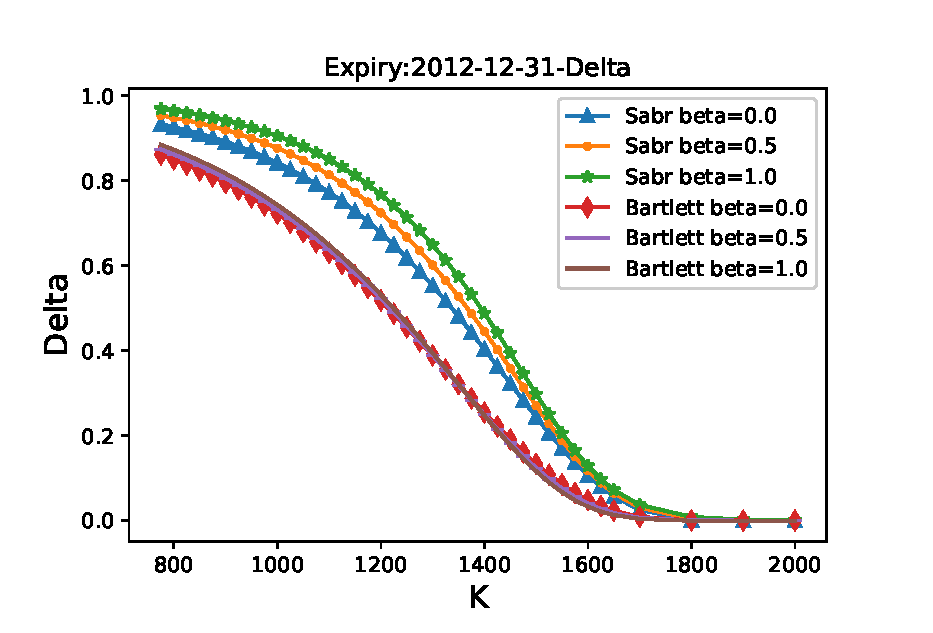
\includegraphics[width=\textwidth]{./figures/Bartlett}
        \caption{Comparing the original SABR delta $\delta^{SABR}_{t,T,K}$ and Bartlett delta  $\delta^{Bartlett}_{t,T,K}$ from SABR models calibrated with $\beta=0,\; 0.5, \;1.0$ on 2012-01-04 for S\&P500 index option. The computation of Bartlett delta  $\delta^{Bartlett}_{t,T,K}$ is more robust to the choice of $\beta$.}
        \label{fig:Bartlett}
    \end{figure}
    \item  Empirically, the Bartlett correction provides better hedging strategy. As an example, one can observe significant  hedging performance difference between $\delta^{Bartlett}_{t,T,K}$ and  $\delta^{SABR}_{t,T,K}$  on S\&P 500 index options. More specifically, we calibrate the SABR models on each trading date from Jan 1st 2007 to August 31st 2015 as discussed in section \ref{sec:pricing} with $\beta=1$ and note that here we calibrate SABR models separately for each expiry. And we compare the local hedging performance for all the traded options from Jan 1st 2007 to August 31st 2015.
    Following \cite{hulloptimal},  we use the Gain ratio below as the evaluating criteria of the hedging performance measure:
    \begin{equation}
    \textsc{Gain}=1-\frac{\sum_{i=1}^m \bigg(\Delta V^{mkt}_{t_i,T_i,K_i}-\delta_{t_i,T_i,K_i} ~ \Delta S_{t_i} \bigg)^2}{\sum_{i=1}^m \bigg(\Delta V^{mkt}_{t_i,T_i,K_i}-\delta^{BS}_{t_i,T_i,K_i} ~ \Delta S_{t_i} \bigg)^2}.
    \label{eq:Gain}
    \end{equation}
    where $m$ is the total number of data instances to be evaluated.  The $\delta^{BS}_{t_i,T_i,K_i}$ is the implied Black–Scholes delta, $\delta_{t_i,T_i,K_i}$  is the hedging position from the method under consideration,  e.g., SABR delta $\delta^{SABR}_{t_i,T_i,K_i}$,  MV delta $\delta^{MV}_{t_i,T_i,K_i}$, and  Bartlett delta $\delta^{Bartlett}_{t_i,T_i,K_i}$. $\Delta V^{mkt}_{t_i,T_i,K_i}$ and $\Delta S_{t_i}$
    are the changes in market option and underlying prices over a fixed time interval. Here we compare the \textbf{daily} local hedging risk with the daily changes of prices. The results are shown in Table \ref{table:Bartlett}:
    \begin{table}[htp!]
        \centering
        \begin{tabular}{|c|c|c|}
            \hline
            Method& SABR $\delta^{SABR}_{t,T,K}$ & Bartlett $\delta^{Bartlett}_{t,T,K}$\\
            Gain (\%) &-4.2 & 27.1 \\
            \hline
        \end{tabular}
        \caption{Daily local hedging risk comparison between original delta $\delta^{SABR}_{t,T,K}$ from SABR model and  $\delta^{Bartlett}_{t,T,K}$ from Bartlett correction. The performance is evaluated in terms of improvement over Black-Scholes delta on local hedging risk.}
        \label{table:Bartlett}
    \end{table}
    As we can see in Table \ref{table:Bartlett}, $\delta^{Bartlett}_{t,T,K}$ performs much better than $\delta^{SABR}_{t,T,K}$. What is more, $\delta^{SABR}_{t,T,K}$ actually performs worse than Black–Scholes delta $\delta^{BS}_{t,T,K}$ with implied volatility. The similar phenomenon has been observed in \cite{lassance2018comparison} where Heston and Heston-Nandi model performance worse than Black–Scholes delta $\delta^{BS}_{t,T,K}$ with implied volatility.  \textbf{The difference of the hedging performance between $\delta^{Bartlett}_{t,T,K}$ and $\delta^{SABR}_{t,T,K}$ is an example to illustrate how the unaccounted  pricing model parameter dependence on underlying asset affects the hedging performance. }Unfortunately, the pricing model parameter dependence often is not that easy to be accounted for as in SABR model with Bartlett correction.
\end{itemize}






Lastly, we introduce the corrective formula for minimum variance hedging  based on  SABR model implemented by  \citet{hulloptimal} . We use $\delta^{SV}$ to denote the minimum variance hedging  based on  SABR model from \cite{hulloptimal}. Let $\Delta F$ be a small changes in forward $F$, the  $\delta^{SV}$ is given by:
\begin{equation}
	\delta^{SV}_{t,T,K}=\frac{V_B(F_t+\Delta F,t,T,K,r;\sigma_B (F_t+\Delta F,t,T,K;\alpha,\beta,\nu,\rho))-V_B(F_t,t,T,K,r;\sigma_B (,t,T,K;\alpha,\beta,\nu,\rho))}{\Delta F}
	\label{eq:HullWhiteSabr}
\end{equation}
with $V_B$ be the Black pricing formula and $\sigma_B$ be the SABR implied volatility formula discussed in section \ref{sec:SABR}. 



\section{Motivation For Direct Nonparametric Data-Driven Hedging Models}
In the previous sections, we discuss the issue of parameter dependence and present several correction methods under Black–Scholes framework. Although the corrective formula   \eqref{eq:HullWhite}, \eqref{eq:HullWhiteLVF}, \eqref{eq:sabrV3}, and \eqref{eq:bartlett} adopt similar forms, the data-driven MV delta \eqref{eq:HullWhite} is significantly different from other corrective formula for the fact that it is based on historical data while \eqref{eq:HullWhiteLVF} ,\eqref{eq:sabrV3}, and \eqref{eq:bartlett} are based on pricing model calibrated to the spot options and underlying prices. \citet{hulloptimal} indicate that MV delta $\delta^{MV}_{t,T,K}$ estimated based on historical data performs better than $\delta^{LVF}_{t,T,K}$ and $\delta^{SV}_{t,T,K}$ estimated based on spot data. 

Our exploration on the data-driven models for hedging start roughly the same years as the work of \cite{hulloptimal} and we adopt the similar methodology as the MV delta where we learn a hedging position function from historical data. However, our explorations are motivated differently:
\begin{itemize}
    \item The hedging position  $\delta^{MV}_{t,T,K}$, $\delta^{LVF}_{t,T,K}$ and $\delta^{SV}_{t,T,K}$ proposed in \cite{hulloptimal} is to correct for the Black–Scholes implied volatility dependence on underlying asset. Specifically, \citet{hulloptimal} demonstrate how one can estimate the $\frac{\partial \sigma^{imp}}{\partial S}$ empirically.
    \item Noticing the pricing parameters dependence, we try to learn a hedging position directly from the market data.  We are not specifically trying to correct  parameters dependence for certain pricing models. We are trying to avoid it  by obtaining hedging position without a pricing model at all.
\end{itemize}
In addition, the data-driven models proposed in this thesis and MV delta are also different in the following ways:
\begin{itemize}
    \item \citet{hulloptimal} assume a quadratic form to account for the implied volatility dependence on the underlying asset within Black–Scholes framework.  The hedging position from our proposed data-driven models is  purely determined by market data with machine learning algorithms with no specific parametric form.
    \item The MV hedging model \eqref{eq:HullWhite} focuses on instantaneous hedging analysis  \eqref{eq:HE}. For discrete hedging, particularly when re-balancing is done infrequently, e.g., weekly or monthly, \eqref{eq:HullWhite}   may no longer be suitable. Our proposed models, which are not based on computing sensitivity of option pricing functions with regards to the underlying asset, can potentially improve the hedging results when the hedging is done less frequently.
    \item Our proposed data-driven models $\model$ and $\modelT$ can naturally include feature selection and feature extraction which can potentially improve the hedging performance.
    \item Our proposed data-driven model $\modelT$ is enhanced to deal with total hedging scenarios instead of focusing on reducing the instantaneous hedging risk as the   MV hedging model \eqref{eq:HullWhite}.
\end{itemize}
In the following chapters, we will start to formally describe the proposed hedging models and present numerical hedging performance comparison on both synthetic data and real market data.

\chapter{Data-Driven Kernel Learning Framework for Local Hedging Risk}
\label{sec:kernel}

In this chapter, we start the discussion on our proposed data-driven local hedging model from kernel learning framework. The data-driven kernel hedging model can be summarized as the following:
Assume we have $M$ data instances.  Each observation of a market option price  $V^{mkt}_{t_i,K_i,T_i}$ is uniquely associated with a triplet $\{t_i,T_i,K_i\}$, where $t_i$ is the trading time of the option price,  $K_i$ is the strike, and expiry $T_i$, $i=1,\ldots, M$.    The hedging position function is determined by the quadratic data-driven local risk minimization problem:
\[
\min ~\frac{1}{2M}\sum_{i=1}^{M} \left(\Delta S_{t_i} \delta(\vx_{t_i}^{T_i,K_i})- \Delta V^{mkt}_{t_i,K_i,T_i} \right)^2
\]
With $\Delta S_{t_i}$ and $\Delta V^{mkt}_{t_i,K_i,T_i}$ given in  \eqref{eq:DVDS} for a fixed time interval $\DT$.
The hedging position $\delta(\vx_{t_i}^{T_i,K_i})$ is given by a data-driven hedging function $\DKLs(\vx_{t}^{T,K};\valpha)$:
\[
	\delta(\vx_{t_i}^{T_i,K_i})=\DKLs(\vx_{t}^{T,K};\valpha)
\]
with  $\valpha$ being the parameters for the hedging functions and $\vx_{t}^{T,K}$ being the input features for the hedging function. Please note that $\valpha$ in this chapter is the parameter for the regularized kernel network to be learnt from data. The $\alpha$ in section \ref{sec:SABR} is the volatility for SABR. They are two unrelated terminologies.

From chapter \ref{sec:Background}, we have seen various challenges for hedging when the position is computed from the calibrated option value function. Since nonparametric option function estimation does not make specific assumptions and can potentially match option prices more accurately,  it is not unreasonable to  expect that this hedging challenge can potentially be addressed by reducing mis-specification using a data-driven approach to learn an option value function. Here we in this chapter we also discuss this approach and analyze its challenging for option hedging. Similar to discrete hedging under the parametric model, the hedging position can be computed by learning a nonparametric option value model and then determining hedging position from the partial derivatives. Indeed this is the approach adopted in \citep{hutchinson}.
In this chapters, we indicates that the issue of pricing model parameters dependence still exists even if one estimate the pricing model using a machine learning model with no assumption on the dynamic of the underlying asset movement. 

The organization of this chapter is as the following:
We discuss how one can compute a hedging positions from partial derivatives of the optimal regularized kernel functions in section \ref{sec:VF}. The proposed data-driven kernel hedging learning method is presented in section \ref{sec:KernelDirect}. In section \ref{sec:cross}, we discuss how cross-validation can be done efficiently for both kernel pricing and kernel hedging model. In section \ref{sec:Synexperiment}, we present experiments using synthetic data to illustrate the drawbacks of determining hedging position from partial derivative of pricing function estimated using machine learning algorithms and the effectiveness of data-driven direct kernel hedging functions.

\section{Regularized Kernel Pricing Model} 
\label{sec:RegularizedNW}
 Recognizing various challenges in the parametric financial modeling approach,
 nonparametric option pricing has also been studied. The nonparametric option value modeling approach has the distinctive advantage of not relying on specific assumptions about the underlying asset price dynamics. \citet{hutchinson} first propose a nonparametric data-driven approach to price and hedge European options using neural networks, radial basis functions, and projection pursuit regressions. Many other neural network methods for European option pricing have also been proposed, see, e.g., \citep{yao2000option,bennell2004black,gradojevic2009option,garcia2000pricing,malliaris1993neural}.


Although there are  quite a few studies on  nonparametric option pricing models, to our knowledge, there has been little research specifically focusing on discrete hedging using a nonparametric method. Even when the hedging problem is considered, e.g.,  \citep{hutchinson}, it is treated as a byproduct of obtaining a nonparametric  pricing function: The hedging position is obtained from the partial derivative of the option value function. \citet{hutchinson} show that, based on hedging errors on some simulated paths,  this indirect data-driven hedging approach can potentially be an effective alternative to the traditional parametric delta hedging methods.

In this section, we follow the methodology of \cite{hutchinson} and learn a data-driven option pricing model with the regularized kernel network. The hedging position is then given by the partial derivative of the option pricing model with regards to the underlying asset. Our goal is to learn a nonlinear option pricing function $V(\vx;\valpha)$  using a regularized kernel method \cite{evgeniou2000regularization}. 

Assume that we are given a positive definite kernel similarity
 $$
 \mathcal{K}(\vx, \vx^\prime) : \Real^{d} \times \Real^{d} \rightarrow  \Real,
 $$
 which captures  similarity between $\vx$ and $\vx^\prime$ implicitly in a high dimensional feature space.
 Assume that $\HK$ is the  \emph{Reproducing Kernel Hilbert Space} (RKHS) induced by the symmetric positive definite kernel function $ \mathcal{K}(\mathbf{x},\mathbf{y})$ and $\|f\|_{ \mathcal{K}}$ is the norm in RKHS.
 We have the following Representer Theorem \citep{wahba1990spline}:
\begin{thm}\label{pc:representer}
 (The Representer Theorem)
Let $\XS$ be a nonempty set and $k$ a positive definite real-valued kernel on $\XS \times \XS$ with the RKHS $\HK$.  Given the a training sample $
 \{\mathbf{x}_1, \mathbf{x}_2, \cdots, \mathbf{x}_M\} $, a strictly monotonically increasing real valued function $g:[0, \infty) \rightarrow \Real $,  and an arbitrary empirical risk function $E:\XS^M \rightarrow \Real $, then for any $f^* \in \HK$ satisfying
 \[
 f^*=\argmin_{f \in \HK} \;\;E\left(f(\mathbf{x}_1), f(\mathbf{x}_2), \cdots, f(\mathbf{x}_M)\right) + g( \|f\|_{\mathcal{K}})
 \]
 $f^*$ admits a representation of the form:
 \[
 f^*(\cdot)=\sum_{i=1}^M \widehat{\alpha}_i \mathcal{K}(\cdot,\mathbf{x}_i)
 \]
 with $\widehat{\alpha}_i \in \Real$  for all $1 \leq i \leq M$
\end{thm}

A regularized kernel regression problem can be formulated as
\begin{equation}
\min_{f \in \HK}\left(  \sum_{i=1}^M L(f(\vx_i))+\lambda_P \|f\|^2_{\mathcal{K}}\right)
\label{eq:indirect}
\end{equation}
where $L(\cdot)$ is a loss function.
The regularization parameter $\lambda_P>0$  can be determined based on cross validation.

Following the Representer Theorem,  e.g., \citep{wahba1990spline}, a solution of  \eqref{eq:indirect} has the form
\begin{equation}\label{kr1}
f(\mathbf{x})=\sum_{i=1}^M \widehat{\alpha}_i \mathcal{K}(\mathbf{x},\mathbf{x}_i)
\end{equation}
and the regularization term is given by
\begin{equation}\label{kr2}
\|f\|_{\mathcal{K}}^2=\sum_{i=1}^M \sum_{j=1}^M  \widehat{\alpha}_i \widehat{\alpha}_j \mathcal{K}(\mathbf{x}_i,\mathbf{x}_j).
\end{equation}


Assume that a set of $M$ training points $
 \{ (\vx_{t_1}^{T_1,K_1},V^{mkt}_{t_1,K_1,T_1}), \cdots, (\vx_{t_M}^{T_M,K_M},V^{mkt}_{t_M,K_M,T_M})\} $ are given, where
$
\vx_{t}^{T,K}  \in \Real^{d_l}
$ is the input feature for pricing the option with strike $K$ and expiry $T$ at time $t$ and  $V^{mkt}_{t,K,T}=\Vmkt(t,T,K)$ is the market option price at time $t$ with strike $K$ and expiry $T$.  Each data instance corresponds to a unique triplet $\{t,T,K\}$.
We can estimate an option value function $V(\vx;\mathbf{\valpha})$ based on the regularized kernel estimation \eqref{eq:indirect} with $\valpha=\{\widehat{\alpha}_1,\dots,\widehat{\alpha}_M\}$.


Using \eqref{kr1} and \eqref{kr2}, assuming quadratic loss, the option pricing function:
\[
	V(\vx_{t}^{T,K};\mathbf{\widehat{\alpha}})=\sum_{i=1}^N \widehat{\alpha}_i \mathcal{K}(\vx_{t}^{T,K},\vx_{t_i}^{T_i,K_i})
\] can be computed by solving
\begin{equation}
\min_{\mathbf{\widehat{\alpha}}} \left(  \sum_{i=1}^M \left( \Vmkt_{t_i,T_i,K_i}-\sum_{j=1}^M \widehat{\alpha}_j \mathcal{K}(\vx_{t_j}^{T_j,K_j},\vx_{t_i}^{T_i,K_i}) \right)^2+\lambda_P \sum_{i=1}^M\sum_{j=1}^M  \widehat{\alpha}_i \widehat{\alpha}_j \mathcal{K}(\vx_{t_j}^{T_j,K_j},\vx_{t_i}^{T_i,K_i})\right)
\label{eq:indirectf}
\end{equation}


For standard options, the universal RBF kernel
\begin{equation} \label{eq:RBF}
\mathcal{K}(\vx,\tilde{\vx})=e^{-\frac{\|\vx-\tilde{\vx}\|_2^2}{2 \rho^2}}
\end{equation}
is a reasonable kernel choice, since the option value function is very smooth, and
a suitable bandwidth $\rho$ is typically problem dependent and can be determined using cross validation.


\subsection{Indirect Hedging Positions From Kernel Pricing Functions} \label{sec:VF}

Assume that the one dimension  of the attribute vector $\vx_{t}^{T,K} \in \Real^{d_l}$ corresponds to the moneyness $S_t/K$ at time $t$ and other dimensions are not related to underlying prices. Then the delta hedging function option with strike $K$ and expiry $T$ at trading time $t$ is typically determined as:
\begin{equation}\label{eq:dV}
	\delta^{IKL}_{t,T,K}=
\frac{\partial V(\mathbf{x}_{t}^{T,K};\valpha)}{\partial S}=\sum_{i=1}^M  \widehat{\alpha}_i\frac{\partial \mathcal{K}(\mathbf{x}_{t}^{T,K},\vx_{t_i}^{T_i,K_i})}{\partial S} = \sum_{i=1}^M  \frac{\widehat{\alpha}_i}{K} \frac{\partial \mathcal{K}(\mathbf{x}_{t}^{T,K},\vx_{t_i}^{T_i,K_i})}{\partial S/K} 
\end{equation}
\citet{hutchinson} demonstrate that this nonparametric hedging approach,  using the partial derivative of a nonparametric pricing function learned from historical market data, can be a useful alternative for option hedging.

However, using \eqref{eq:dV} as the hedging position similarly does not minimize variance of hedge risk in general and the challenge in accounting for parameter dependence on the underlying remains. We can see that from the  following arguments. We made an unrealistic assumption that the estimated kernel function $V(\mathbf{x}_{t}^{T,K};\valpha)$ matches the target market option price exactly, i.e.,
$$
V(\mathbf{x}_{t}^{T,K};\valpha) = \Vmkt_{t,T,K}
$$
and $$\frac{d V}{d S}(\mathbf{x}_{t}^{T,K};\valpha)=\frac{d  \Vmkt}{d S}$$
Then we have:
$$
\frac{d V}{d S}(\mathbf{x}_{t}^{T,K};\valpha)=\sum_{i=1}^M \widehat{\alpha}_i \frac{\partial \mathcal{K}(\mathbf{x}_{t}^{T,K},\vx_{t_i}^{T_i,K_i})}{\partial S} + \sum_{i=1}^M \frac{\partial \widehat{\alpha}_i}{\partial S}\mathcal{K}(\vx,\vx_i)=\frac{d \Vmkt}{d S}
$$
Hence in general
$$
\frac{\partial \widehat{\alpha}_i}{\partial S} \neq 0
$$
unless
\begin{equation}\label{eq:dep}
\frac{\partial V}{\partial S}(\vx_{t}^{T,K};\valpha) = \frac{d  \Vmkt}{d S}.
\end{equation}
However there is no reason that a solution of the regression problem (\ref{eq:indirectf}) should satisfy \eqref{eq:dep}. Consequently it is similarly difficult to account for all dependence from $\valpha$ on the underlying asset, even infinitesimally, in the estimated kernel model.



Furthermore, error magnification can happen by deriving the hedging position from a estimated kernel function. In general, the estimated kernel pricing function $V(\mathbf{x}_{t}^{T,K};\valpha)$ can not match the all the target market option prices exactly and the  estimated kernel pricing function inevitably will have prediction error when used to predict the price of unobserved testing data instances. The calibration error and prediction can potentially increase the hedging error when using the $\frac{\partial V}{\partial S}(\vx_{t}^{T,K};\valpha)$ as the hedging position.


\section{Regularized Kernel Hedging Model}
\label{sec:KernelDirect}
Let us again assume that a set of $M$ training points 
\[
 \left\{ (\vx_{t_1}^{T_1,K_1},\Delta V^{mkt}_{t_1,K_1,T_1},\Delta \Smkt_{t_1}), \cdots, (\vx_{t_M}^{T_M,K_M},\Delta V^{mkt}_{t_M,K_M,T_M},\Delta \Smkt_{t_M})\right\} \]
 are given, where
$
\vx_{t}^{T,K}  \in \Real^{d_l}
$ is the input feature for \textbf{hedging} the option with strike $K$ and expiry $T$ at time $t$. The $\Delta V^{mkt}_{t,K,T}$ is the change of  market option price at time $t$ with strike $K$ and expiry $T$ over a fixed time intervel $\DT$, e.g., daily, weekly, or monthly. The $\Delta \Smkt_{t}$ is the change of  underling price at time $t$ over a fixed time intervel $\DT$ over the same $\DT$. 
$\Delta V^{mkt}_{t,K,T}$ and  $\Delta \Smkt_{t}$  are given by
equation \eqref{eq:DVDS}.
Again, each data instance corresponds to a unique triplet $\{t,T,K\}$.

We can estimate an option hedging function $\delta(\vx_{t}^{T,K};\mathbf{\valpha})$ based on the regularized kernel network with $\valpha=\{\widehat{\alpha}_1,\dots,\widehat{\alpha}_M\}$. The empirical loss function is chosen to correspond to the square of discrete local hedging risk in section \ref{sec:DiscreteHedgingCriteria}, i.e., 
\begin{equation}\label{eq:HR}
L\left(\delta(\vx_{t}^{T,K};\valpha)\right)=\left(\Delta V^{mkt}_{t,K,T}-\DS_{t} \delta(\vx_{t}^{T,K};\valpha)\right)^2.
\end{equation}
The hedging position function $\delta(\vx_{t}^{T,K};\valpha)$  can be estimated from  the regularized optimization below:
\begin{equation} \label{fhedge}
\min_{\delta \in \HK}\left\{\sum_{i=1}^M L\left(\delta(\vx_{t_i}^{T_i,K_i};\valpha)\right)^2+\lambda_P \|\delta\|^2_\mathcal{K}\right\}
\end{equation}
Note that the Representer Theorem still holds for \eqref{fhedge}.
Using the Representer Theorem \eqref{kr1} and \eqref{kr2}, \eqref{eq:directf} can be computed by solving the following convex quadratic minimization,
\begin{equation}
	\min_{\mathbf{\valpha}} \left(  \sum_{i=1}^M \left( \Delta \Vmkt_{t_i,T_i,K_i}-\Delta S_{t_i} \sum_{j=1}^M \widehat{\alpha}_j \mathcal{K}(\vx_{t_j}^{T_j,K_j},\vx_{t_i}^{T_i,K_i}) \right)^2+\lambda_P \sum_{i=1}^M\sum_{j=1}^M  \widehat{\alpha}_i \widehat{\alpha}_j \mathcal{K}(\vx_{t_j}^{T_j,K_j},\vx_{t_i}^{T_i,K_i})\right)
	\label{eq:directf}
\end{equation}


The loss function for the hedging function in the proposed formulation \eqref{fhedge}
directly corresponds to the sum of square of local hedging risk for a discrete $\DT$-time period. In addition the hedge function is the solution of the optimization problem  and there is no potential error magnification through partial derivative computation. We avoid the pricing model parameters dependence on underlying asset by not computing a prcing model at all.




Since at the expiry the delta of the payoff function is a discontinuous step function, the  delta hedging function of an option changes quickly as the underlying changes near the expiry.
Consequently we choose to use a spline kernel function \citep{vapnik1998statistical} for the hedging function estimation.
The explicit expression for the spline kernel with order $O_d$  for the one-dimensional case is :
\[
\mathcal{K}(x,y)=\sum_{r=0}^{O_d} \frac{\binom{O_d}{r}}{2 O_d-r+1} min(x,y)^{2 O_d-r+1}|x-y|^r +\sum_{r=0}^{O_d} x^ry^r
\]

For multidimensional data, the spline kernel is the product of one-dimensional spline kernel functions with regard to each dimension. Interested readers can referred to \citep{vapnik1998statistical} for more details. The major benefit of using the spline kernel over the gaussian kernel  is that spline kernel does not have a hyperparameter to be tuned while  gaussian kernel has  a bandwidth parameter to be tuned by cross-validation which is often costly. In this thesis, we majorly use spline kernel and, in section 
\ref{sec:Synexperiment}, we will show that spline kernel performs better or equally well when compared with gaussian kernel.  In the latter discussion, we denote $\delta^{DKL}_{t,T,K}= \delta(\vx_{t}^{T,K};\mathbf{\valpha})$ as the hedging position form the directly kernel hedging model.


\section{Cross Validation} \label{sec:cross}
 For our data-driven approach, we need to select an appropriate penalty $\lambda_P$ to control the model complexity. Cross-validation (CV) is a commonly used method for the performance estimation and model selection for the learning algorithms. For example, the Leave-One-Out Cross-Validation (LOOCV) computes the output for each data instance using parameters trained on the remaining data instances. For the regularized kernel methods, we can compute the CV error efficiently without retraining the model in each CV round.


Recall that, for the regularized network or pricing model, the minimization problem is
\[
\min_{\mathbf{\valpha}} \left(  \sum_{i=1}^M \left( \Vmkt_{t_i,T_i,K_i}-\sum_{j=1}^M \widehat{\alpha}_j \mathcal{K}(\vx_{t_j}^{T_j,K_j},\vx_{t_i}^{T_i,K_i}) \right)^2+\lambda_P \sum_{i=1}^M\sum_{j=1}^M  \widehat{\alpha}_i \widehat{\alpha}_j \mathcal{K}(\vx_{t_j}^{T_j,K_j},\vx_{t_i}^{T_i,K_i})\right)
 \]
Let $\vK$ be the kernel matrix with $\vK_{ij}=\mathcal{K}(\mathbf{x}_i,\mathbf{x}_j)$. (Note $\vK$ here denotes the kernel matrix which should not be confused with the strike $K$.) Problem \eqref{eq:indirect} can be rewritten in matrix form:
\begin{equation}
\min_{\valpha \in \Real^M} \; ( \vK \valpha - \vecVmkt)^T ( \vK \valpha -\vecVmkt)+ \lambda_P \valpha^T\vK\valpha
\label{eq:CV2}
\end{equation}
with
\[
	\vecVmkt=\{
	\Vmkt_{t_1,T_1,K_1},\dots,	\Vmkt_{t_M,T_M,K_M}
	\}	\;\;\;,\;\;\; \valpha=\{\widehat{\alpha}_1,\dots,\widehat{\alpha}_M\}
\]
The solution to \eqref{eq:CV2} is:
\[
\valpha  =(\vK+\lambda_P \pmb{I})^{-1}\vecVmkt
\]
Given the eigen-decomposition $\vK=\pmb{Q} \pmb{\Lambda} \pmb{Q}^T$, we can easily see that:
\begin{equation}\label{eq:eig}
(\vK+\lambda_P \pmb{I})^{-1}=\pmb{Q}(\pmb{\Lambda}+\lambda_P \pmb{I})^{-1} \pmb{Q}^T
\end{equation}
Because $(\pmb{\Lambda}+\lambda_P I)$ is a diagonal matrix, given the eigen-decomposition $\vK=\pmb{Q} \pmb{\Lambda} \pmb{Q}^T$, we can get different solutions to \eqref{eq:CV2}  as $\lambda_P$ varies in $O(M^2)$.

Let $V(\vx_{t_j}^{T_j,K_j}; \valpha)$ be the output for data instance $j$ when regularized kernel methods \eqref{eq:indirectf} is trained on all training data instances. Let $V^l(\vx_{t_j}^{T_j,K_j}; \valpha^l)$  be the output for data instance $j$ when regularized kernel methods \eqref{eq:indirectf} is trained on all training data instances except $\vx_{t_l}^{T_l,K_l}$. 
Let $\vecVmkt^l=\{\vecVmkt^l_1,\vecVmkt^l_2,\cdots,\vecVmkt^l_M\}$ be the vector where $\vecVmkt^l_{j} = \Vmkt_{t_j,T_j,K_j}$ for $j \neq l$ and $\vecVmkt^l_l = V^l(\vx_{t_l}^{T_l,K_l}; \valpha^l)$. Since $V^l(\cdot; \valpha^l)$ is the model trained on all example except $\vx_{t_l}^{T_l,K_l}$ , it is easy to see that $V^l(\cdot; \valpha^l)$  minimizes
\begin{equation}
\min_{\valpha \in \Real^M} \; ( \vK \valpha - \vecVmkt^l)^T ( \vK \valpha -\vecVmkt^l)+ \lambda_P \valpha^T\vK\valpha
\label{eq:CV3}
\end{equation}
The solution to \eqref{eq:CV3} is:
\[
\valpha^l  =(\vK+\lambda_P \pmb{I})^{-1}\vecVmkt^l
\]
Let $\pmb{B}=\vK (\vK+\lambda_P \pmb{I})^{-1}$, therefore, we have 
\[\pmb{B}\vecVmkt=\{
	V(\vx_{t_1}^{T_1,K_1}; \valpha),
	\dots,
	V(\vx_{t_M}^{T_M,K_M}; \valpha)
	\}
\]
We can easily show that:
\[
	V^l(\vx_{t}^{T,K}; \valpha^l)-V(\vx_{t}^{T,K}; \valpha)=\sum_{i=1}^M B_{li}(\vecVmkt_i^l-\vecVmkt_i)=B_{ll}(V^l(\vx_{t_l}^{T_l,K_l}; \valpha^l)-\vecVmkt_l)=B_{ll}(V^l(\vx_{t_l}^{T_l,K_l}; \valpha^l)-\Vmkt_{t_l,T_l,K_l})
\]
Thus,
\begin{equation} \label{eq:fastCV}
	V^l(\vx_{t_l}^{T_l,K_l}; \valpha^l)=
	\frac{V(\vx_{t_l}^{T_l,K_l}; \valpha^l)-B_{ll}\Vmkt_{t_l,T_l,K_l}}
	{1-B_{ll}}
\end{equation}
Therefore, we can get the $V^l(\vx_{t_l}^{T_l,K_l}; \valpha^l)$  without actually retraining the model. The leave-one-out estimations for all data instance are:
\begin{equation} \label{eq:fastCV2}
\vecVmkt_{loo}=(I-B_{LL})^{-1}(B\vecVmkt-B_{LL}\vecVmkt)
\end{equation}
and the leave-one-out errors for all data instance are:
\begin{equation} \label{eq:fastCV3}
\vecVmkt-\vecVmkt_{loo}=\vecVmkt-(\pmb{I}-B_{LL})^{-1}(\pmb{B}\vecVmkt-\pmb{B}_{LL}\vecVmkt)=(I-\pmb{B}_{LL})^{-1}(\vecVmkt-\pmb{B}\vecVmkt)
\end{equation}
where $B_{LL}$ is a diagonal matrix with $B_{ii},\;\; i=1,\dots,M$ on its diagonal.

We can further simplify the expression by noting the fact that:
\[\begin{split}
\pmb{B}&=\vK (\vK+\lambda_P \pmb{I})^{-1} \\
       &=\pmb{Q}\pmb{\Lambda}(\pmb{\Lambda}+\lambda_P \pmb{I})^{-1} \pmb{Q}^T\\
       &=\pmb{Q}(\pmb{\Lambda}+\lambda_P \pmb{I}-\lambda_P \pmb{I})(\pmb{\Lambda}+\lambda_P \pmb{I})^{-1} \pmb{Q}^T\\
       &= \pmb{I}-\lambda_P Q (\pmb{\Lambda}+\lambda_P \pmb{I})^{-1} \pmb{Q}^T=\pmb{I} -\lambda_P  (\vK+\lambda_P \pmb{I})^{-1}
  \end{split}
\]
Therefore, we can get:
\[
(\pmb{I}-\pmb{B}_{LL})=diag(\pmb{I}-\pmb{B})=\lambda_P \; diag((\vK+\lambda_P \pmb{I})^{-1})
\]
\[
\vecVmkt-B\vecVmkt=\lambda_P (\vK+\lambda_P \pmb{I})^{-1} \vecVmkt =\lambda_P \valpha
\]
Finally, we can get:
\begin{equation}  \label{eq:fastCV4}
\vecVmkt-\vecVmkt_{loo}=diag((\vK+\lambda_P \pmb{I})^{-1})^{-1} \valpha
\end{equation}

Given the eigen-decomposition $\vK=\pmb{Q} \pmb{\Lambda} \pmb{Q}^T$, we can compute  $\valpha$ as $\lambda_P$ varies in $O(M^2)$. Similarly, given the eigen-decomposition $\vK=\pmb{Q} \pmb{\Lambda} \pmb{Q}^T$, we can compute the diagonal of $(\vK+\lambda_P \pmb{I})^{-1}$ in $O(M^2)$. Then  using \eqref{eq:fastCV4}, the LOOCV errors can be computed in $O(M^2)$.  It can been further shown \cite{pahikkala2006fast} that, given the eigen-decomposition $\vK=\pmb{Q} \pmb{\Lambda} \pmb{Q}^T$, the computational complexity for the $n$-fold cross-validation ($n$FCV) is $O(M^3/n)$. Interested readers can referred to \citep{pahikkala2006fast, wahba1990spline} for more details.

Let $\Delta \vecVmkt=\{\Delta \Vmkt_{t_1,T_1,K_1},\cdots,\Delta \Vmkt_{t_M,T_M,K_M}\}$ and  let $\pmb{D}$ be a diagonal matrix with $D_{ii}=\Delta S_{t_i}. \;i=1,\cdots,M.$ on its diagonal.
Similarly, we can rewrite  the minimization problem \eqref{eq:directf} in matrix form:
\begin{equation}
\min_{\valpha \in \Real^m} \; ( \pmb{D} \vK \valpha - \Delta \vecVmkt)^T (\pmb{D}  \vK \valpha -\Delta \vecVmkt)+ \lambda_P \valpha^T\vK\valpha
\label{eq:directfM}
\end{equation}
Let $\widetilde{\vK}=\pmb{D}\vK$, the solution to \eqref{eq:directfM} can be obtained by:
\[
\valpha = (\widetilde{\vK}^T\widetilde{\vK}  + \lambda_P \vK)^{-1} \widetilde{\vK}^T \Delta \vecVmkt
\]
Unfortunately, we can not directly use the fast cross validation algorithms from \cite{pahikkala2006fast, wahba1990spline} for the minimization problem \eqref{eq:directfM}.
Because $(\pmb{\widetilde{K}}^T\pmb{\widetilde{K}}  + \lambda_P \vK)^{-1}$ can not be easily inverted in $O(M^2)$ as $\lambda_P$ varies.

However if we change the penalty term for \eqref{eq:directfM} from $\lambda_P \valpha^T\vK\valpha$ to $\lambda_P \valpha^T\valpha$, the minimization problem becomes:
\begin{equation}
\min_{\valpha \in \Real^m} \; ( \pmb{D} \vK \valpha - \Delta\vV)^T (\pmb{D}  \vK \valpha -\Delta\vV)+ \lambda_P \valpha^T\valpha
\label{eq:directfMV2}
\end{equation}
The solution to \eqref{eq:directfMV2} can be obtained by:
\[
\valpha = (\widetilde{\vK}^T\widetilde{\vK}  + \lambda_P \pmb{I})^{-1} \widetilde{\vK}^T \Delta \vecVmkt
\]
Utilizing the ideas from \cite{pahikkala2006fast, wahba1990spline}, we can similarly show that,  given the singular value decomposition $\pmb{\widetilde{K}}=\pmb{U} \pmb{\Sigma} \pmb{V}^T$, for the problem \eqref{eq:directfMV2},  the computational complexity for the LOOCV is still $O(M^2)$ and the computational complexity for the $n$FCV is still $O(M^3/n)$. In practice, changing the penalty term from $\lambda_P \valpha^T\vK\valpha$ to $\lambda_P \valpha^T\valpha$ will not affect the actual performance too much. Therefore, in order to improve the computation efficiency for the direct data driven approach, we are solving the problem \eqref{eq:directfMV2}.






\section{Comparison using synthetic data}\label{sec:Synexperiment}
Following the S\&P 500  market option specifications in \citep{hull2006options},  we first synthetically generate option data assuming that the underlying price follows a Heston model \citep{heston1993closed}.
We  compare hedging effectiveness of direct hedging function learning \eqref{fhedge}  and indirect hedging function estimation  \eqref{eq:indirectf}. In addition, we compare their performance to that of using  analytic delta under the  Heston model, which can be regarded as a best case benchmark, at least for daily hedging. Note that there is no model mis-specification  for the underlying price in this synthetic case.

The experiments in the this section is to demonstrate the following aspects:
\begin{itemize}
\item Computing the hedging position as the partial derivative of an nonparametric option pricing model with regards to underlying asset still suffers from the issue of parameter dependence on underlying asset.
\item The hedging position directly learnt from data as in \eqref{eq:directf} can be very close to the  best case benchmark in daily hedging.
\item The hedging position directly learnt from data using spline kernel performs better when compared with gaussian kernel.
\end{itemize}

Since the loss function is  quadratic, solutions to \eqref{fhedge} and \eqref{eq:indirectf}
can be easily computed from linear equation solvers.
In addition we also compare hedging performance using a RBF kernel \eqref{eq:RBF} versus a spline kernel.
Specifically, using the generated synthetic data, we compare here hedging performance  of the following hedging computation methods:
 \begin{itemize}
 \item  $\delta^{BS}_{t,T,K}$:  implied  volatility BS delta
 \item $\delta^{Heston}_{t,T,K}$:   analytical Heston delta
 \item $\DKLs$ : direct learning a spline kernel hedging  function based on \eqref{fhedge}
 \item $\DKLg$ : directly learning a RBF kernel hedging  function directly based on \eqref{fhedge}
 \item ${\IKLs}$: determining hedging position indirectly  as the partial derivative \eqref{eq:dV} of the  option value function   estimated from \eqref{eq:indirectf} using a spline kernel

\item ${\IKLg}$: determining hedging position indirectly  as the partial derivative \eqref{eq:dV} of the  option value function   estimated from \eqref{eq:indirectf} using a RBF kernel

\end{itemize}

Training data consists of simulated daily underlying price $S_t$ for two years\footnote{We assume that there are 252 trading days in a year.}, $t=1,\cdots, 2\times 252$, assuming a  risk-neutral Heston model below:
\[
	\begin{split}
	dS&=(r-q) S dt + \sqrt{\Upsilon} S \hat{dW}\\
	d\Upsilon&=\kappa^*(\overline{\Upsilon}^*-\Upsilon)dt+\eta \sqrt{\Upsilon}\hat{dZ}\\
	E[\hat{dZ}\hat{dW}]&=\rho dt
	\end{split}
\]
In addition,  a vector of simulated (traded)  market call option prices  are  generated,  on each day $t$, with different strikes and time to expiry, following  the CBOE specifications of stock options described in  \cite{hull2006options}.
 The option prices $\Vmkt$ are  computed using  the analytical option 
 formula \eqref{eq:hestonPrice} under the Heston model \citep{heston1993closed} in section \ref{sec:heston} ,
 using the the parameters  from \citep{bakshi1997empirical}, which are given in Table \ref{para}. In other words, we assume in this section:
 \[
\Vmkt(t,T,K)=V_{Heston}(S_t,t,T,K,r,q;\Upsilon,\kappa^*,\overline{\Upsilon}^*,\eta,\rho)
 \]

 Please note that the heston delta position under this synthetic scenarios does not have the parameter dependence issue, since for the synthetic case all heston parameter is fixed, and can be used as the benchmark.
 \[
	 \delta^{Heston}_{t,T,K}=\frac{ \partial V_{Heston}(S_t,t,T,K,r,q;\Upsilon,\kappa^*,\overline{\Upsilon}^*,\eta,\rho)}{\partial S}=\frac{d \Vmkt}{d S}
 \] 
 The Black-Scholes delta position from implied volatility still has the the issue of implied volatility depending on underlying asset:
 \[
	 \delta^{BS}_{t,T,K}=\frac{ \partial V_{BS}(S_t,t,T,K,r,q;\sigma^{imp}_{t,T,K})}{\partial S} \neq \frac{d \Vmkt}{d S}
 \] 
 where $\sigma^{imp}_{t,T,K}$ is the volatility that equals Black–Scholes price and Heston price
 \[
	 V_{BS}(S_t,t,T,K,r,q;\sigma^{imp}_{t,T,K})=V_{Heston}(S_t,t,T,K,r,q;\Upsilon,\kappa^*,\overline{\Upsilon}^*,\eta,\rho)
 \]

 \begin{table}[htp!]
\begin{center}
\begin{tabular}{|c|c|c|c|c|c|c|c|}
\hline
 $r$ &$q$& $\overline{\Upsilon}^*$  & $\kappa^*$ & $\eta$ & $\rho$ & $S_0$ & $\Upsilon_0$  \\ \hline
 0.02&0.0&0.04                  & 1.15   & 0.39  & -0.64 & 100 &0.04 \\    \hline
\end{tabular}
\end{center}

\caption{Parameters for the Heston model. This set of parameters is used to generate synthetic experiments for demonstrating the effectiveness of $\DKLs$ on local hedging.}
\label{para}
\end{table}



Testing data consists of 100 daily underlying price paths and corresponding option prices, spanning a six month period. The Heston parameter is still specified as in Table \ref{para}. We report average performance measures over 10 random training-test-data sets generated as described. \footnote{Following CBOE option specification rules, the size of a training or testing data set can vary slightly for each simulation run.}



We train a regularized option price kernel model for the indirect hedging $\IKLs$ and $\IKLg$. For $\IKLs$ and $\IKLg$,
the hedging position is  the partial derivative of the estimated pricing function  \eqref{eq:dV},  as in \citep{hutchinson}. We note that the simulation hedging analysis in \cite{hutchinson} considers only the Black–Scholes model and the results in \citep{hutchinson} indicate that a lower hedging error can be achieved on a subset of simulated paths.


Following a common practice, we use the standard deviation of the pairwise Euclidean distance of the training data as the bandwidth $\rho$ for the RBF kernel. The regularization parameter $\lambda_P$  is however selected using a 5-fold cross-validation. We also consider weekly hedging and monthly hedging, which correspond to hedging over a 5-business-days period and 20-business-days period respectively.

To investigate impact of the feature choice,  we evaluate hedging performance using
\begin{itemize}
\item
$\text{Feature Set \#1} = \{\textsc{moneyness}\; (S_t/K),\;\;\textsc{time-to-expiry}\; (T-t)\}$.
\item
$\text{Feature Set \#2} = \{\textsc{moneyness} \;(S_t/K),\;\;\textsc{time-to-expiry} \;(T-t) ,\;\;~ \delta^{BS}_{t,T,K}\}$.
\end{itemize}
In the second feature set,  the Black–Scholes delta $\delta^{BS}_{t,T,K}$ using the implied volatility  is used as an additional feature in determining the hedging position. 

Let the number of data instances to be evaluated be $m$.
We have the profit and loss \eqref{eq:localPL} of the local hedging portfolio in section \ref{sec:DiscreteLocalRisk} over the fixed time interval $\DT$ for each data instance, which corresponds to a unique triplet $\{t,T,K\}$:
\[
	\Delta P^{H}_{t,T,K}=\Delta \Smkt_{t} \delta_{t,T,K} -\Delta V^{mkt}_{t,K,T}
\]
where $\delta_{t,T,K}$ is the hedging position from different approaches, e.g., Black–Scholes delta $\delta^{BS}_{t,T,K}$, Heston delta $\delta^{Heston}_{t,T,K}$, direct data-driven hedging position $\delta^{DKL}_{t,T,K}$, and  indirect data-driven hedging position$\delta^{IKL}_{t,T,K}$.
We evaluate the performance in four different ways:
\begin{enumerate}
	\item Gain \eqref{eq:Gain} over Black-Scholes $\delta^{BS}_{t,T,K}$ as in \cite{hulloptimal}.
	\item The mean absolute value of $\Delta P^{H}_{t,T,K}$
	\[
		\MeanAbs=\frac{1}{m}\sum_{i=1}^m |\Delta P_{H}(t_i,T_i,K_i)|
	\]

	\item The 95\% Value-at-Risk (VaR) of $\{\Delta P_{H}(t_i,T_i,K_i)| i=1,\dots, m\}$
	\item The 95\% Conditional-Value-at-Risk (CVaR) of $\{\Delta P_{H}(t_i,T_i,K_i)| i=1,\dots, m\}$
\end{enumerate}

\subsubsection{Feature Set \#1:$ \{\textsc{moneyness} \;(S_t/K),\;\;\textsc{time-to-expiry} \;(T-t)\}$}
For the synthetic data, it is known that the option price is a function of
 the moneyness $ \frac{S}{K}$ and time to expiry $T-t$, which are the attributes $\vx_{t}^{T,K}$ in Feature Set \#1. Table \ref{Daily}, \ref{Weekly} and \ref{Monthly} report results for daily, weekly, and monthly hedging respectively.

 \begin{table}[htp!]
\begin{center}
\begin{threeparttable}
\begin{tabular}{|l|r c c c c|}
\hline
Method & Gain (\%)& $\MeanAbs$ & Std& VaR & CVaR   \\ \hline
$\Del$ & 0.0 & 0.185 & 0.286 & 0.380 & 0.574 \\
$\IKLg$  & -3.3 & 0.171 & 0.291 & 0.356 & 0.566 \\
$\IKLs$  & -183.3 & 0.291 & 0.482 & 0.669 & 1.105 \\
$\DKLg$  & 63.1 & 0.120 & 0.174 & 0.251 & 0.352 \\
$\DKLs$  & \textbf{64.9} & \textbf{0.121} & \textbf{0.170} & \textbf{0.255} & \textbf{0.345} \\
$\Heston$ & 63.6 & 0.121 & 0.173 & 0.266 & 0.360 \\
%$\DKLgd$  & 62.3 & 0.114 & 0.176 & 0.238 & 0.349 \\
%$\DKLsd$  & \textbf{70.9} &\textbf{ 0.110 }& \textbf{0.154} & \textbf{0.234} & \textbf{0.322} \\
\hline
\end{tabular}
\caption{Daily hedging comparison on synthetic experiments between various hedging strategies. The hedging performance is evaluated in terms of local hedging risk.}
\label{Daily}
 \begin{tablenotes}
    \small
  \item[1] FS \#1: $\vx=\{\textsc{moneyness,~time-to-expiry}\}$
  \item[2] Bold entry indicating best Gain
  \end{tablenotes}
  \end{threeparttable}
\end{center}
\end{table}

\begin{table}[htp!]
\begin{center}
\begin{threeparttable}
%\begin{tabular}{|l|r|c|c|c|c|}
\begin{tabular}{|l|r c c c c|}
\hline
Method & Gain (\%) & $\MeanAbs$ & Std& VaR & CVaR   \\ \hline
$\Del$ & 0.0 & 0.414 & 0.620 & 0.776 & 1.009 \\
$\IKLg$  & -197.6 & 0.406 & 1.070 & 0.741 & 1.254 \\
$\IKLs$  & -94.7 & 0.548 & 0.866 & 1.114 & 1.738 \\
$\DKLg$  & 47.0 & 0.312 & 0.451 & 0.620 & 0.825 \\
$\DKLs$  & \textbf{50.8} & \textbf{0.312} & \textbf{0.435} & \textbf{0.622} & \textbf{0.797} \\
$\Heston$ & 45.7 & 0.319 & 0.456 & 0.651 & 0.840 \\
\hline
\end{tabular}
\caption{Weekly hedging comparison on synthetic experiments between various hedging strategies. The hedging performance is evaluated in terms of local hedging risk.}
\label{Weekly}
 \begin{tablenotes}
    \small
  \item[1] FS \#1: $\vx=\{\textsc{moneyness,~time-to-expiry}\}$
  \item[2] Bold entry indicating best Gain
  \end{tablenotes}
  \end{threeparttable}
\end{center}
\end{table}


\begin{table}[htp!]
\begin{center}
\begin{threeparttable}
\begin{tabular}{|l|r c c c c|}
\hline
Method & Gain (\%)& $\MeanAbs$ & Std& VaR & CVaR   \\ \hline
$\Del$ & 0.0 & 0.941 & 1.484 & 1.516 & 1.808 \\
$\IKLg$  & 1.0 & 0.888 & 1.470 & 1.516 & 1.829 \\
$\IKLs$  & -36.9 & 1.135 & 1.729 & 2.033 & 2.894 \\
$\DKLg$  & 33.6 & 0.860 & 1.181 & 1.612 & 1.949 \\
$\DKLs$  & {35.4} & {0.858} & {1.165} & {1.610} & {1.922} \\
$\Heston$ & \textbf{38.7} & \textbf{0.814} & \textbf{1.136} & \textbf{1.544} & \textbf{1.829} \\
\hline
\end{tabular}
\caption{Monthly hedging comparison on synthetic experiments between various hedging strategies. The hedging performance is evaluated in terms of local hedging risk.}
\label{Monthly}
\begin{tablenotes}
    \small
  \item[1] FS \#1: $\vx=\{\textsc{moneyness,~time-to-expiry}\}$
  \item[2] Bold entry indicating best Gain
  \end{tablenotes}
  \end{threeparttable}
  \end{center}
\end{table}


Table \ref{Daily} and \ref{Weekly}  demonstrate that the direct hedging function learning $\DKLs$ \& $\DKLg$  significantly outperform the indirect hedging learning $\IKLs$ \& $\IKLg$ in Gain and different risk measures considered. Indeed, $\DKLs$ \& $\DKLg$ slightly outperform the benchmark of using the analytic Heston delta.
The indirect hedging function learning performs more poorly than the implied BS delta hedging. In addition,  the spline kernel performs better than the RBF kernel (with the standard deviation as the bandwidth parameter). The RBF kernel yields larger risk measures and smaller Gain  for both the direct and indirect hedging learning methods.

Table \ref{Monthly} reports hedging comparison for monthly hedging. We  observe that  $\DKLs$ \& $\DKLg$  significantly outperform the indirect hedging learning $\IKLs$ \& $\IKLg$ in  Gain and various risk measures. In addition, $\DKLs$ \& $\DKLg$ continue to achieve enhanced performance over $\Del$, with the spline kernel $\DKLs$ yielding better results than $\DKLg$.
Not surprisingly, hedging performance of each method also deteriorates as the length of the hedging period increases,  with larger mean absolute hedging error and larger standard deviation for monthly hedging than for daily and weekly hedging.

Table \ref{Monthly} also illustrates that, unlike daily and weekly hedging, $\DKLs$ \& $\DKLg$ slightly underperform the analytic Heston delta benchmark  for monthly hedging.
Given that the analytic delta is for instantaneous hedging while the direct hedging learning $\DKLs$ minimizes quadratic hedging error, one would expect better performance from the direct hedging learning $\DKLs$. We suspect that this is due to the effect of the specific combination of choices of features and kernel. Next we show that,  with a different feature set,   performance of direct hedging is improved, which suggests the possibility of surpassing  analytic Heston delta benchmark, using a more suitable feature set, for a longer period hedging.


\subsubsection{Feature Set \#2: $ \{\textsc{moneyness} \;(S_t/K),\;\;\textsc{time-to-expiry} \;(T-t) ,\;\;~ \delta^{BS}_{t,T,K}\}$}
We add the Black–Scholes delta $\delta^{BS}_{t,T,K}$ using the implied volatility as an additional feature in the direct hedging learning, since \citet{hulloptimal} indicate that a better minimum  variance hedge can be calculated based on the implied volatility delta.  Table \ref{DailyD}, \ref{WeeklyD}, and \ref{MonthlyD}
present hedging results for  $\DKLs$ \& $\DKLg$ for  $\{\textsc{moneyness} \;(S_t/K),\;\;\textsc{time-to-expiry} \;(T-t) ,\;\;~ \delta^{BS}_{t,T,K}\}$. For clarity, we also include the results for FS \#1 $\{\textsc{moneyness} \;(S_t/K),\;\;\textsc{time-to-expiry} \;(T-t) \}$ and Heston delta for ease of comparison.

\begin{table}[htp!]
\begin{center}
\begin{threeparttable}
\begin{tabular}{|cl| r c c c c|}
\hline
\multicolumn{2}{|c|}{Method} & Gain (\%) & $\MeanAbs$ & Std& VaR & CVaR   \\ \hline
 \multirow{2}{*}{$\DKLg$}& FS \#1 & 63.1 & 0.120 & 0.174 & 0.251 & 0.352 \\
 &FS \#2& 62.3 & 0.114 & 0.176 & 0.238 & 0.349 \\
 \multirow{2}{*}{$\DKLs$}& FS \#1 & 64.9 & 0.121 & 0.170 & 0.255 & 0.345 \\
 &FS \#2& \textbf{70.9} &\textbf{ 0.110 }& \textbf{0.154} & \textbf{0.234} & \textbf{0.322} \\
 \multicolumn{2}{|c|}{ $\Heston$ }& 63.6 & 0.121 & 0.173 & 0.266 & 0.360 \\
\hline
\end{tabular}
\caption{ Daily hedging comparison on synthetic experiments between various hedging strategies. One additional feature $\delta_{BS}$ is added. The hedging performance is evaluated in terms of local hedging risk. }
\label{DailyD}
\begin{tablenotes}
    \small
  \item[1] FS \#2:  $\vx=\{\textsc{moneyness,~time-to-expiry},~ \Del\}$
  \item[2] Bold entry indicating best Gain
  \end{tablenotes}
  \end{threeparttable}
\end{center}
\end{table}

\begin{table}[htp!]
\begin{center}
\begin{threeparttable}
\begin{tabular}{|cl| r c c c c|}
%\begin{tabular}{|cl|r|c|c|c|c|}
\hline
\multicolumn{2}{|c|}{Method} & Gain (\%) & $\MeanAbs$ & Std& VaR & CVaR   \\ \hline
 \multirow{2}{*}{$\DKLg$}& FS \#1 & 47.0 & 0.312 & 0.451 & 0.620 & 0.825 \\
 &FS \#2 & 51.4 & 0.301 & 0.432 & 0.611 & 0.816 \\
 \multirow{2}{*}{$\DKLs$}&FS \#1 & 50.8 & 0.312 & 0.435 & 0.622 & 0.797 \\
 &FS \#2& \textbf{53.5} & \textbf{0.299} & \textbf{0.422} & \textbf{0.606} & \textbf{0.794} \\
 \multicolumn{2}{|c|} {$\Heston$} & 45.7 & 0.319 & 0.456 & 0.651 & 0.840 \\
\hline
\end{tabular}
\caption{ Weekly hedging comparison on synthetic experiments between various hedging strategies. One additional feature $\delta_{BS}$ is added. The hedging performance is evaluated in terms of local hedging risk.}
\label{WeeklyD}
\begin{tablenotes}
    \small
  \item[1] FS \#2:  $\vx=\{\textsc{moneyness,~time-to-expiry},~ \Del\}$
  \item[2] Bold entry indicating best Gain
  \end{tablenotes}
  \end{threeparttable}
\end{center}
\end{table}

\begin{table}[htp!]
\begin{center}
 \begin{threeparttable}
%\begin{tabular}{|cl|r|c|c|c|c|}
\begin{tabular}{|cl| r c c c c|}
\hline
\multicolumn{2}{|c|}{Method} & Gain (\%) & $\MeanAbs$ & Std& VaR & CVaR   \\ \hline
 \multirow{2}{*}{$\DKLg$}& FS \#1 & 33.6 & 0.860 & 1.181 & 1.612 & 1.949 \\
 &FS \#2 & 30.1 & 0.863 & 1.217 & 1.652 & 2.104 \\
 \multirow{2}{*}{$\DKLs$}&FS \#1 & 35.4 & 0.858 & 1.165 & 1.610 & {1.922} \\
 &FS \#2 & {36.6} & {0.836} & {1.156} & {1.609} & 1.953 \\
 \multicolumn{2}{|c|} {$\Heston$} & \textbf{38.7} & \textbf{0.814} & \textbf{1.136} & \textbf{1.544} & \textbf{1.829} \\
\hline
\end{tabular}
\caption{ Monthly hedging comparison on synthetic experiments between various hedging strategies. One additional feature $\delta_{BS}$ is added. The hedging performance is evaluated in terms of local hedging risk.}
\label{MonthlyD}
\begin{tablenotes}
    \small
  \item[1] FS \#2:  $\vx=\{\textsc{moneyness,~time-to-expiry},~ \Del\}$
  \item[2] Bold entry indicating best Gain
  \end{tablenotes}
  \end{threeparttable}
\end{center}
\end{table}
From Table \ref{DailyD}, \ref{WeeklyD} and \ref{MonthlyD}, we observe that, for daily and weekly hedging, including the BS delta further improves the performance of the direct hedging learning methods, which outperforms analytical delta hedging. For monthly hedging, however, the performance is similar to what we obtain with that of the feature set \#1. Overall, including the BS delta as an attribute is beneficial for the direct hedging function learning. 
\section{Enhancement Over the Kernel Local Hedging Model}
In this chapter, we illustrate that, even in a nonparametric kernel approach to model the option value function,  dependence on the underlying can exist for the estimated kernel parameters. Consequently, using the partial derivatives of the model option pricing function, parametrically or nonparametrically estimated, will fail to minimize hedging error, even instantaneously.

Thus, we propose to directly learn nonparametric kernel hedging functions by minimizing the sum of square of the discrete local hedging risk, bypassing the intermediate step of the option value function estimation. Using synthetic data, we first demonstrate that the proposed direct hedging function learning significantly outperforms hedging based on the sensitivity of the model option function learned nonparametrically. In addition, we demonstrate that spline kernel yields better hedging performance in comparison to that of the RBF kernel. The exploratory research in this chapter clearly demonstrates the potential role of a market data-driven approach for financial derivative modeling and risk management. 

However, we also notice the positive gain ratios \eqref{eq:Gain} are  smaller for monthly hedging in comparison to daily and weekly hedging for the synthetic data. 
In addition, when testing on real market S\&P 500 index option with the $\DKLs$ model and the  feature set \#2, we observed the similar phenomenon as it is for the synthetic scenario: the gain ratio decreases when we move from daily hedging to weekly and monthly hedging. The details of the real data comparison can be found in \cite{knian2017} and will be discussed in details in chapter \ref{sec:LocalComparison}.

We suspect that neither the  feature set \#1 nor the  feature set \#2 is enough to learn a sufficient data-driven local hedging model for longer period such as weekly  and monthly.  We are thus motivated to enhance the data-driven local hedging model using  the RNN framework by adding the following components to include more features in computing the hedging position:
\begin{itemize}
\item  Feature selection process.
\item  Sequential feature extraction process.
\end{itemize}
We demonstrate using real S\&P 500 index option data that such enhancement greatly improve the local hedging performance.
Besides, the $\model$ proposed in Chapter \ref{sec:RNNLocal} is more computational efficient enabling  us to update the model more frequently to incorporate market changes.
Details of the enhanced data-driven local hedging model $\model$ will be discussed in chapter \ref{sec:RNNLocal}. The experimental results of $\DKLs$ and $\model$ on real $S\&P 500$ index option data will be discussed in chapter \ref{sec:LocalComparison}.

\chapter{Data-Driven Sequential Learning Framework for Local Hedging Risk}
\label{sec:RNNLocal}
In chapter \ref{sec:kernel}, we have discussed the exploratory data-driven kernel hedging  model $\DKLs$ \cite{knian2017}. However, we believe that the data-driven hedging learning approach in \cite{knian2017} can potentially benefit from further improvements in a few directions.
Firstly,  \citet{knian2017}  only use moneyness, time-to-expiry, and Black–Scholes delta as features to predict the hedging position. In practice, since both the underlying and options markets have complex price dynamics,
 feature extraction and feature selection can potentially further enhance hedging performance.
Secondly, when predicting the hedging position at the rebalancing time $t$, only attributes observed at $t$ are used as features in \cite{knian2017}.  However, a financial market exhibits volatility clustering,   describing a positive, significant, and slowly decaying volatility autocorrelation  \citep{mandelbrot1963variation}.  For example,  a generalized autoregressive conditionally heteroskedastic (GARCH) model has been proposed for option pricing because of its capability in better characterizing asset returns \citep{heston2000closed} .  It has been shown that the option pricing function under a GARCH model depends not only on the current underlying price but also on the observed underlying price history \citep{duan2006approximating,heston2000closed}.   This suggests that the information immediately prior to the rebalancing time should be relevant in determining the hedging position at the rebalancing time.
Thirdly,  the mean squared error is used as the loss function in \cite{knian2017} but
 %which may not be the best choice: this measure disproportionately focuses on the largest hedging error (in magnitude) even though the market is known to experience crisis and normal regimes.
%If we include data instances observed during the financial crisis and market crashes in the training data set, the model performance may be negatively affected since we treat each data instance equally and minimize the sum of squared errors.
%Therefore, it is important to devise
a more appropriate robust objective function and framework may lead to a more stable optimal learning as the market shifts between crisis and normal regimes.
Lastly, when a kernel data-driven model needs to be updated frequently, e.g., daily, it is computationally prohibitive to conduct backtesting over a long time period (e.g., a decade). 
Consequently the regularized spline kernel network is only updated monthly in  \cite{knian2017}.  To accurately assess the potential of a data-driven hedging approach,  a model which is sufficiently computationally efficient needs to be considered to allow more frequent updating in a back-testing study of a long time horizon.


%Following its inception in the 1980s, it has been widely used in time series analysis.
To incorporate sequential information in the hedging model, we use
RNN,  a feed-forward neural networks augmented with edges that connect adjacent  steps.
In the early 1980s, \citet{hopfield1982neural} introduced RNN  for sequential pattern recognitions.
\citet{jordan1986serial} and \citet{elman1990finding} developed  basic architectures for RNN with a group of neural networks that have a "memory" to capture past information. This can be beneficial in time series applications.

Training RNN is similar to training the traditional neural network, with
the Stochastic Gradient Descent (SGD) as the primary optimization tool.
The Back Propagation Through Time (BPTT) algorithm is used to calculate gradients.
However, vanishing and exploding gradients  \citep{hochreiter2001gradient} can occur when back-propagating errors across many  steps,
which pose challenges for standard RNN architectures to learn long-term dependence between  steps.
The Long Short-Term Memory (LSTM) \citep{hochreiter1997long} model and the Gated Recurrent Unit (GRU) model \citep{cho2014learning} are
subsequently proposed to address issues of vanishing and exploding gradients.
%LSTM  and GRU replace a standard RNN cell, which yields the value of the current hidden state $\vh_t$,
%with an LSTM memory cell or a GRU cell respectively.
LSTM  and GRU utilize a gate structure with element-wise operations, which  %enabling the hidden state to change slowly
can retain information in memory for a longer  period.  This alleviates the problem of vanishing and exploding gradients \citep{hochreiter1997long}. %Thus, GRU usually outperforms standard RNN experimentally \cite{chung2014empirical}.
%Performances of the
GRU and  LSTM models are shown to perform better than the standard RNN model \citep{cho2014learning}, although
performances of GRU and  LSTM are comparable.
Since GRU  has fewer parameters than LSTM  and usually require less training data \citep{yin2017comparative},
we use the GRU in the proposed encode-decoder hedging model $\model$.


\section{ The Proposed  $\model$ for market data-driven hedging}
\label{sec:model}
\subsection{Local Discrete Hedging GRU Model}
Figure \ref{fig:RNNModel} depicts the proposed local discrete GRU  hedging  model $\model$,
 which uses an encoder-decoder structure to combine the local and sequential features,  similar to the sequence to sequence (seq2seq) models \citep{cho2014learning}.  This model uses both the  local features at the hedging time and the sequential features, which encode information immediately before the hedging time.

 Consider a data instance at the hedging time $t$, strike $K$, and expiry $T$. Let the associated change of the market option price  be $\Delta V^{mkt}_{t,T,K}$ and underlying price change be $\Delta S_t$, as in \eqref{eq:DVDS}.
Assume that at the hedging time $t$, we have local features vector $\vx^{T,K}_{t} \in \Real^{d_l}$ which records local information at the hedging time $t$ for hedging the option with expiry $T$ and strike $K$.

Let $\DT_{d}$ denote the time interval for sequential information recording. In  the subsequent empirical study, the interval $\DT_{d}$ equals one-day.  We denote the sequential features recording the daily history for hedging the option with expiry $T$ and strike $K$ as
\[
\mathbf{Y}_{t}^{T,K}=\left[\vy^{T,K}_{t-N \DT_{d}},\dots,\vy^{T,K}_{t}\right]
\]
For notational simplicity, we denote $\tau_i=t-(N+1-i)\DT_d$ with $i=1, \dots,N+1$, we thus have:
\[
\mathbf{Y}_{t}^{T,K}=\left[\vy^{T,K}_{\tau_{1}},\dots,\vy^{T,K}_{\tau_{N+1}}\right]
\]
The vector $\vy^{T,K}_{\tau_{i}} \in \Real^{d_s}$ has  $d_s$ features at time $\tau_{i}$ in the input sequential feature.
Thus $d_l$ is the dimension for the local feature $\vx_{t}^{T,K}$, $d_s$ is the dimension for the sequential feature $\mathbf{Y}_{t}^{T,K}$, and
$N+1$ is the length of the sequential feature sequence.


The encoder transforms information from the sequential feature $\mathbf{Y}_{t}^{T,K}$ to  a fixed-sized vector
$\mathbf{\widehat{h}}_E$   and the decoder makes the final prediction based on both $\mathbf{\widehat{h}}_E$  and the local feature $\vx^{T,K}_{t}$.
The overall structure of the proposed model is illustrated in Figure \ref{fig:RNNModel}. Next we discuss
 each component of the proposed encoder-decoder model in details.
\begin{figure}[htp!]
	\centering
	\resizebox{0.65\textwidth}{!}{
		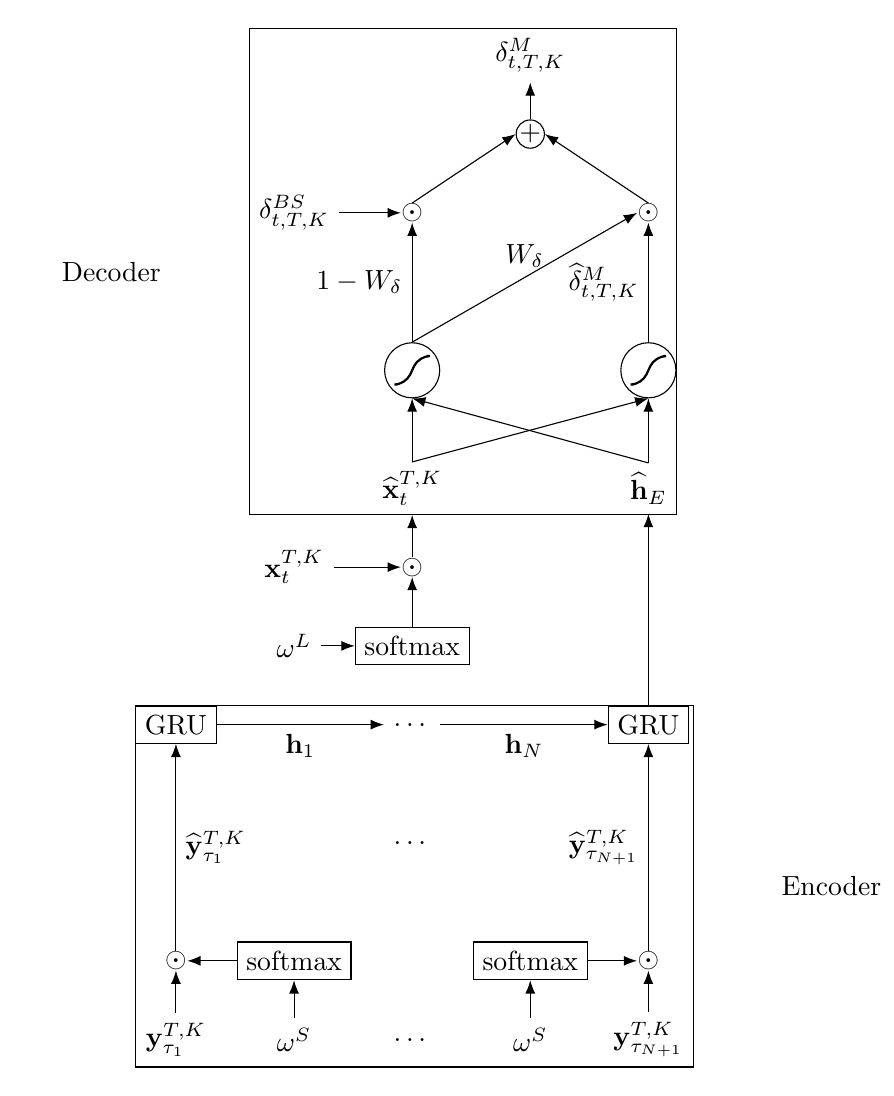
\begin{tikzpicture}[
		prod/.style={circle, draw, inner sep=0pt},
		ct/.style={circle, draw, inner sep=5pt, ultra thick, minimum width=10mm},
		ft/.style={circle, draw, minimum width=8mm, inner sep=1pt},
		filter/.style={circle, draw, minimum width=7mm, inner sep=1pt, path picture={\draw[thick, rounded corners] (path picture bounding box.center)--++(65:2mm)--++(0:1mm);
				\draw[thick, rounded corners] (path picture bounding box.center)--++(245:2mm)--++(180:1mm);}},
		mylabel/.style={font=\scriptsize\sffamily},
		>=LaTeX
		]
		
		
		\node[draw,rectangle]  (s1) at (4.5, -3) {softmax};
		\node[draw,rectangle]  (s3) at (7.5, -3) {softmax};
		\node [inner sep=0pt] (rp1) at (3*1, -3) {$\odot$};
		\node  (rp2) at (3*2, -1.5) {$\dots$};
		\node [inner sep=0pt] (rp3) at (3*3, -3) {$\odot$};
		
		\foreach \i [count=\step from 1] in {$\vy^{T,K}_{\tau_{1}}$,$\dots$,$\vy^{T,K}_{\tau_{N+1}}$}
		\node (ri\step) at (3*\step, -4) {\i};
		\node  (sw1) at (4.5, -4) {$\omega^S$ };
		\node  (sw3) at (7.5, -4) {$\omega^S$};
		\draw[->] (s1.west) to node[below]{} (rp1.east);
		\draw[->] (s3.east) to node[below]{} (rp3.west);
		\draw[->] (ri1.north) to (rp1.south);
		\draw[->] (ri3.north) to (rp3.south);
		\draw[->] (sw1.north) to (s1.south);
		\draw[->] (sw3.north) to (s3.south);
		\node (h2) at (3*2, 0.0) {$\dots$};
		\foreach \step in {1,3} {
			\node[draw,rectangle] (h\step) at (3*\step, 0.0) {GRU};
		}
		\draw[->] (rp1.north) to node[right]{$\widehat{\vy}^{T,K}_{\tau_{1}}$} (h1.south);
		\draw[->] (rp3.north) to node[left]{$\widehat{\vy}^{T,K}_{\tau_{N+1}}$} (h3.south);
		
		%\draw[->] (i4) -> (h4.south);
		\draw[->] (h1.east) to node[below]{$\vh_1$} (h2.west);
		\draw[->] (h2.east) to node[below]{$\vh_{N}$} (h3.west);
		%\foreach \step in {1,...,2} {
		%	\pgfmathtruncatemacro{\next}{add(\step,1)}
		%	\draw[->] (h\step.east) -> (h\next.west);
		%}
		\node[fit=(ri1) (ri3) (s1) (s3) (h1) (h3), draw, inner sep=0pt] (fit1) { };
		\node[align=center, outer sep=0] (encoder) [right=of fit1] {Encoder};
		
		
		
		\node[filter] (oe2) at (9, 4.5) {};
		\node[filter] (oe3) at (6, 4.5) {};
		\node [inner sep=0pt] (oe4) at (6, 6.5) {$\odot$};
		\node [inner sep=0pt] (oe5) at (9, 6.5) {$\odot$};
		\node [draw,circle,inner sep=0pt] (oe6) at (7.5, 7.5) {$+$};
		\node (oe7) at (7.5, 8.5) {$\delta^M_{t,T,K}$};
		\node  (bs) at (4.5, 6.5) {$\delta^{BS}_{t,T,K}$};
		\draw[->] (oe3.north) to node[left]{$1-W_{\delta} $} (oe4.south);
		\draw[->] (oe3.north) to node[above]{$W_{\delta}$} (oe5.west);
		\draw[->] (oe2.north) to node[left]{$\widehat{\delta}^M_{t,T,K}$} (oe5.south);
		\draw[->] (oe4.north) to node[left]{} (oe6.west);
		\draw[->] (oe5.north) to node[left]{} (oe6.east);
		\draw[->] (oe6.north) to node[left]{} (oe7.south);
		\draw[->] (bs.east) to node[left]{} (oe4.west);
		
		
		
		
		\node[inner sep=0pt]  (l1) at (6, 2) {$\odot$};
		\node[draw,rectangle]  (l3) at (6, 1) {softmax};
		\node  (l2) at (4.5, 2) {$\vx^{T,K}_{t}$};
		\node  (l4) at (4.5, 1) {$\omega^L$};
		\draw[->] (l4.east) to (l3.west);
		\draw[->] (l2.east) to (l1.west);
		\draw[->] (l3.north) to node[left]{} (l1.south);
		
		
		\node (he2) at (6, 3) {$\widehat{\vx}^{T,K}_{t}$};
		\node (he3) at (9, 3) {$\widehat{\mathbf{h}}_E$};
		\draw[->] (l1.north) to (he2.south);
		\draw[->] (h3.north) to  (he3.south);
		\draw[->] (he3.north) to  (oe2.south);
		\draw[->] (he3.north) to  (oe3.south);
		
		\draw[->] (he2.north) to (oe2.south);
		\draw[->] (he2.north) to (oe3.south);
		
		\node[fit=(oe2) (oe3) (oe5) (oe6)  (oe7)  (bs) (he2) (he3), draw, inner sep=0pt] (fit3) { };
		\node[align=center, outer sep=0] (encoder) [left=of fit3] {Decoder};
		\end{tikzpicture}
	}
	\caption{ $\model$: GRU encode-decoder hedging model. 
		The encoder summarizes the time series $\mathbf{Y}_{t}^{T,K}=\left[\vy^{T,K}_{\tau_{1}},\dots,\vy^{T,K}_{\tau_{N+1}}\right]$ as a succinct  vector $\widehat{\mathbf{h}}_E$. The decoder outputs the hedging position based on the vector $\widehat{\mathbf{h}}_E$ and the local feature vector $\vx^{T,K}_{t}$ observed at the hedging time $t$. More specifically, in the decoder, a candidate output $\widehat{\delta}^M_{t,T,K}$ is firstly produced. The final output $\delta^M_{t,T,K}$ is computed based on the linear combination of BS delta $\delta^{BS}_{t,T,K}$ and the candidate output  $\widehat{\delta}^M_{t,T,K}$. The combination weight is determined by  $W_{\delta}$. The feature weight $\omega^L$ and $\omega^S$ are used to produce the weighted local feature and  $\widehat{\vx}^{T,K}_{t}$ and weighted sequential feature $\widehat{\vy}^{T,K}_{\tau}$ respectively. The weighting acts as a feature selection process.
		Each edge in the graph has an arrow on it, pointing from a node whose output is used by the node pointed by the arrow as an input.  }
	\label{fig:RNNModel}
\end{figure}

\subsection{Feature Selection via Embedded Feature Weighting}
 Feature selection improves machine learning performance by eliminating noise and providing better interpretability. While various feature selection frameworks have  been proposed,  we consider the feature weighting method \citep{tayal2014primal}, which embeds feature selection  in the SVM training.
  This  embedded feature weighting method is shown to outperform other state-of-the-art embedded feature selection methods \citep{tayal2014primal}.
We adopt a similar feature weighting embedding technique in the discrete GRU model to conduct feature selections on both the local feature $\vx^{T,K}_{t}$ and the sequential feature $\mathbf{Y}_{t}^{T,K}$.
Features are first weighted and then fed into the encoder and decoder as inputs. Feature weights are optimized during model training.

We  use a softmax function to generate a normalized  feature weighting vector. For the local feature $\vx^{T,K}_{t}  \in \Real^{d_l}$, the $j^\text{th}$ component of the normalized weight vector is given by
\[
\frac{exp(\omega^L_j)}{\sum_{i=1}^{d_l} exp(\omega^L_i)}
\]
The weighted  local feature vector is defined as
\[\widehat{\vx}^{T,K}_{t}=\frac{exp(\omega^L)}{\sum_{i=1}^{d_l} exp(\omega^L_i)}\odot \vx^{T,K}_{t} \] 
where $\odot$ denotes the element-wise multiplication.

Similarly,
for the sequential feature $\mathbf{y}_{\tau_i}^{T,K}$,  the $j^\text{th}$ component of the normalized weight vector is given by
\[
\frac{exp(\omega^S_j)}{\sum_{i=1}^{d_s} exp(\omega^S_i)}
\]
%The normalized weight vector for sequential feature is therefore \[\mathbf{\zeta}=[\zeta_1,\dots,\zeta_{d_s}]\]
% Recall that $\mathbf{y}_{\tau_i}^{T,K}$ is a vector of the ${d_s}$ features.
  The weighted feature vector at time  $\tau_i$ is defined as
\[
\widehat{\vy}_{\tau_i}^{T,K} =\frac{exp(\omega^S)}{\sum_{j=1}^{d_s} exp(\omega^S_j)} \odot \mathbf{y}_{\tau_i}^{T,K}
\]
{The weighting procedure acts as a feature selection.}
If a  particular feature is not relevant in predicting the hedging position, the associated weight after learning  is expected to be negligible.
%The unnormalized feature weight vectors $LW$ and $SW$ are parts of the parameters to be learned for the model. The model will be trained to adjust the weight dynamically.


\subsection{GRU Encoder}
The  proposed $\model$  in Figure \ref{fig:RNNModel} has an one-layer GRU, which encodes the sequential feature $\mathbf{Y}_{t}^{T,K}$ to  a fixed-sized vector
$\mathbf{\widehat{h}}_E$ .
At the  step $i$,  the encoder computes the value of the hidden state $\vh_{i}$ using a GRU cell. The input at the step $i$ of the encoder is $\widehat{\vy}^{T,K}_{\tau_{i}}$,  $i=1,\ldots,N+1$.
The internal structure of the GRU cell is shown in Figure \ref{fig:RNN}.

Let  $\vW_z,\vU_z,\vb_z,\vW_r,\vU_r, \vb_r,\vW_h,\vU_h,\vb_h$  denote
parameters shared by all GRU cells.


\begin{enumerate}
	\item The \textbf{update gate} decides how much the cell updates its activation:
	\[\mathbf{z}_i= sigmoid ( \vW_z \widehat{\vy}^{T,K}_{\tau_{i}} + \vU_z \vh_{i-1} +\vb_z)\]
	\item The \textbf{reset gate} decides how much  information to retain from the  previous hidden state $\vh_{i-1}$:
	\[\mathbf{r}_i= sigmoid ( \vW_r \widehat{\vy}^{T,K}_{\tau_{i}} + \vU_r \vh_{i-1} +\vb_r)\]
	\item The \textbf{candidate} hidden state value $\widehat{\vh}_i$ is computed from the current input $\widehat{\vy}^{T,K}_{\tau_{i}}$,  previous hidden state $\vh_{i-1}$, and the reset value $\mathbf{r_i}$ :
	\[
	\widehat{\vh}_i=tanh( \vW_h \widehat{\vy}^{T,K}_{\tau_{i}}  + \vU_h (\mathbf{r}_i \odot \vh_{i-1}) +\vb_h)
	\]
	\item  The \textbf{output} hidden state value $\vh_{i}$ is  computed based on a weighted combination of the previous activation $\vh_{i-1}$ and the candidate activation $\widehat{\vh}_i$:
	\[
	\vh_i=(1-\mathbf{z}_i) \odot \vh_{i-1} + \mathbf{z}_i \odot \widehat{\vh}_i
	\]
\end{enumerate}







\begin{figure}[htp!]
	\centering
			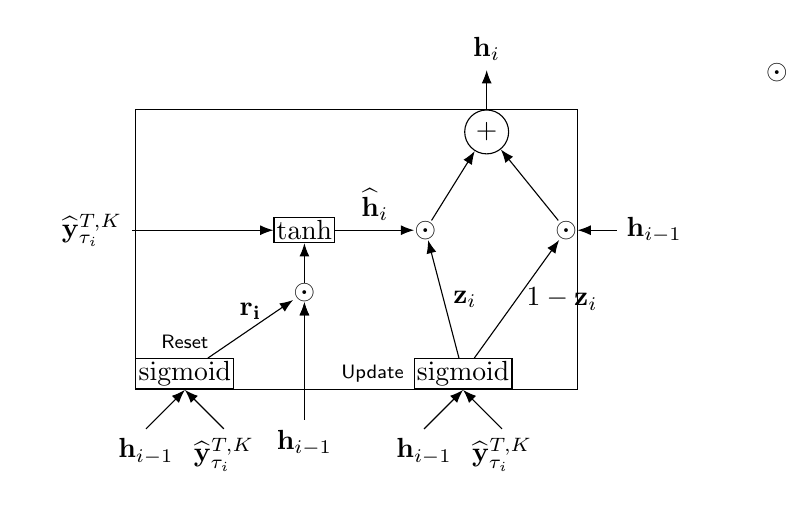
\begin{tikzpicture}[
			prod/.style={circle, draw, inner sep=0pt},
			ct/.style={circle, draw, inner sep=5pt, ultra thick, minimum width=10mm},
			ft/.style={circle, draw, minimum width=8mm, inner sep=1pt},
			filter/.style={circle, draw, minimum width=7mm, inner sep=1pt, path picture={\draw[thick, rounded corners] (path picture bounding box.center)--++(65:2mm)--++(0:1mm);
					\draw[thick, rounded corners] (path picture bounding box.center)--++(245:2mm)--++(180:1mm);}},
			mylabel/.style={font=\scriptsize\sffamily},
			>=LaTeX
			]
			\node[draw, rectangle,inner sep=1pt] (ct) {tanh};
			\node[inner sep=0pt]  (l1) at (6, 2) {$\odot$};
			\node[ right=10mm of ct,inner sep=0pt] (int1) {$\odot$};
			\node[ right=15mm of int1,inner sep=0pt] (x1) {$\odot$};
			\node[left=of ct] (x2) {};
			\node[ below=5mm of ct,inner sep=0pt] (x3) {$\odot$};
			\node[draw, rectangle,inner sep=1pt, below=15mm of x2, label={[mylabel]above:Reset}] (ft) {sigmoid};
			\node[draw, rectangle,inner sep=1pt, right=22.75mm of ft, label={[mylabel]left:Update}] (ot) {sigmoid};
			
			\node[above=of x1] (temp) {};
			\node[prod, left= 6mm of temp,inner sep=2pt] (final) {$+$};
			\draw[->] (ft) to  node[above]{$\mathbf{r_i}$} (x3);
			\draw[->] (ot) to  node[right]{$1-\mathbf{z}_i$} (x1);
			\draw[->] (ot) to  node[right]{$\mathbf{z}_i$} (int1);
			\draw[->] (ct) to  node[above]{$\widehat{\vh}_i$} (int1);
			
			\draw[->] (x3) to  (ct);
			\draw[->] (x1) to  (final);
			\draw[->] (int1) to  (final);
			\node[fit= (ot) (ft) (x1) (x3) (final), draw, inner sep=0pt] (fit) {};
			\draw[->] (fit.south-|ct) to (x3);
			
			
			
			
			
			\draw[<-] (fit.south-|ot) coordinate (aux)--++(-45:7mm) node[below]{$\widehat{\vy}^{T,K}_{\tau_{i}}$ };
			\draw[<-] (fit.south-|ot) coordinate (aux)--++(-135:7mm) node[below]{$\vh_{i-1}$};
			
			\draw[<-] (fit.south-|ft) coordinate (aux)--++(-135:7mm) node[below]{ $\vh_{i-1}$};
			\draw[<-] (fit.south-|ft) coordinate (aux)--++(-45:7mm) node[below]{$\widehat{\vy}^{T,K}_{\tau_{i}}$ };
			
			\draw[<-] (x3.south) coordinate (aux)--++(-90:15mm) node[below]{$\vh_{i-1}$ };
			\draw[<-] (ct.west) coordinate (aux)--++(180:18mm) node[left]{$\widehat{\vy}^{T,K}_{\tau_{i}}$ };
			
			\draw[<-] (x1.east) coordinate (aux)--++(0:5mm) node[right]{$\vh_{i-1}$ };
			\draw[->] (final.north) coordinate (aux)--++(90:5mm) node[above]{$\vh_{i}$ };
			%\node[filter, below=23mm of x3, label={[mylabel]right:tanh}] (ex1) {};
			\end{tikzpicture}
	\caption{Illustration of the GRU cell. 
		At step $i$,  GRU cell produces a vector  $\vh_{i}$ as the current hidden states based on the hidden states produced from the previous steps $\vh_{i-1}$  and the input $\widehat{\vy}^{T,K}_{\tau_{i}}$. The reset unit produces the weight $\mathbf{r}_i$ which determines how much information is retained from $\vh_{i-1}$.  
		The final output from the GRU cell $\vh_{i}$ is  computed based on a weighted combination of the previous activation $\vh_{i-1}$ and the candidate activation $\widehat{\vh}_i$, where the combination weight $\mathbf{z}_i$ is produced by the update unit. Each edge in the graph has an arrow on it, pointing from a node whose output is used by the node pointed by the arrow as an input.}
	\label{fig:RNN}
\end{figure}
The hidden state at the last step $\vh_{N+1}$, corresponding to time ${\tau_{N+1}}={t}$, is supplied to
the decoder as the fixed size vector $\mathbf{\widehat{h}}_E$, which  extracts relevant information in $\mathbf{Y}_{t}^{T,K}$.
\subsection{Decoder}

The decoder combines the output of the encoder from the sequential feature $\mathbf{Y}_{t}^{T,K}$  at the hedging time $t$ with the current local feature $\mathbf{x}_{t}^{T,K}$.
It uses one neural network to first compute a candidate output  $\widehat{\delta}^M_{t,T,K}$,  based on both the weighted local input  $\widehat{\vx}_{t}^{T,K}$ and the fixed size vector $\mathbf{\widehat{h}}_E$ :
$$
\widehat{\delta}^M_{t,T,K}=sigmoid (\vv^T_{out} \ tanh( \vU_{out} \mathbf{\widehat{h}}_E + \vW_{out} \widehat{\vx}_{t}^{T,K}+ \vb_{out})).
$$

The the output gate value $W_{\delta}$ is given by another neural network, based on both the weighted local input  $\widehat{\vx}_{t}^{T,K}$ and the fixed size vector $\mathbf{\widehat{h}}_E$ :
\begin{equation}\label{WDel}
W_{\delta}=sigmoid (\vv^T_{Gate} \ tanh( \vU_{Gate} \mathbf{\widehat{h}}_E + \vW_{Gate} \widehat{\vx}_{t}^{T,K}+ \vb_{Gate})).
\end{equation}

The practitioner's BS delta encapsulates a significant portion of the sensitivity of the option price to the underlying and has been adopted in option hedging practice. Therefore we use BS implied volatility delta as a pre-trained model in the designed $\model$ to utilize both local and sequential features to minimize hedge risk.
Specifically, the output of the proposed  $\model$ is a linear combination of the candidate output $\widehat{\delta}^M_{t,T,K}$ and the BS delta $\delta^{BS}_{t,T,K}$ computed from the implied volatility at the hedging time $t$ for the option with expiry $T$ and strike $K$. In addition,  different combination formulae are used when training for different types of options.
For hedging a call option, the final output from $\model$ is :
\begin{equation}
\delta^M_{t,T,K}=\widehat{\delta}^M_{t,T,K} \times W_{\delta} +\delta^{BS}_{t,T,K} \times (1-W_{\delta})
\label{eq:call}
\end{equation}
For hedging a put option, the final output from the model is:
\begin{equation}
\delta^M_{t,T,K}=-\widehat{\delta}^M_{t,T,K} \times W_{\delta} +\delta^{BS}_{t,T,K} \times (1-W_{\delta})
\label{eq:put}
\end{equation}
where $\widehat{\delta}^M_{t,T,K}$ is the candidate output.
When $W_{\delta}=0$,  $\delta^{BS}_{t,T,K}$  is the output and, when $W_{\delta}=1$,  the output  is the candidate $\widehat{\delta}^M_{t,T,K}$. The combination weight $W_{\delta}$
%, for $\widehat{\delta}^M_{t,T,K}$ and $\delta^{BS}_{t,T,K}$ respectively,
is defined in \eqref{WDel}.
  The sigmoid function is used as the final activation function because, under the Black-Scholes-Merton framework \citep{black1973pricing}, the range of the hedging position for call options is $[0,1]$ and  the range of the hedging position for put options is $[-1,0]$. It can be easily shown that $\delta^M_{t,T,K}$, given by \eqref{eq:call}, is within $[0,1]$ and  $\delta^M_{t,T,K}$, given by \eqref{eq:put}, is within $[-1,0]$.

\subsection{Robust Loss Function}

At the hedging time $t_i$, for the data instance $i$ with  strike $K_i$, and expiry $T_i$ , the local discrete hedging loss is:
\[
loss_i=\Delta V^{mkt}_{t_i,T_i,K_i}-\DS_{t_i} \delta^M_{{t_i,T_i,K_i}}
\]
where  $\delta^M_{{t_i,T_i,K_i}}$ is the corresponding  final output from $\model$,  $\DS_{t_i}$ denotes the change in the market underlying price, and $\Delta V^{mkt}_{t_i,T_i,K_i}$ denotes the change in the market option price,  see \eqref{eq:DVDS}.
Let $M$ be the number of data instances.
The objective function used in the data-driven regularized kernel hedging model  in \citep{knian2017} is the mean squared loss,
\begin{equation}
MSE=\frac{1}{2M} \sum_{i=1}^{M} loss_i^2.
\label{l1}
\end{equation}
Since the quadratic error function is sensitive to outliers, in this work,
we additionally incorporate the Huber loss function  \citep{Huber1964robust}  below in the proposed $\model$:
\[
HE=\frac{1}{M} \sum_{i=1}^{M} Huber(loss_i),
\]
where $Huber(\cdot)$ is as defined below:
\[
Huber(loss,\mathcal{T})=\left\{ \begin{array}{ll }
\frac{1}{2} loss^2  , \;&  \text{if} \; |loss|\leq \mathcal{T}\\
\mathcal{T}(|loss|-\frac{1}{2}\mathcal{T}), \; &\text{otherwise}
\end{array} \right.
\]
The Huber loss \citep{Huber1964robust} has been shown to be more robust than the squared loss with respect to toutliers, when  the threshold parameter $\mathcal{T}$ is carefully chosen {\em a priori}.
In the context of machine learning, the parameter $\mathcal{T}$ can be tuned but this can be computationally expensive. In the proposed
$\model$, since delta from the BS model  with the implied volatility   is used as a pre-trained model, we adaptively set the thresholding parameter $\mathcal{T}$ to be absolute value of the hedging error from the Black–Scholes delta of the data instance $i$, i.e.,
\begin{equation}\label{eq:thresh}
\mathcal{T}_i=|\Delta V^{mkt}_{t_i,T_i,K_i}-\DS_{t_i} \delta^{BS}_{t_i,T_i,K_i}|
\end{equation}
where $\delta^{BS}_{t_i,T_i,K_i}$ is the Black–Scholes delta using implied volatility for data instance $i$.
The modified Huber loss  becomes
\[
MHuber(loss_i,\mathcal{T}_i)=\left\{ \begin{array}{ll}
\frac{1}{2} loss_i^2  , \; &\text{if} \; |loss_i|\leq \mathcal{T}_i\\
\mathcal{T}_i(|loss_i|-\frac{1}{2}\mathcal{T}_i), \; & \text{otherwise}
\end{array} \right.
\]
Using the Huber loss with the adaptive threshholding parameter in \eqref{eq:thresh}, the objective for the proposed $\model$  is:
\begin{equation}
MHE=\frac{1}{M} \sum_{i=1}^{M} MHuber(loss_i,\mathcal{T}_i)
\label{l2}
\end{equation}







\section{Training $\model$} \label{sec:train}
Next we discuss training  $\model$,  including initialization,  pre-training,  optimization, and regularization.
\subsection{Initialization}\label{sec:init}
When training a RNN model,  an initial weight matrix is typically chosen as a random orthogonal matrix. Since the orthogonal initialization  can often speed up training \citep{le2015simple}, all the weight matrices   are initialized as orthogonal random matrices in training $\model$. The random orthogonal matrices are   Householder transformations of random matrices \citep{le2015simple}.

\subsection{Optimization}
First-order optimization methods, such as stochastic gradient descent (SGD) and its extensions,  are the most widely used optimization methods in machine learning, due to  their low computational costs. Despite their wide usage,  well-known deficiencies when  training highly non-convex objective functions, including  relatively-slow convergence, sensitivity to hyper-parameter values (e.g., learning rate), stagnation at high training errors, and difficulty in escaping flat regions and saddle points \citep{yao2018inexact}.

More recently,  improved SGD methods such as ADAM \citep{kingma2014adam}, have been proposed.
These methods seem to achieve significantly better solutions compared with earlier SGD. However,  it has recently been empirically observed in \cite{reddi2019convergence}  that these algorithms sometimes fail to converge to a first-order critical point due to the exponential moving average used in the algorithms.
%These algorithms are based on using gradient updates scaled by square roots of exponential moving averages of squared past gradients and


Since the data size and the number of the parameters in $\model$ are relatively small (which is a distinguishing characteristics of many financial data mining  problems), it is computationally feasible to apply a second order optimization method.  Furthermore, the recently proposed trust-region sub-problem solver \citep{lenders2018trlib} computes the trust region sub-problem solution iteratively requiring only Hessian-vector products. % avoiding direct computation of the Hessian matrix and  Hessian matrix factorizations.
Consequently we use a trust region method, which is shown in Algorithm \ref{alg:trust} when training $\model$.  The meta-parameters for trust-region algorithm are shown in Table \ref{para2}. 
\begin{table}[htp!]
	\begin{center}
	\begin{tabular}{|c|c|c|c|c|c|c|}
	\hline
	$\mathcal{R}_0$&
	$\epsilon_{\theta}$& 
	$\epsilon_{r}$&
	$\eta_{r_1}$&
	$\eta_{r_2}$&
	$\gamma_u$&
	$\gamma_d$  \\ \hline
	 1.0&$10^{-5}$&$10^{-8}$&0.25&0.75 &2 & 0.5  \\    \hline
	\end{tabular}
	\end{center}
	
	\caption{Meta-parameters for the trust-region algorithm. The trust-region algorithm is used for training  all the data-driven models based on neural network framework in this thesis.}
	\label{para2}
	\end{table}



 \begin{algorithm}[htp!]
	%\DontPrintSemicolon
	\SetAlgoNoLine
	
	\KwIn{$\theta_0 \in \Real^n$: initial vector of parameters.\newline
		$Obj(\theta)$: the objective function (For $\model$, we use either \eqref{l1} or  \eqref{l2}. For $\modelT$, we use \eqref{eq:totalObjLinear}. For  $\modelL$, we use \eqref{eq:totalObjLinear}.  )\newline
		$\mathcal{R}_0$: initial trust region radius \newline
		$\epsilon_{\theta}$: tolerance for the norm of the gradient \newline
		$\epsilon_{r}$: tolerance for the trust region radius \newline
		$\eta_{r_1}$: first threshold  for update the trust region radius \newline
		$\eta_{r_2}$: second threshold  for update the trust region radius \newline
		$\gamma_u>1$: ratio to increase the trust-region radius \newline
		$\gamma_d<1$: ratio to decrease the trust-region radius}
	\KwOut{
		$\theta^*$: the vector of parameters that minimize the objective function $Obj(\theta)$
	}
	
	\Begin{
		$k=0$\;
		\While{$\|\nabla Obj(\theta_k)\|_2 \geq \epsilon_{\theta} $ \text{and} $\mathcal{R}_k \geq \epsilon_r$  }{
			solve the trust-region subproblem \cite{lenders2018trlib}:
			\[
			\begin{split}
			s^*_k=\argmin_s\;& m_k(s)=Obj(\theta_k)+s^T \nabla Obj(\theta_k)+ s^T \nabla^2 Obj(\theta_k) s \\
			\text{sub to}& \|s\|_2 \leq \mathcal{R}_k
			\end{split}
			\]
			define
			\[
			\mathcal{P}_k=\frac{Obj(\theta_k)-Obj(\theta_k+s^*_k)}{Obj(\theta_k)-m_k(s^*_k)}
			\]
			Update the radius:
			\eIf{$\eta_{r_2}>\mathcal{P}_k < \eta_{r_1}$}
			{$\theta_{k+1}=\theta{k}+s^*_k$}
			{$\theta_{k+1}=\theta{k}$}
			\[
				\mathcal{R}_{k+1}=\left\{ 
				\begin{array}{ll}
					\gamma_u  \|s^{*}_k\|_2
					  , \; &\text{if} \; \mathcal{P}_k < \eta_{r_1}\\


					   \mathcal{R}_k
					  , \; &\text{if} \; \eta_{r_1} \leq \mathcal{P}_k \leq \eta_{r_2}\\

					 \max(\gamma_u \|s^{*}_k\|_2,\mathcal{R}_k)
					  , \; &\text{if} \; \mathcal{P}_k >\eta_{r_2}
				\end{array} \right.
    		 \]
			k=k+1
		}
		\[
		\theta^*=\theta_k
		\]
		
		
		
		
		
	}
	\SetAlCapSkip{5em}
	\IncMargin{1em}
	\caption{Trust-region Algorithm}  \label{algorithm}
	\label{alg:trust}
	\DecMargin{1em}
\end{algorithm}




\subsection{Pre-training and  Regularization} \label{sec:preT}
We use  early stopping as the regularization \citep{raskutti2014early}.
 %We evaluate hedging performance using the gain ratio defined in \citep{hulloptimal}, which is the average quadratic hedging error of a hedging method over the average quadratic hedging error of the implied volatility BS delta hedging. The average quadratic hedging error is equal to the variance when the mean of the hedging error is zero.
At each training date, we reserve a fraction of the observed data to be the validation set. The rest of the observed data is used as the training set. The performance on the validation set is used to determine when over-fitting begins. Let $\theta$ denote the set of parameters to be learned for the proposed $\model$. After each training step $k$,  the model performance is evaluated on the validation set and the associated parameters $\theta_k$ is recorded.  Model training optimization is performed on the training set until the trust-region optimizer terminates. The parameters that achieve the best performance on the validation set  is used to predict the hedging position for the testing data instances.

For $\model$,  the training optimization problem  is nonconvex,   which can benefit from a good initial model.   We choose the initial model for the training  problem  by matching  the output of $\model$ to  the pre-trained BS model  $\delta^{BS}_{t,T,K}$.  Specifically,  we determine the initial model for training optimization by solving the nonlinear least square problem below,
\begin{equation}\label{NLS}
\min \frac{1}{2M} \sum_{i=1}^{M} ( \delta^M_{t_i,T_i,K_i} -\delta^{BS}_{t_i,T_i,K_i})^2,
\end{equation}
where the starting point for \eqref{NLS} is a set of randomly initialized  weight matrices, as described in section \ref{sec:init}.

Using a solution to \eqref{NLS} as the initial model, we train $\model$ with the robust objective function \eqref{l2}. Recall that the  output of  $\model$, either \eqref{eq:call} or \eqref{eq:put}, is a linear combination of the candidate output $\widehat{\delta}^M_{t,T,K}$ and the BS delta $\delta^{BS}_{t,T,K}$ computed from the implied volatility. When $W_{\delta}$ approaches 0, the  output of  $\model$ converges to $\delta^{BS}_{t,T,K}$ as the output. When  $W_{\delta}$ approaches $1$,   $\model$ outputs  candidate $\widehat{\delta}^M_{t,T,K}$.
This simple combination structure allows the pre-training phase to be finished in just a few training steps.\footnote{Note that we will also stop the pre-training when $W_{\delta}>0.97.5$ or $W_{\delta}<0.025$. This is because, when we have $W_{\delta}>0.97.5$ or $W_{\delta}<0.025$, due to saturating gradient problem of the sigmoid function, the initial gradient, when training with actual local hedging objective,  will be very small. This will slow down the first few  learning steps when training with actual local hedging objective.}
The pre-training stage guarantees that the initial performance of the model on the validation set is close to $\delta^{BS}_{t,T,K}$. If the output from the model after training performs worse than $\delta^{BS}_{t,T,K}$ on the validation set, we use the initial model after pre-training.


Additionally  the validation set is also used to select  whether to use the mean square objective function \eqref{l1} or  the modified Huber loss objective \eqref{l2} . The model trained with the objective function that performs better on the validation set is used when predicting the hedging position of the testing data instances, which are unobserved at the time of training.


\subsection{Model Re-use and  Re-initialization}\label{sec:reuse}
In contrast to the regularized kernel method in \citep{knian2017},  one advantage of the proposed $\model$ is
that the parameters from one trained model can be readily reused as the starting point for the model training on a subsequent rebalancing day.
This allows a model to be updated more frequently, adapting to market changes without completely rebuilding a model.
The kernel method in \citep{knian2017}, on the other hand,  recomputes the kernel matrix at each rebalancing time, which requires $O(m^3)$ computation assuming a completely new kernel matrix. Thus, updating the model frequently using the kernel method in \citep{knian2017} is computationally prohibitive.



An artificial neural network is known to potentially suffer catastrophic interference or catastrophic forgetting \citep{mccloskey1989catastrophic}, i.e., a model  forgets completely and abruptly previously learned information upon observing new information.
When this happens, the resulting broken model usually has poor generalization ability. If a broken model with poor generalization ability is allowed to be continually updated,  the performance of all the future models may be negatively affected. Thus, whenever a worse performance, in comparison to   $\delta^{BS}_{t,T,K}$ , is observed on a validation set,  we re-initialize the parameters of  $\model$ and pre-train the model again. This avoids continually updating the broken model.  %Model re-initialization can happen frequently when a market change frequently.
If after model re-initialization and training, the performance of the proposed $\model$ remains worse than that of  $\delta^{BS}_{t,T,K}$ on the validation set, we simply output $\delta^{BS}_{t,T,K}$.
%to avoid a potential poor performance on the testing data. % due to adoption of the early stopping regularization.

In summary, we initialize the model as described in section \ref{sec:init} and \ref{sec:preT} on the first testing date. When we train the model,  %on other testing dates, 
we reuse the parameters from the previously trained model as the starting point unless the performance of the proposed $\model$ is worse than that of $\delta^{BS}_{t,T,K}$,
%When the performance of the proposed $\model$ is worse than that of  $\delta^{BS}_{t,T,K}$, 
in which case we re-initialize the parameters of the proposed $\model$ and train the model again.
\section{Alternative Data-Driven Hedging Models Under Neural Network Framework}
\label{sec:alternativeModel}
Lastly, before jumping into the real data experimental results for local discrete hedging in Chapter \ref{sec:LocalComparison}, we introduce the following supplementary models:
\begin{enumerate}
	\item To gain insights on the roles of the decoder and encoder in the proposed $\model$,  we  also consider a decoder only model $\modelN$, which corresponds to removing the encoder from $\model$ in Figure \ref{fig:DNN}.  We train  $\modelN$ in the same way  as described in section \ref{sec:train}. 
	\item To gain insights on the role of output gate and robust Huber loss, we remove the output gate part of the decoder model. The resulting model  is shown in Figure \ref{fig:DRNNC}. In other words, the output $\delta^M$ is purely based $\mathbf{\widehat{h}}_E$ and $ \widehat{\vx}_{t}^{T,K}$:
	\[
		{\delta}^M_{t,T,K}=sigmoid (\vv^T_{out} \ tanh( \vU_{out} \mathbf{\widehat{h}}_E + \vW_{out} \widehat{\vx}_{t}^{T,K}+ \vb_{out})).
	\]
	We denote the model shown in Figure \ref{fig:DRNNC} as $\textsc{GRU}_{c}$. The training procedure of $\textsc{GRU}_{c}$ is slightly different from $\model$:
	\begin{itemize}
		\item The objective function is fixed to be the mean squared loss.
	\end{itemize}
\end{enumerate}

\begin{figure}
	\centering
	\resizebox{0.40\textwidth}{!}{
		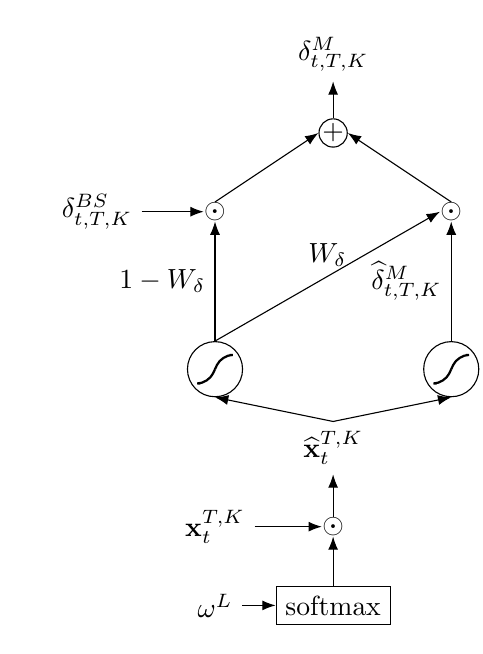
\begin{tikzpicture}[
		prod/.style={circle, draw, inner sep=0pt},
		ct/.style={circle, draw, inner sep=5pt, ultra thick, minimum width=10mm},
		ft/.style={circle, draw, minimum width=8mm, inner sep=1pt},
		filter/.style={circle, draw, minimum width=7mm, inner sep=1pt, path picture={\draw[thick, rounded corners] (path picture bounding box.center)--++(65:2mm)--++(0:1mm);
				\draw[thick, rounded corners] (path picture bounding box.center)--++(245:2mm)--++(180:1mm);}},
		mylabel/.style={font=\scriptsize\sffamily},
		>=LaTeX
		]
		\node[filter] (oe2) at (9, 5) {};
		\node[filter] (oe3) at (6, 5) {};
		\node [inner sep=0pt] (oe4) at (6, 7) {$\odot$};
		\node [inner sep=0pt] (oe5) at (9, 7) {$\odot$};
		\node [draw,circle,inner sep=0pt] (oe6) at (7.5, 8) {$+$};
		\node (oe7) at (7.5, 9) {$\delta^M_{t,T,K}$};
		\node  (bs) at (4.5, 7) {$\delta^{BS}_{t,T,K}$};
		\draw[->] (oe3.north) to node[left]{$1-W_{\delta}$} (oe4.south);
		\draw[->] (oe3.north) to node[above]{$W_{\delta}$} (oe5.west);
		\draw[->] (oe2.north) to node[left]{$\widehat{\delta}^M_{t,T,K}$} (oe5.south);
		\draw[->] (oe4.north) to node[left]{} (oe6.west);
		\draw[->] (oe5.north) to node[left]{} (oe6.east);
		\draw[->] (oe6.north) to node[left]{} (oe7.south);
		\draw[->] (bs.east) to node[left]{} (oe4.west);
		\node (he2) at (7.5, 4) {$\widehat{\vx}_{t}^{T,K}$};
		\draw[->] (he2.north) to (oe2.south);
		\draw[->] (he2.north) to (oe3.south);
		
		\node[inner sep=0pt]  (l1) at (7.5, 3) {$\odot$};
		\node[draw,rectangle]  (l3) at (7.5, 2) {softmax};
		\node  (l2) at (6, 3) {$\vx_{t}^{T,K}$};
		\node  (l4) at (6, 2) {$\omega^L$};
		\draw[->] (l4.east) to (l3.west);
		\draw[->] (l2.east) to (l1.west);
		\draw[->] (l3.north) to  (l1.south);
		\draw[->] (l1.north) to (he2.south);
		
		
		\end{tikzpicture}
	}\caption{$\modelN$: decoder GRU only. 
	This simplified model only retains the decoder. The decoder computes the hedging position solely based on the information vector $\vx_{t}^{T,K}$ observed at time $t$. A candidate output $\widehat{\delta}^M_{t,T,K}$ is produced. The final output $\delta^M_{t,T,K}$ is computed based on the linear combination of BS delta $\delta^{BS}_{t,T,K}$ and the candidate output  $\widehat{\delta}^M_{t,T,K}$. The combination weight is determined by  $W_{\delta}$. The feature weight $\omega^L$ is used to produce the weighted local feature   $\widehat{\vx}^{T,K}_{t}$. The weighting acts as a feature selection process. Each edge in the graph has an arrow on it, pointing from a node whose output is used by the node pointed by the arrow as an input.}
	\label{fig:DNN}
\end{figure}



\begin{figure}
	\centering
	\resizebox{0.80\textwidth}{!}{
			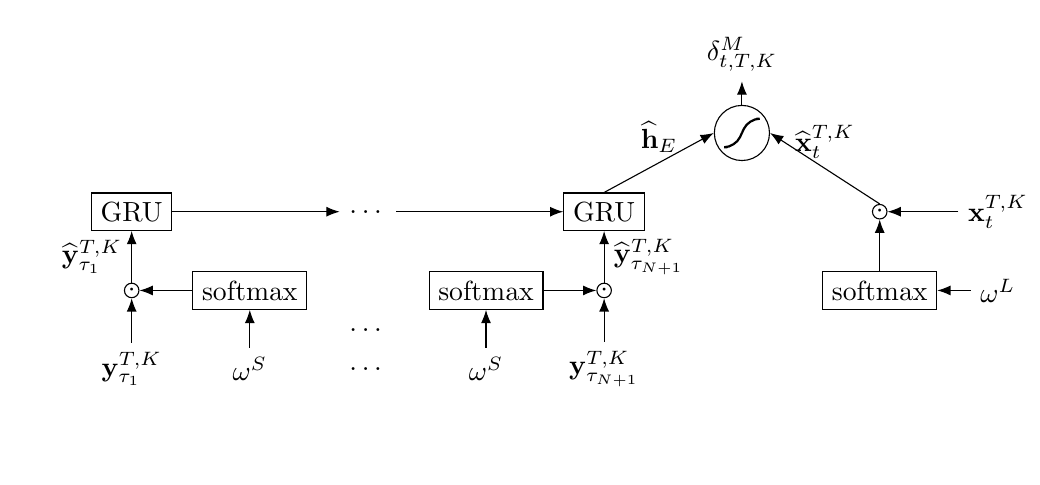
\begin{tikzpicture}[
		prod/.style={circle, draw, inner sep=0pt},
		ct/.style={circle, draw, inner sep=5pt, ultra thick, minimum width=10mm},
		ft/.style={circle, draw, minimum width=8mm, inner sep=1pt},
		filter/.style={circle, draw, minimum width=7mm, inner sep=1pt, path picture={\draw[thick, rounded corners] (path picture bounding box.center)--++(65:2mm)--++(0:1mm);
		\draw[thick, rounded corners] (path picture bounding box.center)--++(245:2mm)--++(180:1mm);}},
		mylabel/.style={font=\scriptsize\sffamily},
		>=LaTeX
		]
		
			
			\node[draw,rectangle]  (s1) at (4.5, -1) {softmax};
			\node[draw,rectangle]  (s3) at (7.5, -1) {softmax};
			\node [draw,circle,inner sep=0pt] (rp1) at (3*1, -1) {$\cdot$};
			\node  (rp2) at (3*2, -1.5) {$\dots$};
			\node [draw,circle,inner sep=0pt] (rp3) at (3*3, -1) {$\cdot$};
	
			\foreach \i [count=\step from 1] in {$\vy_{\tau_1}^{T,K}$,$\dots$,$\vy_{\tau_{N+1}}^{T,K}$}
			\node (ri\step) at (3*\step, -2) {\i};
			\node  (sw1) at (4.5, -2) {$\omega^{S}$};
			\node  (sw3) at (7.5, -2) {$\omega^{S}$};
			\draw[->] (s1.west) to  (rp1.east);
			\draw[->] (s3.east) to  (rp3.west);
			\draw[->] (ri1.north) to (rp1.south);
			\draw[->] (ri3.north) to (rp3.south);
			\draw[->] (sw1.north) to (s1.south);
			\draw[->] (sw3.north) to (s3.south);
			\node (h2) at (3*2, 0.0) {$\dots$};
			\foreach \step in {1,3} {
				\node[draw,rectangle] (h\step) at (3*\step, 0.0) {GRU};
			}
			\draw[->] (rp1.north) to node[left]{$\widehat{\vy}_{\tau_1}^{T,K}$} (h1.south);
			\draw[->] (rp3.north) to node[right]{$\widehat{\vy}_{\tau_{N+1}}^{T,K}$} (h3.south);
			
			%\draw[->] (i4) -> (h4.south);
			
			\foreach \step in {1,...,2} {
				\pgfmathtruncatemacro{\next}{add(\step,1)}
				\draw[->] (h\step.east) -> (h\next.west);
			}
		
			\node[draw,circle,inner sep=0pt]  (l1) at (12.5, 0) {$\cdot$};
			\node[draw,rectangle]  (l3) at (12.5, -1) {softmax};
			\node  (l2) at (14, 0) {$\vx_{t}^{T,K}$};
			\node  (l4) at (14, -1) {$\omega^{L}$};
			\draw[->] (l4.west) to (l3.east);
			\draw[->] (l2.west) to (l1.east);
			\draw[->] (l3.north) to  (l1.south);
	
			\node[filter] (he2) at (10.75, 1) {};
			\node (he3) at (10.75, 2) {$\delta^{M}_{t,T,K}$};
			\draw[->] (h3.north) to node[above]{$\widehat{\mathbf{h}}_E$} (he2.west);
			\draw[->] (l1.north) to node[above]{$\widehat{\vx}_{t}^{T,K}$} (he2.east);
			\draw[->] (he2.north) to (he3.south);
	
			\node at (10.75, -3) {};
			\end{tikzpicture}
	}\caption{$\textsc{GRU}_{c}$: This simplified model removes  the output gate in  the decoder. The encoder summarizes the time series $\mathbf{Y}_{t}^{T,K}=\left[\vy^{T,K}_{\tau_{1}},\dots,\vy^{T,K}_{\tau_{N+1}}\right]$ as a succinct  vector $\widehat{\mathbf{h}}_E$. The decoder outputs the hedging position based on the vector $\widehat{\mathbf{h}}_E$ and the local feature vector $\vx^{T,K}_{t}$ observed at the hedging time $t$ directly. The output gate is removed and we do not combine the output with $\delta^{BS}_{t,T,K}$ using linear combination as in Figure \ref{fig:RNNModel}.
	Each edge in the graph has an arrow on it, pointing from a node whose output is used by the node pointed by the arrow as an input.  }
	\label{fig:DRNNC}
	\end{figure}



\chapter{Local Discrete Hedging Performance Comparison Using  S\&P 500 index Options}
\label{sec:LocalComparison}
Using the S\&P 500  ({European})  index option market data from January 2, 2001 to August 31, 2015,
we  compare hedging performance of different hedging strategies.

Following \cite{hulloptimal},  we use the Gain ratio below as the evaluating measure for the hedging performance:
\[
\textsc{Gain}=1-\frac{\sum_{i=1}^m \bigg((\Delta V^{mkt}_{t_i,T_i,K_i}-\delta_{t_i,T_i,K_i} ~ \Delta S_{t_i} \bigg)^2}{\sum_{i=1}^m \bigg((\Delta V^{mkt}_{t_i,T_i,K_i}-\delta^{BS}_{t_i,T_i,K_i} ~ \Delta S_{t_i} \bigg)^2},
\]
where $m$ is the total number of data instances to be evaluated. In addition,  for the data instance $i$, corresponding to hedging option with expiry $T_i$ and strike $K_i$ at hedging time $t_i$, we recall that $\delta^{BS}_{t_i,T_i,K_i}$ is the implied Black–Scholes delta, $\delta_{t_i,T_i,K_i}$  is the hedging position from the method under consideration,  e.g., SABR delta,  MV delta,  and output from $\DKLs$ or $\model$.
  In addition $\Delta V^{mkt}_{t_i,T_i,K_i}$ is the change in option price, and $\Delta S_{t_i}$ is  the change in the underlying price which are given by \eqref{eq:DVDS}.




\section{Data and Experimental Setting}
The option data used in this study comes from the OptionMetric database  and the data is processed following the same procedure described in \cite{hulloptimal}.
On each day, the mid-price from the bid and ask is used as the price of the option on that day. The closing price for the underlying is regarded as the daily underlying price.
Options with time-to-expiry less than 14 days are removed from the data set.  The call options  with the  BS delta $\delta^{BS}_{t,T,K}$ from the implied volatility outside of  [0.05, 0.95]  and the put options with the  BS delta $\delta^{BS}_{t,T,K}$ from implied volatility outside of [-0.95, -0.05] are also removed from the data set. These removed option prices are noisy and unreliable since they correspond to either deeply out-of-money options, deeply in-money option, or very short term options.
As in \cite{hulloptimal},  the option data instances are divided into nine buckets according to the Black–Scholes delta $\delta^{BS}$ from the implied volatility (rounded to the nearest tenth) for  detailed hedging performance comparisons.


Inputs to $\model$, $\mathbf{Y}_{t}^{T,K} \in \Real^{d_s \times (N+1)}$, are  6  sequential features and the length of each sequence is 6, i.e., $d_s=6$ and $N=5$. At each hedging time $t$, the $\mathbf{Y}_{t}^{T,K}$ is  the matrix recording the historical time series of the feature listed in Table \ref{table:SeqForLocal}.
\begin{table}[htp!]
	\centering
	\begin{tabular}{|l|}
		\hline
		option middle price\\ \hline
		option implied volatility\\ 
		\hline
		option BS delta\\
		\hline
		option BS gamma\\
		\hline
		option BS vega\\
		\hline
		moneyness\\
		\hline
	\end{tabular}
	\label{table:SeqForLocal}
	\caption{Sequential features for model $\model$ at time $t$ are the historical time series of the features listed in this table}
\end{table}
At each hedging time $t$, there are 10 local features  $\vx_{t}^{T,K}$:
\begin{table}[htp!]
	\centering
	\begin{tabular}{|l|}
		\hline
		moneyness \\ \hline
		time to expiry\\ \hline
		index close price\\ \hline
		option bid price\\ \hline
		option offer price\\ \hline
		option BS delta\\ \hline
		$\delta_{MV}$ from equation \eqref{eq:HullWhite} \\ \hline
		option implied volatility\\ \hline
		option BS gamma\\ \hline
		option BS vega\\ \hline
	\end{tabular}
	\caption{Local features  $\vx_{t}^{T,K}$ at time $t$ for model $\model$}
\end{table}

The number of hidden states, for the single-layer GRU encoder, the neural network outputting $\widehat{\delta}^M_{t,T,K}$, and the neural network outputting $W_{\delta}$  in Figure \ref{fig:RNNModel}, are all set to be 5.   In comparison with most RNN applications, we note we train a relatively small model and the number of data instances available for the hedging problem is also relatively small.
We note that our training and testing data instances are generated from daily observations with a moving window.  On each day, data instances observed in the previous 36 months are reserved as the training set and the validation set. For daily and weekly hedging, the validation consists of the data instances observed during the past 30 days. For monthly hedging, the validation set is the data instances observed during the previous 60 days. This is because, for monthly hedging, the  $\DS_t$ and $\Delta V^{mkt}_{t,T,K}$  of many data instances during the last 30 days have not been observed.
The data instances, which are observed in the previous 36 months but are not used in the validation set, are used as the training set.
The models are updated daily.





We note that the length of our backtest time is longer than a decade.
 Since
learning a single $\DKLs$ model for all options will be computationally expensive,   a separate model is built for each delta bucket when training $\DKLs$, which has the feature set \# 2
 $$\{\textsc{moneyness,~time-to-expiry,~ Black–Scholes Delta}\}.$$
 In addition,  we use the efficient leave-one-out cross-validation (LOOCV) as in section \ref{sec:cross} to choose regularization parameter $\lambda_P$ for $\DKLs$. For each month, LOOCV is used to choose a  value of the regularization parameter from a candidate set:
$$\lambda_P \in \{10^7,10^6,10^5,10^4,10^3,10^2,10^0,10^{-1},10^{-2}, 10^{-3},10^{-4},10^{-5},10^{-6},10^{-7} \}.$$
For the call option, the  $DKLs$ for each bucket is estimated  using all options \textbf{traded} in a 36 months window. For the put option, there is much larger variation in the number of data instances in each bucket.
 To ensure a reasonable training data size, we have used a time window of 24 months for delta buckets -0.1 and -0.2,   window of 36 months for delta buckets -0.3 and -0.4,  window of 48 months  for delta buckets -0.5 and -0.6, and window of 72 months  for delta buckets -0.7, -0.8 and -0.9. Hence, the training data  for puts ranges from  Jan 2001 to August 31 2015.
We train the direct hedging function model $\DKLs$ using all options \textbf{traded} in a fixed time window, as described above, and determine the hedge each day in the following month using the trained model, following the same sliding training-testing window procedure in \citep{hulloptimal}.Furthermore, the  $\DKLs$  model is updated monthly due to the limitation of computationally cost.



 The training set, the validation set, and the testing set are the same for $\model$ and $\modelN$. The training procedure is the same for $\model$ and $\modelN$ which is described in section \ref{sec:train}. In addition, $\textsc{GRU}_{c}$ is trained using the data instances, observed in the previous 36 months and procedure described as in section \ref{sec:alternativeModel}. 
 
 For additional reference, we also include the performance of the MV model \eqref{eq:HullWhite}  and Bartlett delta on weekly and monthly hedging. For $\MV$ in Table \ref{SP500CallC} \& \ref{SP500PutC}, on each day,  the model parameter, $a,b \text{ and } c$ are estimated using all {traded} options in a 36-month-window. \footnote{Note that, in the OptionMetric Database, not all the option data instances are actually traded. For many data instances, the trading volumes are zero. It is not clear to us whether the reported test results in \citep{hulloptimal} are computed using all data or traded data only.} 






 For $\DKLs$ and $\model$, we present out-of-sample daily hedging performance test result using either {traded} data or {all} data in the database.  


\subsection{Weekly and Monthly Hedging Comparisons}\label{sec:weekly}



We  first present hedging comparisons for weekly and monthly hedging. We assume a period of 5-business-days  for weekly hedging and a  period of  20-business-days  for monthly hedging.
We note that the MV hedging method is only considered for daily hedging in \cite{hulloptimal}.

Specifically, we compare $\model$ with the following methods,
\begin{itemize}
	\item $\model$: The sequential learning framework trained as in section \ref{sec:train}.
	\item $\MV$: MV hedging   based on formulation \eqref{eq:HullWhite},
    \item Bartlett: Barlett corrective  delta based on \eqref{eq:bartlett},
    \item $\DKLs$: Direct spline kernel hedging method as in \ref{sec:KernelDirect},
    \item $\modelN$: NN with the decoder only described in Figure \ref{fig:DNN}.
    \item $\textsc{GRU}_{c}$: The sequential learning model excluding the output gate and  trained as in section \ref{sec:alternativeModel}.
\end{itemize}


Table \ref{SP500CallC} present comparisons for calls while Table \ref{SP500PutC} demonstrate comparisons for puts.
We further note that  the parameters of $\MV$ are updated daily  in this section while the parameters of $\MV$ in \cite{hulloptimal} are updated monthly.
We also note that the out-of-sample results for the $\MV$ model in \cite{hulloptimal}  are obtained with daily changes of the index price and option price in  \cite{hulloptimal}  while, in Table \ref{SP500CallC} and \ref{SP500PutC}, the out-of-sample results are obtained with weekly and monthly changes of the index price and option price. The SABR model used to compute the Bartlett delta is also calibrated  daily.



\begin{table}[htp!]
	\centering
	\small
	\begin{threeparttable}
		\begin{tabular}{|c|cccccc| cccccc|}
			\hline
			\multirow{4}{*}{Delta}&\multicolumn{12}{c|}{Comparing Model(\%)}\\
			&\multicolumn{6}{c}{Weekly }&\multicolumn{6}{c|}{Monthly}\\ %\cline{2-5}
			&{\tiny MV}& {\tiny Bartlett}&\multicolumn{1}{c}{\tiny $\DKLs$}
			&\multicolumn{1}{c}{\tiny $\modelN$ } &\multicolumn{1}{c}{\tiny $\textsc{GRU}_{c}$} &\multicolumn{1}{c}{\tiny $\model$}
            &{\tiny MV}& {\tiny Bartlett} &\multicolumn{1}{c}{\tiny $\DKLs$}
            &\multicolumn{1}{c}{\tiny $\modelN$} &\multicolumn{1}{c}{\tiny $\textsc{GRU}_{c}$} & \multicolumn{1}{c|}{\tiny $\model$ } \\ \hline
			0.1 &26.3 &-16.9   &38.9    &35.6  & 36.6 &\textbf{47.8}   &13.5  & -8. 2   &22.7 &29.7         &34.8     & \textbf{53.9}  \\
			
			0.2 &21.6 &-5.6   &29.0     &36.4    &39.6  &\textbf{48.5}    &16.4  & 0.4   &23.5 &38.4      &38.9   & \textbf{51.7}  \\
			
			0.3 &20.1 &11.9   &23.5     &38.6   &39.7  &\textbf{48.5}    &17.9  & 2.1   &24.0 &40.2         &41.7 & \textbf{50.2}  \\
			
			0.4 &18.1 &17.3   &20.8     &38.7 &38.9  &\textbf{45.9}    &16.9  & 2.7   &21.0 &38.6           & 42.6& \textbf{47.8}  \\
			
			0.5 &16.0 &21.7   &19.9     &42.3   &37.5   &\textbf{46.6}    &15.2  & 5.7   &13.5 &36.3    &42.3       & \textbf{44.5}  \\
			
			0.6 &12.1 &24.1   &17.3     &43.4  &33.5 &\textbf{44.8}    &12.7  & 8.4  &14.3 &36.0       &40.7  & \textbf{44.6}  \\
			
			0.7 &8.1  &26.3   &16.8         &45.6  & 31.1 &43.9    &5.9   & 7.5   &6.1  &30.2        &26.3 & \textbf{35.3}  \\
			
			0.8 &3.7  &25.5   &12.5     &39.6  &31.7 &\textbf{37.7}   &-1.2  & 4.2   &5.3      &22.3         &26.3 & \textbf{24.8}  \\
			
			0.9 &2.4  &21.7   &6.2      &26.3 &28.7&16.4     &-1.8  &9.8    &4.1  &21.1       & 17.3& 10.5  \\
			
			Overall&15.1&18.6 &20.2     &39.9 &33.5  &\textbf{43.7}    &13.4  & 4.5   &16.3 &35.4     &38.0    & \textbf{44.5}  \\
			\hline
		\end{tabular}
		\caption{S\&P 500 call options hedging comparison on traded data, bold entries indicating best Gain from $\model$.  The Gain ratio is a measure for the local hedging performance. The larger the gain ratio is, the better improvement the model achieves over the baseline BS delta hedging method in terms of local hedging risk. The gain ratio is reported on different delta buckets.  }
\label{SP500CallC}
\end{threeparttable}
\end{table}


 From  Table \ref{SP500CallC} and Table \ref{SP500PutC},  we observe that, overall, $\model$ outperforms $\textsc{GRU}_{c}$, $\MV$, Bartlett, $\DKLs$, and $\modelN$. In addition,
 the hedging performance of the four data-driven models, $\DKLs$, $\modelN$, $\textsc{GRU}_{c}$, and $\model$, is   significantly better than that of the MV model and Bartlett except for put option weekly hedging where Bartlett correction performs better than $\DKLs$. This is not surprising since the MV formula \eqref{eq:HullWhite} and Bartlett formula \eqref{eq:bartlett} are based on instantaneous hedging analysis.  Furthermore, by comparing $\DKLs$ with $\modelN$, we  see that the decoder only $\modelN$ still achieves significant improvement over $\DKLs$. The improvement possibly comes from inclusions of more local features in $\modelN$ and more frequent updates of $\modelN$, timely addressing the market changes. The overall improvement of $\model$ over $\modelN$ illustrates the important role of the GRU encoder, which incorporates sequential feature information, in weekly and monthly hedging. Lastly,  the overall improvement of $\model$ over $\textsc{GRU}_{c}$ illustrates the important role of the output gate, the robust huber loss and the robust training procedure in section \ref{sec:train}.

\begin{table}[htp!]
	\centering
	\small
	\begin{threeparttable}
		\begin{tabular}{|c|cccccc| cccccc|}
			\hline
			\multirow{4}{*}{Delta}&\multicolumn{12}{c|}{Comparing Model(\%)}\\
			&\multicolumn{6}{c}{Weekly }&\multicolumn{6}{c|}{Monthly}\\ %\cline{2-5}
			&{\tiny MV}& {\tiny Bartlett}&\multicolumn{1}{c}{\tiny $\DKLs$}
			&\multicolumn{1}{c}{\tiny $\modelN$ } &\multicolumn{1}{c}{\tiny $\textsc{GRU}_{c}$} &\multicolumn{1}{c}{\tiny $\model$}
            &{\tiny MV}& {\tiny Bartlett} &\multicolumn{1}{c}{\tiny $\DKLs$}
            &\multicolumn{1}{c}{\tiny $\modelN$} &\multicolumn{1}{c}{\tiny $\textsc{GRU}_{c}$} & \multicolumn{1}{c|}{\tiny $\model$ } \\ \hline
			-0.9   &23.9  &9.1  &10.1   &29.5 &32.1 &\textbf{34.7}  &16.9 &1.2 &6.5   &28.3         & 27.4& \textbf{32.6}  \\

			-0.8   &21.5  &-0.1 &18.3   &39.6 &40.1 &\textbf{44.2}  &11.5 &5.6 &6.1   &41.7        &35.6 & \textbf{49.5}  \\

			-0.7   &19.1  &0.4  &20.2   &44.0 &39.6 &\textbf{49.6}  &9.6  &6.7 &7.3   &43.4        &41.1 & \textbf{52.4}  \\
			-0.6   &16.1  &9.1  &20.8   &43.0 &40.3 &\textbf{51.3}  &8.1  &8.6 &10.3  &42.1        &41.5 & \textbf{51.6}  \\
			-0.5   &15.3  &20.9 &22.4   &43.4&36.1.3 &\textbf{53.5}  &7.7  &13.2 &13.9  &41.2        &42.7 & \textbf{51.4}  \\
			-0.4   &12.3  &25.7 &21.0   &41.4&37.4.6 &\textbf{53.2}  &6.8  &14.4 &15.6  &40.7        &42.9 & \textbf{53.4}  \\
			-0.3   &9.7   &29.4 &22.2   &38.2&37.4.6 &\textbf{51.1}  &4.7  &13.6 &19.5  &34.1       &42.5  & \textbf{48.4}  \\
			-0.2   &7.8   &33.1 &20.8   &29.8 &25.4&\textbf{46.3}  &2.9  &10.7 &20.6  &21.7         & 24.7 &\textbf{44.7}  \\
			-0.1   &4.9   &30.5 &19.2   &15.5&10.4 &\textbf{37.2}  &-1.8 &10.8 &13.0  &12.3         &15.1& \textbf{26.8}  \\
			Overall&14.4  &26.4 &20.4   &38.7 &32.5&\textbf{49.1}  &8.6  &12.1 &13.5  &38.6        &40.5 & \textbf{49.5}  \\
			\hline
		\end{tabular}
		\caption{S\&P 500 put options hedging comparison on traded data, bold entries indicating best Gain from $\model$. The Gain ratio is a measure for the local hedging performance. The larger the gain ratio is, the better improvement the model achieves over the baseline BS delta hedging method in terms of local hedging risk. The gain ratio is reported on different delta buckets. }
\label{SP500PutC}
\end{threeparttable}
\end{table}


\subsection{Feature Importance}\label{sec:featureWeek}
Next, we discuss feature importance in the trained model $\model$. Specifically, we show how the normalized feature weight, for both the local features $\vx_{t}^{T,K}$ and for the sequential features $\mathbf{X}$,  changes from Jan 2007 to Aug 2015. 
The normalized feature weight vector are:
\[
\frac{exp(\omega^L)}{\sum_{i=1}^{d_l} exp(\omega^L_i)}
\]
and
\[
\frac{exp(\omega^S)}{\sum_{i=1}^{d_s} exp(\omega^S_i)}
\]
respectively.
The feature score, shown in Figure \ref{fig:call1}\& \ref{fig:put1}, represents the normalized feature weights averaged over a calendar month for the model trained using {traded} data instance. Note that
the model is updated daily and  the normalized feature weights vary with the training date.
\begin{figure}[htp]
\centering
% \subfigure[Local Features Daily Hedging]{
%   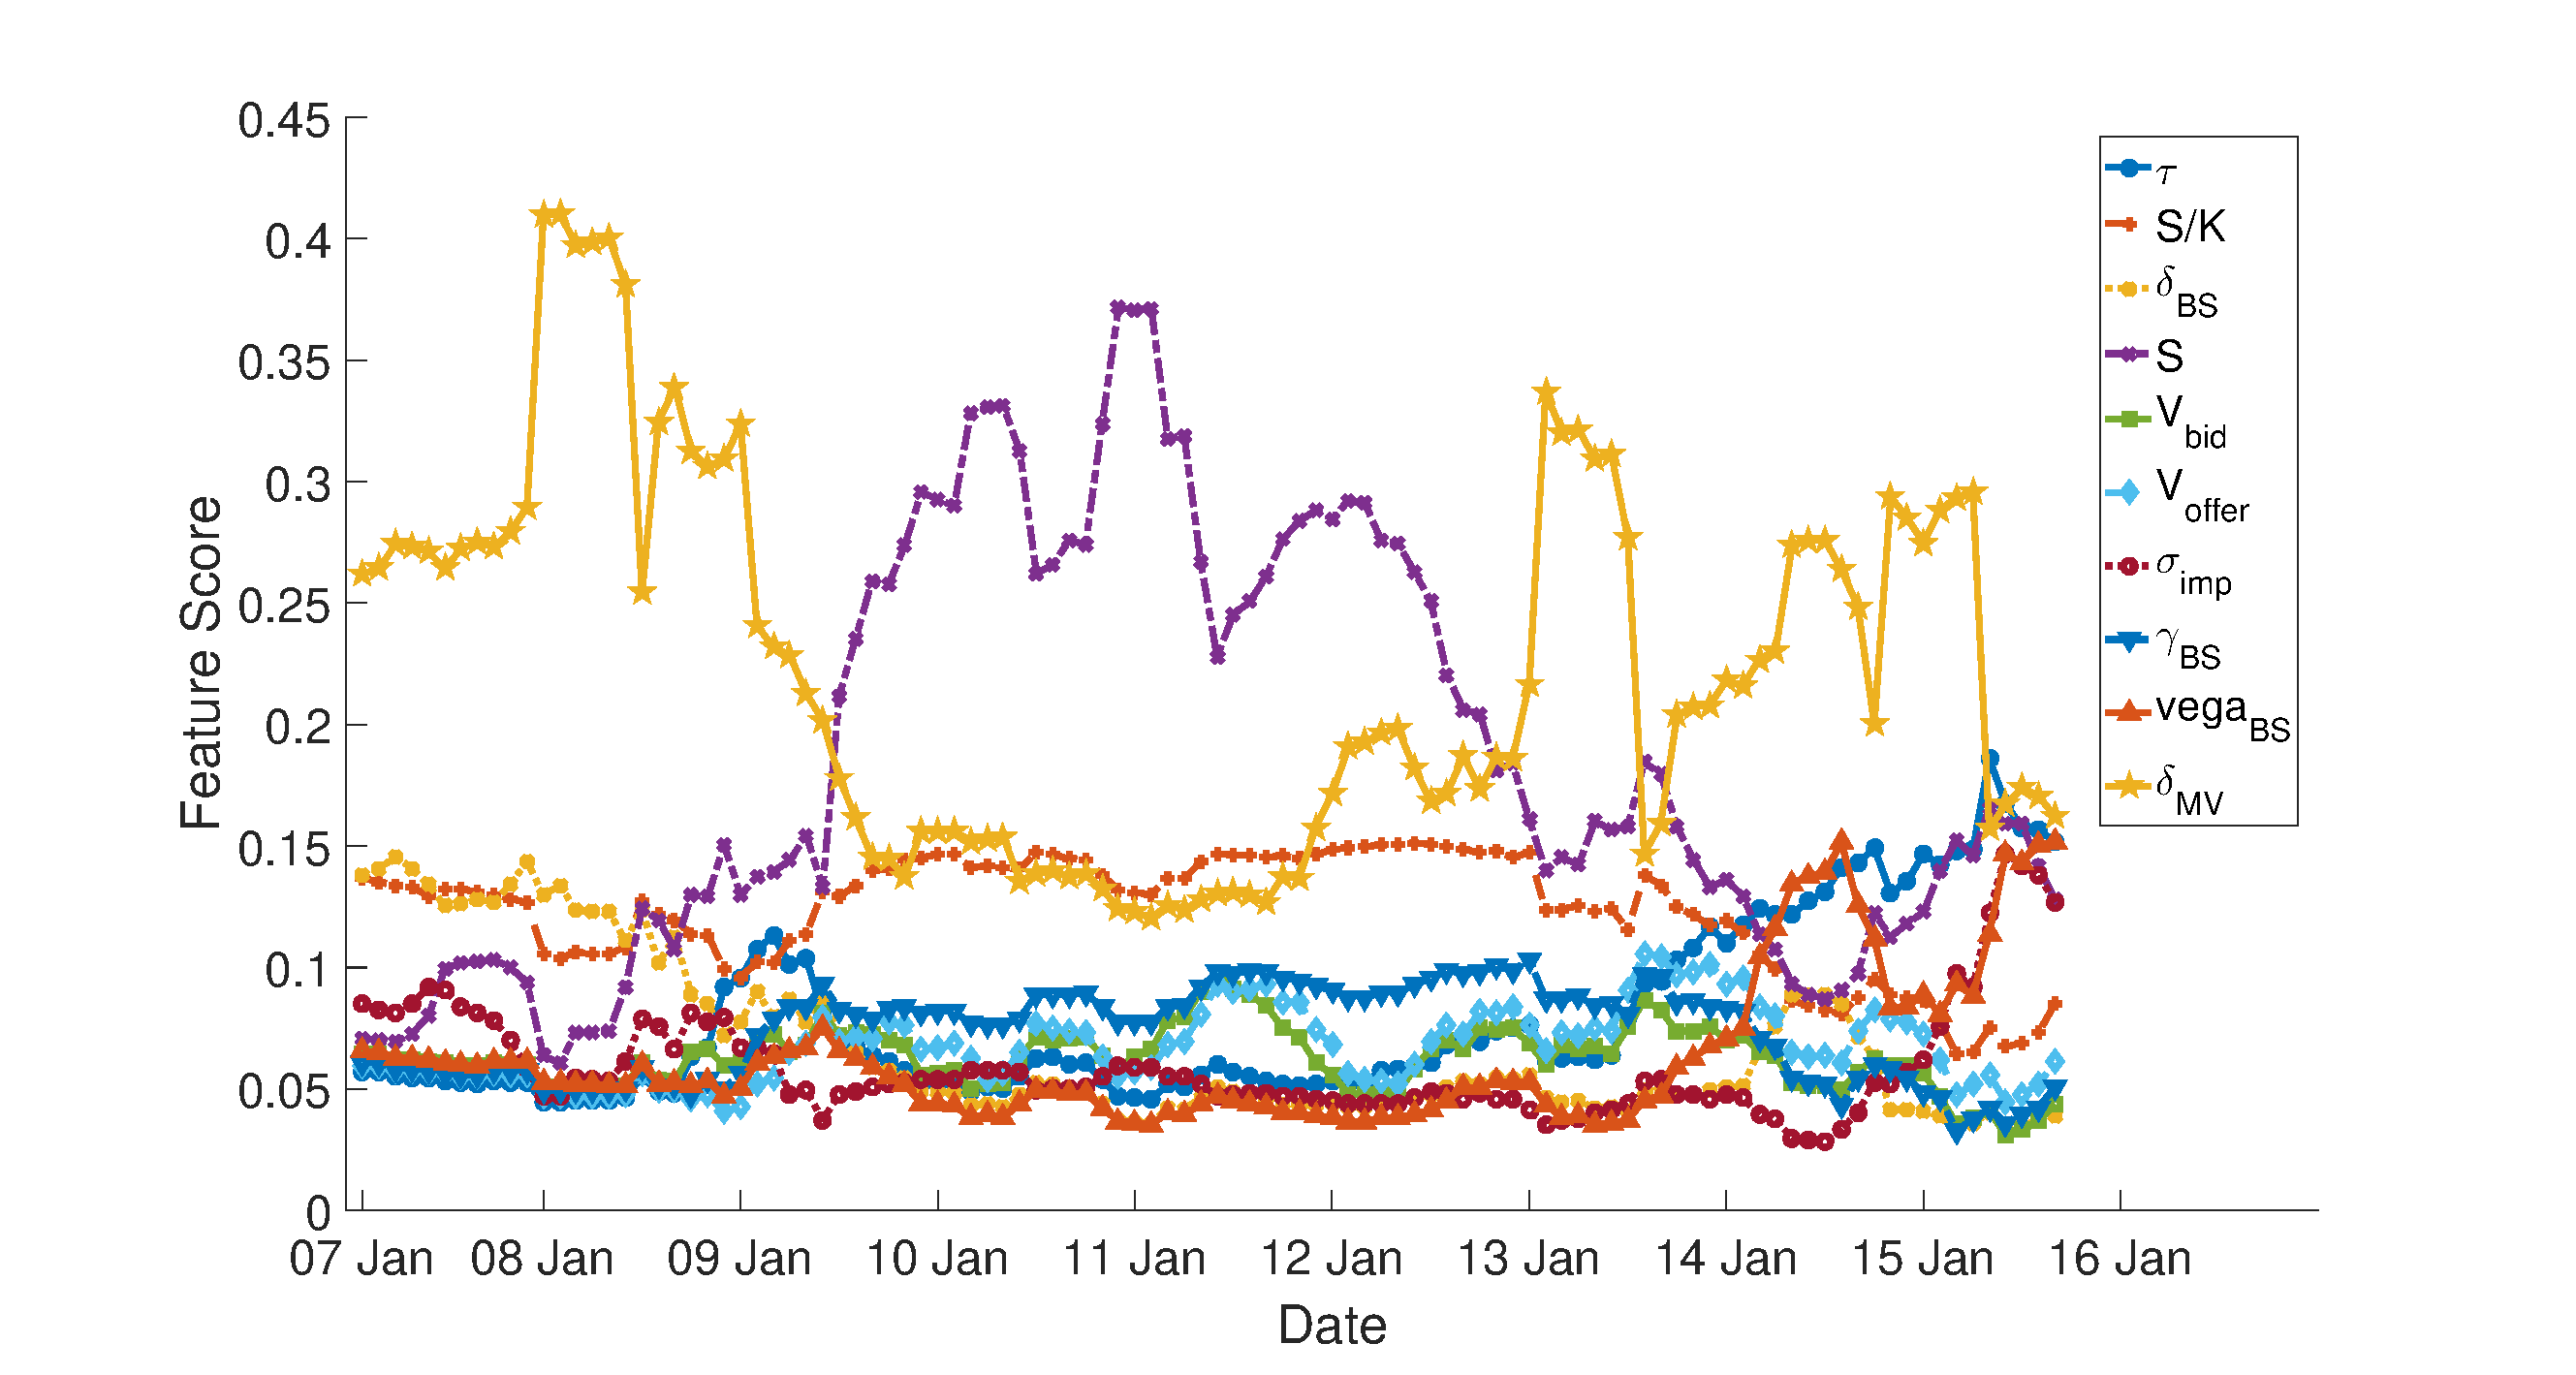
\includegraphics[width=0.48\textwidth]{CLocal0}}
% \subfigure[Sequential Features Daily Hedging]{
%   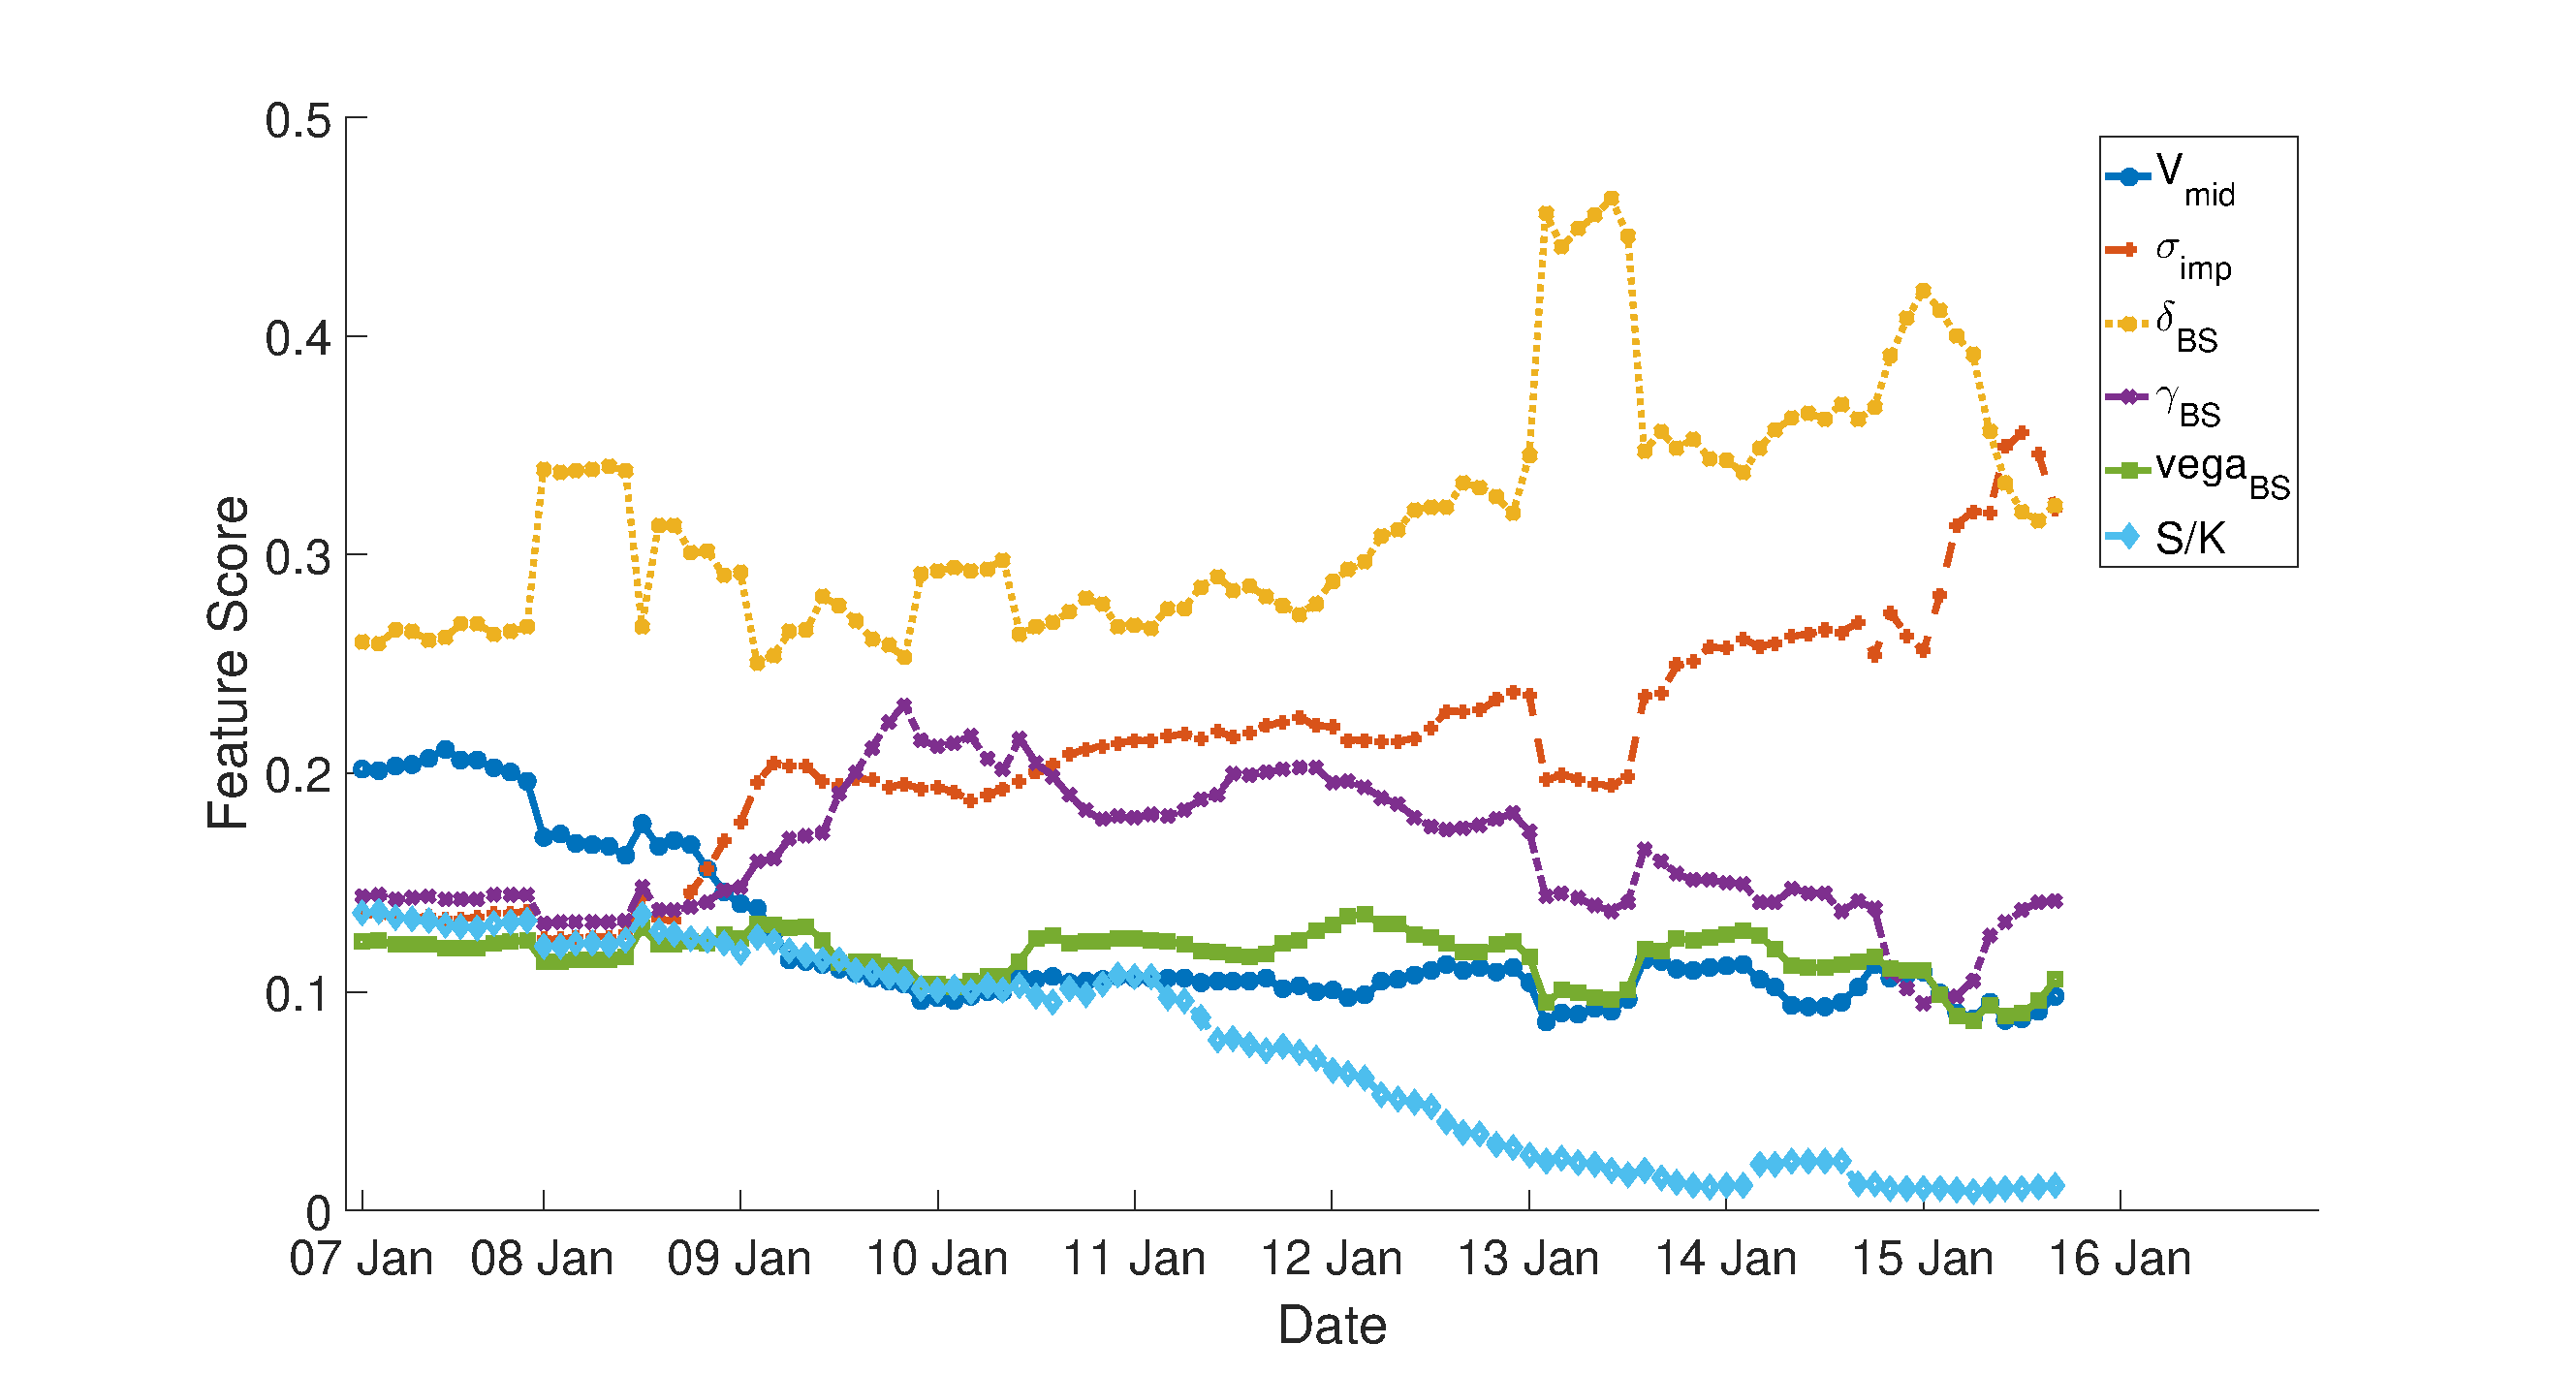
\includegraphics[width=0.48\textwidth]{C0}}
\subfigure[Local Features Weekly Hedging]{
	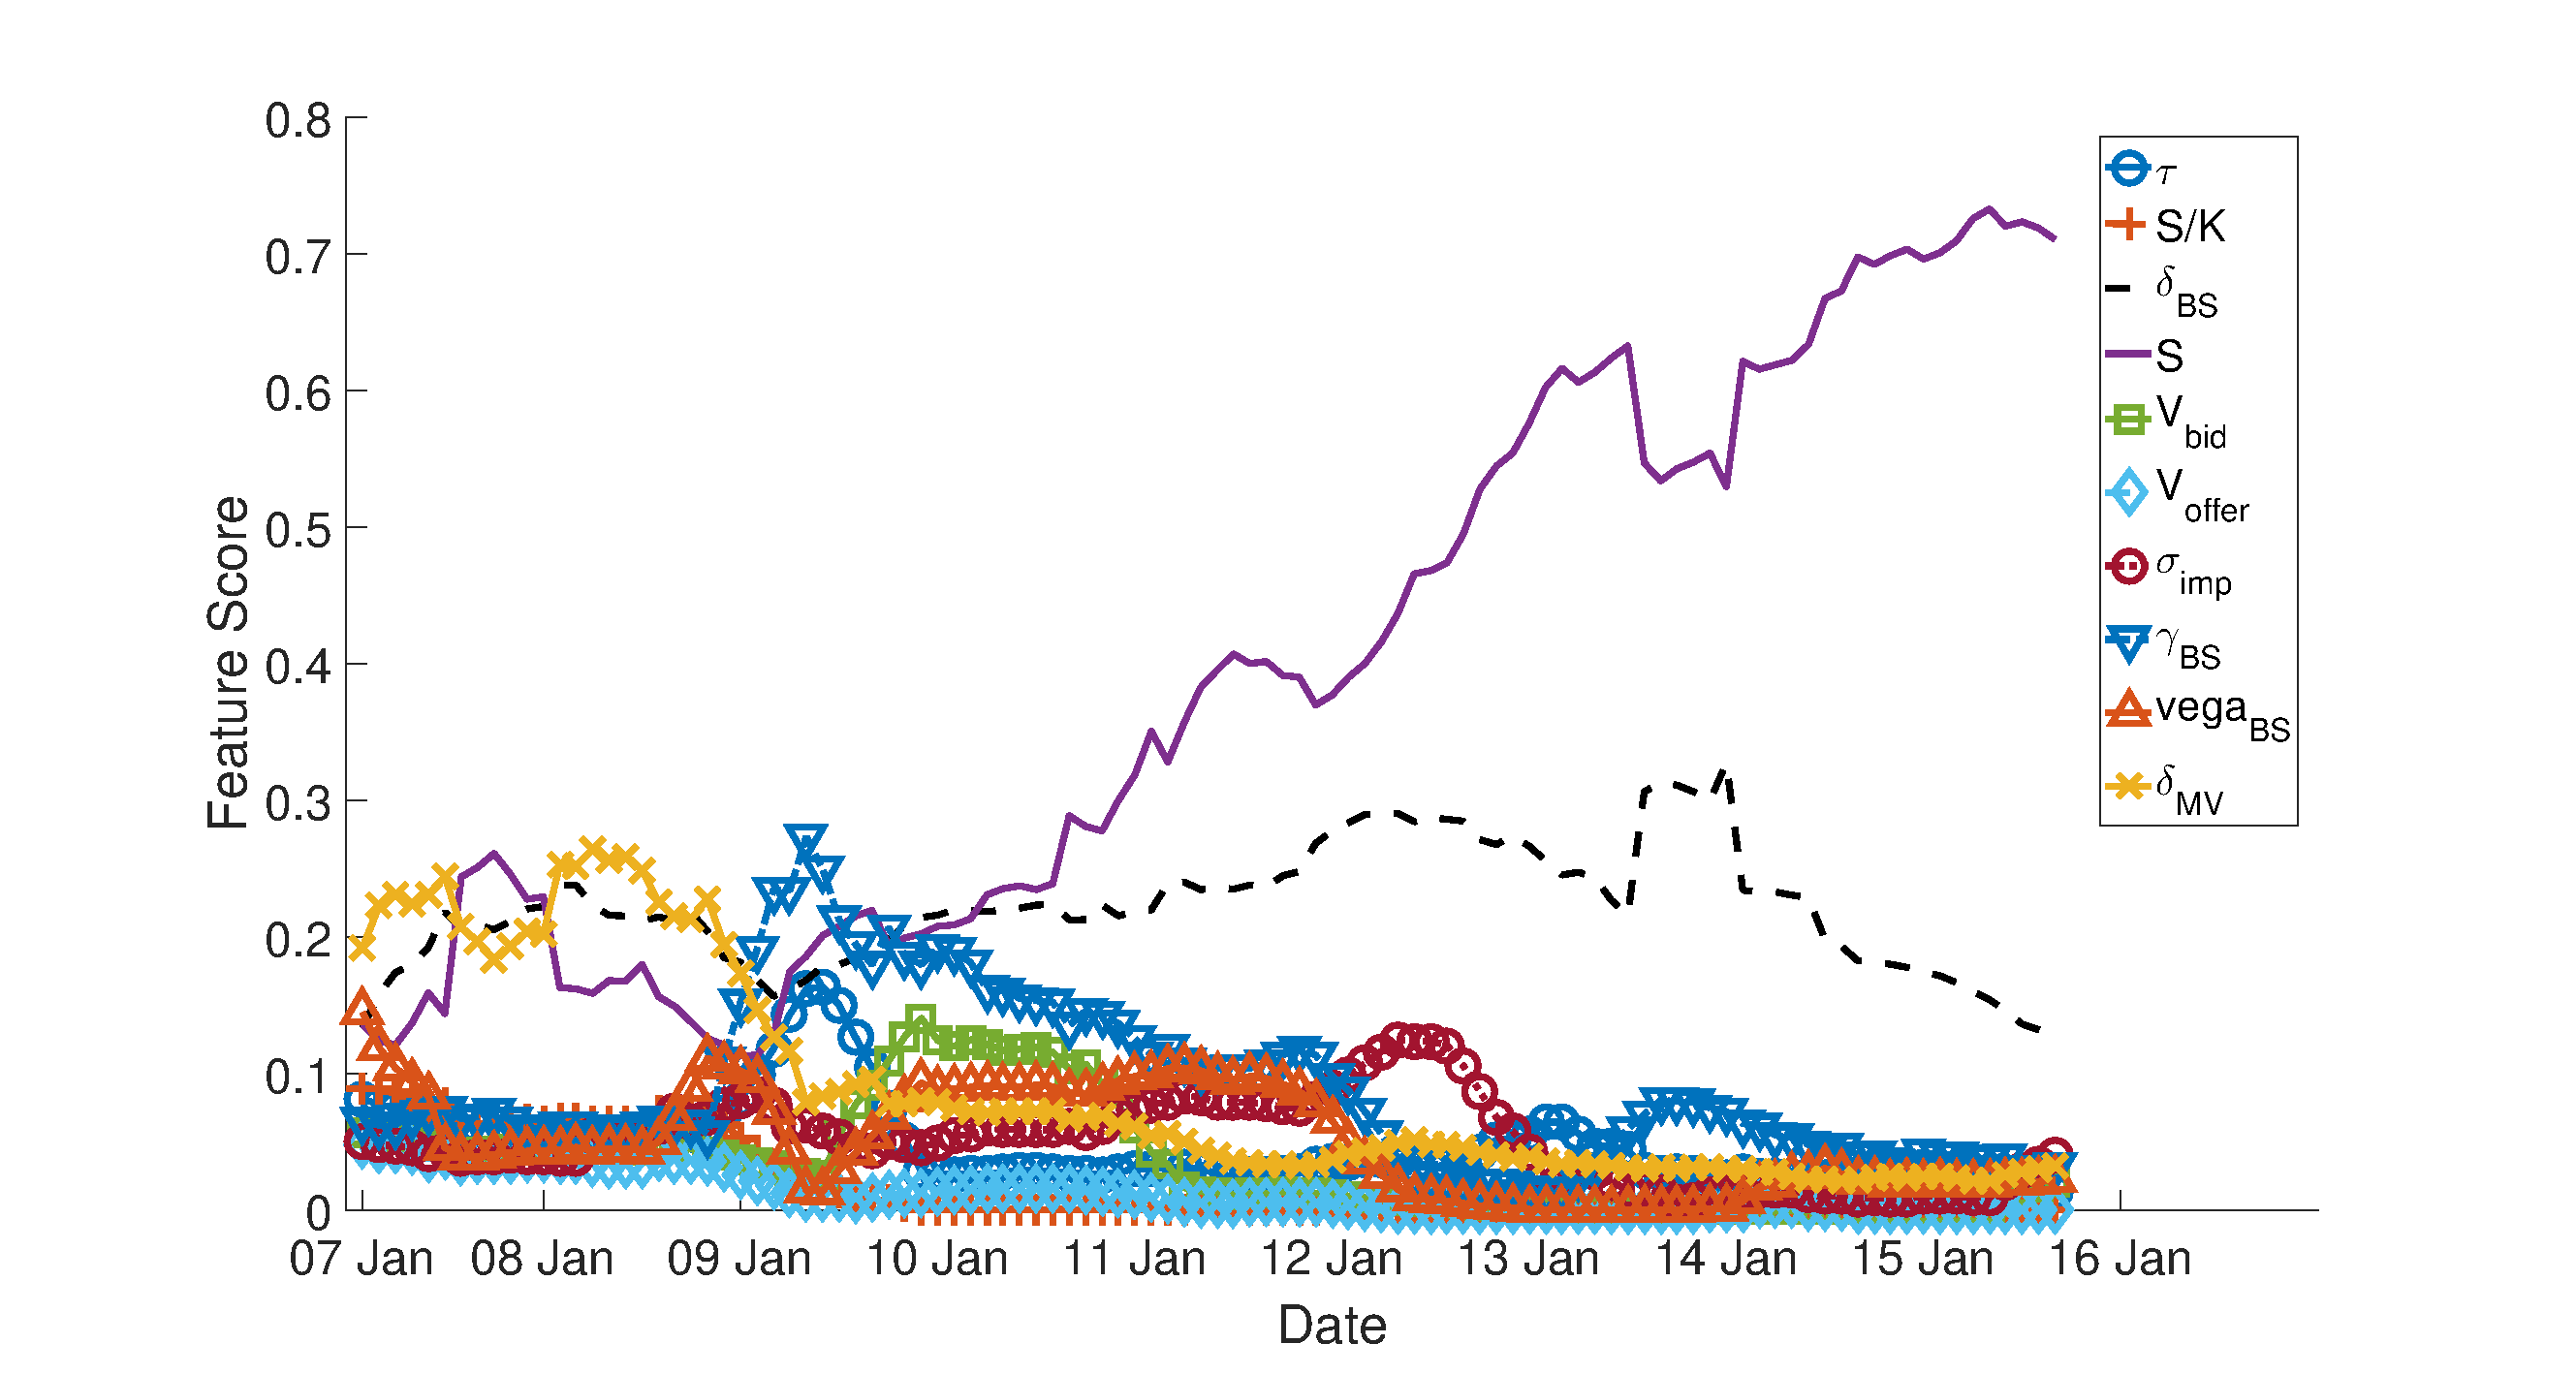
\includegraphics[width=0.48\textwidth]{./figures/CLocal1}}
\subfigure[Sequential Features Weekly Hedging]{
	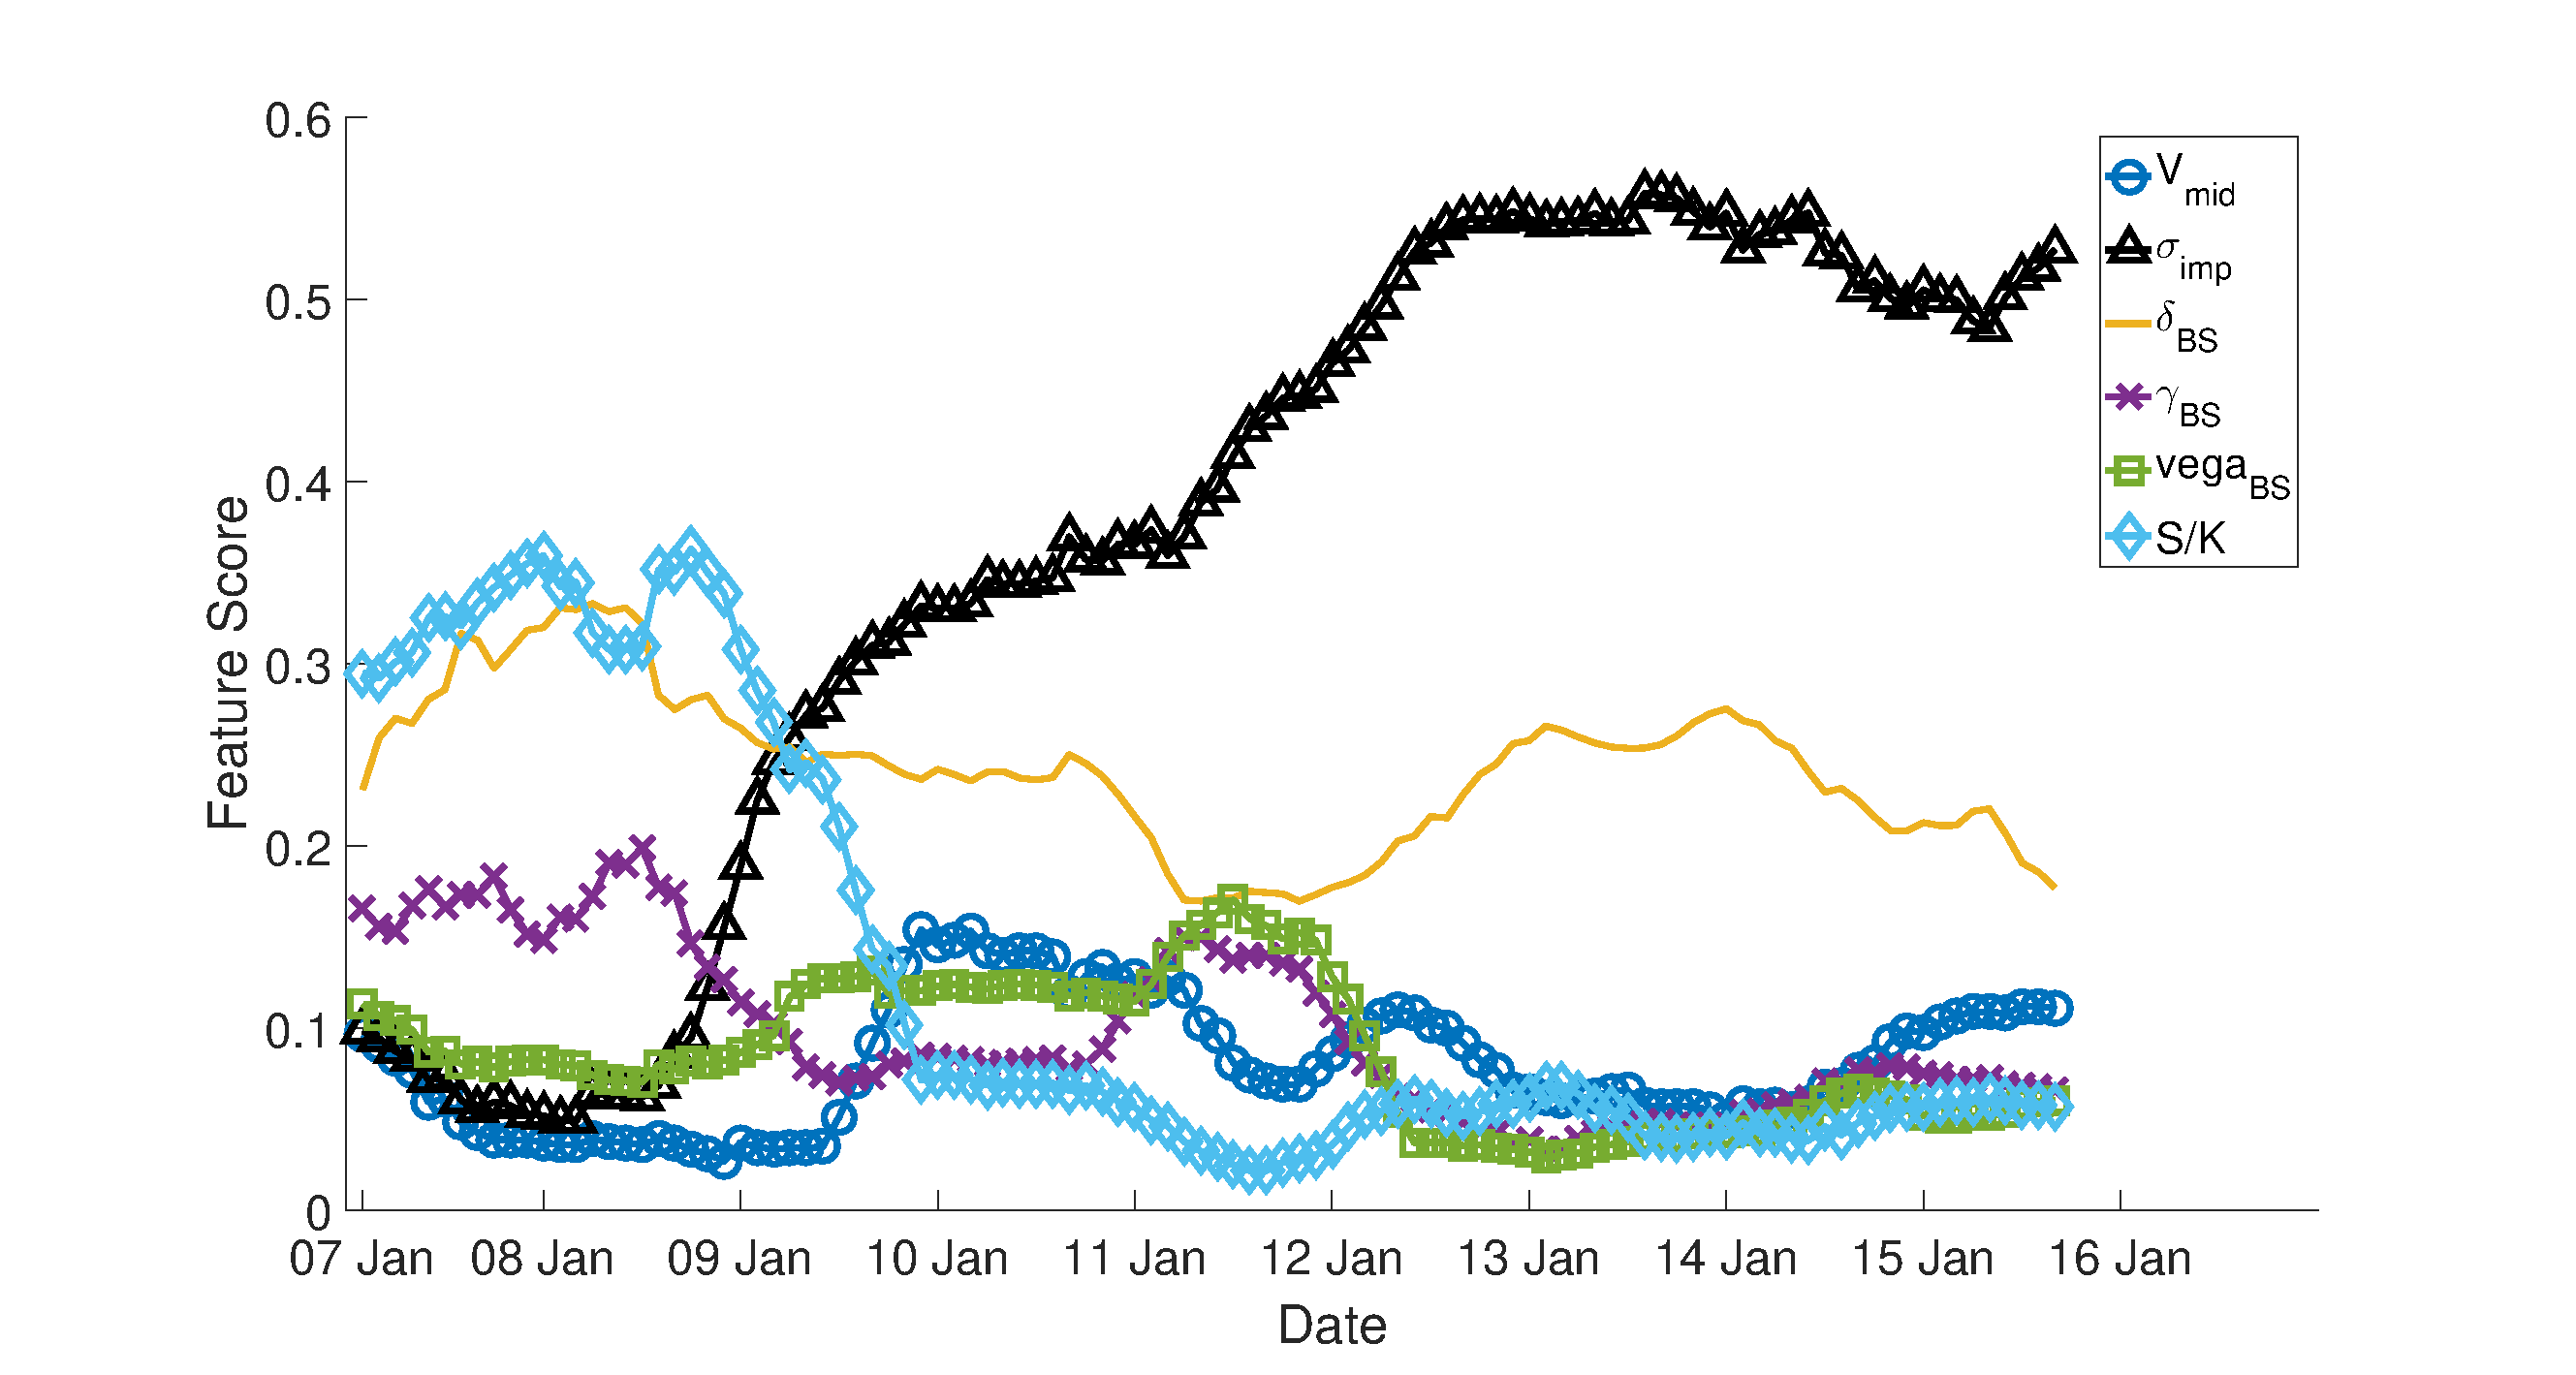
\includegraphics[width=0.48\textwidth]{./figures/C1}}
\subfigure[Local Features Monthly Hedging]{
	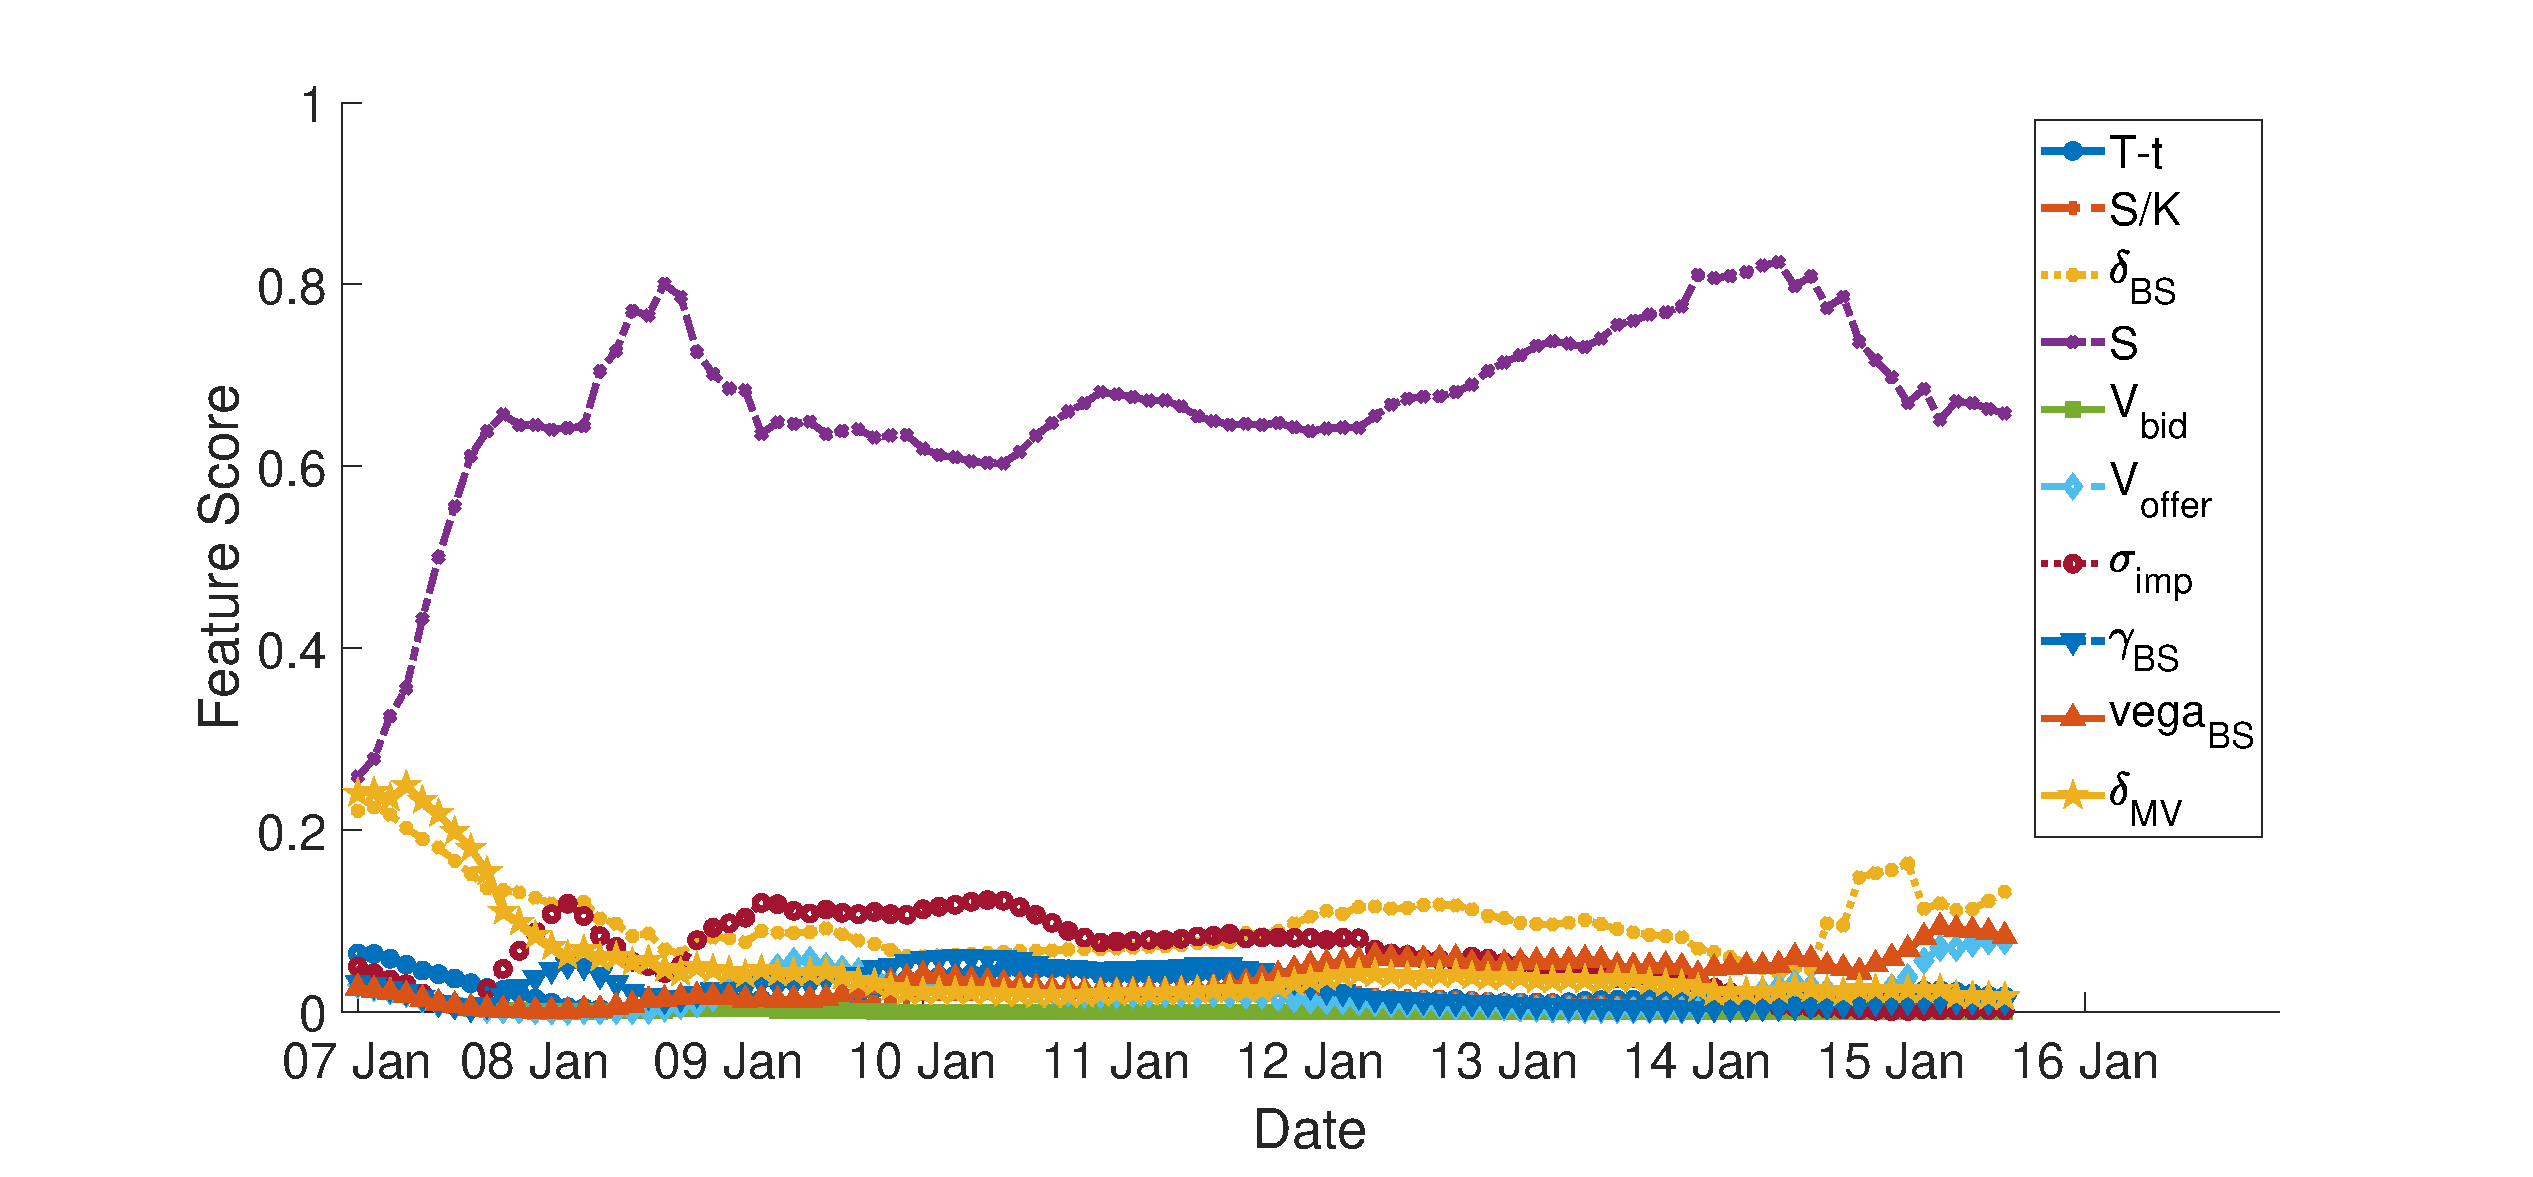
\includegraphics[width=0.48\textwidth]{./figures/CLocal2}}
\subfigure[Sequential Features Monthly Hedging]{
	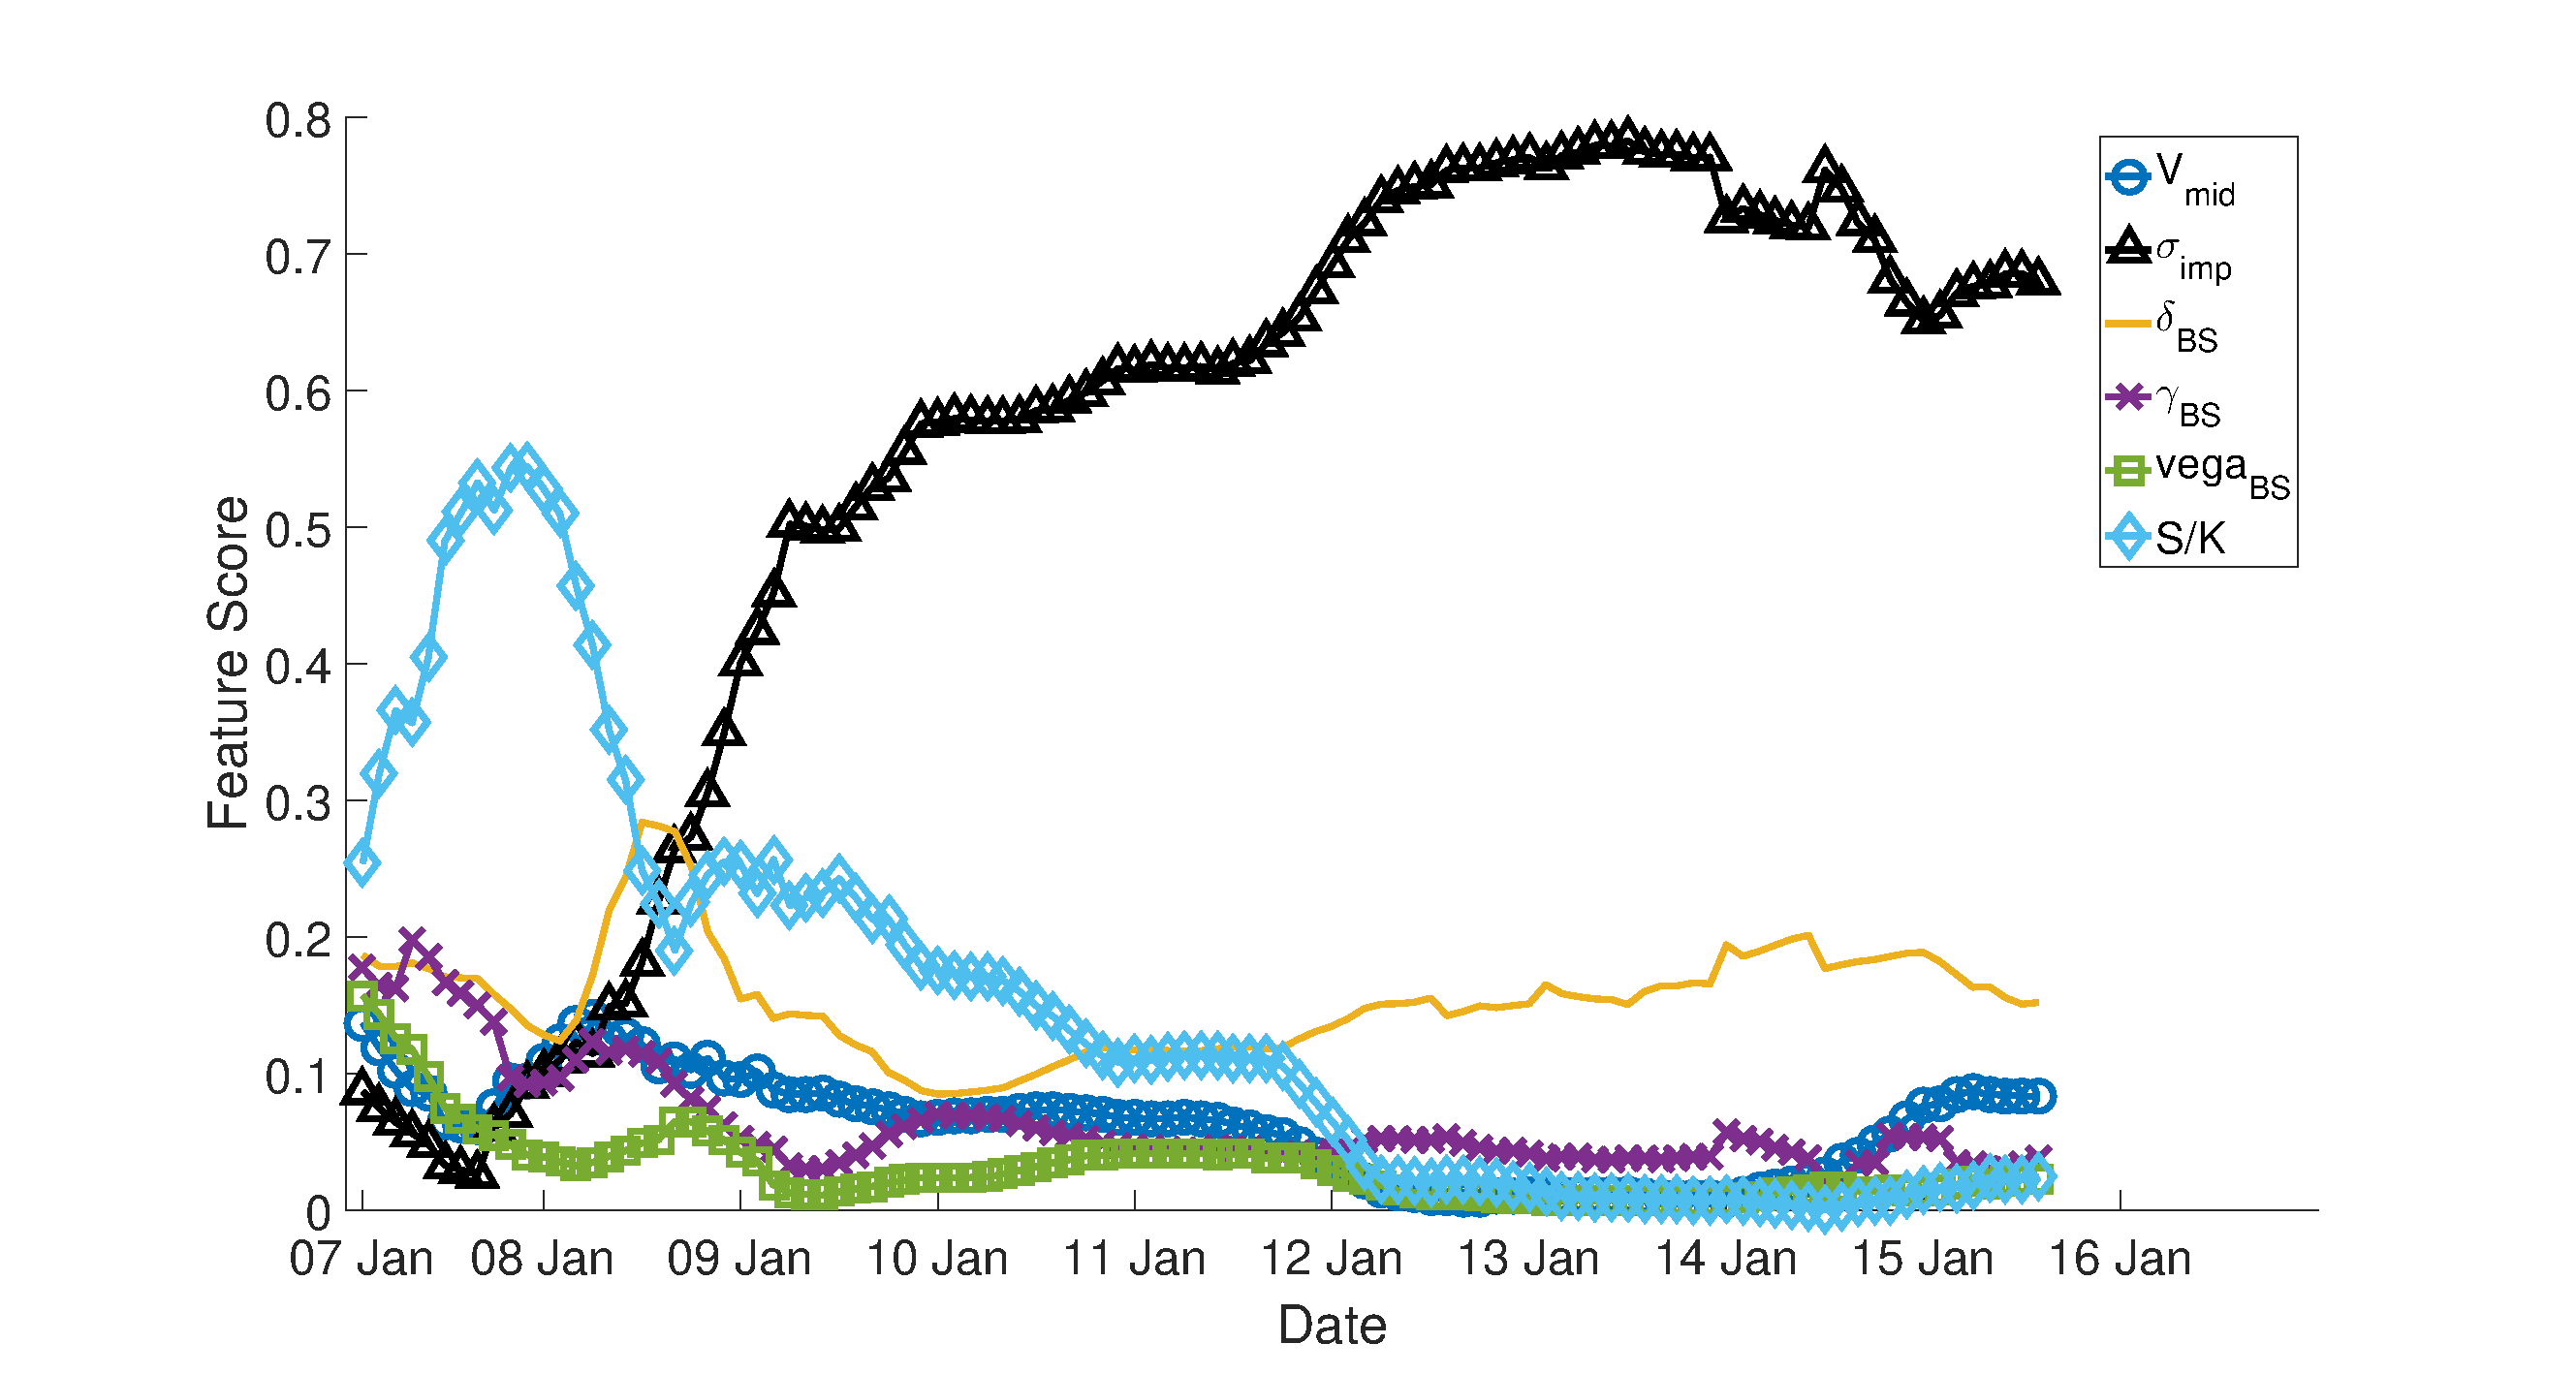
\includegraphics[width=0.48\textwidth]{./figures/C2}}
\caption{Feature scores for weekly and monthly hedging models $\model$ on  traded S\&P500 call option  data.} \label{fig:call1}
\end{figure}





From subplots (a) and (b) in Figure \ref{fig:call1}, it can be observed that, for weekly hedging  call options, the index price $S$ is ranked as the most important local feature after Jan 2010.
Moreover, the average weight for the index price  $S$ exhibits an increasing trend after Jan 2009.
The past implied volatility sequence is ranked as the most important sequential feature after March 2009. The average weight for the past implied volatility sequence also exhibits an increasing trend after Jan 2009. From subplots (c) and (d) in Figure \ref{fig:call1}, it can be observed that, for monthly hedging  the call option, the index price $S$ is always ranked as the most important local feature. In addition, the average weight of the index price  $S$ is always higher than 0.5 after Jan 2008.
The past implied volatility sequence is always ranked as the most important sequential feature after Jan 2009. The average weight for the past implied volatility sequence also is always greater than 0.4 after Jan 2008.

For the put option, the situation is slightly different. From subplots (a) and (b) in Figure \ref{fig:put1}, we can see that, for weekly hedging the put option, the index price $S$ is often ranked as the most important local feature. The past implied volatility sequence and the past BS delta sequence are identified as the two most important sequential features. From subplots (a) and (b) in Figure \ref{fig:put1}, we can see that, for monthly hedging put options, the index price $S$ is ranked as the most important local feature after Jan 2008. The past implied volatility sequence is ranked as the most important sequential feature after Jan 2013.

Overall, the index price $S$ has often been identified as an important local feature for hedging  both call and put options. Since the BS delta of the implied volatility is one of the local features, this confirms the fact that the BS delta does not capture all dependence on the underlying
In addition, the past implied volatility has often been identified as an important sequential feature for hedging both calls and puts.

\begin{figure}[htp]
\centering
%\subfigure[Local Features Daily Hedging]{
%    \includegraphics[width=0.48\textwidth]{PLocal0}}
%\subfigure[Sequential Features Daily Hedging]{
%    \includegraphics[width=0.48\textwidth]{P0}}
\subfigure[Local Features Weekly Hedging]{
	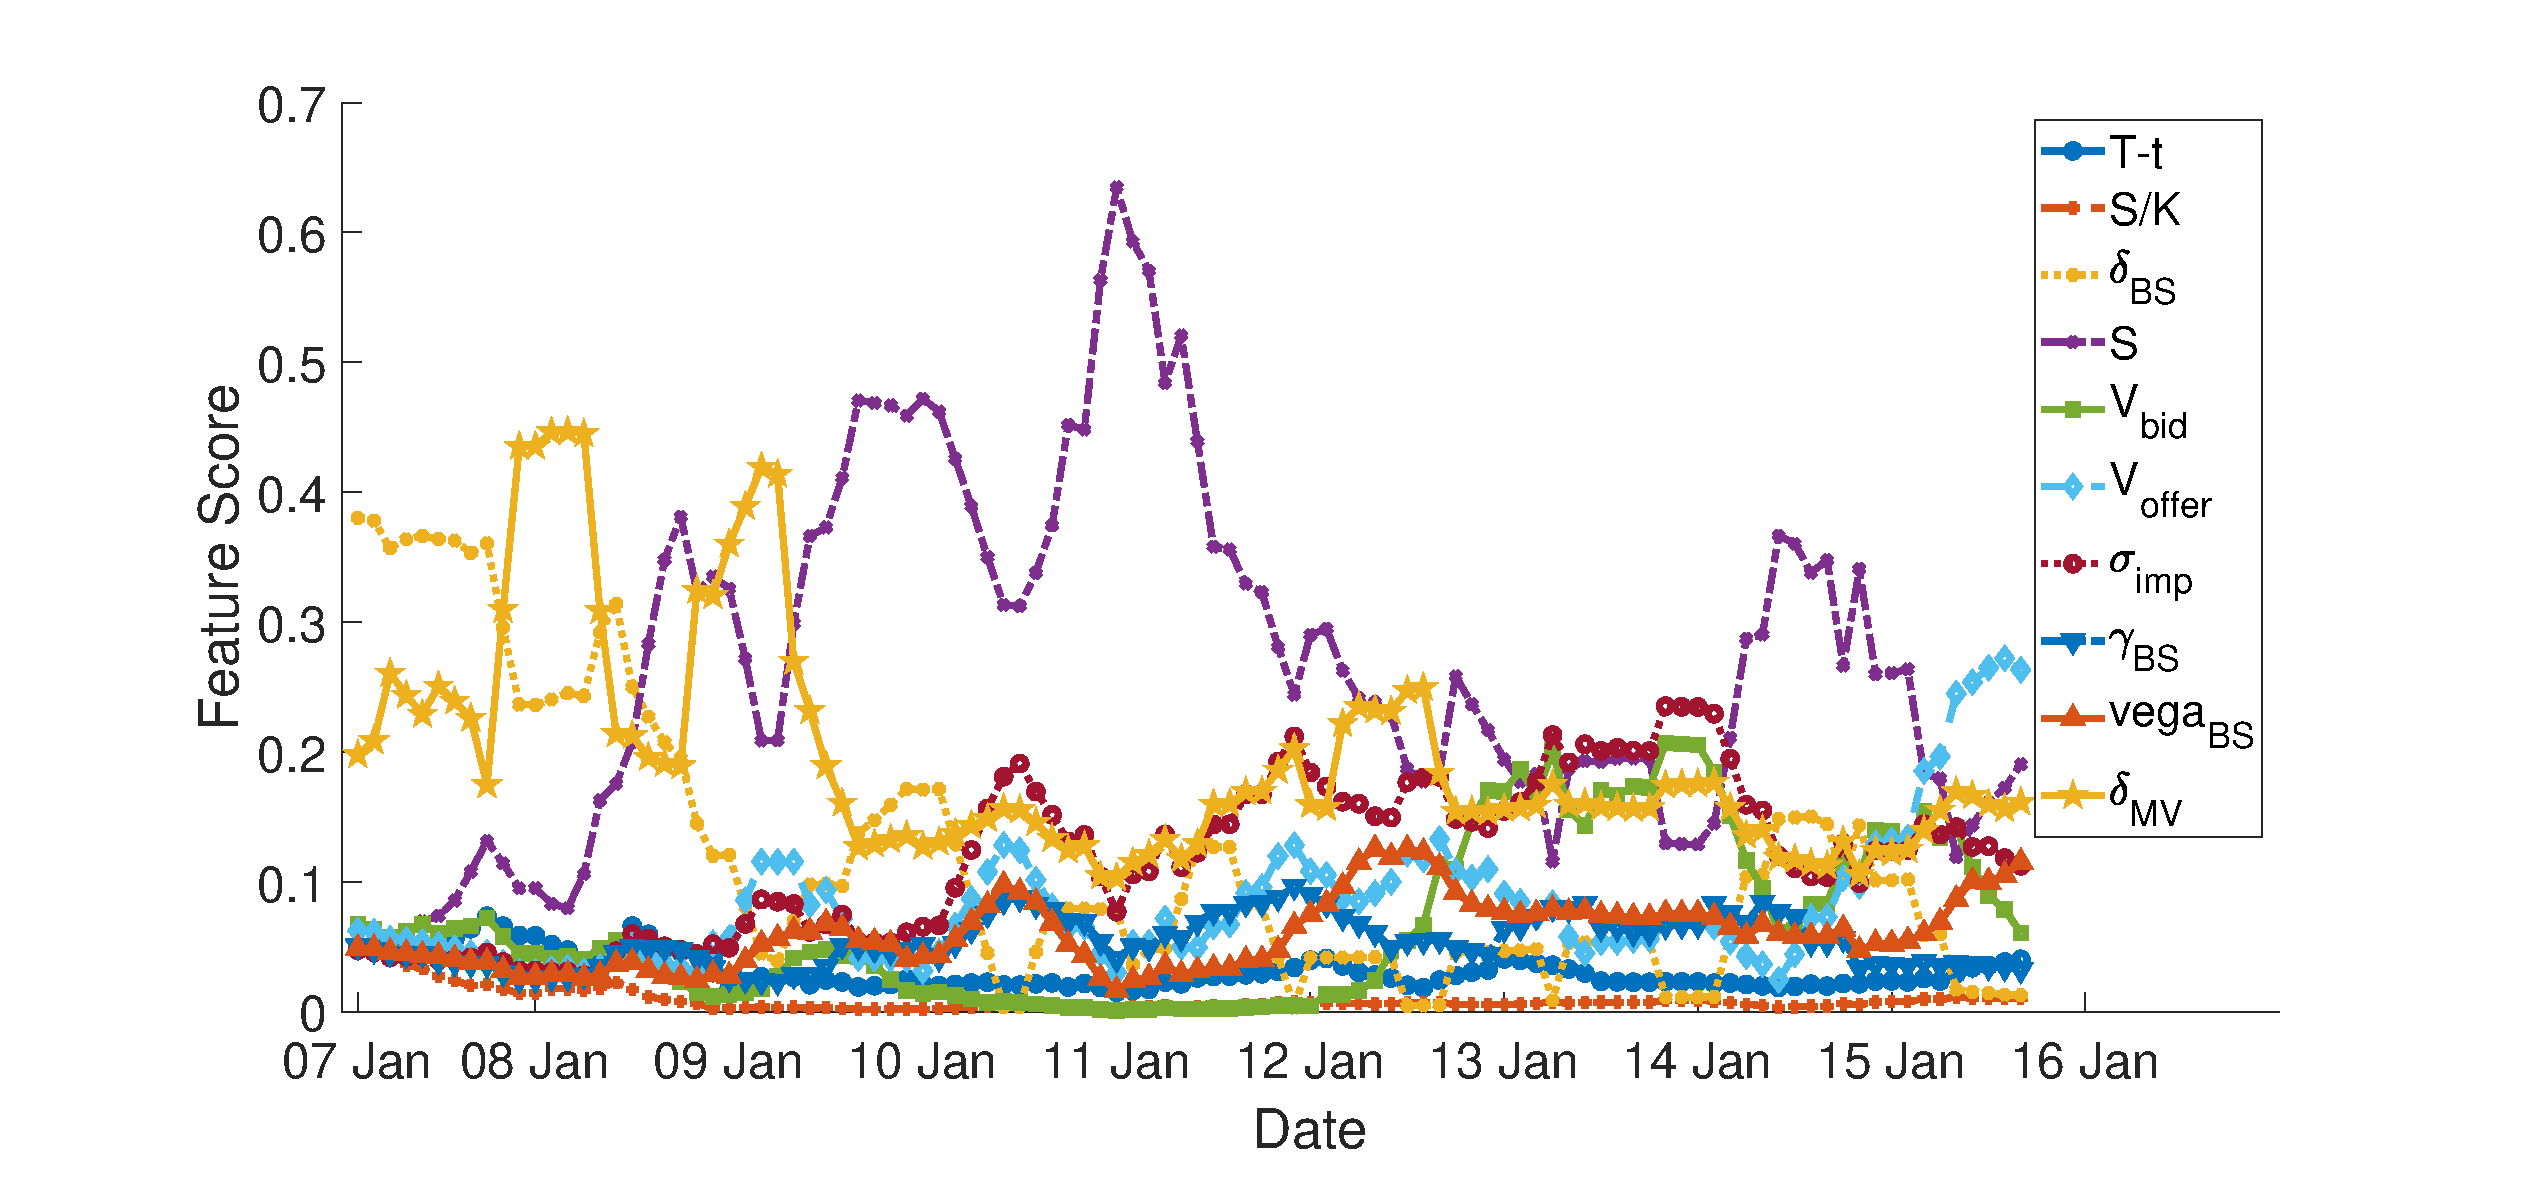
\includegraphics[width=0.48\textwidth]{./figures/PLocal1}}
\subfigure[Sequential Features Weekly Hedging]{
	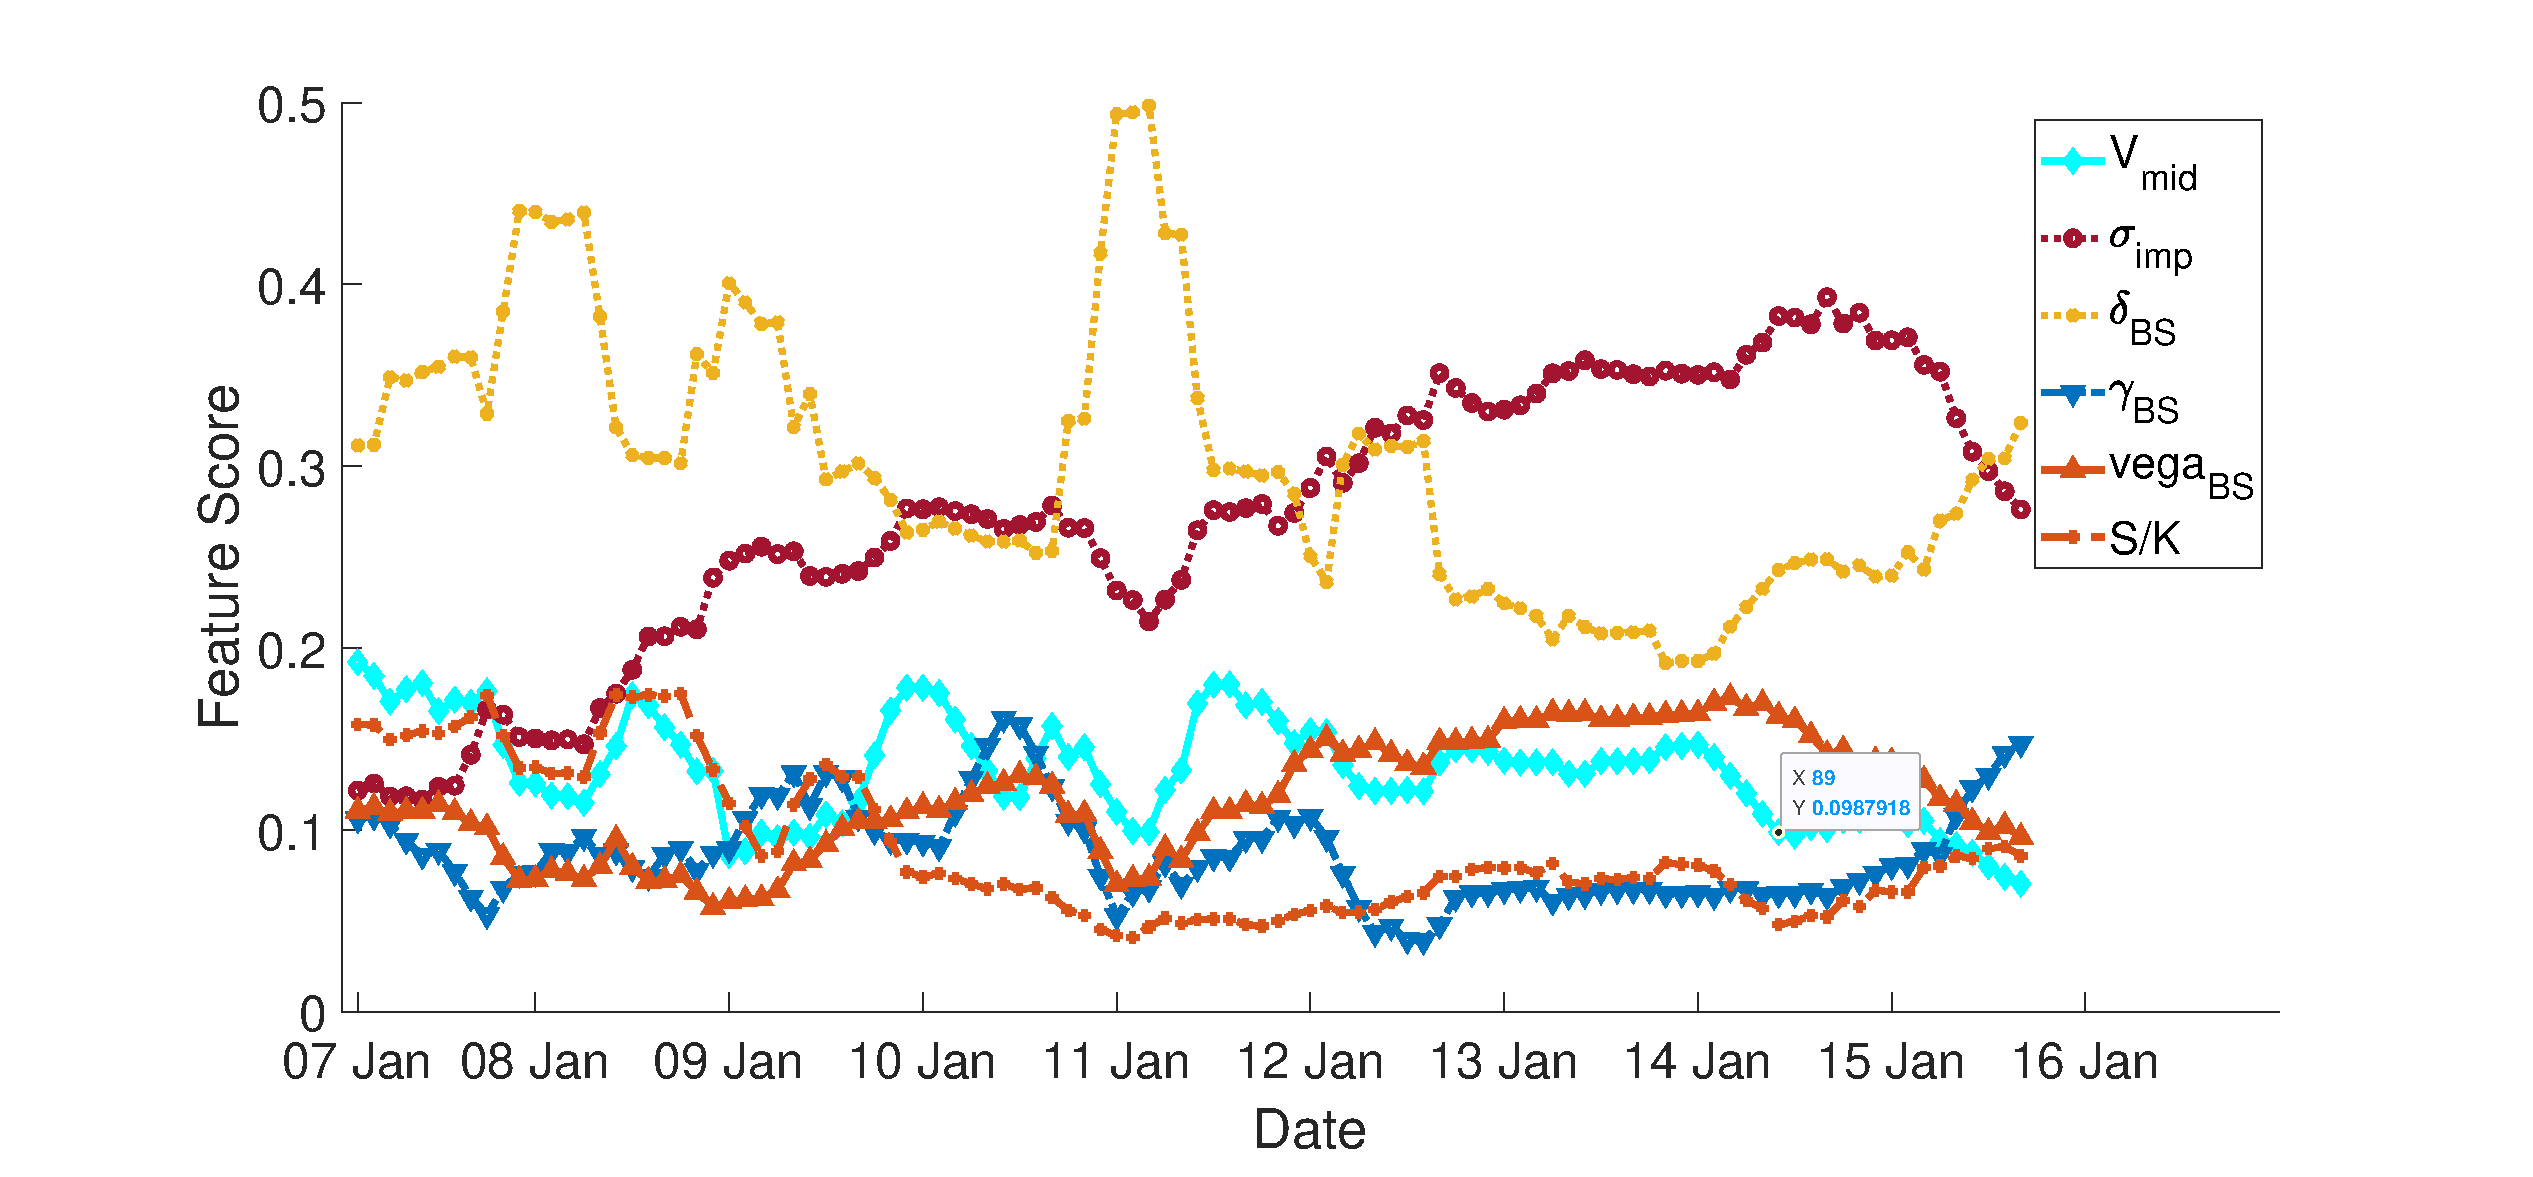
\includegraphics[width=0.48\textwidth]{./figures/P1}}
\subfigure[Local Features Monthly Hedging]{
	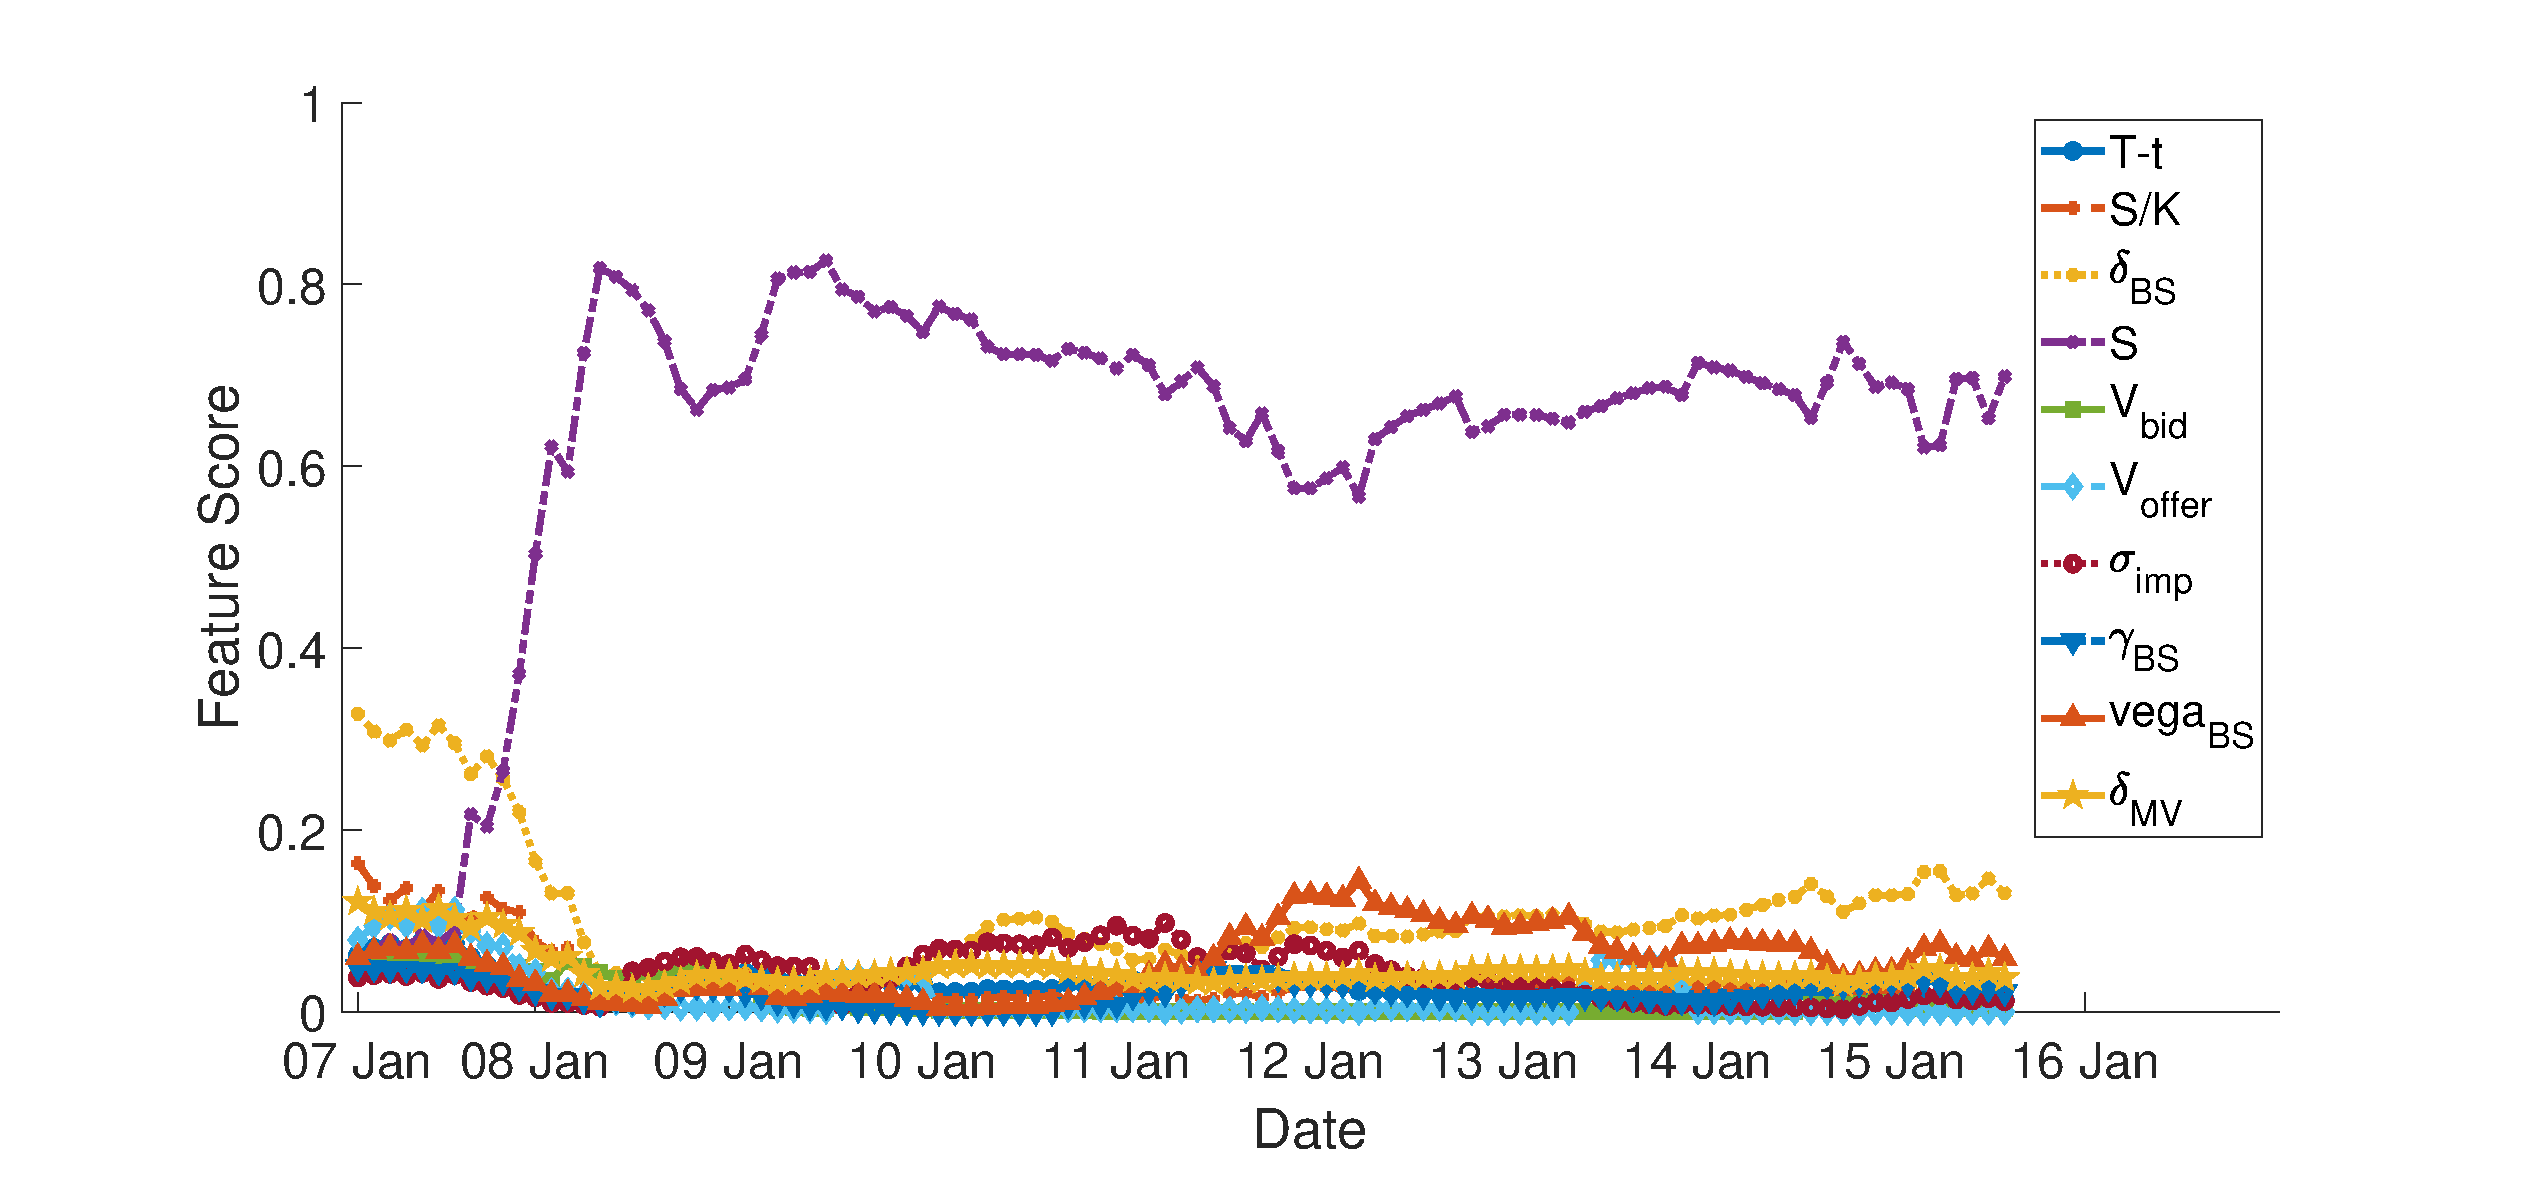
\includegraphics[width=0.48\textwidth]{./figures/PLocal2}}
\subfigure[Sequential Features Monthly Hedging]{
	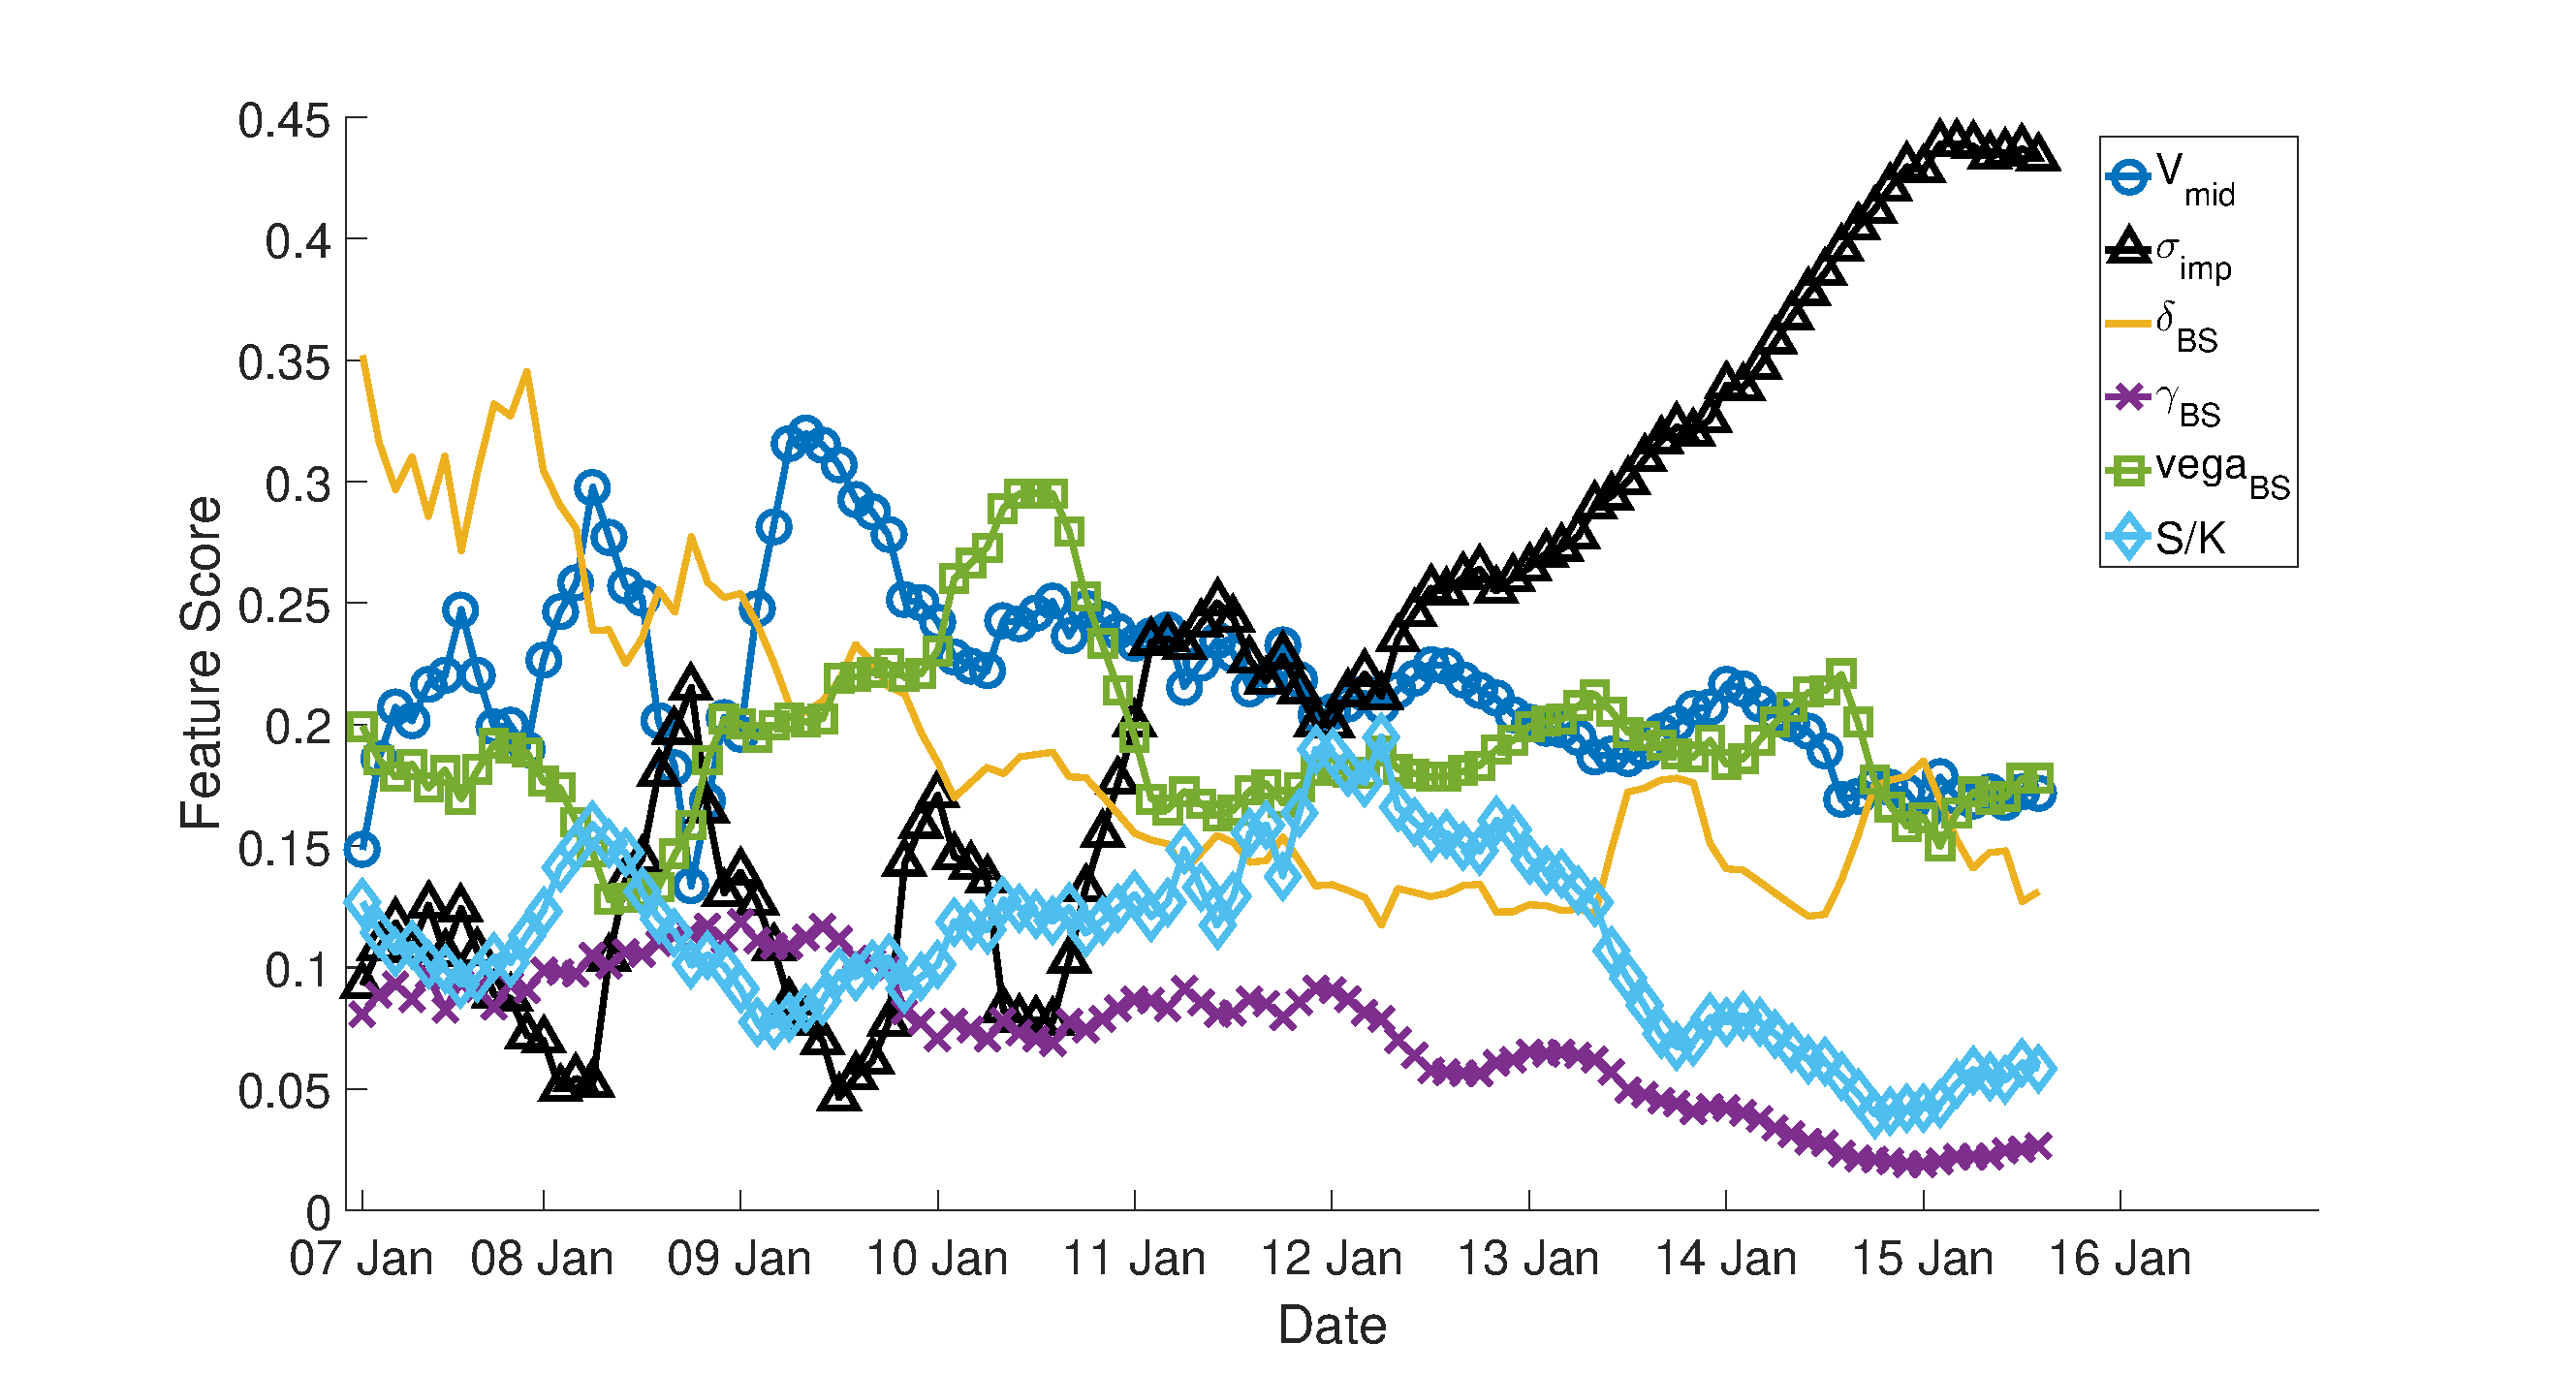
\includegraphics[width=0.48\textwidth]{./figures/P2}}
\caption{Feature score for weekly and monthly hedging models $\model$ on traded S\&P500 put option  data} \label{fig:put1}
\end{figure}

\subsection{Daily Hedging Comparison}\label{sec:daily}
In section \ref{sec:weekly} - \ref{sec:featureWeek}, we have have presented hedging comparisons for weekly and monthly hedging. Now we compare the proposed $\model$  with the following methods for daily hedging,
\iffalse
Also, the decoder only model significantly improves over the regularized kernel model $\DKLs$. This improvement comes partly from the daily model updating (which is computationally feasible for the proposed $\model$)  while $\DKLs$ is updated monthly only (due to computational cost and the length of the study period).
\fi


\begin{itemize}
	\item $\MV$: MV hedging   based on formulation \eqref{eq:HullWhite},
\item ${\LVF}$: MV hedging in \cite{hulloptimal} from local volatility function based on formulation \eqref{eq:HullWhiteLVF},
\item ${\SABR}$ : MV hedging in  \cite{hulloptimal} from {{SABR}} model based on formulation \eqref{eq:HullWhiteSabr},
\item ${\delta^{BS}}$:  implied  volatility Black–Scholes delta,
\item Bartlett: Bartlett formula based on \eqref{eq:bartlett},
  \item $\DKLs$: Direct spline kernel hedging method as in \ref{sec:KernelDirect}.
\end{itemize}

We have omitted  $\modelN$ and $\textsc{GRU}_{c}$ in the daily hedging comparison since it has been shown to underperform $\model$. But we  have added ${\LVF}$ and ${\SABR}$ since they are based on instantaneous hedging analysis and are more suitable for daily hedging.

%In the following discussion, we use $\model$  to denote the proposed $\model$ in Figure \ref{fig:RNNModel}.
Since the  same S\&P 500 index option data from the OptionMetric Database is used here,  we simply quote the results  presented in \cite{hulloptimal} for  $\MV$,  ${\LVF}$,  and ${\SABR}$, and the results  presented in \cite{knian2017} for  $\DKLs$.

As stated in \cite{hulloptimal} and section \ref{sec:Classical},
the ${\SABR}$ model is calibrated daily, from which the hedge position is determined and applied the next day.
For  ${\LVF}$, the partial derivative of the expected implied volatility to the underlying is calculated from the slope of the observed implied volatility smile daily.  For $\MV$, the model parameter, $a,b \text{ and } c$ are estimated using all options in a 36-month-window and then applied to determine the hedging position daily in the subsequent month.
%We refer interested readers to \citep{hulloptimal} for more details of how  ${\SABR}$,${\LVF}$ and $\MV$ are calibrated and implemented.


Table \ref{SP500Call} presents daily hedging comparisons for call options.
From  Table \ref{SP500Call}, using either {traded} data or {all} data for testing, $\model$  outperforms the minimum variance hedging methods reported in \cite{hulloptimal} in the overall performance.   For most delta buckets, delta greater than or equal to 0.3, the performance of  $\model$  is better than those of the minimum variance hedging methods. However, for the bucket of the delta value 0.1 or 0.2, the performance is slightly worse.


%Secondly, we compare the hedging performance from the direct kernel hedging $\DKLs$ method and the proposed $\model$ method.
In addition, from Table \ref{SP500Call}, the performance of the $\model$ model is slightly better than that of the kernel hedging $\DKLs$ in overall performance. For the the delta buckets 0.3-0.9,  $\model$ outperforms the direct kernel hedging $\DKLs$.  However,  $\model$ performs slightly worse for the delta bucket 0.1 and 0.2.

Table \ref{SP500Put}  presents daily hedging comparisons for put options.
Table \ref{SP500Put} shows that both overall performance and the performances for different delta buckets of the $\model$ model are better than those from minimum variance hedging methods in \cite{hulloptimal} and the direct kernel hedging $\DKLs$, for testing result using all data. Similarly to the call, $\model$ has model bold entries in most of delta buckets, indicating outperforming other methods.
\iffalse
For the testing result using only traded data, the overall results from $\model$ are better than results reported from the minimum variance hedging methods in \cite{hulloptimal} and from the direct kernel hedging $\DKLs$.  As for the testing results with traded data, in different buckets, the performances of $\model$ for delta buckets -0.9, -0.8 and -0.1 are slightly worse than those from the minimum variance hedging methods in \cite{hulloptimal} and the direct kernel hedging $\DKLs$,  while  the performance of the $\model$ method for the other delta bucket is  better or similar.
\fi

 Both $\model$ and $\DKLs$ are non-parametric data-driven hedging  methods, with a main difference in features included. The hedging performance comparison between the two suggests that including the sequential features and more local features improves the overall hedging performance slightly for daily hedging.



\begin{table}[htp!]
\centering
\begin{threeparttable}
\begin{tabular}{|c |r r r r r r r r r|}
\hline
\multirow{3}{*}{Delta}&\multirow{3}{*}{MV (\%)}&\multirow{3}{*}{\;$\SABR$(\%)}&\multirow{3}{*}{\LVF (\%)}&\multicolumn{2}{c|}{Bartlett}& \multicolumn{4}{c|}{Data-Driven Model}\\
&&&&\multirow{2}{*}{Traded}&\multirow{2}{*}{All}&\multicolumn{2}{|c}{$\DKLs$ (\%)} &\multicolumn{2}{c|}{$\model$ (\%)}\\
&&&&&&\multicolumn{1}{|c}{\small Traded}&\multicolumn{1}{c}{\small All}&\multicolumn{1}{c}{\small Traded}&\multicolumn{1}{c|}{\small All}\\ \hline
  0.1 & 42.1 & 39.4 & 42.6 &29.0 &35.1    & 47.1  & 48.6        &32.3          &   33.8        \\
  0.2 & 35.8 & 33.4 & 36.2 &28.2 &32.3    & 37.8  & 40.0        &33.7          &   36.4        \\
  0.3 & 31.1 & 29.4 & 30.3 &27.7 &28.9   & 34.1  & 35.1        &34.1          &\textbf{35.5}        \\
  0.4 & 28.5 & 26.3 & 26.7 &28.7 &27.3   & 32.3  & 32.0        &\textbf{33.7} &\textbf{34.2}    \\
  0.5 & 27.1 & 24.9 & 25.5 &26.9 &26.7   & 29.3  & 29.4        &\textbf{35.1} &\textbf{33.0}   \\
  0.6 & 25.7 & 25.2 & 25.2 &28.3 &26.6   & 29.9  & 28.4        &\textbf{35.6} &\textbf{32.1}    \\
  0.7 & 25.4 & 24.7 & 25.8 &28.5 &26.4   & 29.0  & 26.8        &\textbf{31.8} &\textbf{29.7}   \\
  0.8 & 24.1 & 23.5 & 25.4 &23.1 &24.9   & 25.9  & 24.7        &\textbf{28.6} &\textbf{26.5}   \\
  0.9 & 16.6 & 17.0 & 16.9 &14.0 &15.6   & 17.7  & 13.9        &\textbf{19.3} &\textbf{18.9}    \\
  Overall & 25.7 & 24.6 & 25.5 &27.1 &24.8 & 31.3  & 26.0        &\textbf{32.9} & \textbf{28.7} \\
  \hline
\end{tabular}
\caption{S\&P 500 call option hedging for 1-business day: bold entries indicating best Gain from $\model$.  The Gain ratio is a measure for the local hedging performance. The larger the gain ratio is, the better improvement the model achieves over the baseline BS delta hedging method in terms of local hedging risk. The gain ratio is reported on different delta buckets.}
\label{SP500Call}

\end{threeparttable}
\end{table}


\begin{table}[htp!]
\centering
\begin{threeparttable}
\begin{tabular}{|c |r r r r r r r r r|}
\hline
\multirow{3}{*}{Delta}&\multirow{3}{*}{MV (\%)}&\multirow{3}{*}{\;$\SABR$(\%)}&\multirow{3}{*}{\LVF (\%)}&\multicolumn{2}{c|}{Bartlett}& \multicolumn{4}{c|}{Data-Driven Model}\\
&&&&\multirow{2}{*}{Traded}&\multirow{2}{*}{All}&\multicolumn{2}{|c}{$\DKLs$ (\%)} &\multicolumn{2}{c|}{$\model$ (\%)}\\
&&&&&&\multicolumn{1}{|c}{\small Traded}&\multicolumn{1}{c}{\small All}&\multicolumn{1}{c}{\small Traded}&\multicolumn{1}{c|}{\small All}\\ \hline
  			-0.9 & 15.1    &11.2  &-7.4 &9.1  &23.4   &8.6    &13.6  &\textbf{15.1}    &\textbf{17.2} \\
			-0.8 & 18.7    &19.6  &6.8  &3.2  &21.9   &6.5    &16.7  &\textbf{23.2}    &\textbf{28.5} \\
			-0.7 & 20.3    &17.7  &9.1  &1.5  &20.1   &10.6   &19.8  &\textbf{28.5}    &\textbf{32.8} \\
			-0.6 & 20.4    &16.7  &9.2  &6.1  &19.2   &14.9   &21.0  &\textbf{28.3}    &\textbf{33.9} \\
			-0.5 & 22.1    &16.7  &10.8 &15.5 &21.3   &22.5   &23.1  &\textbf{29.2}    &\textbf{34.5} \\
			-0.4 & 23.8    &17.7  &12.0 &21.0 &24.4   &24.2   &25.2  &\textbf{29.9}    &\textbf{34.7} \\
			-0.4 & 27.1    &21.7  &16.8 &26.7 &29.0   &27.7   &28.3  &\textbf{30.6}    &\textbf{33.6} \\
			-0.2 & 29.6    &25.8  &20.6 &29.3 &31.6   &30.1   &30.8  &25.4    &29.9 \\
			-0.1 & 27.5    &26.9  &17.7 &31.4 &32.5   &29.1   &31.2  &18.7    &21.4 \\
			Overall &22.5  &19.0  &10.2 &20.0 &24.8   &23.4   &23.2  &\textbf{26.2}    &\textbf{29.7} \\
  \hline
\end{tabular}
\caption{S\&P 500 put option hedging for 1-business day: bold entries indicating best Gain from $\model$. The Gain ratio is a measure for the local hedging performance. The larger the gain ratio is, the better improvement the model achieves over the baseline BS delta hedging method in terms of local hedging risk. The gain ratio is reported on different delta buckets.  }
\label{SP500Put}

\end{threeparttable}
\end{table}

We similarly demonstrate feature importance in Figure \ref{fig:call1daily}\&\ref{fig:put1daily} for daily hedging.  From Figure \ref{fig:call1daily}, it can be observed that, for daily hedging call options, MV delta $\delta^{MV}$ and index price $S$ are the local features that are often ranked as the most important under $\model$. The history of BS delta $\delta^{BS}$ is ranked as the most important sequential feature during most of the months. The past implied volatility sequence is often ranked as the second most important sequential feature.
\begin{figure}[htp]
\centering
\subfigure[Local Features Daily Hedging]{
	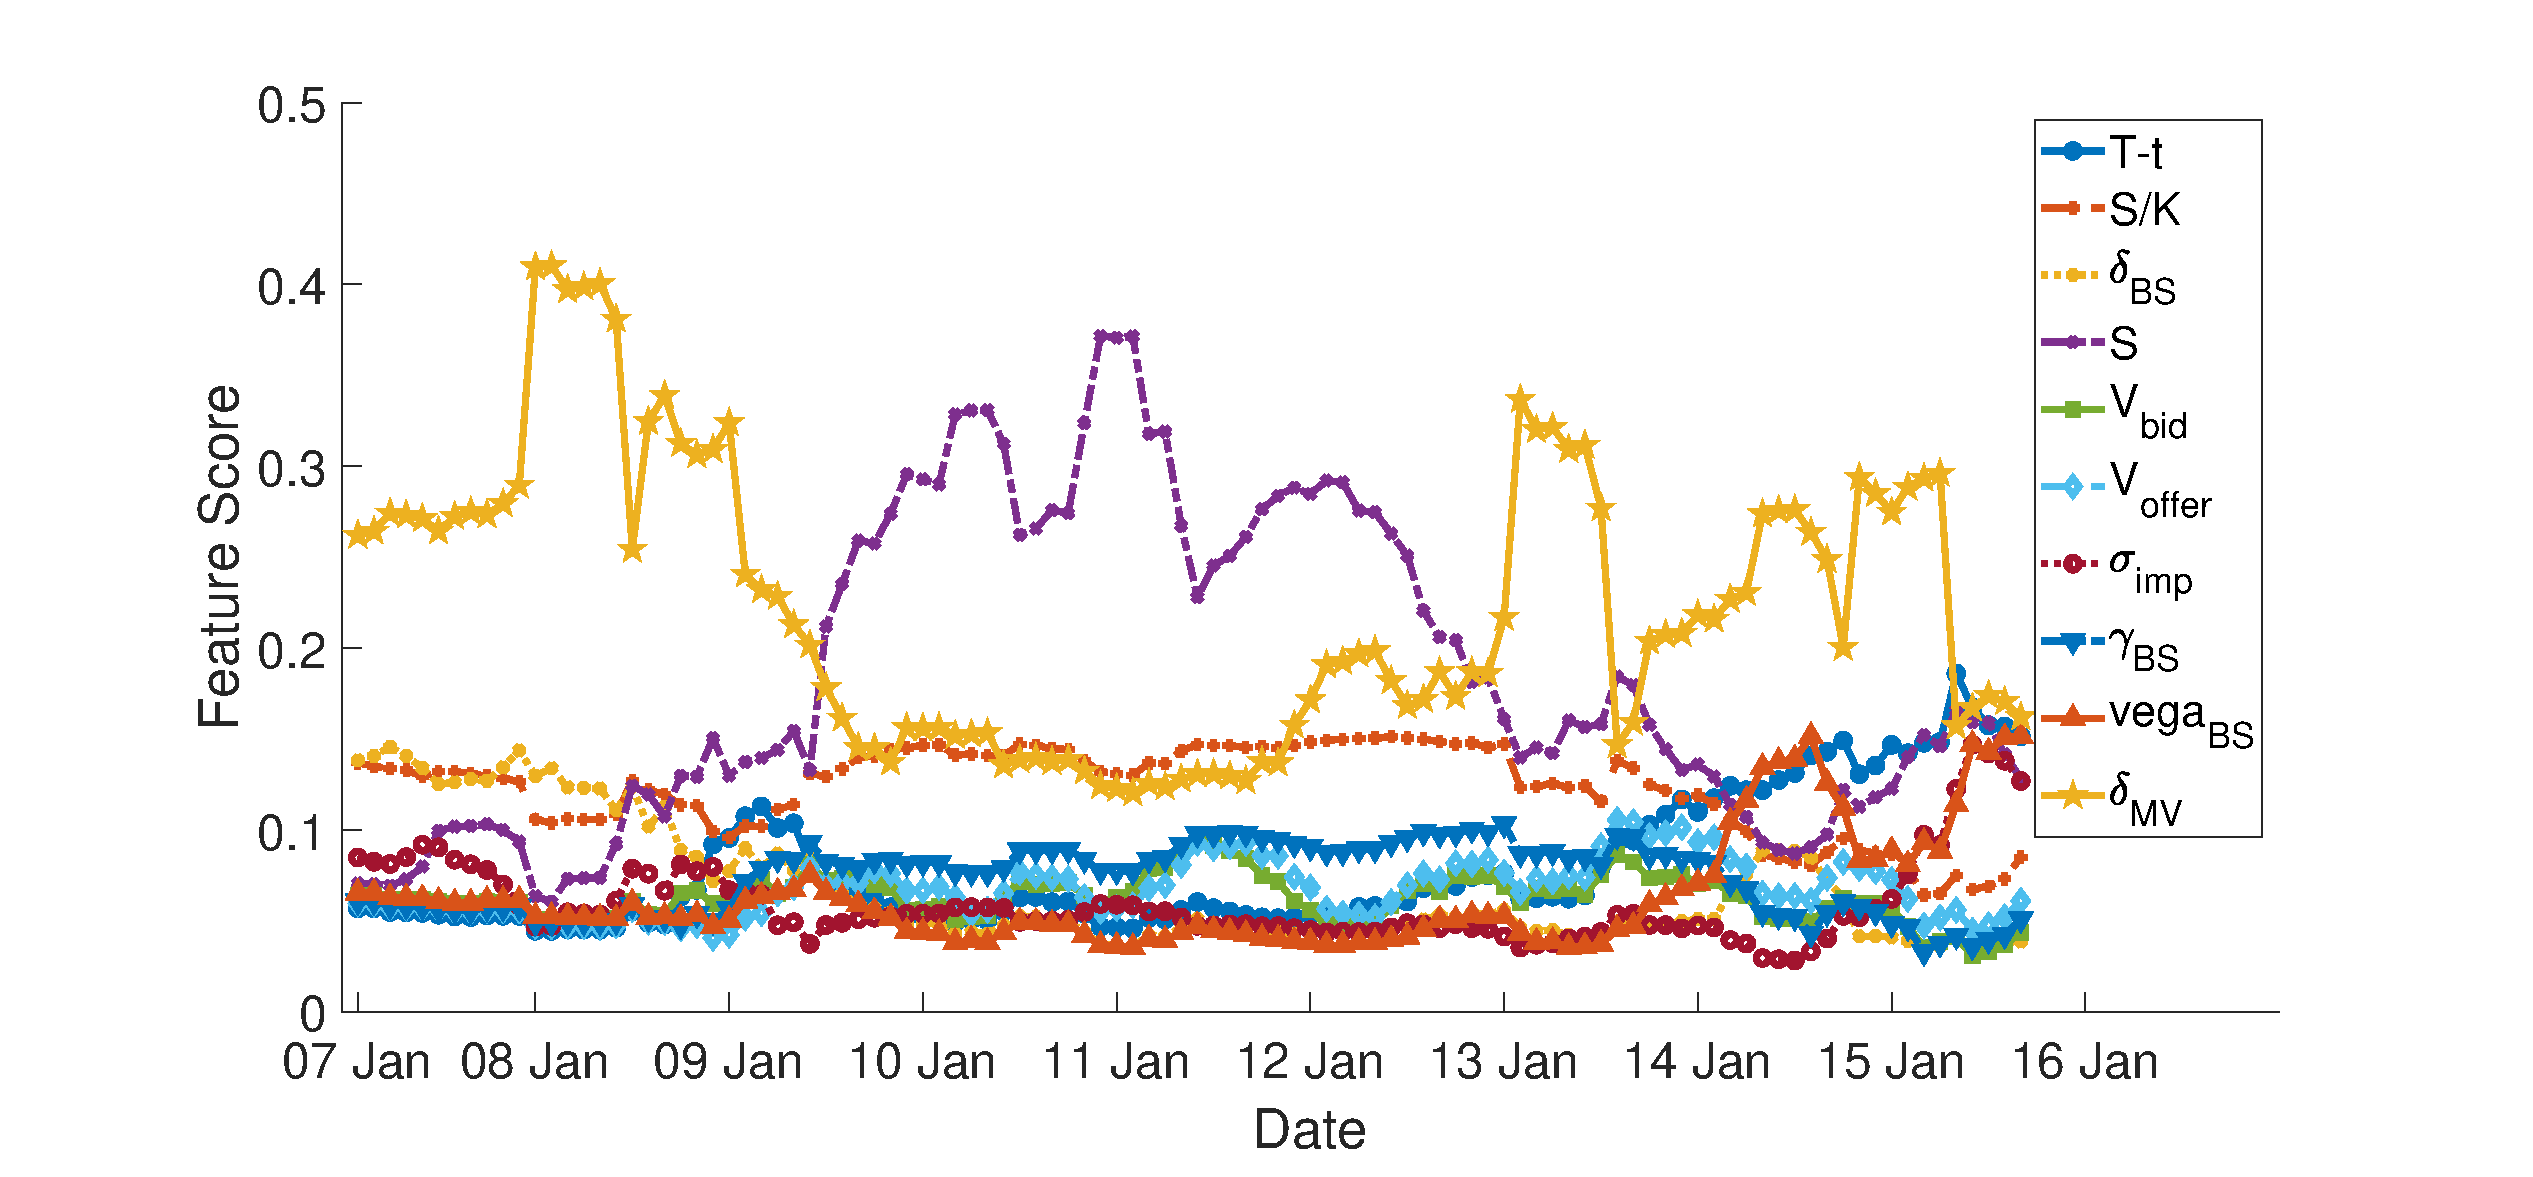
\includegraphics[width=0.48\textwidth]{./figures/CLocal0}}
\subfigure[Sequential Features Daily Hedging]{
	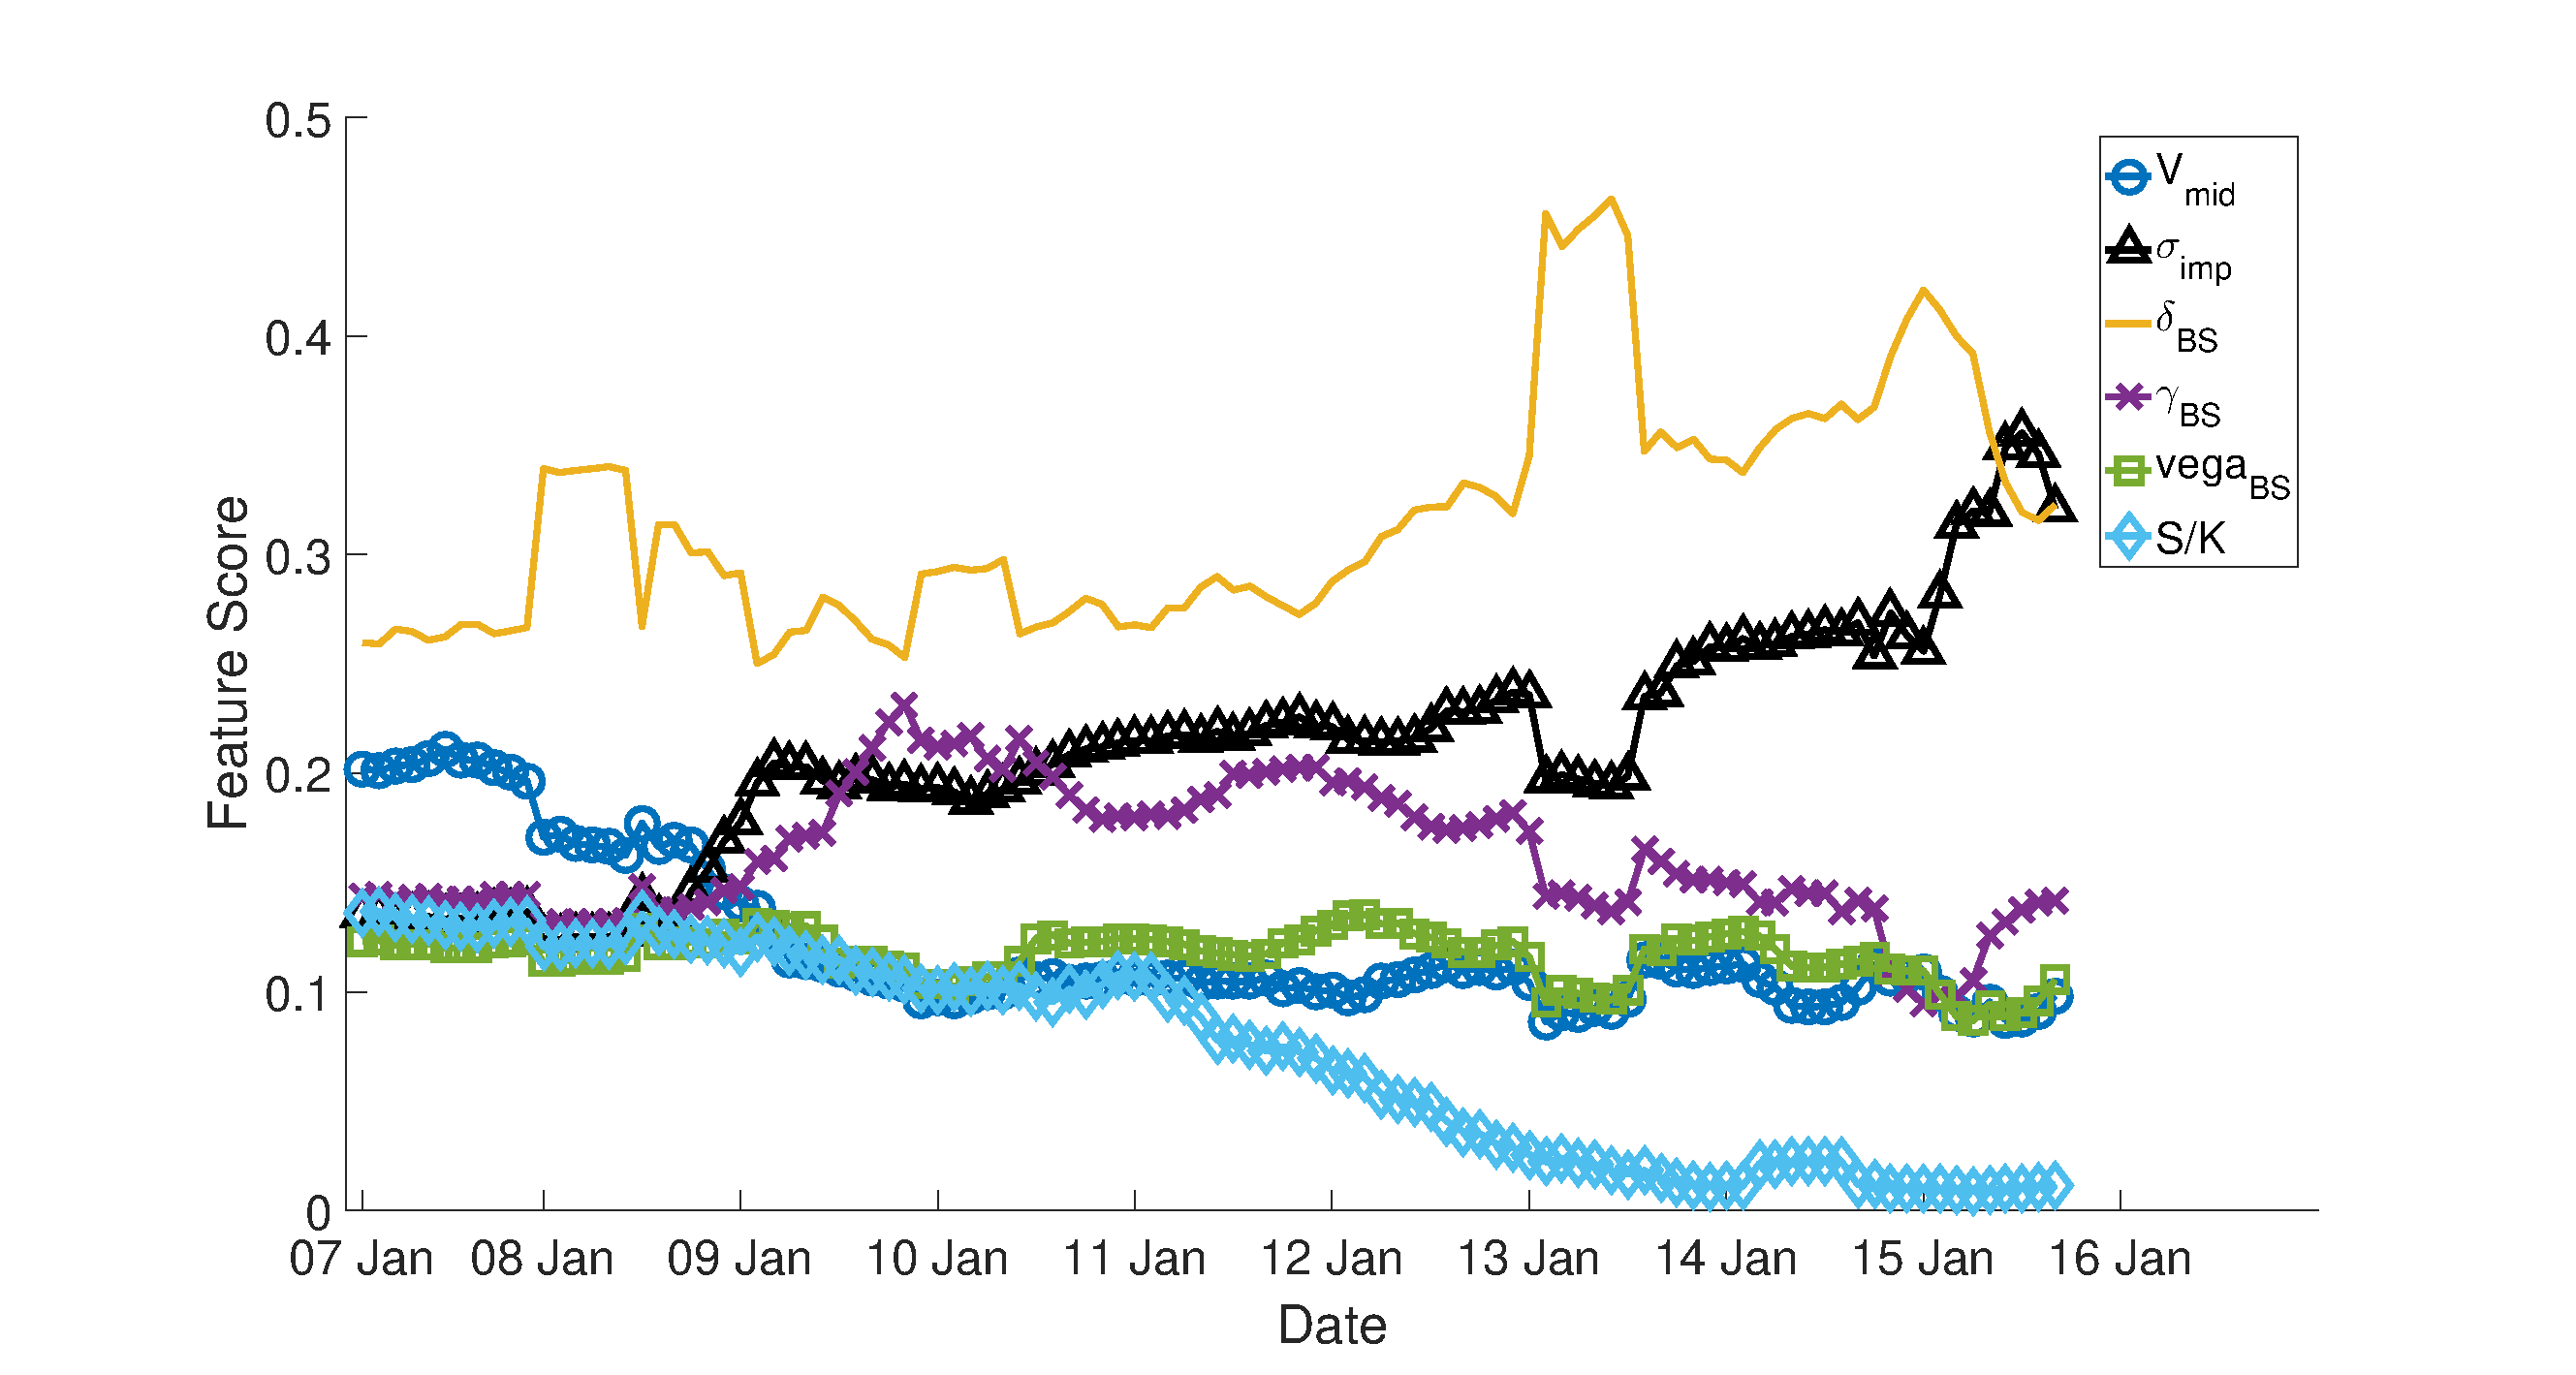
\includegraphics[width=0.48\textwidth]{./figures/C0}}
\caption{Feature score for daily hedging model $\model$: S\&P500 call option (traded data)} \label{fig:call1daily}
\end{figure}

From subplots (a) and (b) in Figure \ref{fig:put1daily}, it can be observed that the index price $S$ is often ranked as the most important local feature for daily hedging put options. The past implied volatility sequence, the past  BS delta sequence, and the past option price $V_{mid}$  are often identified as the three important sequential features.
\begin{figure}[htp]
\centering
\subfigure[Local Features Daily Hedging]{
	\includegraphics[width=0.48\textwidth]{./figures/PLocal0}}
\subfigure[Sequential Features Daily Hedging]{
	\includegraphics[width=0.48\textwidth]{./figures/P0}}
\caption{Feature score for daily hedging model $\model$:  S\&P500 put option (traded data)} \label{fig:put1daily}
\end{figure}
\section{From Local Hedging Models to Total Hedging Models}\label{sec:Localconclusion}
A natural extension  is to extend the sequential local hedging model to be a total hedging model where we rebalance multiple times until the expiries of the options. In the following chapter \ref{sec:RNNTotal}, we discuss the challenges associated with building such models and present our exploration on the data-driven total hedging model.

\chapter{Data-Driven Sequential Learning Framework for Total Hedging Risk}
\label{sec:RNNTotal}
As we have discussed in section \ref{sec:DiscreteHedgingCriteria}, in reality, one often want to hedge until the expiry of the option. Generalizing the local hedging model $\model$ to output the multiple hedging positions by minimizing a total risk objective can lead to useful risk management strategies. From the model perspective, such enhancement is achievable. Indeed, recently a deep hedging model was proposed to minimize the total option hedging risk evaluated at the option expiry  \citep{buehler2019deep}. It is shown  that using a RNN to represent the hedging position model can be a computationally efficient framework to determine the optimal hedging function when the market is incomplete, e.g., under the transaction cost \citep{buehler2019deep}.

Although minimizing the total hedging risk, which is  the hedging portfolio value at the expiry $T$, is more desirable. There are several major obstacles in obtaining enough market data to build a data-driven total hedging model due to the fact that options listed in the exchanges often have fixed expiry dates (e.g., once a month for S\&P500 index options). The deep hedging model \citep{buehler2019deep} is only built on synthetic data. Due to the lack of market data needed to build a sufficient model, applying the  deep hedging model \citep{buehler2019deep} can be challenging in real world applications.

In this chapter, we  provide a technique to deal with issue of lack of market data. In addition, an enhanced  sequential total risk hedging model $\modelT$ is introduced to minimize a discrete total risk hedging objective. We then build the total risk hedging model $\modelT$ based on the data augmentation technique we proposed and demonstrate its effectiveness  and the performance of  the  total risk hedging model $\modelT$ using real market data experiments.  





\section{Market Data Augmentation}
\label{sec:DataAugmentation}
Recall that the discrete total hedging risk \eqref{eq:TotalObjV3} is defined as the the hedging portfolio value at expiry:
\[
P_H(T,T,K)=\sum_{j=0}^{N_{rb}-1}\left\{ \left[\frac{\Smkt_{t_{j+1}}}{D(t_{j+1},T)}-\frac{\Smkt_{t_{j}}}{D(t_{j},T)}\right] \delta^M_{t_j,T,K} \right\}+\frac{\Vmkt_{t_0,T,K}}{D(t_{0},T)}-\Vmkt_{T,T,K}
\]
where
\[D(t,T)=e^{-r(T-t)}.\]
Additionally, $P_H(t,T,K)$ is the hedging portfolio value at  time $t$ with expiry date $T$ and strike $K$.

Suppose we have $M$ hedging scenarios, a data driven model can be built by minimizing total hedging loss function such as MSE:
\[
    MSE_{total}=\frac{1}{M}\sum_{i=1}^M P_H(T_i,T_i,K_i)^2
\]

Clearly, in order to build an effective data-driven total risk hedging model, one needs to gather a sufficient  number of sample  $M$.  In addition, ideally, one should also use non-overlapping underlying asset paths to generate training and testing hedging scenarios as one often observe autocorrelation in financial time series.  
However, in reality,  we have the following challenges:
\begin{enumerate}
	\item Using non-overlapping underlying asset path to  generate training and testing scenarios is not practical. For instance, assuming we are building a data-driven model for hedging 3 months until expiry, with non-overlapping underlying asset paths, 20 years of market data can provide only 80 different non-overlapping underlying asset paths, making building a data-driven model difficult.
	\item Market Option data  is limited. 
	\begin{enumerate}
		\item Options listed in an exchange only have fixed expiry dates. For example, the expiration date for the standard S\&P 500 index option is fixed at the third Friday of each month.\footnote{Starting from 2016, CBOE also introduces weekly S\&P 500 index options which expired on Monday, Wednesday and Friday of each week. The data we gathered is up to 2015-08-31, so our experiments in this thesis does not include those data.} Therefore, if we only use market available expiration dates, the number of training scenarios will  be severely limited. 
		\item In addition, the option with specific strike $K$ and expiry $T$ may not traded or quoted on every trading date during its lifetime.
		Therefore, we will have to rely on certain parametric models calibrated to market quotes to compute the necessary features (e.g., option sensitivity), which is used as the input of the data-driven model, when there are not market quotes or prices for the specific combination of $T$ and $K$ on some trading dates. 
		

	\end{enumerate}
\end{enumerate}
In order to overcome  above challenges, we propose the following remedy.  
\begin{enumerate}
	\item Overlapping underlying asset paths are allowed.
	\item A no-arbitrage  surface is calibrated on each business day to match the market quotes and prices. We will query the calibrated surface to obtain the option prices and option sensitivities when the corresponding market data is not available. 
	\item Instead of using only market available expiration dates, we assume every business day can be the expiration date of the options. The option prices and option sensitivities for these newly added expiry dates will come from querying the no-arbitrage  surface.
\end{enumerate}


Therefore, we can greatly increase the number of training scenarios, since now the hedging scenarios can have arbitrary combinations of $T$ and $K$ even if the combinations of $T$ and $K$ are not directly observed in the market. 

\subsection{No-Arbitrage Price Surface}
\label{sec:NoArb}
In this section, we describe how to calibrate an arbitrage-free price surface on each business day from the market option quotes and prices. We want to create a price surface that is \textbf{arbitrage-free}. 
% In addition, we want to be able to \textbf{extrapolate} for  in-money options and out-of-money options.
%  In the following subsection, we will discuss the steps of calibration of the arbitrage-free surface with.

\subsubsection{Arbitrage-Free Surface From SABR Model}
Following \cite{gatheral2014arbitrage}, we majorly check whether  an implied volatility surface is free of \textit{calendar arbitrage}, and \textit{butterfly arbitrage}, which we describe below. We assume we have a collection of European call option prices $\{C(T,K)\}_{T,K}$ for a range of strikes, $K$, and expiries, $T$, from which we associate its Black-Scholes implied volatility surface $\{ \sigma^{imp}(T,K)\}_{T,K}$. We also suppose that interest rates are deterministic with the expressions $D(t,T)=e^{-r(T-t)}$ for discount factors, $t$ be trading date and $T$ be the maturity date.


\begin{enumerate}
\item  \label{item:butterfly}\underline{Butterfly Arbitrage}: Given a collection of call option prices $\{C(T,K)\}_{T,K}$, using Dupire's method or equivalent approaches \cite{dupire1994pricing} one can (at least formally) find expressions for implied probability densities $\{ p(\cdot;T,S_t) \}_{T}$ such that 
\[
C(T,K) = D(t,T) \int_{(0,\infty)} (S - K)_+ p(S;T,S_t) dS.
\]
We say that the surface $\{ \sigma^{imp}(T,K) \}_{T,K}$, where $\sigma^{imp}(T,K)$ is the black-scholes implied volatility, is free of Butterfly Arbitrage if its implied probability densities $\{p(\cdot ; T,S_t)\}_{T}$ are valid densities, i.e., $p(S;T,S_t) \geq 0$ for all $S > 0$ and $\int_{0}^{\infty} p(S;T,S_t) dS = 1$. 
Additionally, the condition $p(S;T,S_t) \geq 0$ for all $S > 0$ is equivalent to require $\frac{\partial^2 C(T,K)}{\partial K^2} > 0$ for all $K > 0$ since 
\citet{breeden1978prices} show that:
\[
	\left. \frac{\partial^2 C(T,K)}{\partial K^2} \right\vert_{K=x}=D(t,T)	p(x;T,S_t)
\]


%With this definition of $w$, we may now express $p(k;T)$ as
% \[
% p(k;T) =  \frac{g(k;T)}{ 2 \pi w(k;T) } \exp{ \left( \frac{-d_{-}(k;T)^2 }{2} \right)  }
% \]
% where 
% \begin{equation}
% g(k;T_i) := \left(1 - \frac{k \partial_k w(k;T)}{2 w(k;T_i)} \right)^2 - \frac{ \left( \partial_kw(k;T_i)\right)^2}{4}\left( \frac{1}{w(k;T)} + \frac{1}{4}  \right) + \frac{\partial_{kk}w(k;T_i)}{2} 
% \label{eqn:gfun}
% \end{equation}
% and $d_{\pm}(k)$ is as in the Black-Scholes formula. To classify butterfly arbitrage based on the TV surface, there is no butterfly arbitrage when
% \begin{enumerate}
% \item 
%  $g(k) > 0$ for all $k \in \mathbb{R}$ and 
% \item  
%  $\lim_{k \to \infty}d_+(k) = -\infty$,
% \end{enumerate}
% the above listed conditions being the natural analogue of the density being non-negative and integrating to 1. 
\item \label{item:calendar} \underline{Calendar Arbitrage}:
 Given a surface $\sigma^{imp}(T,K)$, we consider the corresponding total variance (TV) surface defined by 
 \[
 w(\tau,k) = \sigma(T,K)^2 \tau
 \]
 where $\tau =T-t$ and $k$ is parameterized by log-moneyness, i.e. $k := \log(K/F(t;T))$ and $F(t;T)=S_te^{(r-q)(T-t)}\\$ is the at-the-money forward (ATMF) price for $S_t$. 
We say that the surface $\{ \sigma^{imp}(T,K) \}_{T,K}$ is free of Calendar Arbitrage 
\begin{itemize}
\item if $\frac{\partial w(\tau,k)}{\partial T} \geq 0 $ for all $k \in \mathbb{R}, T > 0$ for continuous time data
\item if $w(\tau_i,k) \leq w(\tau_{i+1},k)$ for all $k \in \mathbb{R},  T_{i} \leq T_{i+1}$ for discrete time data 
\end{itemize}

% \item \underline{Call Spread Arbitrage}: We say that the surface $\{ \sigma(K_i,T_j) \}_{K,T}$ is free of Call Arbitrage 
% \begin{itemize}
% \item if we have $-1 \leq \frac{\partial C(T,K)}{ \partial K} \leq 0$
% \end{itemize}

\end{enumerate}

Furthermore,  given a  grid of strikes: $0=K_0<K_1<\dots<K_{max}$, and a grid of expiries $t=T_0 < T_1 < \dots< T_{max} $.   The corresponding discrete criteria \cite{carr2005note} for a grid of  option prices to be free of arbitrage are set as the following: 
\begin{enumerate}
	\item  No butterfly spread arbitrage condition:
	 \begin{equation}
	C(T_{j},K_{i-1})-C(T_{j},K_{i}) > \frac{K_i-K_{i-1}}{K_{i+1}-K_{i}}
	\left( C(T_{j},K_{i})-C(T_{j},K_{i+1})  \right)
	\label{eq:DiscreteCond1}
\end{equation}
	\item  No calendar spread arbitrage:
	\begin{equation}
	C(T_{j},K_{i})\geq C(T_{j-1},K_{i})
	\label{eq:DiscreteCond2}
\end{equation}

	% \item No call spread arbitrage condition:
	% \[
	% 0 \leq \frac{C(T_{j},K_{i-1})-C(T_{j},K_{i})}{K_i-K_{i-1}} \leq 1
	% \]
\end{enumerate}



In this thesis, we will use SABR model to obtain the option price for an strike $K$ unobserved in the market when $T$ is an expiry listed in the exchange.
% On each business day $t$, we have observed option quotes for a set of market observed expiries. We denote the market available expiries as.
% \[
% \mathbf{T}^{mkt}_t=\{ T^{t}_{0}<
% T^{t}_1 < \dots< T^{t}_{max}
% \}
% \]
% We use the superscript and subscript $t$ to indicate that above expiries are the expiries on trading date $t$ for which we have some observations of market quotes and prices.


% Since in this subsection, we are discussing how to obtain a arbitrage-free surface on a fixed date $t$, for the notational simplicity, we will omit the superscript  and subscript $t$ in this subsection, 
We denote the grid of market observed expiries on a business date $t$ to be \[
\{ T_{0}<
T_1 < \dots< T_{max}
\}
\]
We set the first expiry be $t$: $T_{0}=t$. Note that for the first expiry $T_{0}=t$, the market option value at $t$ is just the option payoff at $t$ which is $\max\{S_t-K,0\}$ (call) or  $\max\{K-S_t,0\}$ (put).  For an  expiry $T_i$, let us further define 
\[K^{mkt}(T_i)=
\{
	K^{mkt}_{1},\dots,K^{mkt}_{N_K}
\}
\] to the grid of strikes $K$  where we have market observations (quotes or traded prices) for the expiry $T$

We firstly use SABR model to obtain option price for a predetermined grid of strike $0=K_0<K_1<\dots<K_{max}$.  
to be the strikes for which market option price is available for $T_i$.
Assuming $\beta=1$, we solve
\[
\min_{\alpha,\nu,\rho} \sum_{j=1}^{N_K} \left(V_{SABR}(S,t,T_i,K^{mkt}_j,r,q;\alpha,\beta,\nu,\rho)-\Vmkt(t,T_i,K^{mkt}_j)\right)^2
\]
where $V_{SABR}(S,t,T,K,r,q;\alpha,\beta,\nu,\rho)$ is option pricing function described in section \ref{sec:SABR}.  We fix $\beta=1$ in the calibration process which assumes that the distribution of $S_T$ is log-normal.  We choose to calibrate a different model for each expiry. A different set of parameters is specified for each expiry, describing an instantaneous process. The SABR models for different expiries are completely independent from each other. We choose this approach because the single implied volatility surface calibrated for all expiries and strikes is unlikely to fit the actual surface very well and calibrating a single surface is harder and more time-consuming. 

Note that we have three parameters to be calibrated so we need to observe at least 3 data points from market to successfully build a SABR model. Therefore, the number of strikes $N_K$ is expected be larger than or equal to 3. \footnote{The $\Vmkt(t,T_i,K^{mkt}_j)$ is the mid-price of market observed best bid and  best ask prices. We use market quotes in calibration and even if the trading volume is zero, we will still include them in the calibration.}

Although SABR model is computationally efficient and can match the market volatility smile well, it is not arbitrage-free. The formula \eqref{eq:SABRExpansion} is an approximation, obtained from  an asymptotic series expansion. Its accuracy degrades if the option strikes move away from the option at-the-money (ATM) strike. As a result, the implied probability density function:
\begin{equation}
	\frac{1}{D(t,T)} \left. \frac{\partial^2 C_{SABR}(T,K)}{\partial K^2} \right\vert_{K=x}=	p(x;T,S_t) 
	\label{eq:impliedDensity}
\end{equation}
where $C_{SABR}(T,K)$ is the SABR price of a call option at strike $K$ and expiry $T$, may become negative at very low or very high strikes. Therefore, we may observe butterfly spread arbitrage in SABR prices returned by the calibrated models. In addition, for each expiry, a separate set of SABR parameters is calibrated so that calender spread arbitrage can also exist. However, the existence of calendar arbitrage will be rare since the market option prices rarely contains calendar arbitrage and therefore the SABR model, which usually matches the  market option data very well rarely produces calendar arbitrag.


Given a grid of strikes $K$ for which we aim to use SABR model to produce the option prices, if we found that the grid of prices returned by the SABR model has failed the  \textbf{discrete} arbitrage conditions for butterfly arbitrage \eqref{eq:DiscreteCond1}, we will introduce some adjustments. To fix the butterfly spread  arbitrage, we implements an risk-neutral adjustment. This adjustment substitutes the implied distribution tails by those of certain log-normal distributions. The following risk adjustment is inspired by \cite{brunner2003arbitrage}. Interested reader can refer to \cite{brunner2003arbitrage} for more details. Here we just briefly discuss the process of the adjustment.

First, we introduce lower and upper strike limits, $K_{L}$ and $K_{U}$ within which the implicit probability density function (p.d.f) $p(x;T,S_t)$ from SABR model is assumed to be valid. The lower and upper strike limit can be the maximum and minimum strike $K$ for which the  discrete no butterfly spread arbitrage condition \eqref{eq:DiscreteCond1} holds. Then we assume the adjusted p.d.f is of the form:
\[
\hat{g}(x)=\left\{ \begin{array}{ll }
\lambda_{L} \;  q(x;\mu_{L},\sigma_{L}), \;&  \text{if} \; 0<x< K_{L}\\
p(x;T,S_t) , \;&  \text{if} \; \;  K_{L} \leq x \leq K_{U}\\
\lambda_{U} \;  q(x;\mu_{U},\sigma_{U}), \;& \text{if} \; x> K_{U}
\end{array} \right.
\]
where  $q(x;\mu,\sigma)$ is the p.d.f of a  log-normal distribution:
\[
	q(x;\mu,\sigma)=\frac{1}{x\sigma \sqrt{2 \pi}}
	e^{-\frac{(\ln(x)-\mu)^2}{2 \sigma^2}}.
\]
and $p(x;T,S_t)$ is the implied probability density from the calibrated SABR model. We assume that the underlying price $S_T$ is distributed according the adjusted $p.d.f$ $\hat{g}(x)$.

We require the following condition to be satisfied:
\begin{enumerate}
\item Intergrability constraint
\begin{equation}
\int_{0}^{K_{L}}	\lambda_{L}   q(x;\mu_{L},\sigma_{L}) dx+
\int_{K_{L}}^{K_{U}}	  p(x;T,S_t)  dx+
\int_{K_{U}}^{\infty}	 \lambda_{U} \;  q(x;\mu_{U},\sigma_{U}) dx=1 
\label{eq:RND1}
\end{equation}
\item Martingale  constraint
\begin{equation}
\int_{0}^{K_{L}}	 x \lambda_{L}   q(x;\mu_{L},\sigma_{L}) dx+
\int_{K_{L}}^{K_{U}}	  x p(x;T,S_t)  dx+
\int_{K_{U}}^{\infty}	 x \lambda_{U} \;  q(x;\mu_{U},\sigma_{U}) dx=F(t,T)
\label{eq:RND2}
\end{equation}
The intergrability constraint ensures that $\hat{g}(x)$ is a valid $p.d.f$. The martingale  constraint ensures thate $E[S_T]=F(t,T)$ under ther adjusted $p.d.f$.


% \item Continuity of density function constraint:
% \begin{equation}
% \lambda_{L} q(K_{L};\mu_{L},\sigma_{L})=p(K_{L};T,S_t)
% \label{eq:RND3}
% \end{equation}
% \begin{equation}
% \lambda_{U} q(K_{U};\mu_{U},\sigma_{U})=p(K_{U};T,
% S_t)
% \label{eq:RND4}
% \end{equation}
\end{enumerate}
We solve the equations \eqref{eq:RND1} and \eqref{eq:RND2} for the unknown parameters $\{\mu_{L}, \mu_{U},\sigma_{L},\sigma_{U}, \lambda_{L}, \lambda_{U}\}$.

Let:
\begin{itemize}
\item  $C_{BS}(T,K;\sigma)$ and $P_{BS}(T,K;\sigma)$ be the call and put option prices from Black-Scholes model with the Black-Scholes volatility $\sigma$.
\item  $DC_{BS}(T,K;\sigma)$ and $DP_{BS}(T,K;\sigma)$ be the digital call and put option prices from Black-Scholes model with the Black-Scholes  volatility $\sigma$  where a digital call pays one dollar if the underlying price exceeds the strike and a digital put pays the same amount  if the underlying is below the strike. 
\item  $\sigma_B$ be implied Black's volatility given by the SABR apprximation formula \eqref{eq:SABRExpansion} for $K \in [K_{L},K_{U}]$. For simplicity, we write $\sigma_{B}(K)$ to denote the implied Black's volatility given by the SABR formula \eqref{eq:SABRExpansion} for a strike $K$ and the expiry $T$.
 \end{itemize}

 Additionally, observing that the Black-Scholes \cite{black1973pricing} model implies that, under the risk neutral measurement, the prices of the underlying asset $S_T$ at the maturity $T$ are log-normal distribued:
 \[
 \ln(S_T) \sim  \mathcal{N}(\ln(S_t)+(r-q-\frac{\sigma^2}{2})(T-t),\sigma^2 (T-t))
 \]
we set $\mu_L=\ln(S_t)+(r-q-\frac{\sigma_L^2}{2})(T-t)$ and $\mu_U=\ln(S_t)+(r-q-\frac{\sigma_U^2}{2})(T-t)$ such that we have only four parameters to be solved: $\{\sigma_{L},\sigma_{U}, \lambda_{L}, \lambda_{U}\}$. Furthermore, by such setting, we will have:
\begin{equation}
\begin{split}
D(t,T)\int_{0}^{K_{L}}	\lambda_{L}   q(x;\mu_{L},\sigma_{L}) dx&=\lambda_{L} DP_{BS}(T,K_{L};\sigma_{L})\\
D(t,T)\int_{K_{U}}^{\infty}	 \lambda_{U} \;  q(x;\mu_{U},\sigma_{U}) dx&=\lambda_{U} DC_{BS}(T,K_{U};\sigma_{U})\\
D(t,T)\int_{0}^{K_{L}} (K_L-x)	\lambda_{L}   q(x;\mu_{L},\sigma_{L}) dx&=\lambda_{L} P_{BS}(T,K_{L};\sigma_{L})\\
D(t,T)\int_{K_{U}}^{\infty}	(x-K_U) \lambda_{U} \;  q(x;\mu_{U},\sigma_{U}) dx&=\lambda_{U} C_{BS}(T,K_{U};\sigma_{U})\\
\end{split}
\label{eq:SABRFix0}
\end{equation}
Following equation \eqref{eq:SABRFix0}, we observe that the two constraints \eqref{eq:RND1} and \eqref{eq:RND2} can be written as:
\begin{equation}
	\begin{split}\frac{1}{D(t,T)}=&
\lambda_{L} DP_{BS}(T,K_{L};\sigma_{L})+\\
&\frac{1}{D(t,T)}-DP_{BS}(T,K_{L};\sigma_{B}(K_L))-DC_{BS}(T,K_{U};\sigma_{B}(K_U))+\\
&\lambda_{U} DC_{BS}(T,K_{U};\sigma_{U})
\end{split}
\label{eq:RND5}
\end{equation}
\begin{equation}
	 \begin{split}
		F(t,T)=&\frac{1}{D(t,T)}\lambda_L[K_{L}DP_{BS}(T,K_{L};\sigma_{L})-P_{BS}(T,K_{L};\sigma_{L})]+\\
		&F(t,T)-\frac{1}{D(t,T)}[K_{L}DP_{BS}(T,K_{L};\sigma_{B}(K_{L}))-P_{BS}(T,K_{L};\sigma_{B}(K_{L}))]-\\
		&\frac{1}{D(t,T)}[K_{U}DC_{BS}(T,K_{U};\sigma_{B}(K_{U}))+C_{BS}(T,K_{U};\sigma_{B}(K_{U}))]+\\
		&\frac{1}{D(t,T)}\lambda_U[K_{U}DC_{BS}(T,K_{U};\sigma_{U})+C_{BS}(T,K_{U};\sigma_{U})]
		\end{split}
	\label{eq:RND6}
\end{equation}
As one can easily see, if we have:

\begin{equation}
	\begin{split}
		\lambda_L DP_{BS}(T,K_{L};\sigma_L)&=DP_{BS}(T,K_{L};\sigma_{B}(K_{L}))\\
		\lambda_U DC_{BS}(T,K_{U};\sigma_U)&=DC_{BS}(T,K_{U};\sigma_{B}(K_{U}))\\
		\lambda_L P_{BS}(T,K_{L};\sigma_L)&=P_{BS}(T,K_{L};\sigma_{B}(K_{L}))\\
		\lambda_U C_{BS}(T,K_{U};\sigma_U)&=C_{BS}(T,K_{U};\sigma_{B}(K_{U}))
	\end{split}
	\label{eq:SABRFix2}
\end{equation}
we can  show the  intergrability constraint \eqref{eq:RND5} and martingale  constraint \eqref{eq:RND6} are satisified. 






 After the calibration, we will simply using the adjusted p.d.f for option pricing:
\begin{equation}
	C_{\hat{g}(x)}(T,K)=D(t,T)\int_{-\infty}^{\infty} (x-K)_+ \hat{g}(x) dx
	\label{eq:SABRFix3}
\end{equation}
We can easily verify that \eqref{eq:SABRFix3} can be written as:
\[\small
	C_{SABR}(T,K) \leftarrow C_{\hat{g}(x)}(T,K)=\left\{ \begin{array}{ll }
		\lambda_L C_{BS}(T,K;\sigma_L)\;&  \text{if} \; 0<K< K_{L}\\

		C_{BS}(T,K;\sigma_B(K))\;&  \text{if} \; \;  K_{L} \leq K \leq K_{U}\\

		\lambda_U C_{BS}(T,K;\sigma_U) \; &  \text{if} \; \;  K> K_{U}
\end{array} \right.
\]
Lastly, we observe that $\{\sigma_{L}=\sigma_{B}(K_L),\sigma_{U}=\sigma_{B}(K_U), \lambda_{L}=1, \lambda_{U}=1\}$ solves the  system of equation  \eqref{eq:SABRFix2}. 

Notice that density function $\hat{g}(x)$ calibrated following the above risk neutral adjustment maybe discontinuous at $K_L$ and $K_U$. 
If one want to ensure the continuity of the density function,  one can solve the following system of equations for  $\{\mu_{L}, \mu_{U},\sigma_{L},\sigma_{U}, \lambda_{L}, \lambda_{U}\}$:
\begin{equation}
	\begin{split}
		D(t,T)\int_{0}^{K_{L}}	\lambda_{L}   q(x;\mu_{L},\sigma_{L}) dx&=DP(T,K_{L};\sigma_{B}(K_{L})\\
		D(t,T)\int_{K_{U}}^{\infty}	 \lambda_{U} \;  q(x;\mu_{U},\sigma_{U}) dx&=DC(T,K_{U};\sigma_{B}(K_{U})\\
		D(t,T)\int_{0}^{K_{L}} (K_L-x)	\lambda_{L}   q(x;\mu_{L},\sigma_{L}) dx&=P(T,K_{L};\sigma_{B}(K_{L})\\
		D(t,T)\int_{K_{U}}^{\infty}	(x-K_U) \lambda_{U} \;  q(x;\mu_{U},\sigma_{U}) dx&=C(T,K_{U};\sigma_{B}(K_{U})\\
\lambda_{L} q(K_{L};\mu_{L},\sigma_{L})&=p(K_{L};T,S_t)\\
\lambda_{U} q(K_{U};\mu_{U},\sigma_{U})&=p(K_{U};T,
	S_t)
	\end{split}
\end{equation}
Notice that here $\mu_{L}$ and $\mu_{U}$ are parameters to be solved as well. One can  also set the tail distirbutions as the mixture of two lognormal distributions and therefore we have  more paramters to be solved as the adjustment described in \cite{brunner2003arbitrage}. Interested reader can refer to \cite{brunner2003arbitrage} for more details. In this thesis, we  use the above  risk neutral adjustment.





For calendar arbitrage, we will shift the price by the the following procedure to remove it.
\[
shift_{t_j}=-min(min_{K}(C_{SABR}(T_j,K)-C_{SABR}(T_{j-1},K)),0).	
\]
\[
	C_{SABR}(T_j,K) \leftarrow C_{SABR}(T_j,K)+shift_{t_j}
\]
 Note the shift will be zero if no calendar arbitrage is observed between $T_{j}$ and $T_{j-1}$.

 Lastly, there is a no call-spread arbitrage condition that requires the call option value decreasing in strikes:
 \[
	C(T,K_{i+1})\leq C(T,K_{i}) \; \text{when} \; K_{i+1}>K_{i}.
\]
 We notice that no violations of this condition from the prices produced by SABR model  are observed for all the empirical results in this thesis. 
 \subsubsection{Alternative Methods to SABR Calibration}
 Given volatility surface market data as a discrete set of points $\{ \sigma^{imp}_{mkt}(T,K) \}_{T,K}$, a natural question is whether static arbitrage exists. In most cases, one must 
 \begin{enumerate}
 \item Fit a parameterization to the points $\{ \sigma^{imp}_{mkt}(T,K) \}_{T,K}$, typically by time-slice as what we did with SABR model, obtaining a parameterization $\{ \widetilde{\sigma}^{imp}(T_i,K)   \}_{T_i,K} $ for each $T_i$ separately.
 \item Compute $\{ \widetilde{w}(\tau_i,k) \}_{i=1}^N$ on a fine grid of $k$ using the expression $\widetilde{w}(\tau_i,k) := \widetilde{\sigma}^{imp}(T_i,K)^2 \tau_i$   
 \item Check for the properties listed above defining condition \ref{item:butterfly}:butterfly arbitrage and condition \ref{item:calendar}: calendar arbitrage or the corresponding discrete criteria \eqref{eq:DiscreteCond1} and \eqref{eq:DiscreteCond2} as in \cite{carr2005note}. 
 \end{enumerate}
 To obtain such mappings, one typically fits a stochastic volatility model like SABR or Heston to slices of $\{\sigma^{imp}_{mkt}(T,K)\}_{T,K}$ or considers a generalized model such as Stochastic Volatility Inspired (SVI) parameterizations.  
 
 The Stochastic Inspired Volatility model (SVI) \cite{gatheral2004parsimonious} was used internally at Merrill Lynch and publicly disclosed by Jim Gatheral in 2004.  SVI is a simple  five-parameters model.  In 2012,  the Surface SVI (SSVI) \cite{gatheral2014arbitrage} is proposed by by Gatheral and Jacquier to extend SVI model to be a whole surface model. The SSVI is parameterized in a way that a  SSVI slice at a given maturity $T$ is a SVI slice with only 3 parameters. This restriction allows to get explicit sufficient conditions for absence of arbitrage, while allowing enough flexibility for calibration. The SSVI model is recently extended by \cite{hendriks2017extended} and \cite{corbetta2019robust}. If the input market data used for calibration contains arbitrage, the calibrated surface from SSVI \cite{gatheral2014arbitrage} or its extension \cite{hendriks2017extended,corbetta2019robust} can typically be viewed as the surface that is as close as possible to the original market data, while staying arbitrage-free. In this section we briefly review a recent variant dd-eSSVI ( data-driven extended SSVI) method \cite{corbetta2019robust} as an example.
 
 
 
 
 
%  \subparagraph{Arbitrage-free parameterizations} 
 
%  As seen in \cite{gatheral2004parsimonious}, \cite{gatheral2014arbitrage}, \cite{hendriks2017extended}, \cite{corbetta2019robust}, and others, many parameterizations of implied volatility or total variance are equipped with a mode where the calibrated surface is also arbitrage-free. If the input market data used for calibration contains arbitrage, the calibrated surface can typically be viewed as the surface that is as close as possible to the original market data, while staying arbitrage-free. 
 
%  This leads us to make the distinction between the two parameterization types for given discrete market data $\{ \sigma(K_i,T_j) \}_{i,j}$ or $\{ w(k_i,T_j) \}_{i,j}$  
%  \begin{enumerate}
%  \item \underline{Raw calibration}: a parameterization is fit for each time slice $T_i$ yielding an expression $\{ \sigma(K,T_j) \}_{j}$ or $\{ w(k,T_j) \}_{j}$ aimed at fitting the raw market data as closely as possible. 
%  \item \underline{Arbitrage-free calibration}: a parameterization is fit for each time slice $T_i$ yielding an expression $\{ \sigma(K,T_j) \}_{j}$ or $\{ w(k,T_j) \}_{j}$ aimed at fitting the raw market data as closely as possible \textit{while staying arbitrage-free}. 
%  \end{enumerate}
 
 
 
 %If the parameterization of $\{ \sigma^{Mkt}(K_i,T_j) \}_{i,j}$ indicates arbitrage is present in the market data, some calibration approaches $\{ \widetilde{\sigma}(K,T_i) \}_i, \{\widetilde{w}(k,T_i)\}_{i}$ also provide an alternate mode of calibration where the resulting parameterization is \textit{arbitrage-free} as in 
 %
 %the final surface is the closest calibration to $\{\sigma(K_i,T_j)\}_{i,j}$ that is also arbitrage-free. An example of such 
 
 
 \subsubsection{dd-eSSVI Parameterization}
 \label{sss:SVI}
 
 Following the work of \cite{corbetta2019robust}, we introduce the following SSVI parameterization for a surface's Total Variance (TV), $w(\tau,k)$ as
 \begin{equation}
 w(\tau,k) = \frac{1}{2}\left(\hat{\theta}_{\tau}  + \hat{\rho}_{\tau} \hat{\psi}_{\tau} k + \sqrt{ \left(\hat{\psi}_{\tau} k + \hat{\rho}_{\tau} \hat{\theta}_{\tau} \right)^2 + \left(1 - \hat{\rho}_{\tau}^2 \right)\hat{\theta}_{\tau}^2 } \right)
 \label{eqn:w}
 \end{equation}
 In this parameterization we have that 
 \begin{itemize}
 \item $\hat{\theta}_{\tau}$ is the ATM Forward TV, read directly from the surface
 \[
 \hat{\theta}_{\tau} = w(\tau,0) = \sigma(T,K_{ATMF})^2 \cdot \tau
 \]
 where $K_{ATMF}=F(t,T)$
  \item $\hat{\rho}_{\tau}$ controls the slope of the skew 
 \item $\hat{\psi}_{\tau}$ controls the curvature. 
 \end{itemize}
 
 An important feature of this parameterizations is that it provides easy way to impose sufficient conditions on the parameters so that there is no butterfly arbitrage for a given slice, and no calendar arbitrage between two time slices. Interested reader can refer the \cite{corbetta2019robust} for the detailed conditions on those parameters. 
 
 There are many different approaches for calibrating SSVI model. For example, one can use a raw calibration appraoch to fit SSVI model to market data and then check if any arbitrage exists by check the arbitrage conditions on  the calibrated parameters.
 One can also  use an arbitrage-free calibration \cite{corbetta2019robust} by imposing the  sufficient conditions on the parameters into the calibration process. Interested reader can refer to \cite{hendriks2017extended,corbetta2019robust} for more details on how to calibrate the SSVI efficiently.
  
Since thhe major goal in this thesis is not to compare  arbitrage-free surface calibration methods, we leave the exploration of the alternative methods to calibrate the arbitrage-free surface and comparing its impact on the data-driven risk hedging model as the future work of our study. 



%  \paragraph{Introduction to calibration types and the Cross-Section Method}
 
%  In this section we outline our procedure for calibrating the dd-eSSVI model to data $\{ \sigma^{imp}(T_j,K_i) \}_{i,j}$ using  a raw calibration approach. As mentioned before, we will outline a calibration routine dd-eSSVI that is free of initial guesses and relies only on simple one-dimensional minimization.
 
%  In each case one begins by re-parameterizing the data into TV and log-moneyness, $\{ w(\tau_j,k_i) \}_{i,j}$ and also fixing a grid for minimizing over $\hat{\rho}$, denoted as $\pmb{\hat{\rho}}_N$ which divides $[-1 + 1/N,1 - 1/N]$ into $N$ equally spaced points \footnote{The choice of this interval instead of $[-1,1]$ is made to avoid certain numerical issues at the end points $-1$ and $1$ which arise later in the algorithms we present.}. 
 
 
%  \subparagraph{Raw Calibration} In the raw-calibration scheme, the dd-eSSVI is fit to market data, slice-by-slice, where the parameters from various slices are independent of each other. Given its simplicity, we describe the steps here. For each maturity $T_j$:
%  \begin{enumerate}
%  \item For each $\hat{\rho}_n \in \pmb{\hat{\rho}}_N$ we construct the objective function\footnote{This choice of relative error objective function seems to work the best in our back-tests compared to other examples include sum-of-squares or absolute error minimization.} 
%  \[
%  F_{\hat{\rho}_n}(\hat{\psi}) = \sum_{i=1}^M  \frac{  | w(\tau,k_i); \hat{\psi}, \hat{\rho}_n ) - w^{mkt}(\tau,k_i)|  }{ w^{mkt}(\tau,k_i) }
%  \]
%  \item We calculate $ \hat{\psi}_n :=  \arg\min_{\hat{\psi} \in [\hat{\psi}_l,\hat{\psi}_u]} F_{\hat{\rho}_n}(\hat{\psi}) $ using a numerical minimization scheme such as Brent search. A typical choice for $\hat{\psi}_l, \hat{\psi}_u$ are $\hat{\psi}_l = 0$, $\hat{\psi}_u = 2.5$. \label{item:psiregion} 
%  \item We set $(\hat{\rho}_{T_j}, \hat{\psi}_{T_j}) = \arg\min_{ \hat{\rho}_n,\hat{\psi}_n } \{ \  F_{\hat{\rho}_n}(\hat{\psi}_n) \  \}_{n=1}^N $
%  \end{enumerate}
 
%  \subparagraph{Detecting arbitrage} To check if a raw calibration fitting \ref{eqn:w} to market data contains arbitrage, we must check the outlined conditions for butterfly and calendar arbitrage. That is, we must show that $p(k;T)$ is a valid density and $w(k;\tau_1) \leq w(k;\tau_2)$ for all $\tau_1 \leq \tau_2$. 
 
%  Since our market data will always be taken from xTrader's databases and Exotica has a delta-cutoff scheme that ensures $p(k;T)$ is asymptotically valid, we resort to only checking that $p(k;T) > 0$ for all $k$ within a certain range. 
 
 
%  \begin{align*}
%  \partial_k w(k;t) &= \frac{1}{2}\hat{\rho}_{\tau} \hat{\psi}_{\tau} +  \frac{1}{2}\frac{ \left(\hat{\psi}_{\tau} k + \hat{\rho}_{\tau} \hat{\theta}_{\tau} \right)\hat{\psi}_{\tau}  }{ \sqrt{ \left(\hat{\psi}_{\tau} k + \hat{\rho}_{\tau} \hat{\theta}_{\tau} \right)^2 + \left(1-\hat{\rho}^2_{\tau}\right)\hat{\theta}^2_{\tau}  } } \\
%  \partial_{kk} w(k;t) &= \frac{1}{2}\frac{1}{ \sqrt{ (\hat{\psi}_{\tau} k + \hat{\rho}_{\tau} \hat{\theta}_{\tau})^2 + (1-\hat{\rho}_{\tau}^2)\hat{\theta}_{\tau}^2 }   } \left(  \hat{\psi}_{\tau}^2 - \frac{ \hat{\psi}_{\tau}^2 (\hat{\psi}_{\tau}k+ \hat{\rho}_{\tau} \hat{\theta}_{\tau})^2 }{(\hat{\psi}_{\tau} k + \hat{\rho}_{\tau} \hat{\theta}_{\tau})^2 + (1-\hat{\rho}_{\tau}^2)\hat{\theta}_{\tau}^2  }    \right) 
%  \end{align*}
 
 




 





\subsubsection{Volatility Interpolation Between Expiries}
In previous section, for each $T_i$, we calibrate a separate set of SABR parameters and we then use the calibrated SABR parameters to compute option price and the associated implied volatiliy for a predetermined grid of strikes for each $T_i$. We correct for static arbitrage if we detect any of them in the option prices we produced from the SABR models. However, after the SABR calibration, we only obtain the option values for expiries listed in the market. Our final goal is get the option values for expiries that are not available in the market. In this section, we discuss how to interpolate the volatility between different exipiries. Note that even if we use SSVI instead of SABR model, this step of volatility interpolation between expiries is still needed since SSVI model and SABR model are both calibrated to match only market available expiries.

\citet{andreasen2010volatility} have introduced an efficient and arbitrage-free volatility interpolation method based on a one step finite difference implicit Euler scheme applied to a local volatility parametrization. In this thesis, we use the volatility interpolation approach to compute option price for arbitrary expiry $T$ unobserved in market.




The volatility interpolation method is based on the Dupire's equation \cite{dupire1994pricing}.  The Dupire's equation enables us to deduce the volatility function in a local volatility
model from quoted put and call options in the market.
Under a risk-neutral measure, we assume:
	\[
	\frac{d S_t}{ S_t}= \left(r-q\right)dt +\sigma(t,S_t) dZ_t
	\]
where $r$ is the risk-free interest rate and $q$ is the dividend yield.
 Let $C(T,K)$ be the call option pricing function, Dupire's equation states:
	\[
	\frac{\partial C(T,K)}{\partial T}=\frac{1}{2} {\sigma}^2(T,K)K^2  \frac{\partial^2 C(T,K)}{ \partial K^2}-(r-q) K\frac{\partial C(T,K)}{\partial K}-qC(T,K)
	\]
Define the normalized call price in terms of discount factor $D(t,T)$ and forward price $F(t,T)$ and the normalized strike $\widehat{K}$ as:
\[
\begin{split}
D(t,T)&=e^{-r(T-t)}\\
F(t,T)&=S_te^{(r-q)(T-t)}\\
\widehat{K}&=\frac{K}{F(t,T)}\\
\widehat{C}(T,\widehat{K})&=\frac{C(T,\widehat{K} F(t,T))}{D(t,T)F(t,T)}=\frac{C(T,K)}{D(t,T)F(t,T)}
\end{split}
\]
Dupire's equation can be simplified as \cite{andreasen2010volatility}\footnote{
	 We use the call option as the example but the analysis also holds for put options. More specifically, let $P(T,K)$	be the function of put option price, the Dupire's equation for put option is:
	\[
	\frac{\partial \widehat{P}(T,\widehat{K})}{\partial T}=\frac{1}{2} \widehat{\sigma}^2(T,\widehat{K}) \widehat{K}^2  \frac{\partial^2 \widehat{P}(T,\widehat{K})}{ \partial \widehat{K}^2},\;\; \widehat{\sigma}(T,\widehat{K})={\sigma}(T,K).
	\]
}:
\[
\frac{\partial \widehat{C}(T,\widehat{K})}{\partial T}=\frac{1}{2} \widehat{\sigma}^2(T,\widehat{K}) \widehat{K}^2  \frac{\partial^2 \widehat{C}(T,\widehat{K})}{ \partial \widehat{K}^2},\;\; \widehat{\sigma}(T,\widehat{K})={\sigma}(T,K)
\]

Therefore, we can recursively solve the finite difference  discretization of the Dupire's forward equation using the fully implicit method.
Observing that $T_0=t$, on the trading date $t$, the option value expiring at $t$ is just option payoff, we have the the initial condition $\widehat{C}(T_0,\widehat{K})=max(1-\widehat{K},0)$.
Furthermore, when $K=0$, we arrive at the lower boundary condition $\widehat{C}(T,0)=1$. When $K_{max}\gg S_t$, we assume the upper boundary condition $\widehat{C}(T,\widehat{K}_{max})=0$ is true. 




Given a grid of expiries $t=T_0 < T_1 < \dots< T_{max} $ and  a grid of normalized strike: $0=\widehat{K}_0<\widehat{K}_1<\dots<\widehat{K}_{max}$, \citet{andreasen2010volatility} assume $\widehat{\sigma}(T,\widehat{K})$  to be a piecewise constant functions for a given $T_i$.
\[
	\widehat{\sigma}(T_i,\widehat{K})=\left\{ \begin{array}{ll}
		\widehat{\sigma}_{T_i,\widehat{K}_0}  , \; &\text{if} \; \widehat{K} \leq \widehat{K}_0\\
		\vdots & \vdots\\
		\widehat{\sigma}_{T_i,\widehat{K}_j}  , \; &\text{if} \; \widehat{K}_{j-1}<\widehat{K} \leq \widehat{K}_j\\
		\vdots & \vdots\\
		\widehat{\sigma}_{T_i,\widehat{K}_{max}} , \; &\text{if} \;  \widehat{K} > \widehat{K}_{max} \\
		\end{array} \right.
\]
The authors further assume:
\begin{equation}
	\left. \frac{\partial^2 \widehat{C}(T,\widehat{K})}{ \partial \widehat{K}^2}\right\vert_{\widehat{K}=0}=\left. \frac{\partial^2 \widehat{C}(T,\widehat{K})}{ \partial \widehat{K}^2}\right\vert_{\widehat{K}=\widehat{K}_{max}}=0
 \label{eq:LVFCond1}
\end{equation}
From \eqref{eq:impliedDensity} one can see the second partial derivative of call prices with regards to strike $K$ is the implied density:
\[
	\frac{1}{D(t,T)} \left. \frac{\partial^2 C(T,K)}{\partial K^2} \right\vert_{K=x}=	p(x;T,S_t) 
\]
 Therefore, the boundary conditions \eqref{eq:LVFCond1} essentially assume that the probablity density at the  low strike boundary ($K=0$) and  high strike boundary ($K=K_{Max}$) is zero, which is a reasonable assumption.

 Let us assume the gaps between the strikes in the grid of strike is fixed as a constant: $\Delta K= K_{j}-K_{j-1}$ and we let $\Delta T= T_{i+1}-T_{i}$.
The fully implicit finite difference method in matrix form is:
\begin{equation}
	\begin{bmatrix}
\widehat{C}(T_{i},\widehat{K}_0)\\
\widehat{C}(T_{i},\widehat{K}_1)\\
\widehat{C}(T_{i},\widehat{K}_2)\\
\vdots\\
\widehat{C}(T_{i},\widehat{K}_{max})
\end{bmatrix}=\mathcal{\mathbb{M}}(T_{i+1},T_{i}, \widehat{\sigma}(T_i,.))
\begin{bmatrix}
\widehat{C}(T_{i+1},\widehat{K}_0)\\
\widehat{C}(T_{i+1},\widehat{K}_1)\\
\widehat{C}(T_{i+1},\widehat{K}_2)\\
\vdots\\
\widehat{C}(T_{i+1},\widehat{K}_{max})
\end{bmatrix}
\label{eq:LVFInt}
\end{equation}
where $\mathcal{\mathbb{M}}(T_{i+1},T_{i}, \widehat{\sigma}(T_i,.))$ is a tri-diagonal matrix parametrized by  $\widehat{\sigma}(T_i,.)$,  $T_{i+1}$,and $T_{i}$.  The matrix  $\mathcal{\mathbb{M}}(T_{i+1},T_{i}, \widehat{\sigma}(T_i,.))$ is then\footnote{For a non-uniform grid of strikes, we can derive a similar form for the matrix as well}:

\begin{equation}
	\begin{bmatrix}
1&&&&&\\
-Z_1&1+2Z_1&-Z_1&&&\\
&-Z_2&1+2Z_2&-Z_2&&&\\
&&\ddots&\ddots&\ddots&&\\
&&&-Z_{Max-1}&1+2Z_{Max-1}&-Z_{Max-1}\\
&&&&&1
\end{bmatrix}
\label{eq:LVFMatrix}
\end{equation}
where $Z_j=\frac{1}{2}\frac{T_{i+1}-T_{i}}{\Delta K^2}\widehat{\sigma}(T_i,K_j)$

% Therefore, we can easily invert $\mathcal{\mathbb{M}}$ and we get:
% \begin{equation}
% 	\mathcal{\mathbb{M}}^{-1} \begin{bmatrix}
% 	\widehat{C}(T_{i},\widehat{K}_0)\\
% 	\widehat{C}(T_{i},\widehat{K}_1)\\
% 	\widehat{C}(T_{i},\widehat{K}_2)\\
% 	\vdots\\
% 	\widehat{C}(T_{i},\widehat{K}_{max})
% 	\end{bmatrix}=
% 	\begin{bmatrix}
% 	\widehat{C}(T_{i+1},\widehat{K}_0)\\
% 	\widehat{C}(T_{i+1},\widehat{K}_1)\\
% 	\widehat{C}(T_{i+1},\widehat{K}_2)\\
% 	\vdots\\
% 	\widehat{C}(T_{i+1},\widehat{K}_{max})
% 	\end{bmatrix}
% 	\label{eq:LVFInt}
% \end{equation}

Given the price vector at $T_{i}$ as the input:
\[\begin{bmatrix}
	\widehat{C}(T_{i},\widehat{K}_0)&
	\widehat{C}(T_{i},\widehat{K}_1)&
	\widehat{C}(T_{i},\widehat{K}_2)&
	\cdots&
	\widehat{C}(T_{i},\widehat{K}_{max})
\end{bmatrix}\] and the matrix $\mathcal{\mathbb{M}}(T_{i+1},T_{i}, \widehat{\sigma}(T_i,.))$ , we can compute  the price vector at $T_{i+1}$:
\[
\begin{bmatrix}
	\widehat{C}(T_{i+1},\widehat{K}_0)&
	\widehat{C}(T_{i+1},\widehat{K}_1)&
	\widehat{C}(T_{i+1},\widehat{K}_2)&
	\cdots&
	\widehat{C}(T_{i+1},\widehat{K}_{max})
	\end{bmatrix}.
\]
We want  the price vector at $T_{i+1}$ produced by the above LVF to match the price vector we computed using SABR model on $T_{i+1}$. In other words, we will try to find the $\widehat{\sigma}(T_i,.)$ by solving the following non-linear least square problem:
\begin{equation}
\inf_{\widehat{\sigma}(T_i,.)} \sum_{j}(\frac{\widehat{C}(T_{i+1},\widehat{K}_j)-\widehat{C}_{SABR}(T_{i+1},\widehat{K}_j)}{Vega_{B}(T_{i+1},\widehat{K}_j)})^2
\label{eq:LVFCal}
 \end{equation}
where we set: 
%  \[	
% 	 \begin{bmatrix}
% 	\widehat{C}(T_{i+1},\widehat{K}_0)\\
% 	\widehat{C}(T_{i+1},\widehat{K}_1)\\
% 	\widehat{C}(T_{i+1},\widehat{K}_2)\\% 	\vdots\\
% 	\widehat{C}(T_{i+1},\widehat{K}_{max})
% 	\end{bmatrix}=
%  	\mathcal{\mathbb{M}}^{-1} \begin{bmatrix}
%  	\widehat{C}_{SABR}(T_{i},\widehat{K}_0)\\
%  	\widehat{C}_{SABR}(T_{i},\widehat{K}_1)\\
%  	\widehat{C}_{SABR}(T_{i},\widehat{K}_2)\\% 	\vdots\\
%  	\widehat{C}_{SABR}(T_{i},\widehat{K}_{max})
%  	\end{bmatrix}
%  \] and  
 \[
	\widehat{C}_{SABR}(T_{i+1},\widehat{K}_j)=\frac{C_{SABR}(T_{i+1},K_j)}{D(t,T_{i+1})F(t,T_{i+1})}
\]and $Vega_{B}(T_{i+1},\widehat{K}_j)$ is the vega computed using SABR model calibrated to market quotes at $T_{i+1}$.

Note that for the intial case $T_0=t$, $\widehat{C}(T_0,\widehat{K})=max(1-\widehat{K},0)$ is given as the payoff. Given $\widehat{C}(T_0,\widehat{K})$, we firstly solve \eqref{eq:LVFCal} for the $\widehat{\sigma}(T_0,.).$ After obtaining $\widehat{\sigma}(T_0,.)$, we can then recursively solve the forward system  $\eqref{eq:LVFCal}$ to get \[
	\begin{bmatrix}
		\widehat{C}(T_i,\widehat{K}_0)\\
		\widehat{C}(T_i,\widehat{K}_1)\\
		\widehat{C}(T_1,\widehat{K}_2)\\
		\vdots\\
		\widehat{C}(T_i,\widehat{K}_{max})
		\end{bmatrix}
\] sequentially for $i=1,2,\dots$




After we solved for  $\widehat{\sigma}(T_i,.), i=0,1,\dots$, for $T \in [T_i,T_{i+1}]$, we can fill in the gaps by:
	\begin{equation}
	\begin{bmatrix}
	\widehat{C}(T,\widehat{K}_0)\\
	\widehat{C}(T,\widehat{K}_1)\\
	\widehat{C}(T,\widehat{K}_2)\\
	\vdots\\
	\widehat{C}(T,\widehat{K}_{max})
	\end{bmatrix}=\mathcal{\mathbb{M}}^{-1} (T,T_{i}, \widehat{\sigma}(T_i,.))\begin{bmatrix}
		\widehat{C}_{}(T_{i},\widehat{K}_0)\\
		\widehat{C}_{}(T_{i},\widehat{K}_1)\\
		\widehat{C}_{}(T_{i},\widehat{K}_2)\\
		\vdots\\
		\widehat{C}_{}(T_{i},\widehat{K}_{max})
		\end{bmatrix}
		\label{eq:LVFFill}
	\end{equation}
where $\mathcal{\mathbb{M}} (T,T_{i}, \widehat{\sigma}(T_i,.))$ is a tri-diagonal matrix parametrized by  $\sigma(T_i,.)$, $T$ and $T_i$. Note that $\sigma(T_i,.)$ is known after the calibration \eqref{eq:LVFCal}.
We then recover the call price by:
\[
C(T,K)=\widehat{C}(T,\widehat{K}){D(t,T)F(t,T)}
\]
Interpolation based on the above procedure can guarantee the option prices computed is arbitrage-free. Detailed proofs are as the following:
\begin{thm}
	On the discrete strike grid $\widehat{K}_0,\dots, \widehat{K}_{Max}$, 
	, the finite difference scheme \eqref{eq:LVFInt} and  \eqref{eq:LVFFill} produces option prices that are consistent with absence of arbitrage, i.e., the generated call option prices are decreasing in strikes, increasing in maturity and convex in strikes:
	\[
		C(T_i,K_{i})\leq C(T_{i},K_{i-1}) \; \text{ when } K_{i}>K_{i-1}
	\]
	\[
			C(T_i,K_{i})\geq C(T_{i-1},K_{i}) \; \text{ when } T_{i}>T_{i-1}
	\]
	\[
	C(T,K_{i-1})-C(T,K_{i}) > \frac{K_i-K_{i-1}}{K_{i+1}-K_{i}}\left( C(T,K_{i})-C(T,K_{i+1})  \right) \text{ when } K_{i+1}>K_{i}>K_{i-1}
	\]
 
\end{thm}
	
\begin{proof}
	On the discrete strike grid $\{\widehat{K}_0,\dots, \widehat{K}_{Max}\}$, the finite difference scheme \eqref{eq:LVFFill} can be written as the matrix equation system 
	\begin{equation}
		(I-\mathcal{\mathbb{S}} \mathcal{\mathbb{D}})\widehat{C}(T)=\widehat{C}(T_i),\; i=0,1,2,\dots
		\label{eq:LVFProof1}
	\end{equation}
	where $\widehat{C}(T)=\begin{bmatrix}
		\widehat{C}(T,\widehat{K}_0)&
		\widehat{C}(T,\widehat{K}_1)&
		\widehat{C}(T,\widehat{K}_2)&
		\cdots&
		\widehat{C}(T,\widehat{K}_{max})
		\end{bmatrix}$ is a vector of option prices, $I$ is the identity matrix, $\mathcal{\mathbb{S}}$ is a diagonal matrix and $\mathcal{\mathbb{D}}$ is proportional to the discrete second order difference matrix. Specifically:
		\begin{equation}
			\mathcal{\mathbb{S}}=	\begin{bmatrix}
				\widehat{\sigma}(T_i,\widehat{K}_{0}))^2&&\\
				\vdots&\ddots&\vdots\\
				&&\widehat{\sigma}(T_i,\widehat{K}_{Max})^2)
		\end{bmatrix}
		\label{eq:LVFMatrixS}
		\end{equation}
		\begin{equation}
			\mathcal{\mathbb{D}}=	(T-T_i)\begin{bmatrix}
		0&0&&&&\\
		l_1&-l_1-u_1&u_1&&&\\
		&l_2&-l_2-u_2&u_2&&&\\
		&&\ddots&\ddots&\ddots&&\\
		&&&l_{Max-1}&-l_{Max-1}-u_{Max-1}&u_{Max-1}\\
		&&&&0&0
		\end{bmatrix}
		\label{eq:LVFMatrixD}
		\end{equation}

		where 
		\[l_i=\frac{1}{\widehat{K}_{i+1}-\widehat{K}_{i-1}}\frac{1}{\widehat{K}_{i}-\widehat{K}_{i-1}}\]
		\[u_i=\frac{1}{\widehat{K}_{i+1}-\widehat{K}_{i-1}}\frac{1}{\widehat{K}_{i+1}-\widehat{K}_{i}}\]
		We can written equation \eqref{eq:LVFProof1}  as
		\begin{equation}
		[\mathcal{\mathbb{S}}^{-1}-\mathcal{\mathbb{D}}](\mathcal{\mathbb{S}}\mathcal{\mathbb{D}} \widehat{C}(T))=\mathcal{\mathbb{D}} \widehat{C}(T_i)
		\label{eq:LVFProof2}
		\end{equation}
		We assume that $\widehat{\sigma}(T_i,\widehat{K})>0$ for  all $K$, therefore we can easily see that:
		\[\mathcal{\mathbb{A}}=\mathcal{\mathbb{S}}^{-1}-\mathcal{\mathbb{D}}\]
		is an M-Matrix and thus all elements of $\mathcal{\mathbb{A}}^{-1}$ are non-negative.

		We can then easily see that 
		if elements in the vector $\mathcal{\mathbb{D}}\widehat{C}(T_i)$ are all non-negative, with all elements of $\mathcal{\mathbb{A}}^{-1}$ being non-negative, we can easily show that elements in the vector $\mathcal{\mathbb{S}}\mathcal{\mathbb{D}}\widehat{C}(T)$ are all non-negative. Thus all elements in $\mathcal{\mathbb{D}}\widehat{C}(T)$ are non-negative which is equivalent to show that:

		\[
				C(T,K_{i-1})-C(T,K_{i}) > \frac{K_i-K_{i-1}}{K_{i+1}-K_{i}}\left( C(T,K_{i})-C(T,K_{i+1})  \right).
		\]

		Notice that we start with $\widehat{C}(T_0,\widehat{K})=max(1-\widehat{K},0)$ which is the normalized payoff. Therefore, all elements in $\mathcal{\mathbb{D}}\widehat{C}(T_0)$ are non-negative. We can consequently show that all elements in $\mathcal{\mathbb{D}}C(T_i)$ are non-negative where $i=1,\dots$ since we recursively solve those optimization.  We therefore prove the convexity in strikes which proves the absence of butterfly arbitrage.

		Furthermore, differentiating \eqref{eq:LVFProof2} by $T$, we have:
		\begin{equation}
			\frac{\partial \widehat{C}(T)}{ \partial T} =\mathcal{\mathbb{A}}^{-1}  \frac{\partial \mathcal{\mathbb{D}}}{\partial T} C(T)=\frac{1}{T-T_i}\mathcal{\mathbb{A}}^{-1}  \mathcal{\mathbb{D}} \widehat{C}(T) 
			\label{eq:LVFProof3}
		\end{equation}
		Since we already prove the convexity in strikes which means elements in $\mathcal{\mathbb{D}} \widehat{C}(T)$ are all non-negative and all elements in $\mathcal{\mathbb{A}}^{-1}$ are non-negative, we can further conclude that all elements in  $\frac{\partial \widehat{C}(T)}{ \partial T}$ are non-negative. Therefore we prove the generated option prices are increasing in maturity which proved the absence of calendar arbitrage.

		Lastly, since at $T_0=t$, $\widehat{C}(T_0,\widehat{K})=max(1-\widehat{K},0)$ is the normalized payoff which is monotonically decreasing in strikes. 
		Follwing equation \eqref{eq:LVFProof3}, we have $\left.\frac{\partial \widehat{C}(T)}{ \partial T} \right|_{T=T_0}$ being monotonically decreasing in strikes. Thus,  we conclude that:
		\[
		C(T_0+d T)=	C(T_0)+\left.\frac{\partial \widehat{C}(T)}{ \partial T} \right|_{T=T_0} d T
		\]
		is monotonically decreasing in strikes as well. Following the same logic, we can conclude that the $C(T)$ will be monotonically decreasing in strikes which eliminate the existence of call-spread arbitrage.
\end{proof}


\subsection{Data Augmentation for Training Scenarios}
\label{sec:Augtrain}
Following the calibration process in section \ref{sec:NoArb}, we essentially obtain a parametrization of the option value at each trading date $t$: $\{V_{t}(T,K)\}_{T,K}$. Here $T$  can be any value that is larger than $t$ and smaller than the maximum expiry $T_{max}$ observed in market on date $t$. The $K$ can be any strike value.
As an example, in Figure \ref{fig:CaliExp}, we show the resulting price surface and implied  volatility surface for SP500 index call options  on 2012-01-04. In Figure $\ref{fig:CaliExp}$, we use $\tau=T-t$ to denote the time to maturity.
\begin{figure}[htp!]
	\centering
	\subfigure[Implied  Volatility Surface]{
		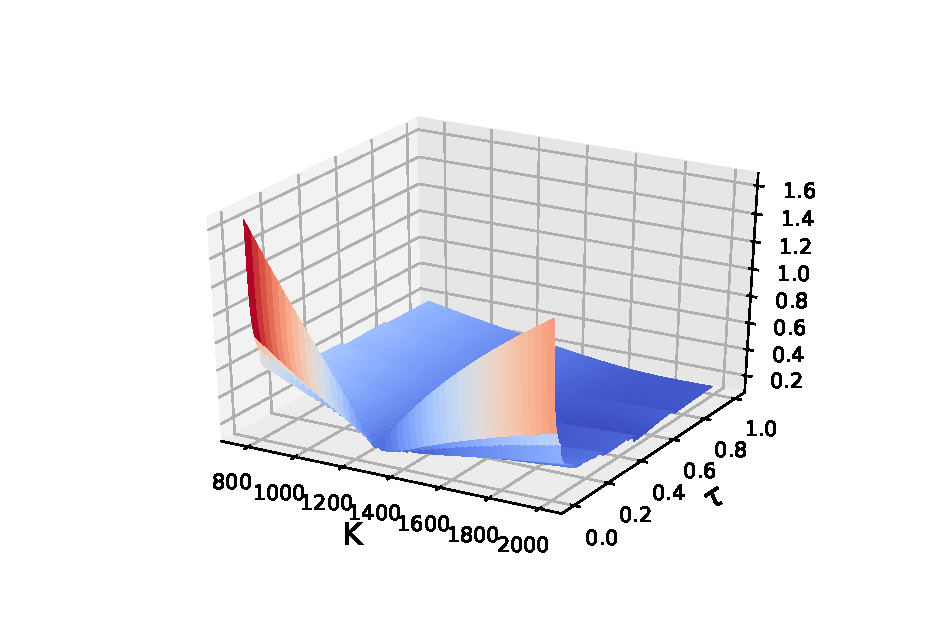
\includegraphics[width=0.8\textwidth]{./figures/ImpVol}
	}
	\subfigure[Price Surface]{
		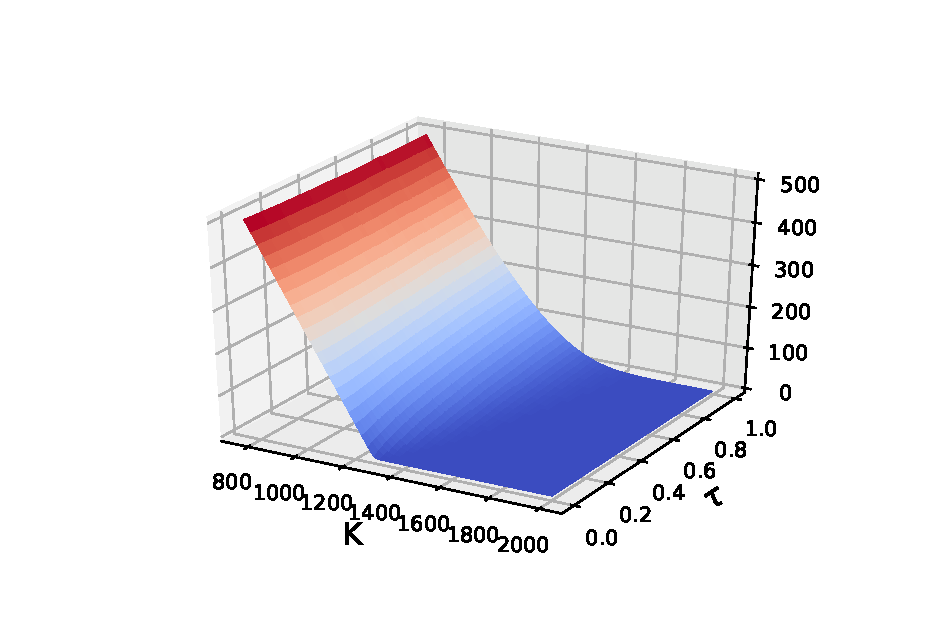
\includegraphics[width=0.8\textwidth]{./figures/Price}
	}
	\caption{The price surface and implied volatility surface calibrated for SP500 index Call Options on 2012-01-04.}
	\label{fig:CaliExp}
\end{figure}

Based on the calibration process we mentioned above, we describe the procedure of gathering the training scenarios for hedging $N_H$ business days  as the following:
\begin{enumerate}
	\item We pick a train expiry date $T$. Note that  $T$ does not have to be a real expiry that exists in market. $T$ can be any business day.
	\item We then obtain  a starting date  $t_0(T)$ to set up the hedging portfolio which is  a $N_H$-business days away from $T$. That is to say $t_0=T-N_H/250$ where we assume there are 250 business days in one year. 
	\item We check all the market observed strikes for all the business dates between $t_0$ and  $T$. Let $K^{mkt}_{max}(t_0,T)$ be the maximum of  strikes we observed in market between between $t_0$ and  $T$. 
	\item  The grid of strikes are defined as: $\mathbf{K}_{grid}(t_0,T)=\{0=K_0<K_1<\dots<2*K^{mkt}_{max}(t_0,T)\}$ where $K_i-K_{i-1}=\Delta K, i \geq 1$. In this chapter, we set $\Delta K=5$ for experiments on S\&P 500 index options which is consistent with the S\&P500 index option strike specification in real market \cite{hull2006options}.
	\item On each business day $t \in [t_0,T)$, following the calibration process in section \ref{sec:NoArb}, we  obtain a parametrization of the option value:$\{V_{t}(T,K)\}_{T,K}$. We then query $\{V_{t}(T,K)\}_{T,K}$ to obtain  option related information such as option prices and Black-Scholes sensitivities. For example, for each $K \in \mathbf{K}_{grid}(t,T)$, we extract option value by $V_{t}(T,K)$ at each business $t \in [t_0,T)$, therefore, we obtain the time series of option values from $t_0$ to $T$ for each $K$.
	\item The time series of underlying prices $S_t, t \in[t_0,T)$ are obtained directly from market. 
	% \item On each business day $t \in [t_0,T_{train})$, we can observed a set of market observed expiries: $\mathbf{T}_t^{mkt}=\{T_0^{t},T_1^{t},\dots,T_{max}^{t}\}$.
	
	
	% \item  We calibrate the SABR models for each market observed expiries $T_i^{t} \in \mathbf{T}_t^{mkt},	\;  t \in [t_0, T)$. The calibrated SABR models return the prices  for the grid $0=K_0<K_1<\dots<K_{max}$ and we fix the potential arbitrages for SABR prices returned by the SABR models, if there is any. After this process, we will have $V^{SABR}_{t,T,K}$ where $ t \in [t,T_{train}), T \in \mathbf{T}_t^{mkt}, K \in \mathbf{K}^{Aug}_{grid,T_{train}}$.
	% \item If $T_{train} \in \mathbf{T}_t^{mkt}$ and $\Vmkt_{t,T_{train},K}$ is directly observable from market. 
	% We will just use the market data to construct the time series needed for the hedging model. 
	
	% \item If $T_{train} \in \mathbf{T}_t^{mkt}$ but  the 
	% $\Vmkt_{t,T_{train},K}$ is not directly observable from market due to the fact that there is no market quote for strike $K$, we will use SABR model to fill the gaps. In this case, we assume  $\Vmkt_{t,T_{train},K}=V^{SABR}_{t,T_{train},K}$.
	
	
	% \item If $T_{train} \notin \mathbf{T}_t^{mkt}$ or we do not have enough data to calibrate a SABR model for $T_{train} \in  \mathbf{T}_t^{mkt}$, we can use the  volatility interpolation process based on LVF \cite{andreasen2010volatility} to obtain option prices on each day $t$ for the expiry $T_{train}$ we picked on step 1: $V^{LVF}_{t,T_{train},K}$ where $t \in [t_0, T_{train}), K \in \mathbf{K}^{Aug}_{grid,T_{train}}$.  In this case, we assume  $\Vmkt_{t,T_{train},K}=V^{LVF}_{t,T_{train},K}$. Furthermore, we can also obtain other option related information such as Black-Scholes delta, gamma, vega and so on.

%	
%	\item We can repeat step 1 to 7 for all $T_{train}$ within a training period. For instance, if we take 2007-01-01 to 2008-01-01 as the training period, then $T_{train}$ will be  any business day within that period.
%	\item We prepare the training data based on the augmented option data and underlying data. Please note that for the underlying asset history, we do not need to augment it since the prices of underlying asset, e.g., S\&P500 index, can be observed  on every business days.
\end{enumerate}
\subsection{Data Augmentation for Testing Scenarios}
For testing, we only test on  market observed expiries and strikes. More specifically, the procedure of gathering the testing scenarios for hedging $N_H$ business days is as the following:

\begin{enumerate}
	\item We pick a  test expiry date $T^{mkt}$. Note that  $T^{mkt}$ must be a real expiry that exists in market. We add a superscripte to emphasize that the testing expiry must be an option expiries listed in the exchanges.
	\item We then obtain  a starting date to set up the hedge portfolio $t_0$ which is  a $N_H$-business days away from $T^{mkt}$. That is to say $T^{mkt}-t_0=N_H/250$ where we assume there are 250 business days in one year. 
	\item On the starting date $t_0$, we can obtain all market option quotes for the expiry  $T^{mkt}$ and we have a grid of market strikes for expiry $T^{mkt}$ on $t_0$:
	$\mathbf{K}^{mkt}_{grid}(t_0,T^{mkt})=\{K^{mkt}_1<\dots<K^{mkt}_{N_K}\}$. Note that we have market options quotes or prices for all $K \in \mathbf{K}^{mkt}_{grid}(t_0,T^{mkt})$ on time $t_0$.
	\item On each business day $t \in [t_0,T)$, following the calibration process in section \ref{sec:NoArb}, we  obtain a parametrization of the option value:$\{V_{t}(T,K)\}_{T,K}$. 
	When there is no  market quotes $V^{mkt}(t,T^{mkt},K)$ on time $t \in [t_0, T^{mkt})$ for $K \in \mathbf{K}^{mkt}_{grid}(t_0,T^{mkt})$, we will query $\{V_{t}(T,K)\}_{T,K}$ to obtain  option related information such as option prices and Black-Scholes sensitivities. On the other hand, when  $V^{mkt}(t,T^{mkt},K)$ and associated option sensitivities  available, we use them to construct the time series needed as the input for the data-driven model.
	\item The time series of underlying prices $S_t, t \in[t_0,T)$ are obtained directly from market. 
	
	% The grid for testing is set to be $\mathbf{K}^{test}_{grid}=\{K_0=0<K_1<\dots<K_{max}\}$ where $K_i-K_{i-1}=\Delta K, i \geq 1$ and $K_{max}=2 \times K^{mkt}_{N_K}$. Please note that $\mathbf{K}^{mkt}_{t_0,T_{test}} \subset \mathbf{K}^{test}_{grid}$.  
	% \item On each business day $t \in [t,T_{test})$, we can observed a set of market observed expiries: $\mathbf{T}_t^{mkt}=\{T_0^{t},T_1^{t},\dots,T_{max}^{t}\}$.
% 	\item  We calibrate the SABR models for each market observed expires $T_i^{t} \in \mathbf{T}_t^{mkt},	\;  t \in [t_0, T),T \in \mathbf{T}_t^{mkt}$. The calibrated SABR models return the prices  for the grid of strikes and we fix the potential arbitrages for SABR prices returned by the SABR models, if there is any. 
% 	\item If $T_{test} \in \mathbf{T}_t^{mkt}, K \in \mathbf{K}^{mkt}_{t_0,T_{test}}$,  and $\Vmkt_{t,T_{test},K}$ is directly observable from market. 
% We will just use the market data to construct the time series needed for the hedging model. 
% 	\item If $T_{test} \in \mathbf{T}_t^{mkt}, K \in \mathbf{K}^{mkt}_{t_0,T_{test}}$ but  the 
% $\Vmkt_{t,T_{test},K}$ is not directly observable from market, we will use SABR model to fill the gaps. In this case,we assume  $\Vmkt_{t,T_{test},K}=V^{SABR}_{t,T_{test},K}$.
% \item
% If  we do not have enough data to calibrate a SABR model for $T_{test} \in  \mathbf{T}_t^{mkt}$, we can use the  volatility interpolation process \cite{andreasen2010volatility} to obtain option prices on each day $t$ for the expiry $T_{train}$ we picked on step 1: $V^{LVF}_{t,T_{test},K}$ where $t \in [t_0, T_{test}), K \in \mathbf{K}^{mkt}_{t_0,T_{test}}$.  In this case, we assume $\Vmkt_{t,T_{test},K}=V^{LVF}_{t,T_{test},K}$. Furthermore, we can also obtain other option related information such as Black-Scholes delta, gamma, vega and so on.
\end{enumerate}
Even if $T_{test}$ is a real expiry in market, the step 5 to 7 are frequently needed since that the options with a specific strike and expiry combination are usually not traded every day so SABR model will be needed to fill in the gaps. 
Fo ra  market observable expiry with $T-t<1$, on each date, we usually will have enough data to calibrate a SABR model. In this thesis, we are hedging for less than 1 year, so step 8 is rarely needed. For the test scenarios, we only care about real expiries  $T_{test} \in \mathbf{T}_t^{mkt}$ and real strikes $K \in \mathbf{K}^{mkt}_{t_0,T_{test}}$ in market. 





\section{Total Hedging Model}
In this section, we describe the total hedging model.
Figure \ref{fig:RNNModelTotal} depicts the proposed total discrete GRU  hedging  model $\modelT$,
which is derived from the local hedging model $\model$ we proposed in chapter \ref{sec:RNNLocal}.
This model uses the sequential features, which encode information in between two consecutive re-balancing time steps, and the hedging position from the previous re-balancing time as the input. The output hedging position is used as the input for the next re-balancing time.

Following the discrete total risk definition in section \ref{sec:DiscreteTotalRisk}, consider a hedging portfolio $P^{H}_{t,T,K}$ which is composed of:
\begin{itemize}
	\item A short position on option $\Vmkt(t,T,K)$
	\item Long $\delta^{M}_{t,T,K}$ (or short if $\delta^{M}_{t,T,K}<0$ ) shares of $\Smkt(t)$
	\item An amount in a risk-free bank account $B(t)$
\end{itemize}
For the notational simplicity, we denote:
\[
\Vmkt_{t,T,K}=\Vmkt (t,T,K)\;,\Smkt_{t}=\Smkt(t)\;,B_t=B(t)\;, P^{H}_{t,T,K}=P^{H}_{t,T,K}
\]
Also, if $\Vmkt_{t,T,K}$ is not directly observable from market, it is set to be the augmented option prices either from SABR model or LVF model as discussed in section \ref{sec:DataAugmentation}. 
Initially at $t_0$, we have
\[
P^H_{t_0,T,K}=  -V_{t_0,T,K}^{mkt}+\delta^{M}_{t_0,T,K} S_{t_0}+ B_{t_0}=0
\]
and
\[
B_{t_0}=V_{t_0}^{mkt}-\delta^{M}_{t_0,T,K} S_{t_0}
\]
Let us assume we rebalance $N_{rb}$ times until the expiry and the gap between each rebalancing time is fixed to be $\DT$:
\[
t_j=t_0+j \Delta t;\; j=0,\dots,N_{rb}-1;\;\;t_0=T-N_{rb}\DT
\]
At each rebalancing time $t_j$, we update our hedging position by changing the share we hold from $\delta^{M}_{t_{j}-\Delta t,T,K}$ to $\delta^{M}_{t_j,T,K}$ at $t_j$, where any required cash is borrowed, and any excess cash is loaned. As discussed in section \ref{sec:DiscreteTotalRisk}, the final hedging portfolio value at $T$ is:

\begin{equation}
P_H(T,T,K)=\sum_{j=0}^{N_{rb}-1}\left\{ \left[\frac{\Smkt_{t_{j+1}}}{D(t_{j+1},T)}-\frac{\Smkt_{t_{j}}}{D(t_{j},T)}\right] \delta^M_{t_j,T,K} \right\}+\frac{\Vmkt_{t_0,T,K}}{D(t_{0},T)}-\Vmkt_{T,T,K}
\label{eq:FinalHValue}
\end{equation}
where
\[D(t,T)=e^{-r(T-t)}\]
Now, consider at a arbitrary rebalancing time $t \in \{t_0,t_1, \dots, t_{N_{rb}-1}\}$, strike $K$, and expiry $T$. Assume we have computed the hedging position at previous rebalancing time $t-\Delta$: $\delta_{t-\Delta t, T,K}$. 

Let $\DT_{d}$ denote the time interval for sequential information recording. In  the subsequent empirical study, the interval $\DT_{d}$ equals one-day.  We denote the sequential features recording the daily history for hedging the option with expiry $T$ and strike $K$ as
\[
\mathbf{Y}_{t}^{T,K}=\left[\vy^{T,K}_{t-N \DT_{d}},\dots,\vy^{T,K}_{t}\right]
\]
For notational simplicity, we denote $\tau_i=t-(N+1-i)\DT_d$ with $i=1, \dots,N+1$, we thus have:
\[
\mathbf{Y}_{t}^{T,K}=\left[\vy^{T,K}_{\tau_{1}},\dots,\vy^{T,K}_{\tau_{N+1}}\right]
\]
The vector $\vy^{T,K}_{\tau_{i}} \in \Real^{d_s}$ has  $d_s$ features at time $\tau_{i}$ in the input sequential feature.
 $d_s$ is the dimension for the sequential feature $\mathbf{Y}_{t}^{T,K}$, and
$N+1$ is the length of the sequential feature sequence. We set $N=\frac{\Delta t}{\Delta t_d}$, so $\mathbf{Y}_{t}^{T,K}$ contains the sequential information in between two consecutive rebalancing time $t$ and $t-\Delta t$.
The encoder transforms information from the sequential feature $\mathbf{Y}_{t}^{T,K}$ to  a fixed-sized vector
$\mathbf{\widehat{h}}_E$   and the decoder makes the final prediction based on both $\mathbf{\widehat{h}}_E$  and the previous hedging position $\delta^{M}_{t-\Delta t,T,K}$. The overall structure of the proposed model is illustrated in Figure \ref{fig:RNNModelTotal}. 

\begin{figure}[htp!]
	\centering
	\resizebox{0.65\textwidth}{!}{
		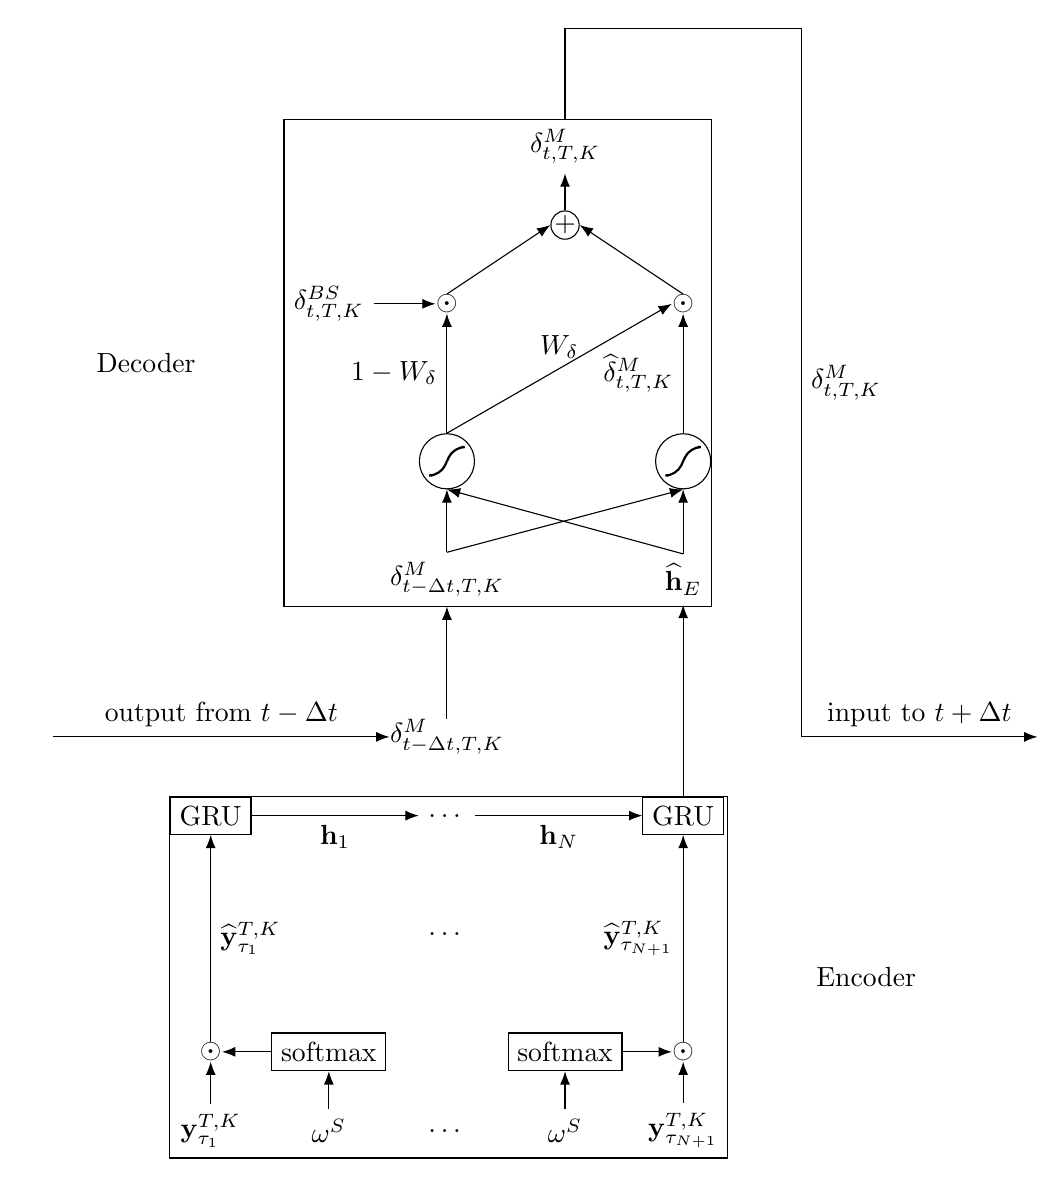
\begin{tikzpicture}[
		prod/.style={circle, draw, inner sep=0pt},
		ct/.style={circle, draw, inner sep=5pt, ultra thick, minimum width=10mm},
		ft/.style={circle, draw, minimum width=8mm, inner sep=1pt},
		filter/.style={circle, draw, minimum width=7mm, inner sep=1pt, path picture={\draw[thick, rounded corners] (path picture bounding box.center)--++(65:2mm)--++(0:1mm);
				\draw[thick, rounded corners] (path picture bounding box.center)--++(245:2mm)--++(180:1mm);}},
		mylabel/.style={font=\scriptsize\sffamily},
		>=LaTeX
		]
		
		
		\node[draw,rectangle]  (s1) at (4.5, -3) {softmax};
		\node[draw,rectangle]  (s3) at (7.5, -3) {softmax};
		\node [inner sep=0pt] (rp1) at (3*1, -3) {$\odot$};
		\node  (rp2) at (3*2, -1.5) {$\dots$};
		\node [inner sep=0pt] (rp3) at (3*3, -3) {$\odot$};
		
		\foreach \i [count=\step from 1] in {$\vy^{T,K}_{\tau_{1}}$,$\dots$,$\vy^{T,K}_{\tau_{N+1}}$}
		\node (ri\step) at (3*\step, -4) {\i};
		\node  (sw1) at (4.5, -4) {$\omega^S$ };
		\node  (sw3) at (7.5, -4) {$\omega^S$};
		\draw[->] (s1.west) to node[below]{} (rp1.east);
		\draw[->] (s3.east) to node[below]{} (rp3.west);
		\draw[->] (ri1.north) to (rp1.south);
		\draw[->] (ri3.north) to (rp3.south);
		\draw[->] (sw1.north) to (s1.south);
		\draw[->] (sw3.north) to (s3.south);
		\node (h2) at (3*2, 0.0) {$\dots$};
		\foreach \step in {1,3} {
			\node[draw,rectangle] (h\step) at (3*\step, 0.0) {GRU};
		}
		\draw[->] (rp1.north) to node[right]{$\widehat{\vy}^{T,K}_{\tau_{1}}$} (h1.south);
		\draw[->] (rp3.north) to node[left]{$\widehat{\vy}^{T,K}_{\tau_{N+1}}$} (h3.south);
		
		%\draw[->] (i4) -> (h4.south);
		\draw[->] (h1.east) to node[below]{$\vh_1$} (h2.west);
		\draw[->] (h2.east) to node[below]{$\vh_{N}$} (h3.west);
		%\foreach \step in {1,...,2} {
		%	\pgfmathtruncatemacro{\next}{add(\step,1)}
		%	\draw[->] (h\step.east) -> (h\next.west);
		%}
		\node[fit=(ri1) (ri3) (s1) (s3) (h1) (h3), draw, inner sep=0pt] (fit1) { };
		\node[align=center, outer sep=0] (encoder) [right=of fit1] {Encoder};
		
		
		
		\node[filter] (oe2) at (9, 4.5) {};
		\node[filter] (oe3) at (6, 4.5) {};
		\node [inner sep=0pt] (oe4) at (6, 6.5) {$\odot$};
		\node [inner sep=0pt] (oe5) at (9, 6.5) {$\odot$};
		\node [draw,circle,inner sep=0pt] (oe6) at (7.5, 7.5) {$+$};
		\node (oe7) at (7.5, 8.5) {$\delta^M_{t,T,K}$};
		\node  (bs) at (4.5, 6.5) {$\delta^{BS}_{t,T,K}$};
		\draw[->] (oe3.north) to node[left]{$1-W_{\delta} $} (oe4.south);
		\draw[->] (oe3.north) to node[above]{$W_{\delta}$} (oe5.west);
		\draw[->] (oe2.north) to node[left]{$\widehat{\delta}^M_{t,T,K}$} (oe5.south);
		\draw[->] (oe4.north) to node[left]{} (oe6.west);
		\draw[->] (oe5.north) to node[left]{} (oe6.east);
		\draw[->] (oe6.north) to node[left]{} (oe7.south);
		\draw[->] (bs.east) to node[left]{} (oe4.west);
		
		
		

		
		\node[inner sep=0pt]  (l1) at (6, 1) {$\delta^M_{t-\Delta t,T,K}$};
		\draw[->] (1, 1) to node[above]{output from $t-\Delta t$} (l1.west);

		
		\node (he2) at (6, 3) {$\delta^M_{t-\Delta t,T,K}$};
		\node (he3) at (9, 3) {$\widehat{\mathbf{h}}_E$};
		\draw[->] (l1.north) to (he2.south);
		\draw[->] (h3.north) to  (he3.south);
		\draw[->] (he3.north) to  (oe2.south);
		\draw[->] (he3.north) to  (oe3.south);
		
		\draw[->] (he2.north) to (oe2.south);
		\draw[->] (he2.north) to (oe3.south);
		
		\node[fit=(oe2) (oe3) (oe5) (oe6)  (oe7)  (bs) (he2) (he3), draw, inner sep=0pt] (fit3) { };
		\node[align=center, outer sep=0] (encoder) [left=of fit3] {Decoder};

		\draw (oe7.north)  to (7.5,10) to (10.5,10) to node[right]{$\delta^M_{t,T,K}$} (10.5,1);
		\draw[->] (10.5,1) to node[above]{input to $t+\Delta t$} (13.5,1);

		\end{tikzpicture}
	}
	\caption{$\modelT$: GRU encode-decoder total hedging model. The encoder summarizes the time series $\mathbf{Y}_{t}^{T,K}=\left[\vy^{T,K}_{\tau_{1}},\dots,\vy^{T,K}_{\tau_{N+1}}\right]$ as a succinct  vector $\widehat{\mathbf{h}}_E$. The decoder outputs the hedging position based on the vector $\widehat{\mathbf{h}}_E$ and the previous hedging position $\delta^M_{t-\Delta t,T,K}$ observed at the hedging time $t$. More specifically, in the decoder, a candidate output $\widehat{\delta}^M_{t,T,K}$ is firstly produced. The final output $\delta^M_{t,T,K}$ is computed based on the linear combination of BS delta $\delta^{BS}_{t,T,K}$ and the candidate output  $\widehat{\delta}^M_{t,T,K}$. The combination weight is determined by  $W_{\delta}$. The feature weight $\omega^L$ is used to compute weighted sequential feature $\widehat{\vy}^{T,K}_{\tau}$. The weighting acts as a feature selection process.
		Each edge in the graph has an arrow on it, pointing from a node whose output is used by the node pointed by the arrow as an input. The output $\delta^M_{t,T,K}$ at $t$ is used as the input for next step $t+\DT$.}
	\label{fig:RNNModelTotal}
\end{figure}
\subsection{The Difference Between  $\model$ And $\modelT$}
By comparing the $\model$ as in Figure \ref{fig:RNNModel} and the $\modelT$ as in Figure \ref{fig:RNNModelTotal}, one can notice that the model structure between $\model$ and $\modelT$ is similar to each other. Below we firstly list the differences between $\modelT$ and $\model$:
\begin{itemize}
	
	\item The most significant difference between the $\modelT$ and the $\model$ is that $\model$ is built on minimizing discrete local risk as in section \ref{sec:DiscreteLocalRisk} while $\modelT$ is built based on minimizing the discrete total risk as in in section \ref{sec:DiscreteTotalRisk}. The details of  training objective and training procedure for $\modelT$ are in later section \ref{sec:TotalModelObj} and \ref{sec:TotalModelProcedure}.
	\item In $\model$, we have a local features vector $\vx^{T,K}_{t} \in \Real^{d_l}$ which records local information at the hedging time $t$ for hedging the option with expiry $T$ and strike $K$.
	\item In $\modelT$,we no longer retain the local features vector $\vx^{T,K}_{t} \in \Real^{d_l}$ as the input to the model $\modelT$. We only retain the sequential feature  $\mathbf{Y}_{t}^{T,K}$ which contains all the sequential information between two consecutive rebalancing time $t$ and $t-\DT$. This modification is inspired by the previous total risk minimization exploration \cite{coleman2007total,schweizer1995variance}. In \cite{coleman2007total, schweizer1995variance}, the authors demonstrated the importance of using the entire path of stock instead of the current stock in determining the hedging position. Furthermore, we feel that the inclusion of $\vx^{T,K}_{t} \in \Real^{d_l}$ is a redundant design since  the sequential feature  $\mathbf{Y}_{t}^{T,K}$ contains the local information at the hedging time $t$ for hedging the option with expiry $T$ and strike $K$
	\item Since the analytical formula for the variance-optimal total risk hedging \cite{schweizer1995variance} and spline total risk minimization formulation \cite{coleman2007total} both  demonstrate the dependence of the current hedging position on the past hedging position, we include previous hedging position $\delta^{M}_{t-\Delta t,T,K}$ as the input to compute the current hedging position $\delta^{M}_{t,T,K}$. 
	
%	Additionally, we have conducted a set numerical comparisons under synthetic scenarios between $\modelT$,  the  spline total risk minimization formulation \cite{coleman2007total} and  variance-optimal total risk hedging formulation \cite{schweizer1995variance}. We demonstrate that $\modelT$ can produce equivalent hedging performance under Black-Scholes synthetic scenarios when comparing with the models in  \cite{coleman2007total} and \cite{schweizer1995variance}. More details on the comparison can be found in Appendix \ref{sec:SynCompara}.
	 
\end{itemize}
Below we briefly illustrate the model structure of $\modelT$

\subsubsection{Feature Selection via Embedded Feature Weighting}
Similarly as in $\model$, for the sequential feature $\mathbf{y}_{\tau_i}^{T,K}$,  the $j^\text{th}$ component of the normalized weight vector is given by
\[
\frac{exp(\omega^S_j)}{\sum_{i=1}^{d_s} exp(\omega^S_i)}
\]
The weighted feature vector at time  $\tau_i$ is defined as
\[
\widehat{\vy}_{\tau_i}^{T,K} =\frac{exp(\omega^S)}{\sum_{j=1}^{d_s} exp(\omega^S_j)} \odot \mathbf{y}_{\tau_i}^{T,K}
\]
\subsubsection{GRU Encoder}
At the  step $i$,  the encoder computes the value of the hidden state $\vh_{i}$ using a GRU cell. The input at the step $i$ of the encoder is $\widehat{\vy}^{T,K}_{\tau_{i}}$,  $i=1,\ldots,N+1$.
The internal structure of the GRU cell is shown in Figure \ref{fig:RNN}.

Let  $\vW_z,\vU_z,\vb_z,\vW_r,\vU_r, \vb_r,\vW_h,\vU_h,\vb_h$  denote
parameters shared by all GRU cells. We compute the $\vh_i$ as:
	\[
	\begin{split}
	\mathbf{z}_i&= sigmoid ( \vW_z \widehat{\vy}^{T,K}_{\tau_{i}} + \vU_z \vh_{i-1} +\vb_z)\\
	\mathbf{r}_i&= sigmoid ( \vW_r \widehat{\vy}^{T,K}_{\tau_{i}} + \vU_r \vh_{i-1} +\vb_r)\\
	\widehat{\vh}_i&=tanh( \vW_h \widehat{\vy}^{T,K}_{\tau_{i}}  + \vU_h (\mathbf{r}_i \odot \vh_{i-1}) +\vb_h)\\
	\vh_i&=(1-\mathbf{z}_i) \odot \vh_{i-1} + \mathbf{z}_i \odot \widehat{\vh}_i
	\end{split}
	\]
The hidden state at the last step $\vh_{N+1}$, corresponding to time ${\tau_{N+1}}={t}$, is supplied to
the decoder as the fixed size vector $\mathbf{\widehat{h}}_E$, which  extracts relevant information in $\mathbf{Y}_{t}^{T,K}$.
\subsubsection{Decoder for $\modelT$}
 The decoder of $\modelT$ computes the candidate output  $\widehat{\delta}^M_{t,T,K}$ in the following way:
\[
\widehat{\delta}^M_{t,T,K}=sigmoid (\vv^T_{out} \ tanh( \vU_{out} \mathbf{\widehat{h}}_E + \vW_{out} \delta^M_{t-\DT,T,K}+ \vb_{out})).
\]
The the output gate value $W_{\delta}$ is given by:
\[
W_{\delta}=sigmoid (\vv^T_{Gate} \ tanh( \vU_{Gate} \mathbf{\widehat{h}}_E + \vW_{Gate} \delta^M_{t-\DT,T,K}+ \vb_{Gate})).
\]
For hedging a call option, the final output from $\model$ is :
\[
\delta^M_{t,T,K}=\widehat{\delta}^M_{t,T,K} \times W_{\delta} +\delta^{BS}_{t,T,K} \times (1-W_{\delta})
\]
For hedging a put option, the final output from the model is:
\[
\delta^M_{t,T,K}=-\widehat{\delta}^M_{t,T,K} \times W_{\delta} +\delta^{BS}_{t,T,K} \times (1-W_{\delta})
\]
where $\widehat{\delta}^M_{t,T,K}$ is the candidate output.


\subsection{Training Objective For $\modelT$}
\label{sec:TotalModelObj}
Assume we have gathered hedging scenarios for a set of the unique combinations expiries $T$ and strike $K$.  
The model $\modelT$ can be built by minimizing total hedging loss function such as MSE:
\[
MSE_{total}=\sum_{(t_0,T,K)} P_H(T,T,K)^2
\]
where $P_H(T,T,K)$ is defined as in equation \eqref{eq:FinalHValue}.
A more appropriate criteria is the relative hedging error instead of the absolute total hedging error since we are mixing scenarios of different strikes together (i.e., the scenarios include near-money, in-the-money, and out-of-the money options. The absolute hedging error for in-the-money options tend to be much bigger than  near-the-money options and out-of-money options). Additionally, MSE is vulnerable to the existence of outliers. Furthermore, \citet{coleman2007total} demonstrated that the linear loss function can produce better hedging performance. Therefore, in training the $\modelT$, we use the following objective:
\begin{equation}
Obj_{total}=\sum_{(t_0,T,K)} \left|\frac{D(t_0,T)  P_H(T,T,K)}{\Vmkt_{t_0,T,K}}\right|
\label{eq:totalObjLinear}
\end{equation}
Since we notice that $\model$ is built on top of pure market data while $\modelT$ is built on top of augmented market data, we will not compare the performance of  $\model$ and $\modelT$ directly. Besides, we are curious about the effect of the choice of objective functions. Therefore, we define a new comparing model $\modelL$. The model structure of $\modelL$ is exactly the same as  $\modelT$ which is as in Figure \ref{fig:RNNModelTotal}.  The major difference is $\modelT$ is built on minimizing objective \eqref{eq:totalObjLinear}. While the $\modelL$ is built on minimizing a local risk objective.

More specifically, for a unique combination of $T$ and $K$,  at a rebalancing time $t_j$ ,we have

\[
\begin{split}
\Delta V^{mkt}_{t_j,K,T}& =D(t_0,t_{j+1}) V^{mkt}_{t_{j+1},K,T}-D(t_0,t_{j})V^{mkt}_{t_j,K,T}\\
\Delta \Smkt_{t_j} &=D(t_0,t_{j+1}) \Smkt_{t_{j+1}}-D(t_0,t_{j}) \Smkt_{t_{j}}\\
&D(t,T)=e^{-r(T-t)}\\
\end{split}
\]
\[
t_j=t_0+j \Delta t;\; j=0,\dots,N_{rb}-1;\;\;t_0=T-N_{rb}\DT
\] 
If the option price $V^{mkt}_{t,K,T}$ is not directly observable from market, we will use the augmented prices as the replacement.
The objective for the  $\modelL$  is therefore:
\begin{equation}
Obj_{Local}=\sum_{(t_j,T,K)} |\Delta V^{mkt}_{t_i,T,K}-\DS_{t_i} \delta^{M}_{t_i,T,K}|
\label{eq:LocalObjNew}
\end{equation}

\subsection{Training Procedure For $\modelT$ and $\modelL$}
\label{sec:TotalModelProcedure}
The training procedures for $\modelT$ and $\modelL$ are similar to the training procedure for $\model$. More specifically, we  initialize the  parameters using the same procedure as in section \ref{sec:init} and we pretain the $\modelT$ and $\modelL$ similarly as in section \ref{sec:preT}. Early stopping is used as the regularization techniques.We reserve the validation set to determine when to stop the training. Again the validation set is a set of the unique combinations of  expiries $T$ and strike $K$. 
We train $\modelT$ and $\modelL$ until trust region algorithms stops and select the best performing parameters based on the the total risk objective \eqref{eq:totalObjLinear} or local risk objective \eqref{eq:LocalObjNew}.
\subsubsection{Model Building Procedure}
For the experiments in the following section, We are hedging for a relatively long period (100 business days) until the expiry. Therefore, both $\modelT$ and $\modelL$ need to be updated as the market can drastically change during the hedging period. Therefore, we use the following model building procedure:
\begin{enumerate}
	\item We pick a  test expiry date $T_{test}$ and get the testing set  which is\footnote{ If we fixed the gap between two rebalancing time to be $\DT$ and we fix the number of times we rebalance the hedging portfolio to be $N_{rb}$, then given a expiry $T$, one can easily deduct the rebalance time $\{t_0,t_1, \dots, t_{N_{rb}-1}\}$ . Therefore, we can uniquely define a hedging scenario just by $T$ and $K$}:
	\[
	TestSet=\{(T,K)|,T=T_{test},K \in \mathbf{K}^{mkt}_{t_0,T_{test}}\}
	\] where $\mathbf{K}^{mkt}_{t_0,T_{test}}$ is the grid of  strikes for expiry $T_{test}$ that can be observed directly from market on the initial date $t_0$ which is 100 business away from $\modelT$.
	\item On the initial date $t_0$, we prepare the training set  and validation set to be 
		\[TrainSet=\{(T,K)|T_{min} \leq T<t_0, K \in \mathbf{K}^{Aug}_{grid,T}\}\]
			\[ValSet=\{(T,K)|T=t_0, K \in \mathbf{K}^{Aug}_{grid,T}\}\]
		where $\mathbf{K}^{Aug}_{grid,T}$ is the augmented grid of strikes for the expiry $T$ similarly defined as  in \ref{sec:Augtrain} step 4. Note that for training and validation set, we do not require $T$ and $K$ to be observed directly from market. $T_{min}$ is the earliest expiry to be included in the training set. We train the model based on the training and validation sets. We get the hedging position from either $\modelT$ or $\modelL$ for $t_0$ only: $\delta^{M}_{t_0,T,K}$ where $(T,K) \in Test_{T,K}$
		
	\item Similarly, on any rebalancing date $t_j$, we prepare the training set  and validation set to be 
	\[Train_{T,K}=\{(T,K)|T_{min} \leq T<t_j, K \in \mathbf{K}^{Aug}_{grid,T}\}\]
	\[Val_{T,K}=\{(T,K)|T=t_j, K \in \mathbf{K}^{Aug}_{grid,T}\}\]
 We retain the model from previous rebalancing date $t_{j-1}$ and we update the model based on the new training and validation sets.We get the hedging position from either $\modelT$ or $\modelL$ for $t_j$ only: $\delta^{M}_{t_j,T,K}$ where $(T,K) \in Test_{T,K}$
\end{enumerate}
Notice that in setp 3, we have included new data into the training and validation sets since the range for the allowed expiries in training set is extended from $T_{min} \leq T<t_{j-1}$ to be $T_{min} \leq T<t_{j}$.
\section{Total Discrete Hedging Performance Comparison Using  S\&P 500 index Options}
Using the S\&P 500  ({European})  index option market data from September 1, 1996 to August 31, 2015,
we  compare the total hedging performance of different hedging strategies.
We evaluate the total hedging performance using the following 5 criteria:
\begin{enumerate}
	\item The mean absolute value of the relative hedging error:
	\[
	Mean_{(t_0,T,K)}\left(\left|\frac{D(t_0,T)  P_H(T,T,K)}{\Vmkt_{t_0,T,K}}\right|\right)
	\] for all the testing scenarios.
	\item The 95\% Value-at-Risk (VaR) of the relative total hedging error $\frac{D(t_0,T) P_H(T,T,K)}{\Vmkt_{t_0,T,K}}$
	\item The 95\% Conditional-Value-at-Risk (CVaR) of the relative total hedging error $\frac{D(t_0,T) P_H(T,T,K)}{\Vmkt_{t_0,T,K}}$
	\item The 99\% Value-at-Risk (VaR) of the relative total hedging error $\frac{D(t_0,T) P_H(T,T,K)}{\Vmkt_{t_0,T,K}}$
	\item The 99\% Conditional-Value-at-Risk (CVaR) of the relative total hedging error $\frac{D(t_0,T) P_H(T,T,K)}{\Vmkt_{t_0,T,K}}$
\end{enumerate}

We test on the real expiries and real strikes in market. We build the models following the model building procedure as in section \ref{sec:TotalModelProcedure}.  The combined testing set is defined as:
\[
AllTestSet=\{(T,K)|\text{2000-01-01}\leq T \leq \text{2015-08-31},K \in \mathbf{K}^{mkt}_{t_0,T}, T \text{ is a market observed expiry}\}
\]
Namely, we test on all the market observed combinations of $(T,K)$ where the expiry $T$ is between 2000-0-01 to 2015-08-31. Note that, we have included two crisis periods: the burst of dot-com bubble  period (2000 to 2002)and subprime mortgage crisis period (2007 to 2008).
\subsection{Data and Experimental Setting}
The sequential inputs to $\modelT$ and $\modelL$, $\mathbf{Y}_{t}^{T,K}$, at a rebalancing time $t$, at each hedging time $t$, are the historical time series recorded daily from previous rebalancing time $t-\DT$ to current rebalancing time $t$ for the following features:


\begin{table}[htp!]
	\centering
	\begin{tabular}{|l|}
		\hline
		Option middle price\\ \hline
		Black–Scholes implied volatility\\
		\hline
		Black–Scholes delta\\
		\hline
		Black–Scholes vega \\
		\hline
		Bartlett delta \\
		\hline
		Time to expiry \\\hline
		S\&P500 index price\\\hline
		VIX index price\\\hline
		The moneyness $S/K$\\\hline
		Minimum variance delta $\delta_{MV}$  \eqref{eq:HullWhite}\\\hline
		Strike $K$ \\   \hline
	\end{tabular}
	\caption{Sequential features for $\modelT$ and $\modelL$ at time $t$ are the historical time series of features listed in this table.}
\end{table}

The number of hidden states, for the single-layer GRU encoder, the neural network outputting $\widehat{\delta}^M_{t,T,K}$, and the neural network outputting $W_{\delta}$  in Figure \ref{fig:RNNModelTotal}, are all set to be 5.  Specifically, we compare with the following methods,
\begin{itemize}
	\item $\modelT$: the model shown in Figure \ref{fig:RNNModelTotal} which is trained with the total risk objective \eqref{eq:totalObjLinear}.
	\item $\modelL$: the model shown in Figure \ref{fig:RNNModelTotal} which is trained with the local risk objective \eqref{eq:LocalObjNew},
	\item Bartlett: Barlett corrective  delta based on \eqref{eq:bartlett},
	\item BS: Black–Scholes delta based on the implied volatility 
\end{itemize}
The hedging period is fixed to be 100 business days. We have two different hedging frequencies: weekly and monthly hedging. For weekly hedging, we rebalance every 5 business days so the number of rebalacing times is $N_{rb}=20$. For monthly hedging, we rebalance every 20 business days so the number of rebalacing times is $N_{rb}=5$.

 
\subsection{Call Option Total Hedging Comparison}
In this subsection, we present the results for call options. We show the hedging performance for Near-The-Money(NTM), In-The-Money(ITM), Out-of-The-Money(OTM) separately.  The NTM, OTM, and ITM scanerios are classified based on the Black-Scholes delta at the initial date $t_0$ where we set up the hedging portfolio: $\delta^{BS}_{t_0,T,K}$. For call option, the criteria is:
\begin{itemize}
	\item  Near-The-Money(NTM): $0.3 \leq \delta^{BS}_{t_0,T,K} <0.7$
	\item  In-The-Money(ITM): $0.7 \leq \delta^{BS}_{t_0,T,K} <0.95$
	\item  Out-of-The-Money(OTM):  $0.05 \leq \delta^{BS}_{t_0,T,K} <0.3$
\end{itemize}
We omit the testing scenarios for deep in-the-money and deep out-of-the money options due to the fact that they are highly illiquid in market and their market quotes are highly unreliable. Also, the deep in-the-money and deep out-of-the money options are deleted from training set and validation set.
\begin{itemize}
	\item  Deep In-The-Money(ITM): $0.95 \leq \delta^{BS}_{t_0,T,K} <1.0$
	\item  Deep Out-of-The-Money(OTM):  $0.0 \leq \delta^{BS}_{t_0,T,K} <0.05$
\end{itemize}

\subsubsection{Call Option Weekly Hedging Comparison}
In Table \ref{table:CallTotalW}, we demonstrate the results on weekly hedging call options. Furthermore, in Figure \ref{fig:CallTotalW1}, Figure \ref{fig:CallTotalW2}, and  Figure \ref{fig:CallTotalW3}, we compare the distribution of the relative hedging error of $\modelT$ with the distributions of the relative hedging error of $\modelL$, BS model, and Bartlett model respectively.
\begin{table}[htp!]
	\centering
	\begin{tabular}{ll|l|l|l|}
		\cline{3-5}
		&          & Near-The-Money   & In-The-Money     & Out-of-The-Money \\ \hline
		\multicolumn{1}{|l|}{\multirow{4}{*}{Mean Abs Error}} & $\modelT$    & \textbf{0.1927}  & 0.0571  & \textbf{0.7344}  \\  
		\multicolumn{1}{|l|}{}                                & $\modelL$    & 0.2250           & 0.0866           & 0.8285           \\  
		\multicolumn{1}{|l|}{}                                & Bartlett & 0.2347           & 0.0641           & 0.7383           \\  
		\multicolumn{1}{|l|}{}                                & BS       & 0.2198           &\textbf{0.0531}           & 0.9706           \\ \hline
		\multicolumn{1}{|l|}{\multirow{4}{*}{VaR (95\%)}}     & $\modelT$    & \textbf{-0.2827} & \textbf{-0.1121} & \textbf{-0.5298} \\  
		\multicolumn{1}{|l|}{}                                & $\modelL$    & -0.3622          & -0.1806          & -0.5753          \\  
		\multicolumn{1}{|l|}{}                                & Bartlett & -0.4836          & -0.1656          & -0.9841          \\  
		\multicolumn{1}{|l|}{}                                & BS       & -0.4823          & -0.1523          & -0.8603          \\ \hline
		\multicolumn{1}{|l|}{\multirow{4}{*}{CVaR (95\%)}}    & $\modelT$    & \textbf{-0.4721} & \textbf{-0.1865} & \textbf{-1.0003} \\  
		\multicolumn{1}{|l|}{}                                & $\modelL$    & -0.5643          & -0.2081          & -1.1673          \\  
		\multicolumn{1}{|l|}{}                                & Bartlett & -0.7103          & -0.2192          & -1.4232          \\  
		\multicolumn{1}{|l|}{}                                & BS       & -0.7009          & -0.2724          & -1.2299          \\ \hline
		\multicolumn{1}{|l|}{\multirow{4}{*}{VaR (99\%)}}     & $\modelT$    & \textbf{-0.5301} & \textbf{-0.1976} & -1.5077          \\  
		\multicolumn{1}{|l|}{}                                & $\modelL$    & -0.6361          & -0.2168          & -1.3583          \\  
		\multicolumn{1}{|l|}{}                                & Bartlett & -0.778           & -0.2654          & -1.6152          \\  
		\multicolumn{1}{|l|}{}                                & BS       & -0.7171          & -0.3653          & \textbf{-1.3363} \\ \hline
		\multicolumn{1}{|l|}{\multirow{4}{*}{CVaR (99\%)}}    & $\modelT$    & -0.8205          & -0.3261 & -1.6090          \\  
		\multicolumn{1}{|l|}{}                                & $\modelL$    & \textbf{-0.7942} & \textbf{-0.2301}          & -2.1206          \\  
		\multicolumn{1}{|l|}{}                                & Bartlett & -1.0827          & -0.2883          & -2.1225          \\  
		\multicolumn{1}{|l|}{}                                & BS       & -1.0040          & -0.4712          & \textbf{-1.6074} \\ \hline
	\end{tabular}
	\caption{Summary of weekly hedging S\&P 500 call options for 100 business days with total hedging evaluation criteria. Please note that the total hedging evaluation in this table assumes we are at the sell-side of the option trading.} \label{table:CallTotalW}
\end{table}
\begin{figure}[htp!]
	\centering
	\subfigure[]{
		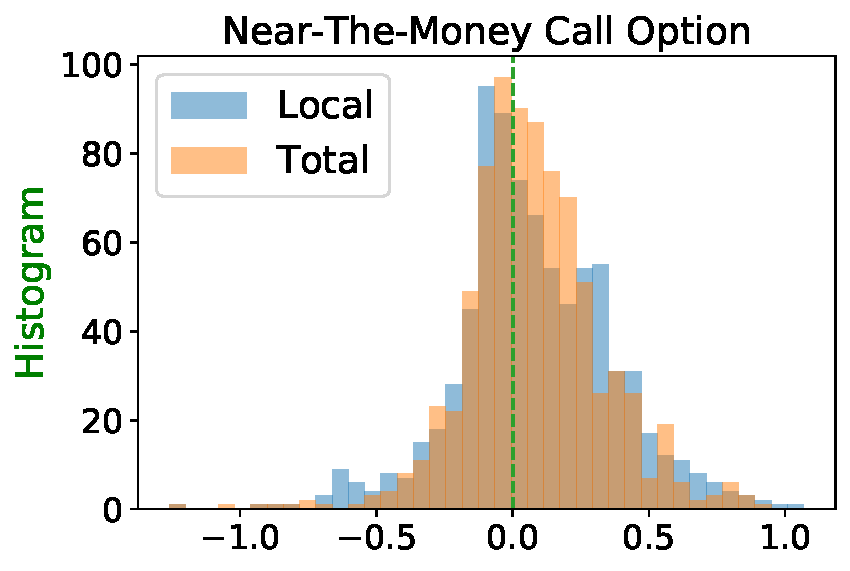
\includegraphics[width=0.32\textwidth]{./figures/WLocalVersusTotalCallNTM.pdf}}
	\subfigure[]{
		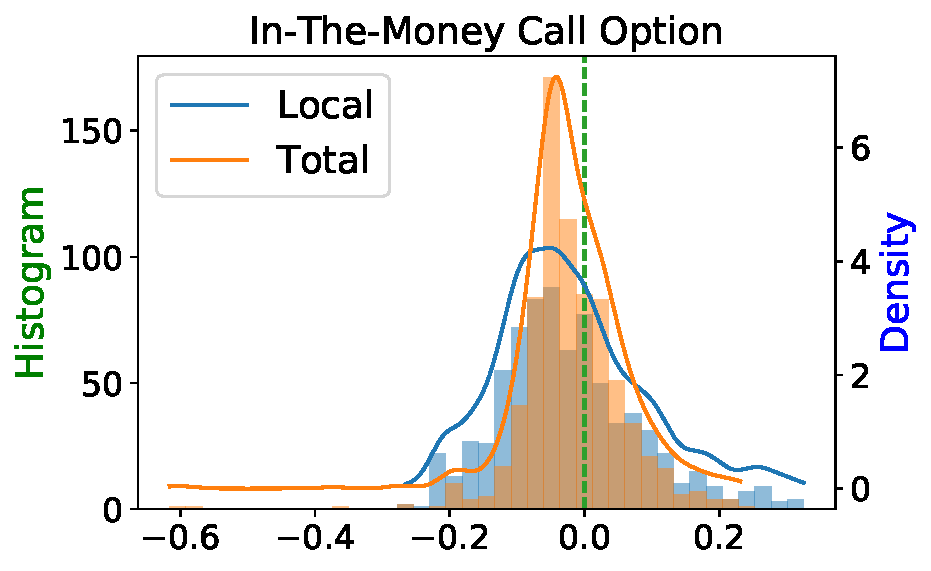
\includegraphics[width=0.32\textwidth]{./figures/WLocalVersusTotalCallITM.pdf}}
	\subfigure[]{
		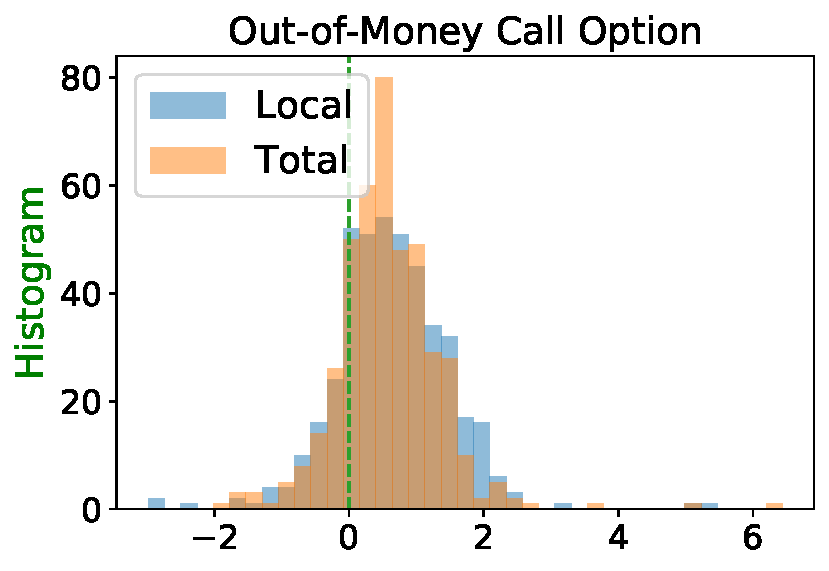
\includegraphics[width=0.32\textwidth]{./figures/WLocalVersusTotalCallOTM.pdf}}
	\caption{Comparing total model $\modelT$ and local model $\modelL$ on weekly hedging S\&P 500 call options in terms of the distribution of the  relative hedging portfolio value at the expiries Please note that the distribution in this figure assumes we are at the sell-side of the option trading.} \label{fig:CallTotalW1}
	\centering
	\subfigure[]{
		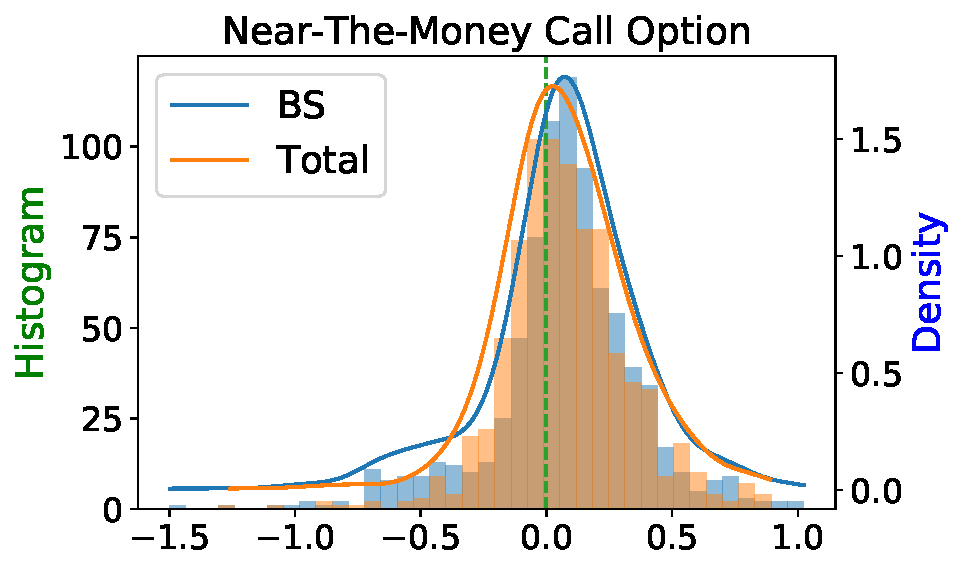
\includegraphics[width=0.32\textwidth]{./figures/WBSVersusTotalCallNTM.pdf}}
	\subfigure[]{
		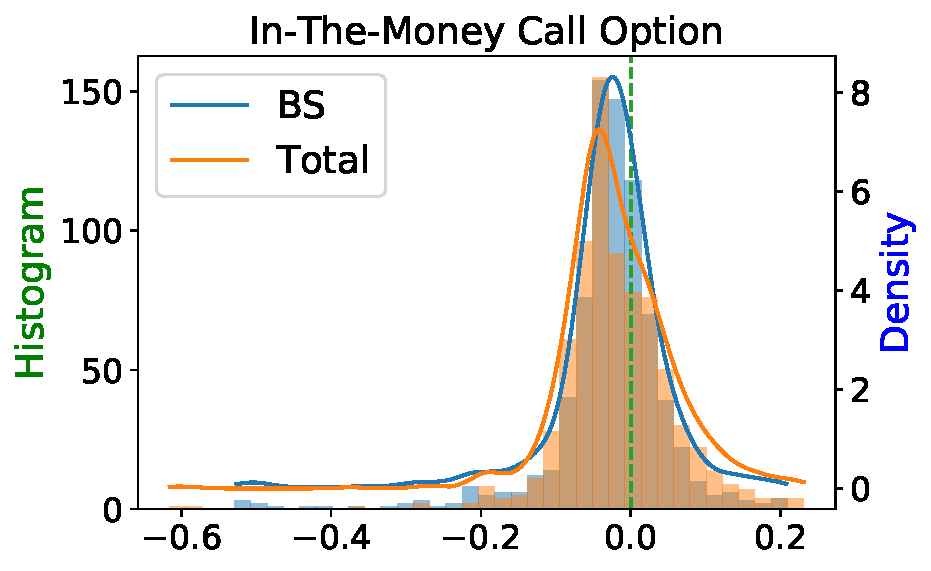
\includegraphics[width=0.32\textwidth]{./figures/WBSVersusTotalCallITM.pdf}}
	\subfigure[]{
		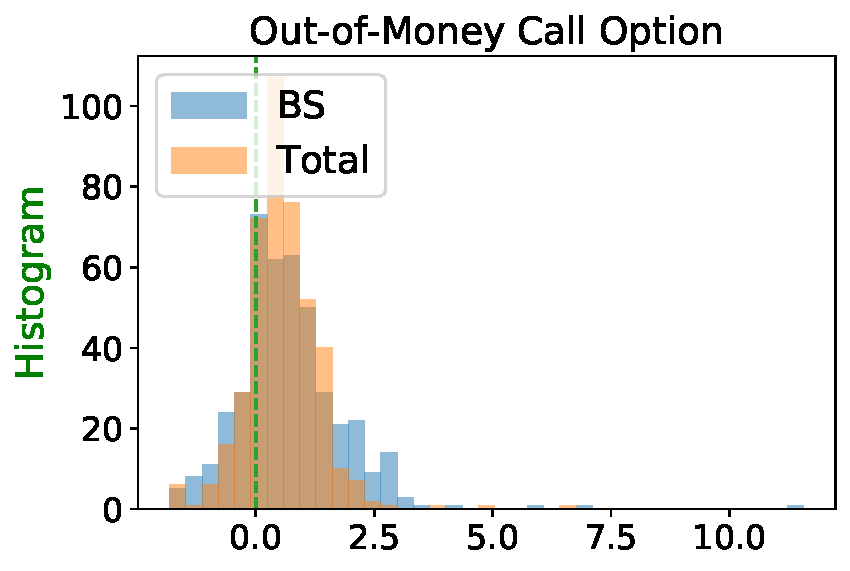
\includegraphics[width=0.32\textwidth]{./figures/WBSVersusTotalCallOTM.pdf}}
	\caption{Comparing total model $\modelT$ and BS Model  on weekly hedging S\&P 500 call options in terms of the the distribution of the  relative hedging portfolio value at the expiries. Please note that the distribution in this figure assumes we are at the sell-side of the option trading.} 
	\label{fig:CallTotalW2}
	\centering
	\subfigure[]{
		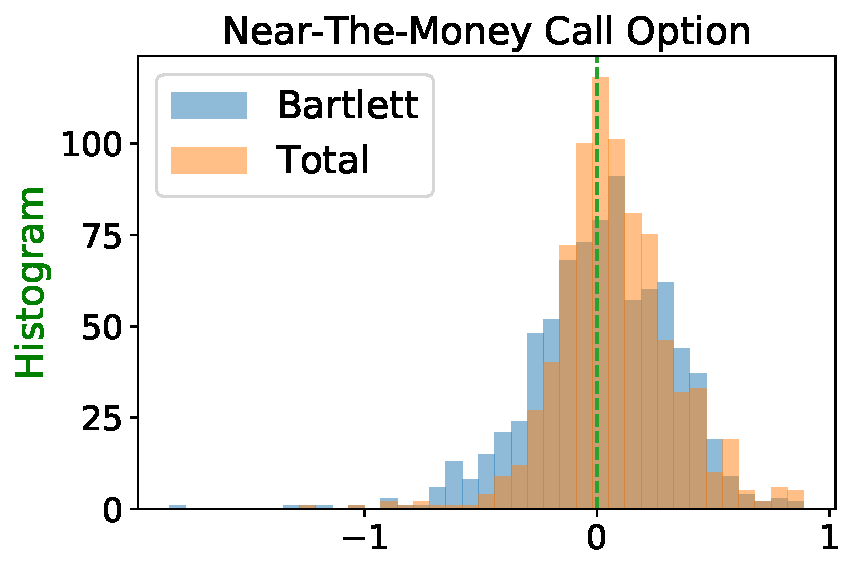
\includegraphics[width=0.32\textwidth]{./figures/WBartlettVersusTotalCallNTM.pdf}}
	\subfigure[]{
		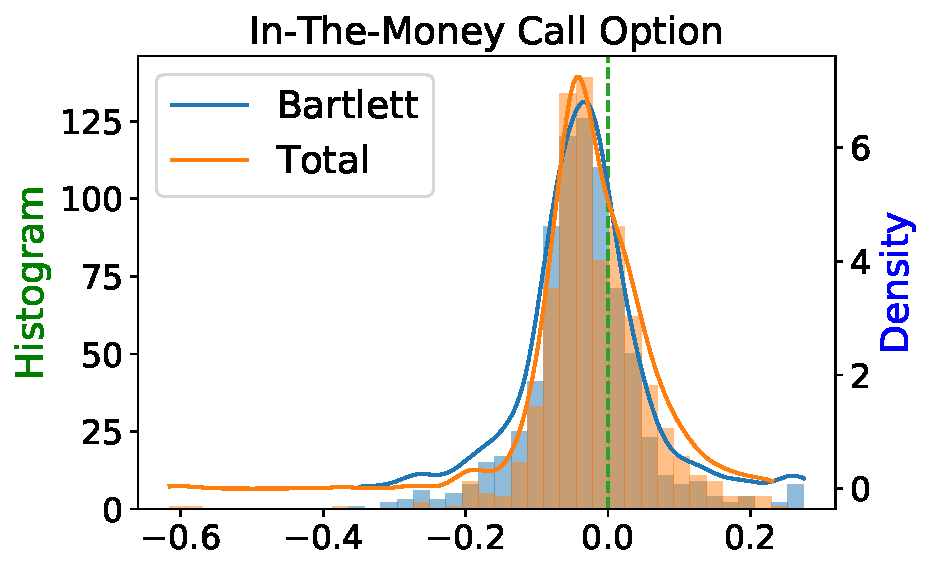
\includegraphics[width=0.32\textwidth]{./figures/WBartlettVersusTotalCallITM.pdf}}
	\subfigure[]{
		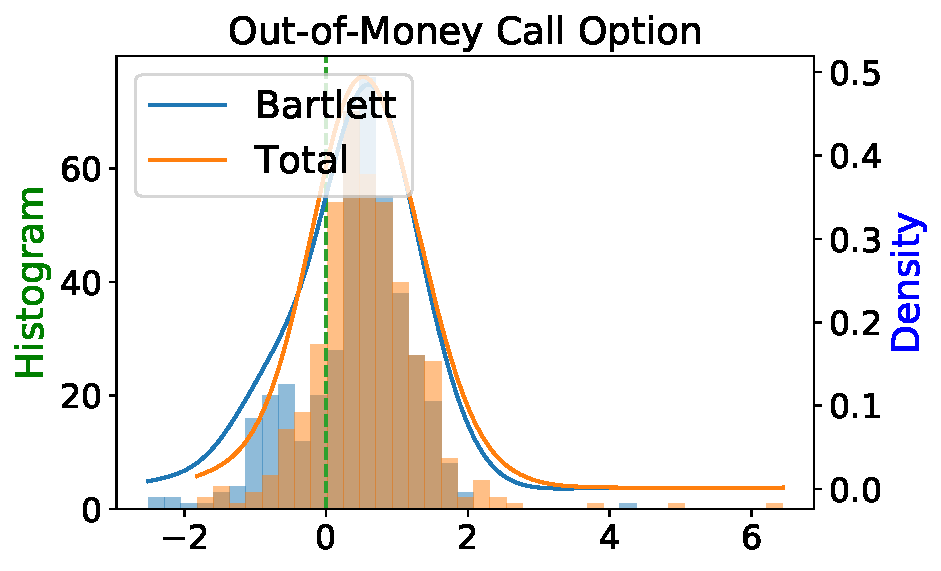
\includegraphics[width=0.32\textwidth]{./figures/WBartlettVersusTotalCallOTM.pdf}}
	\caption{Comparing total model $\modelT$ and Bartlett model on weekly hedging S\&P 500 call options in terms of the distribution of the  relative hedging portfolio value at the expiries.  Please note that the distribution in this figure assumes we are at the sell-side of the option trading.} \label{fig:CallTotalW3}
\end{figure}

From Table \ref{table:CallTotalW}, we can see that, $\modelT$ performs better than the other three methods in terms of 
mean absolute relative hedging error for NTM and OTM scenarios. Although BS model performs slightly better than   $\modelT$ for ITM scenarios. The difference between  $\modelT$  and BS model is small for ITM scenarios. Additionally, $\modelT$, in most of cases, are the besting performing model in terms of VaR and CVaR, indicating that $\modelT$ performs better in reducing tail risk on the loss.  The exceptions are as the following:
\begin{itemize}
	\item $\modelL$ performs best in terms of  CVaR(99\%) for NTM scenarios and ITM scenarios. From Figure \ref{fig:CallTotalW1} (a) and (b), we can see that, the extreme tail on the loss side from  $\modelT$ is worse than than $\modelL$
	\item  BS model performs best in terms of  VaR(99\%) and  CVaR(99\%) for OTM scenarios. This is an interesting observation. From \ref{fig:CallTotalW2} (c), We also note that the extreme tail on the profit side from BS model on OTM scenarios is actually longer than the other three models, indicating a larger probability of getting big profit. 
\end{itemize}

Another interesting observation is that Bartlett delta actually performs worse than BS delta in most of the cases as shown in Table \ref{table:CallTotalW}. We suspect that this is due to the fact that SABR model was originally designed for modeling interest rate derivatives, the time to maturity for which is usually bigger than one-year, and it is less suitable to model option surface with extreme short time to maturity\cite{chen2011calibration}. For weekly hedging, we have used SABR model to produce Bartlett delta with extremely small time to maturity, e.g., 5/250 for the last rebalancing time.
Notice that in chapter \ref{sec:LocalComparison} when we compare models on local risk criteria, options with time-to-expiry less than 14 days are removed from the data set. Therefore, we did not notice this phenomenon.

\subsubsection{Call Option Monthly Hedging Comparison}
In Table \ref{table:CallTotalM}, we demonstrate the results on monthly hedging call options. Furthermore, in Figure \ref{fig:CallTotalM1}, Figure \ref{fig:CallTotalM2}, and  Figure \ref{fig:CallTotalM3}, we compare the distribution of the relative hedging error of $\modelT$ with the distributions of the relative hedging error of $\modelL$, BS model, and Bartlett model respectively.

From Table \ref{table:CallTotalM}, we can see that, $\modelT$ performs better than the other three methods in terms of 
mean absolute relative hedging error for NTM and ITM scenarios. Bartlett method performs best in terms of 
mean absolute relative hedging error for OTM scenarios. In terms of VaR and CVaR, by comparing Table \ref{table:CallTotalM} and Table \ref{table:CallTotalW}, $\modelT$ is less dominant  in monthly hedging call options than in weekly hedging call options. $\modelL$ produces the smallest VaR(95\%) for NTM, ITM and OTM scenarios. Bartlett delta produces best VaR(99\%) and CVaR(99\%) for NTM scenarios. However, from Table \ref{table:CallTotalM} we can also see, the performance of $\modelT$ is usually very close to best performance even if  $\modelT$ is not the dominant model in terms of certain criteria.


On the other hand, from Figure \ref{fig:CallTotalM1} (c) and \ref{fig:CallTotalM2} (c), we can see that, for OTM scenarios, $\modelL$ and BS model produce longer tail on the profit side and  shorter tail on the loss side when comparing with $\modelT$. Besides, from \ref{fig:CallTotalM3} (c), we can see that, for OTM scenarios, Bartlett method has the shorter tail for both the loss side and profit side when comparing with $\modelT$. 
\begin{table}[htp!]
	\centering
	\begin{tabular}{ll|l|l|l|}
		\cline{3-5}
		&          & Near-The-Money   & In-The-Money     & Out-of-The-Money \\ \hline
		\multicolumn{1}{|l|}{\multirow{4}{*}{Mean Abs Error}} & $\modelT$    & \textbf{0.2643}  & \textbf{0.0633}  & 1.0479           \\  
		\multicolumn{1}{|l|}{}                                & $\modelL$    & 0.2740           & 0.0642           & 1.2255           \\  
		\multicolumn{1}{|l|}{}                                & Bartlett & 0.282            & 0.073            & \textbf{0.9674}  \\  
		\multicolumn{1}{|l|}{}                                & BS       & 0.2865           & 0.0655           & 1.3248           \\ \hline
		\multicolumn{1}{|l|}{\multirow{4}{*}{VaR (95\%)}}     & $\modelT$    & -0.4102          & -0.1472          & -1.0842          \\  
		\multicolumn{1}{|l|}{}                                & $\modelL$    & \textbf{-0.3998} & \textbf{-0.1394} & \textbf{-0.9531} \\  
		\multicolumn{1}{|l|}{}                                & Bartlett & -0.4775          & -0.1611          & -1.1936          \\  
		\multicolumn{1}{|l|}{}                                & BS       & -0.5115          & -0.1554          & -1.3442          \\ \hline
		\multicolumn{1}{|l|}{\multirow{4}{*}{CVaR (95\%)}}    & $\modelT$    & \textbf{-0.6073} & \textbf{-0.3125} & \textbf{-1.6658} \\  
		\multicolumn{1}{|l|}{}                                & $\modelL$    & -0.6671          & -0.3144          & -1.6962          \\  
		\multicolumn{1}{|l|}{}                                & Bartlett & -0.6680          & -0.3372          & -2.0221          \\  
		\multicolumn{1}{|l|}{}                                & BS       & -0.9735          & -0.4380          & -2.0016          \\ \hline
		\multicolumn{1}{|l|}{\multirow{4}{*}{VaR (99\%)}}     & $\modelT$    & -0.7752          & \textbf{-0.4300} & \textbf{-1.7567} \\  
		\multicolumn{1}{|l|}{}                                & $\modelL$    & -0.8703          & -0.4329          & -1.9142          \\  
		\multicolumn{1}{|l|}{}                                & Bartlett & \textbf{-0.7201} & -0.4815          & -2.3799          \\  
		\multicolumn{1}{|l|}{}                                & BS       & -1.2384          & -0.6058          & -2.8419          \\ \hline
		\multicolumn{1}{|l|}{\multirow{4}{*}{CVaR (99\%)}}    & $\modelT$    & -0.8692          & \textbf{-0.4627} & -2.7536          \\  
		\multicolumn{1}{|l|}{}                                & $\modelL$    & -1.0861          & -0.4670          & \textbf{-2.5194} \\  
		\multicolumn{1}{|l|}{}                                & Bartlett & \textbf{-0.8090}  & -0.5725          & -2.8797          \\  
		\multicolumn{1}{|l|}{}                                & BS       & -1.2864          & -0.7859          & -3.0839          \\ \hline
	\end{tabular}
	\caption{Summary of monthly hedging S\&P 500 call options for 100 business days with total hedging evaluation criteria. Please note that the total hedging evaluation in this table assumes we are at the sell-side of the option trading.} \label{table:CallTotalM}
\end{table}
\begin{figure}[htp!]
	\centering
	\subfigure[]{
		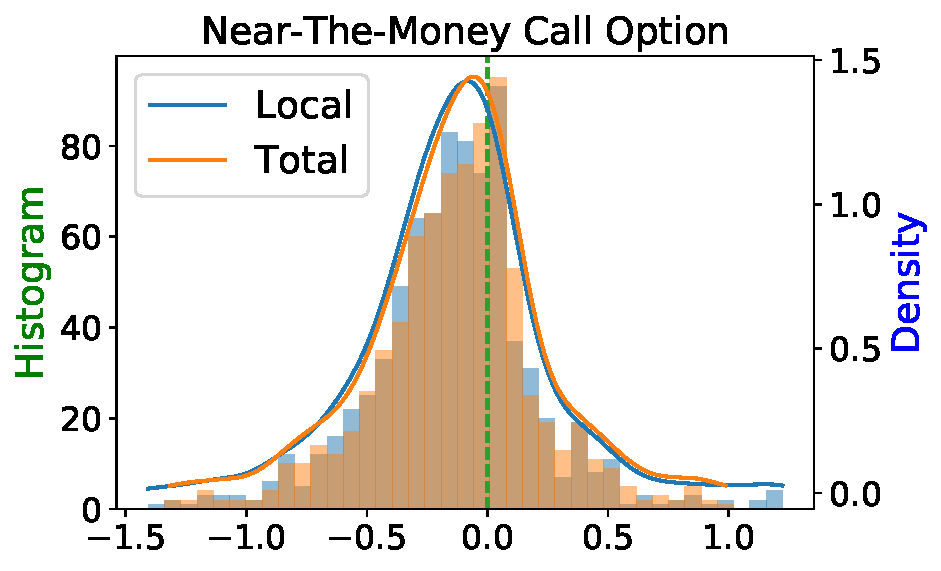
\includegraphics[width=0.32\textwidth]{./figures/MLocalVersusTotalCallNTM.pdf}}
	\subfigure[]{
		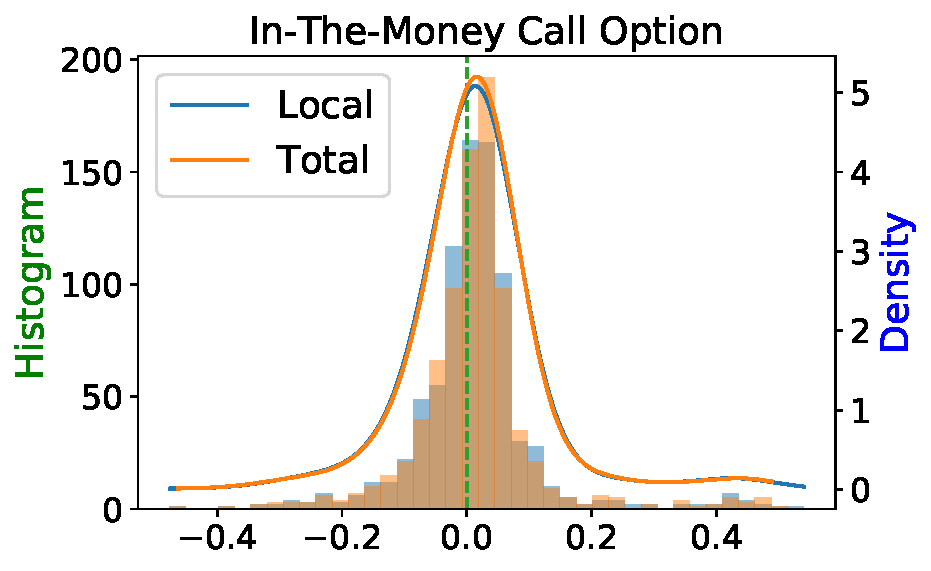
\includegraphics[width=0.32\textwidth]{./figures/MLocalVersusTotalCallITM.pdf}}
	\subfigure[]{
		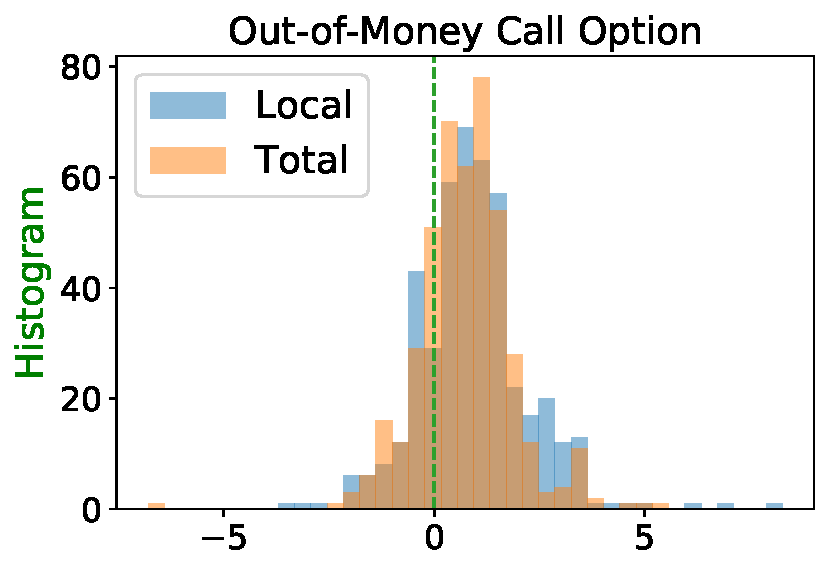
\includegraphics[width=0.32\textwidth]{./figures/MLocalVersusTotalCallOTM.pdf}}
	\caption{Comparing total model $\modelT$ and local model $\modelL$ on monthly hedging S\&P 500 call options in terms of thethe distribution of the  relative hedging portfolio value at the expiries. Please note that the distribution in this figure assumes we are at the sell-side of the option trading.} \label{fig:CallTotalM1}
		\centering
	\subfigure[]{
		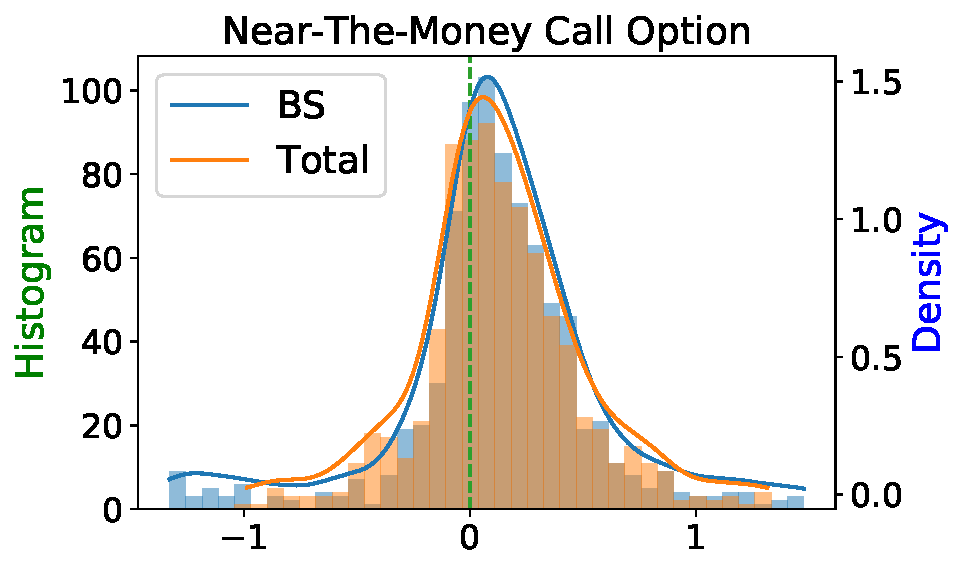
\includegraphics[width=0.32\textwidth]{./figures/MBSVersusTotalCallNTM.pdf}}
	\subfigure[]{
		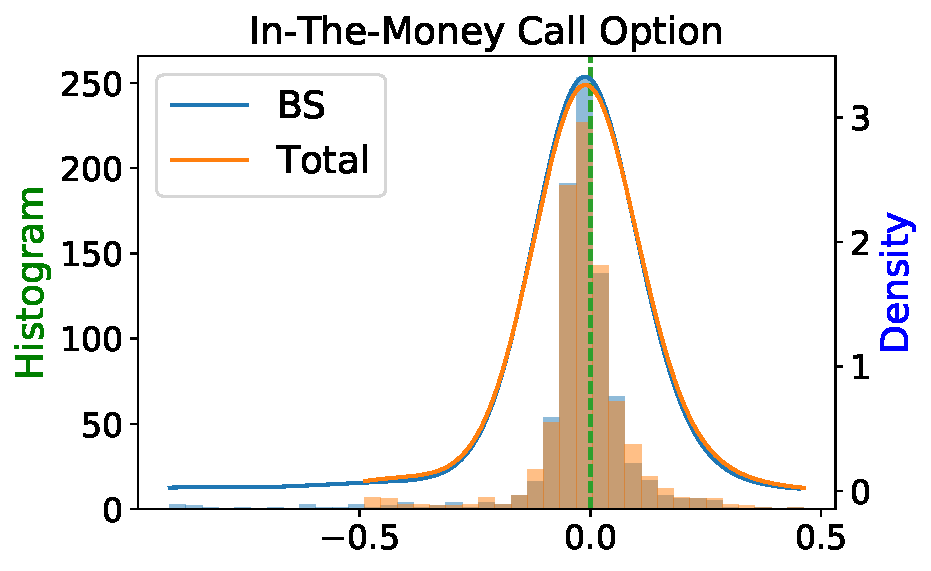
\includegraphics[width=0.32\textwidth]{./figures/MBSVersusTotalCallITM.pdf}}
	\subfigure[]{
		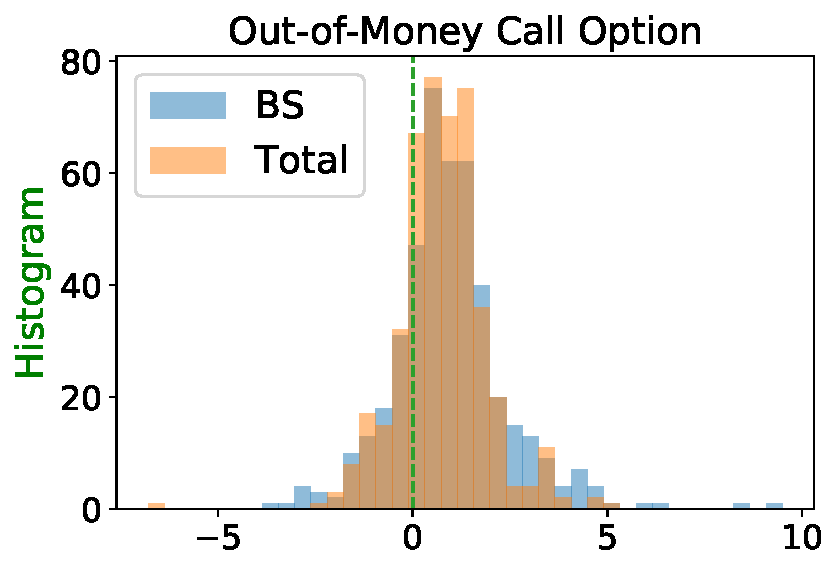
\includegraphics[width=0.32\textwidth]{./figures/MBSVersusTotalCallOTM.pdf}}
	\caption{Comparing total model $\modelT$ and BS model  on monthly hedging S\&P 500 call options in terms of the distribution of the  relative hedging portfolio value at the expiries. Please note that the distribution in this figure assumes we are at the sell-side of the option trading.} 
	\label{fig:CallTotalM2}
		\centering
	\subfigure[]{
		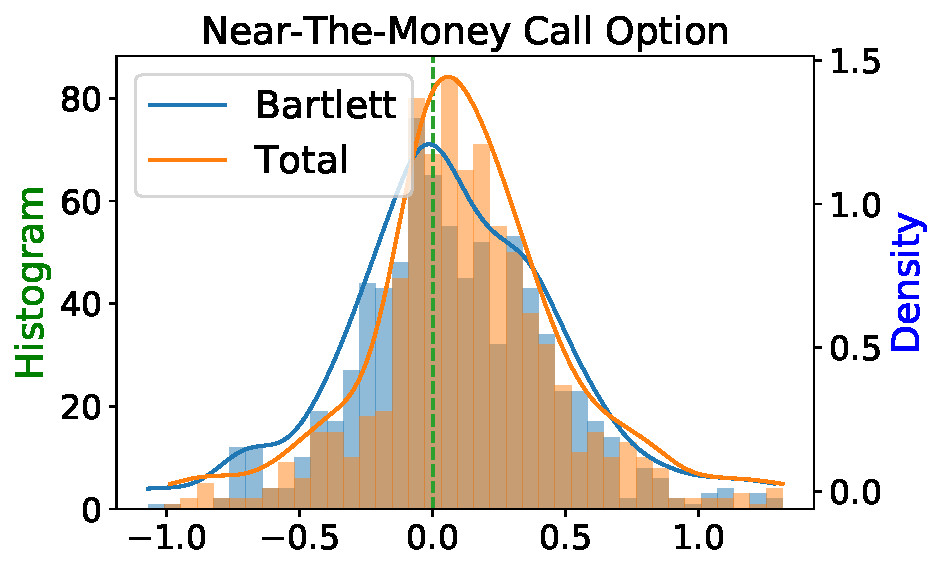
\includegraphics[width=0.32\textwidth]{./figures/MBartlettVersusTotalCallNTM.pdf}}
	\subfigure[]{
		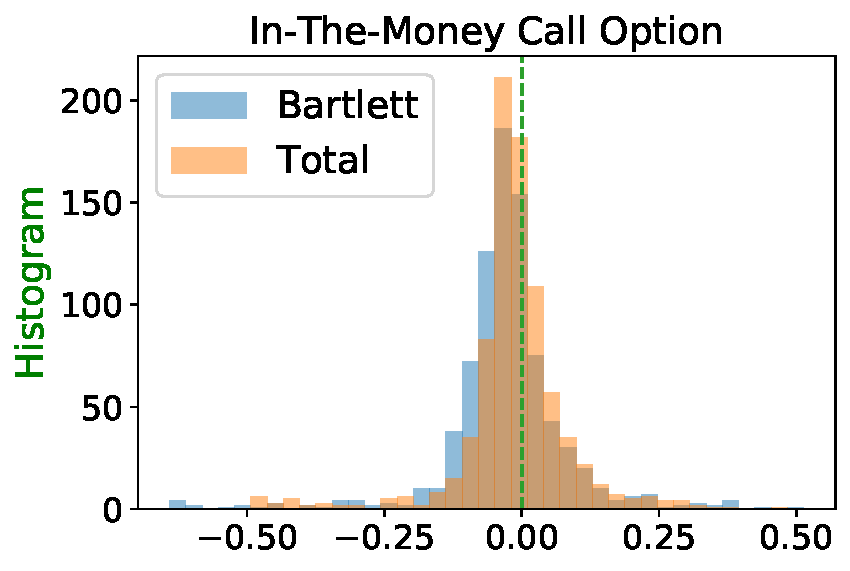
\includegraphics[width=0.32\textwidth]{./figures/MBartlettVersusTotalCallITM.pdf}}
	\subfigure[]{
		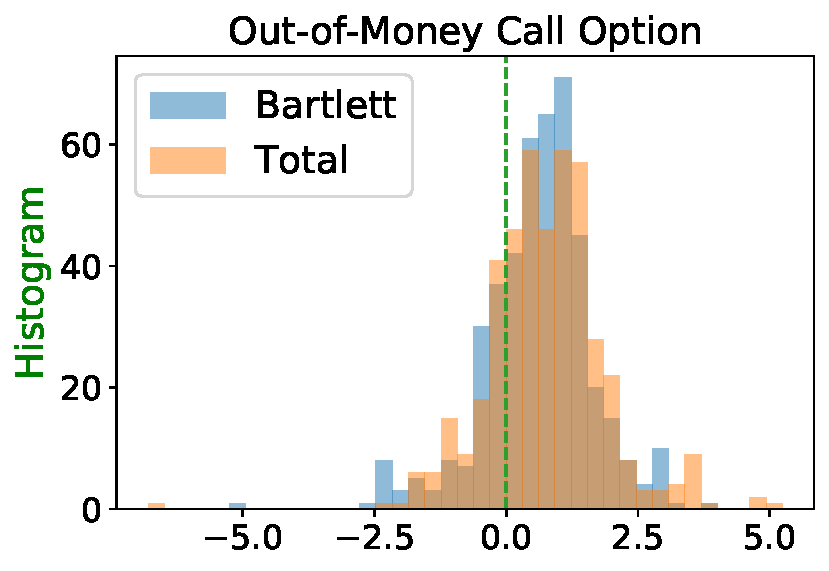
\includegraphics[width=0.32\textwidth]{./figures/MBartlettVersusTotalCallOTM.pdf}}
	\caption{Comparing total model $\modelT$ and bartlett model on monthly hedging S\&P 500 call options in terms of the distribution of the  relative hedging portfolio value at the expiries. Please note that the distribution in this figure assumes we are at the sell-side of the option trading.} \label{fig:CallTotalM3}
\end{figure}

\newpage
\subsection{Put Option Total Hedging Comparison}

In this subsection, we present the results for put options. We again show the hedging performance for Near-The-Money(NTM), In-The-Money(ITM), Out-of-The-Money(OTM) separately.  The NTM, OTM, and ITM scanerios are classified based on the Black-Scholes delta at the initial date $t_0$ where we set up the hedging portfolio: $\delta^{BS}_{t_0,T,K}$. For put option, the criteria is:
\begin{itemize}
	\item  Near-The-Money(NTM): $-0.3 \geq \delta^{BS}_{t_0,T,K} >-0.7$
	\item  In-The-Money(ITM): $-0.7 \geq \delta^{BS}_{t_0,T,K} >-0.95$
	\item  Out-of-The-Money(OTM): $-0.05 \geq \delta^{BS}_{t_0,T,K} >-0.3$
\end{itemize}
We omit the testing scenarios for deep in-the-money and deep out-of-the money options due to the fact that they are highly illiquid in market and their market quotes are highly unreliable. Also, the deep in-the-money and deep out-of-the money options are deleted from training set and validation set.
\begin{itemize}
	\item  Deep Out-of-The-Money(OTM): $0.0 \geq \delta^{BS}_{t_0,T,K} >-0.05$
	\item  Deep In-The-Money(ITM): $-0.95 \geq \delta^{BS}_{t_0,T,K} >-1.0$
\end{itemize}
\subsubsection{Put Option Weekly Hedging Comparison}
In Table \ref{table:putTotalW}, we demonstrate the results on monthly hedging put options. Furthermore, in Figure \ref{fig:putTotalW1}, Figure \ref{fig:putTotalW2}, and  Figure \ref{fig:putTotalW3}, we compare the distribution of the relative hedging error of $\modelT$ with the distributions of the relative hedging error of $\modelL$, BS model, and Bartlett model respectively.

From Table \ref{table:putTotalW}, we can see that, $\modelT$ is the dominant  methods for weekly hedging put options in terms of most of the criteria for NTM, ITM, and OTM scenarios.  There are only two  exception: $\modelL$ performs slightly better than $\modelT$ for NTM scenarios for mean absolute relative hedging error  and Bartlett delta performs performs slightly better than $\modelT$ for OTM scenarios for mean absolute relative hedging error. 

Another interesting observation is that, for put option, the loss tail of the relative hedging distribution is significantly longer than call option. We suspect this is due to the fact that selling put option during market crisis period can lead to significant loss as the original NTM or ITM option can become out-of-the money in a short period of time especially when we are getting closer to the expiry.
\begin{table}[htp!]
	\centering
	\begin{tabular}{ll|l|l|l|}
		\cline{3-5}
		&          & Near-The-Money   & In-The-Money     & Out-of-The-Money  \\ \hline
		\multicolumn{1}{|l|}{\multirow{4}{*}{Mean Abs Error}} & $\modelT$    & 0.2535           & \textbf{0.0965}  & 1.5356   \\ 
		\multicolumn{1}{|l|}{}                                & $\modelL$    & \textbf{0.2516}  & 0.1140           & 1.6042             \\ 
		\multicolumn{1}{|l|}{}                                & Bartlett     & 0.2993 			& 0.167  		   & \textbf{1.4815}       \\ 
		\multicolumn{1}{|l|}{}                                & BS       	 & 0.2773 		    & 0.1227 		   & 1.7109            \\ 
		\hline
		\multicolumn{1}{|l|}{\multirow{4}{*}{VaR (95\%)}}     & $\modelT$    & \textbf{-0.8124} & \textbf{-0.2364} & \textbf{-7.2478}  \\ 
		\multicolumn{1}{|l|}{}                                & $\modelL$    & -0.8229          & -0.3160          & -8.0506           \\ 
		\multicolumn{1}{|l|}{}                                & Bartlett 	 & -0.9374 			& -0.5133 		   &-8.5614           \\  
		\multicolumn{1}{|l|}{}                                & BS       	 & -0.8854 			& -0.4274 		   &-8.7374           \\ 
		\hline
		\multicolumn{1}{|l|}{\multirow{4}{*}{CVaR (95\%)}}    & $\modelT$    & \textbf{-1.0475} & \textbf{-0.3452} & \textbf{-10.9438} \\ 
		\multicolumn{1}{|l|}{}                                & $\modelL$    & -1.2335          & -0.5405          & -11.8778          \\  
		\multicolumn{1}{|l|}{}                                & Bartlett 	 & -1.4781  		&-0.8078 		   &-12.2226          \\  
		\multicolumn{1}{|l|}{}                                & BS       	 &  -1.4812  		&-0.7236 		   &-13.3299          \\ 
		\hline
		\multicolumn{1}{|l|}{\multirow{4}{*}{VaR (99\%)}}     & $\modelT$    & \textbf{-1.1138} & \textbf{-0.3763} & \textbf{-11.7573} \\  
		\multicolumn{1}{|l|}{}                                & $\modelL$    & -1.4361          & -0.7996          & -14.5369           \\ 
		\multicolumn{1}{|l|}{}                                & Bartlett 	 & -1.6118  		 &-0.99   		   &-12.2933         \\  
		\multicolumn{1}{|l|}{}                                & BS       	 & -1.7625  		&-0.7979 		   &-19.0822          \\ 
		\hline
		\multicolumn{1}{|l|}{\multirow{4}{*}{CVaR(99\%)}}     & $\modelT$    & \textbf{-1.3597} & \textbf{-0.4616} & \textbf{-15.1555} \\  
		\multicolumn{1}{|l|}{}                                & $\modelL$    & -1.7732          & -0.9739          & -17.0642         \\ 
		\multicolumn{1}{|l|}{}                                & Bartlett     &-2.3355  			&-1.2264 		   &-17.4385          \\ 
		\multicolumn{1}{|l|}{}                                & BS       	 & -2.2831  		&-1.1347 		   &-20.6413          \\ \hline
	\end{tabular}
	\caption{Summary of weekly hedging S\&P 500 put options for 100 Business days with total hedging evaluation criteria. Please note that the total hedging evaluation in this table assumes we are at the sell-side of the option trading.} \label{table:putTotalW}
\end{table}
\begin{figure}[htp!]
	\centering
	
	\subfigure[]{
		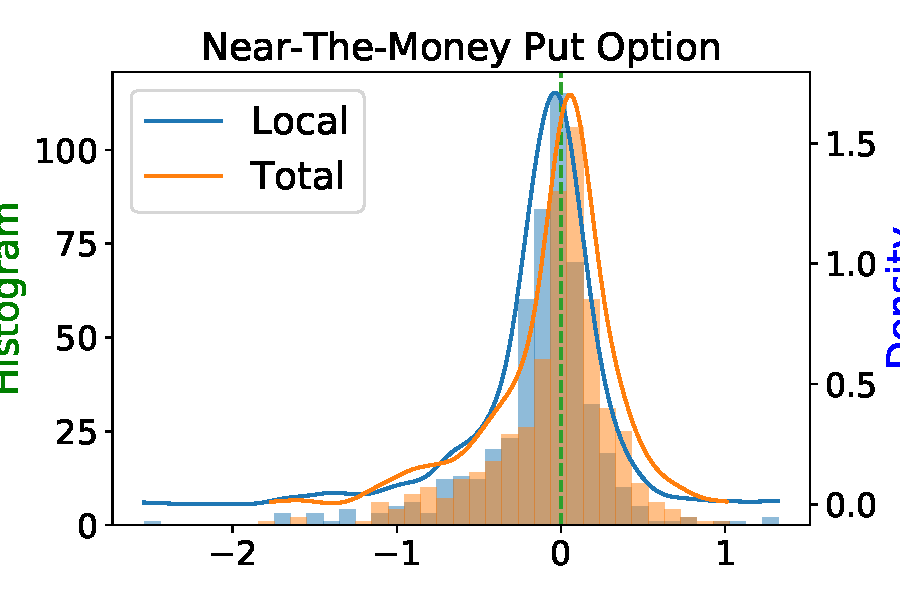
\includegraphics[width=0.32\textwidth]{./figures/LocalVersusTotalNTM.pdf}}
	\subfigure[]{
		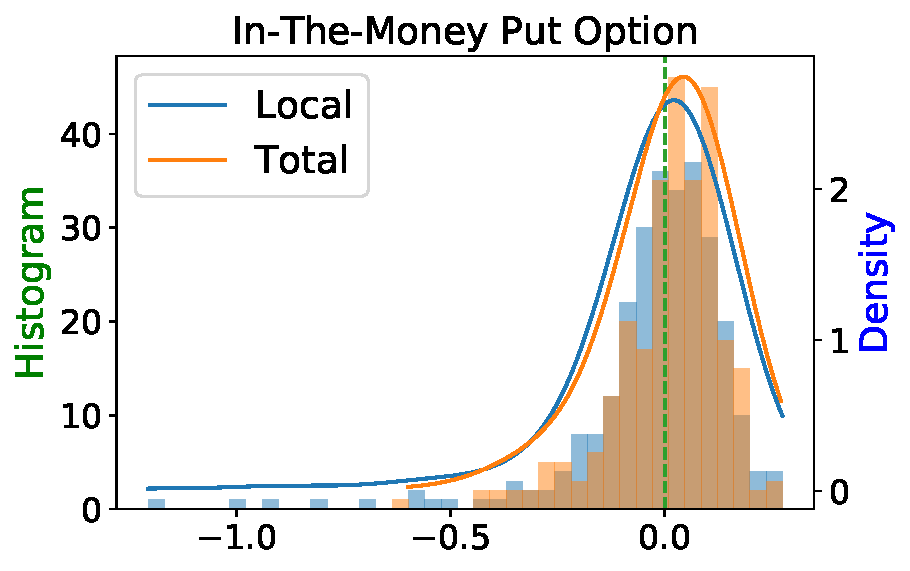
\includegraphics[width=0.32\textwidth]{./figures/LocalVersusTotalITM.pdf}}
	\subfigure[]{
		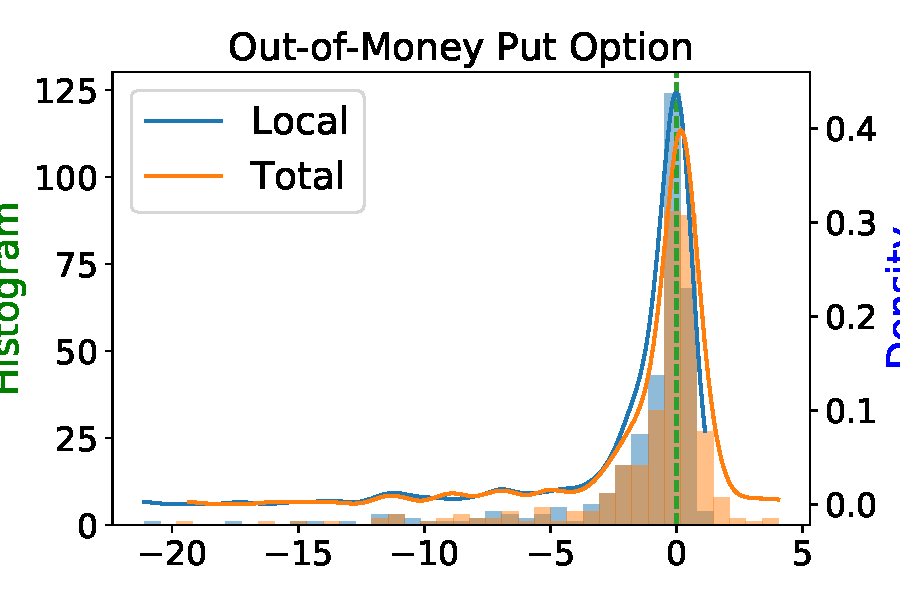
\includegraphics[width=0.32\textwidth]{./figures/LocalVersusTotalOTM.pdf}}
	\caption{Comparing total model $\modelT$ and local model $\modelL$ on weekly hedging put options in terms of the distribution of the  relative hedging portfolio value at the expiries. Please note that the distribution in this figure assumes we are at the sell-side of the option trading.} \label{fig:putTotalW1}
	\centering
	\subfigure[]{
		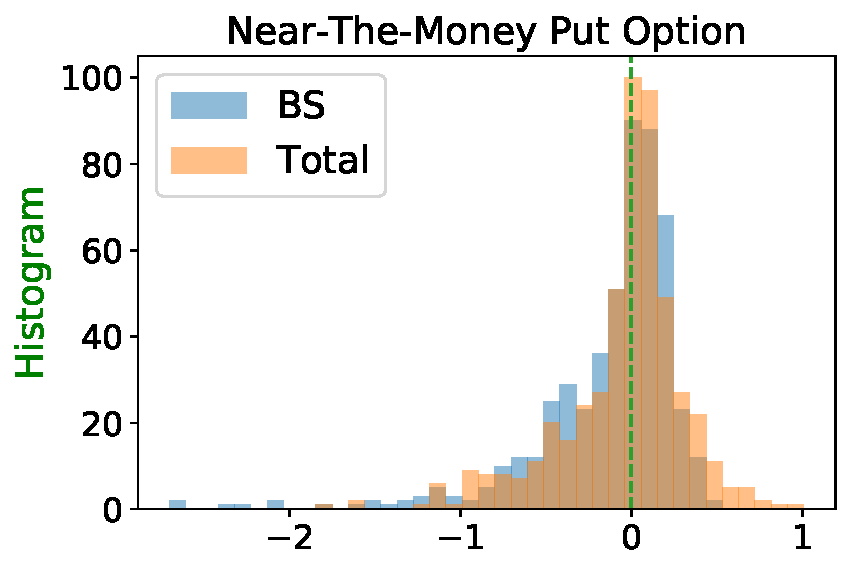
\includegraphics[width=0.32\textwidth]{./figures/BSVersusTotalNTM.pdf}}
	\subfigure[]{
		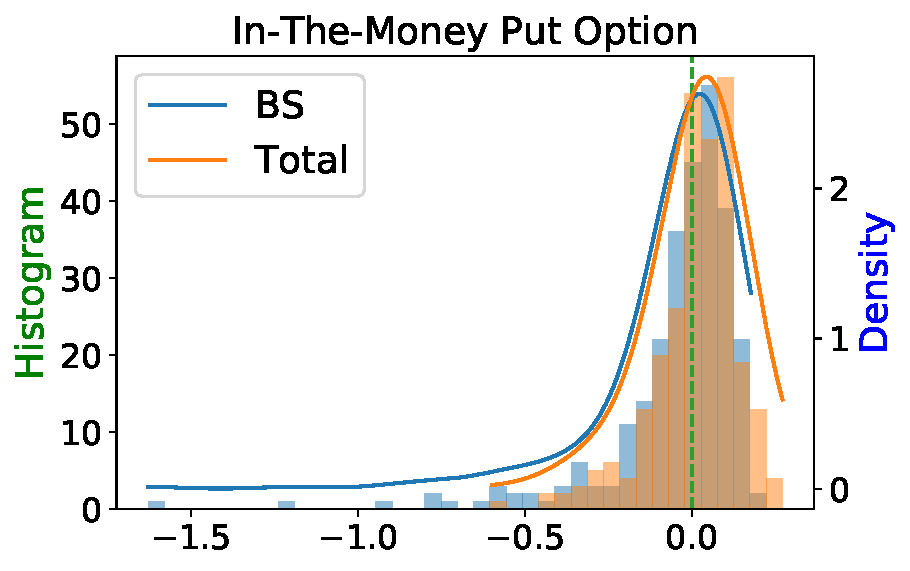
\includegraphics[width=0.32\textwidth]{./figures/BSVersusTotalITM.pdf}}
	\subfigure[]{
		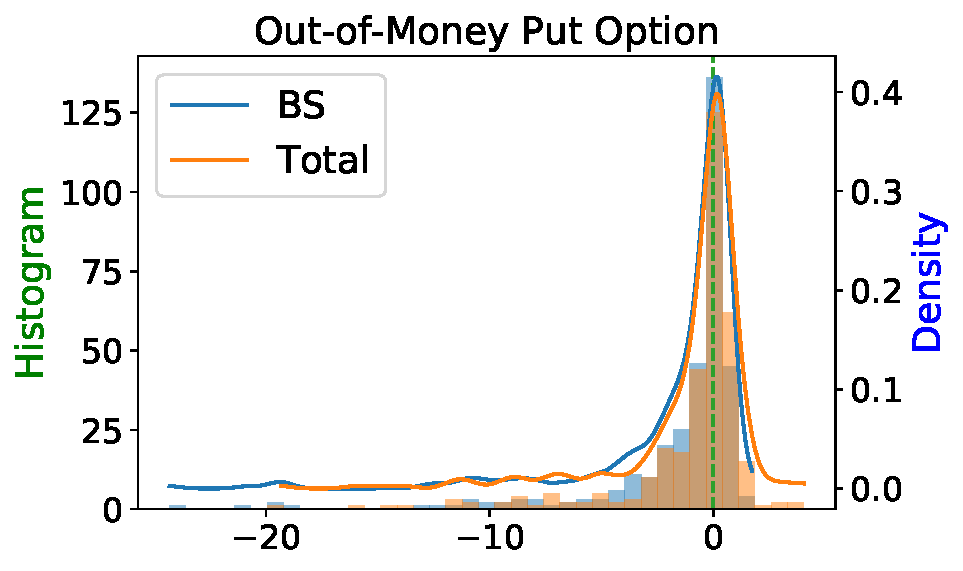
\includegraphics[width=0.32\textwidth]{./figures/BSVersusTotalOTM.pdf}}
	\caption{Comparing total model $\modelT$ and BS model on weekly hedging put options in terms of the distribution of the  relative hedging portfolio value at the expiries. Please note that the distribution in this figure assumes we are at the sell-side of the option trading.} \label{fig:putTotalW3}
		\centering
	\subfigure[]{
		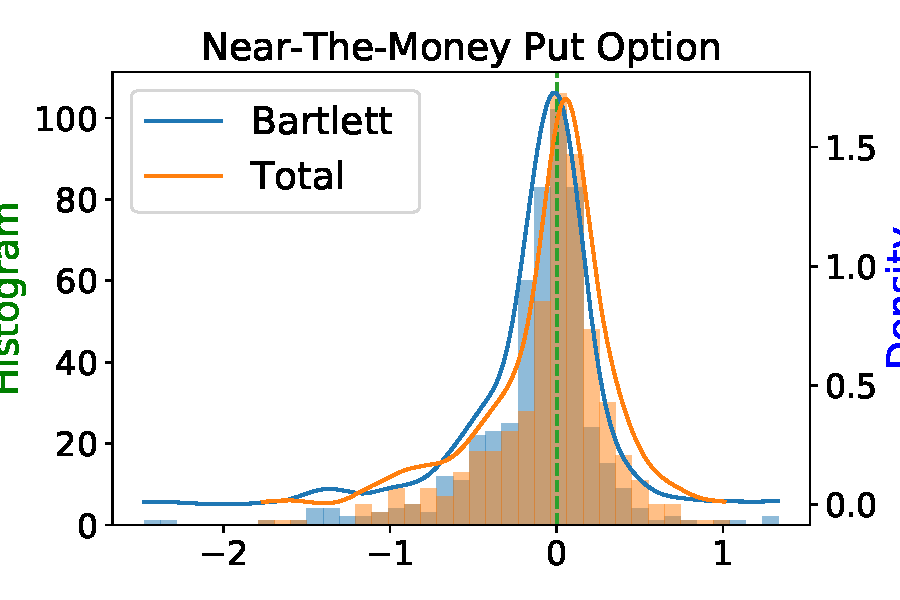
\includegraphics[width=0.32\textwidth]{./figures/BartlettVersusTotalNTM.pdf}}
	\subfigure[]{
		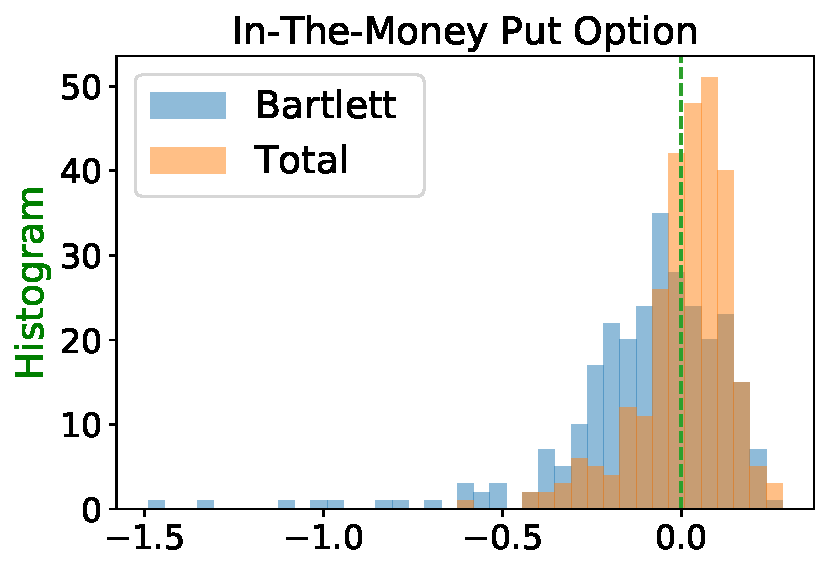
\includegraphics[width=0.32\textwidth]{./figures/BartlettVersusTotalITM.pdf}}
	\subfigure[]{
		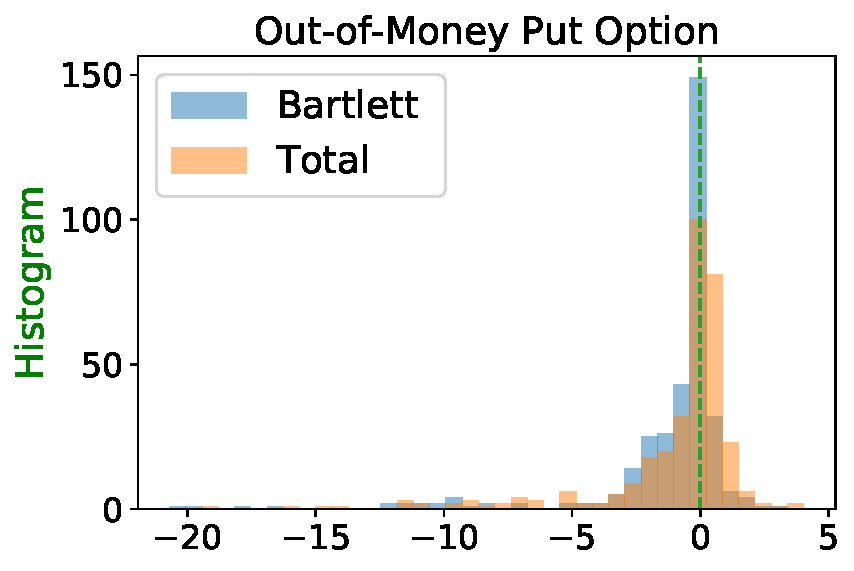
\includegraphics[width=0.32\textwidth]{./figures/BartlettVersusTotalOTM.pdf}}
	\caption{Comparing total model $\modelT$ and Bartlett model on weekly hedging put options in terms of the distribution of the  relative hedging portfolio value at the expiries. Please note that the distribution in this figure assumes we are at the sell-side of the option trading.} \label{fig:putTotalW2}
\end{figure}

\newpage
\subsubsection{Put Option Monthly Hedging Comparison}
In Table \ref{table:putTotalM}, we demonstrate the results on monthly hedging put options. Furthermore, in Figure \ref{fig:putTotalM1}, Figure \ref{fig:putTotalM2}, and  Figure \ref{fig:putTotalM3}, we compare the distribution of the relative hedging error of $\modelT$ with the distributions of the relative hedging error of $\modelL$, BS model, and Bartlett model respectively.

From Table \ref{table:putTotalM}, we can see that, $\modelT$ is still the dominant  method for monthly hedging put options in terms of most of the criteria for NTM, ITM, and OTM scenarios.  However, by comparing Table \ref{table:putTotalW} and Table \ref{table:putTotalM}, we can see $\modelT$ is less dominant in monthly hedging than in weekly hedging. In certain case, Bartlett methods can perform much better. For instance, for NTM scenarios, the CVaR (95\%) and CVaR (99\%) from Bartlett method is significantly better than the other three comparing methods.
\begin{table}[htp!]
	\centering
	\begin{tabular}{ll|l|l|l|}
		\cline{3-5}
		&          & Near-The-Money   & In-The-Money     & Out-of-The-Money  \\ \hline
		\multicolumn{1}{|l|}{\multirow{4}{*}{Mean Abs Error}} & $\modelT$    & \textbf{0.2986}  & \textbf{0.1240}  & 1.7639            \\  
		\multicolumn{1}{|l|}{}                                & $\modelL$    & 0.3485           & 0.1394           & \textbf{1.6849}   \\  
		\multicolumn{1}{|l|}{}                                & Bartlett & 0.3205           & 0.1583           & 1.7383            \\  
		\multicolumn{1}{|l|}{}                                & BS       & 0.3224           & 0.1342           & 1.8482            \\ \hline
		\multicolumn{1}{|l|}{\multirow{4}{*}{VaR (95\%)}}     & $\modelT$    & \textbf{-0.7395} & \textbf{-0.2562} & -8.5602           \\  
		\multicolumn{1}{|l|}{}                                & $\modelL$    & -0.7558          & -0.3268          & \textbf{-8.1812}  \\  
		\multicolumn{1}{|l|}{}                                & Bartlett & -0.8370          & -0.3583          & -9.0303           \\  
		\multicolumn{1}{|l|}{}                                & BS       & -0.7768          & -0.3088          & -9.7018           \\ \hline
		\multicolumn{1}{|l|}{\multirow{4}{*}{CVaR (95\%)}}    & $\modelT$    & -1.7761          & \textbf{-0.3577} & \textbf{-13.3160} \\  
		\multicolumn{1}{|l|}{}                                & $\modelL$    & -1.8144          & -0.4898          & -14.6857          \\  
		\multicolumn{1}{|l|}{}                                & Bartlett & \textbf{-1.5710} & -0.6016          & -14.4425          \\  
		\multicolumn{1}{|l|}{}                                & BS       & -1.8682          & -0.5401          & -16.1024          \\ \hline
		\multicolumn{1}{|l|}{\multirow{4}{*}{VaR (99\%)}}     & $\modelT$    & -2.1792          & \textbf{-0.4121} & -15.2323          \\  
		\multicolumn{1}{|l|}{}                                & $\modelL$    & \textbf{-2.1577} & -0.6454          & -16.5192          \\  
		\multicolumn{1}{|l|}{}                                & Bartlett & -2.9164          & -0.7728          & \textbf{-15.0144} \\  
		\multicolumn{1}{|l|}{}                                & BS       & -2.5569          & -0.7583          & -15.8393          \\ \hline
		\multicolumn{1}{|l|}{\multirow{4}{*}{CVaR (99\%)}}    & $\modelT$    & -3.4001          & \textbf{-0.4509}  & \textbf{-20.6503} \\  
		\multicolumn{1}{|l|}{}                                & $\modelL$    & -3.3717          & -0.6910          & -21.7928          \\  
		\multicolumn{1}{|l|}{}                                & Bartlett & \textbf{-2.9164} & -0.8463          & -24.1757          \\  
		\multicolumn{1}{|l|}{}                                & BS       & -3.5486          & -0.8109          & -26.4941          \\ \hline
	\end{tabular}
	\caption{Summary of monthly hedging S\&P 500 put options for 100 business days with total hedging evaluation criteria. Please note that the total hedging evaluation in this table assumes we are at the sell-side of the option trading.}
	\label{table:putTotalM}
\end{table}
\begin{figure}[htp!]
	\centering
	\subfigure[]{
		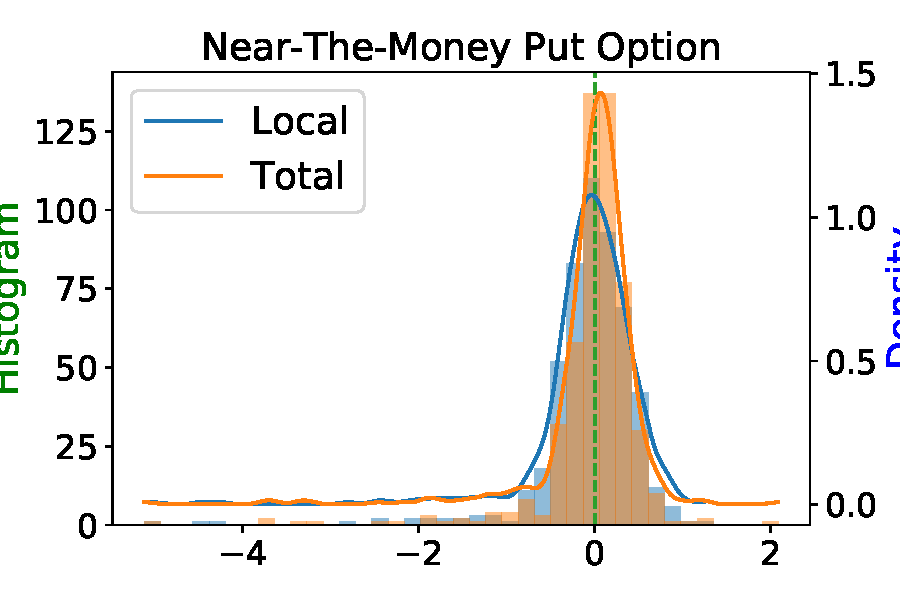
\includegraphics[width=0.32\textwidth]{./figures/MLocalVersusTotalNTM.pdf}}
	\subfigure[]{
		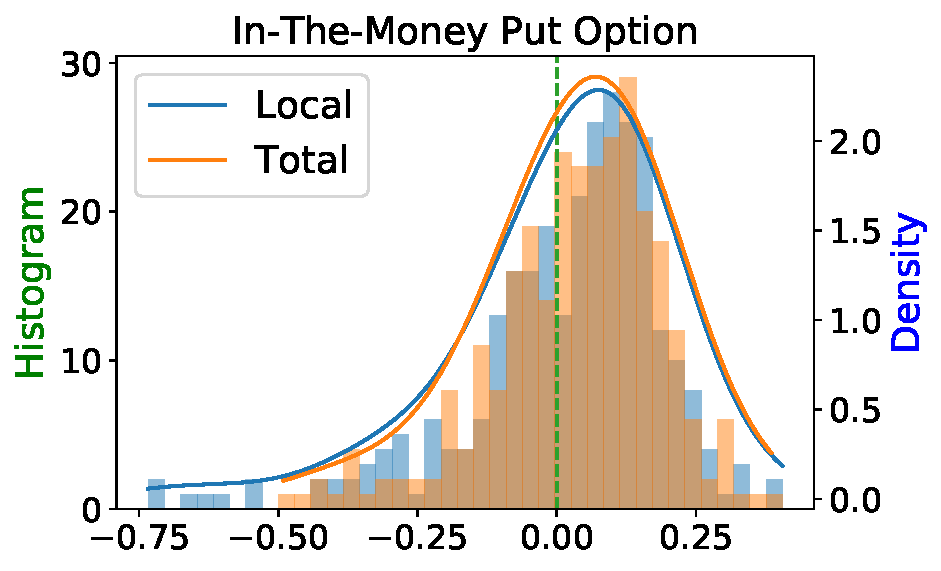
\includegraphics[width=0.32\textwidth]{./figures/MLocalVersusTotalITM.pdf}}
	\subfigure[]{
		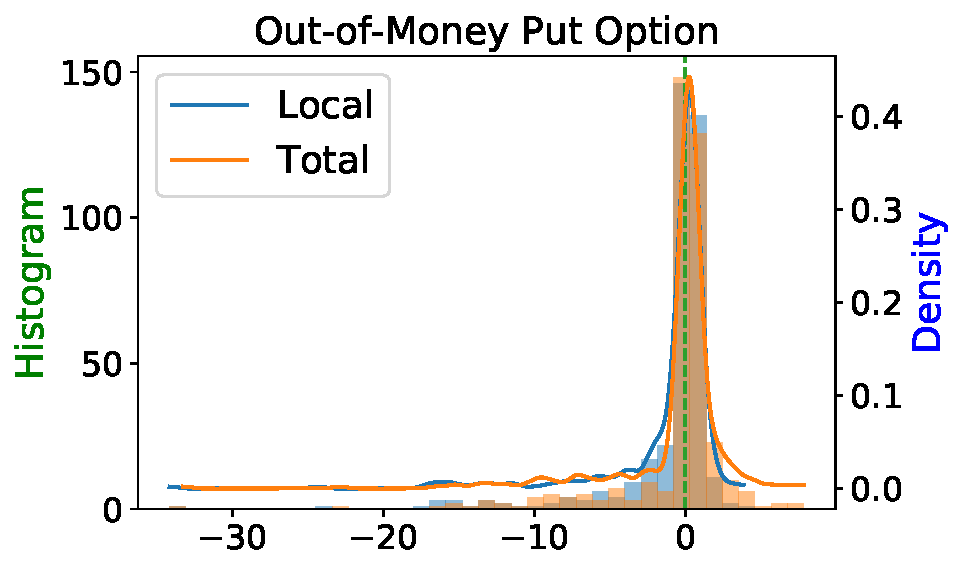
\includegraphics[width=0.32\textwidth]{./figures/MLocalVersusTotalOTM.pdf}}
	\caption{Comparing total model $\modelT$ and local model $\modelL$ on monthly hedging put options in terms of the distribution of the  relative hedging portfolio value at the expiries. Please note that the distribution in this figure assumes we are at the sell-side of the option trading.} \label{fig:putTotalM1}
	\centering
	\subfigure[]{
	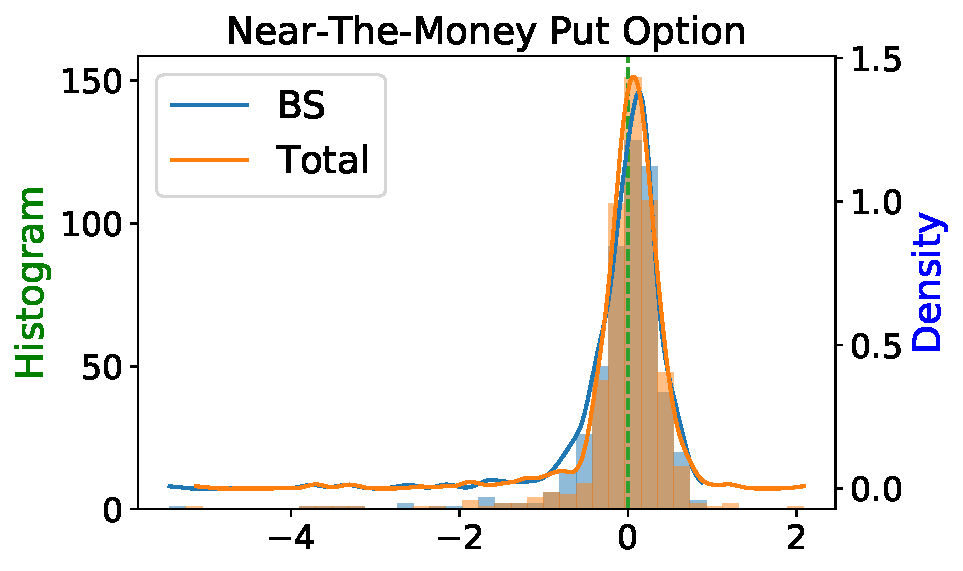
\includegraphics[width=0.32\textwidth]{./figures/MBSVersusTotalNTM.pdf}}
\subfigure[]{
	\includegraphics[width=0.32\textwidth]{./figures/MBSVersusTotalITM.pdf}}
\subfigure[]{
	\includegraphics[width=0.32\textwidth]{./figures/MBSVersusTotalOTM.pdf}}
		\caption{Comparing total model $\modelT$ and BS model on monthly hedging put options in terms of the distribution of the  relative hedging portfolio value at the expiries. Please note that the distribution in this figure assumes we are at the sell-side of the option trading.}  \label{fig:putTotalM2}
	\centering
		\subfigure[]{
		\includegraphics[width=0.32\textwidth]{./figures/MBartlettVersusTotalNTM.pdf}}
	\subfigure[]{
		\includegraphics[width=0.32\textwidth]{./figures/MBartlettVersusTotalITM.pdf}}
	\subfigure[]{
		\includegraphics[width=0.32\textwidth]{./figures/BartlettVersusTotalOTM.pdf}}
		\caption{Comparing total model $\modelT$ and Bartlett model on monthly hedging put options in terms of the distribution of the  relative hedging portfolio value at the expiries. Please note that the distribution in this figure assumes we are at the sell-side of the option trading.} \label{fig:putTotalM3}
\end{figure}
Another interesting observation is that the $\modelT$ produces longer tail for NTM and OTM scenarios on the profit side while for ITM scenarios, $\modelT$  has a much shorter tail on the loss side.
\chapter{Conclusion and Future Work}
\label{sec:Conclusion}

In this thesis, we have proposed a direct kernel hedging model $\DKLs$ and a novel encoder-decoder  model, $\model$ , for discrete local risk option hedging. The $\DKLs$ is our preliminary exploration on computing a data-driven local hedging model without estimating a option pricing model. The $\model$ is our enhancement to data-driven local hedging model. $\model$ consists of an encoder, which generates a concise representation of the past market  information. The decoder uses the Black-Scholes delta as a pre-trained model and utilizes a gate to generate a predicative hedging model,  combining the pre-trained delta model and the outputs from the encoder. Feature selections are implemented through normalized weights embedded in the model training. In addition, a data instance adaptive Huber loss function is incorporated  for robustness, with the error from the pre-trained Black-Scholes delta model for each instance as the thresholding parameter. 

Using the S\&P 500 index and the index option data,  from January 1, 2004, to  August 31st, 2015, we assess and compare hedging performance of the  $\model$ and $\DKLs$ with other hedging strategies in terms of local risk criteria.
For weekly and monthly hedging, computational results demonstrate that performance of the proposed $\model$  significantly surpasses that of the MV model , SABR-Bartlett, regularized spline kernel model $\DKLs$ , all of which perform significantly better than the Black–Scholes model with implied volatility.
In addition, the $\DKLs$ also outperforms MV model in terms of weekly and monthly hedging results.
We further demonstrate that the encoder for the sequential features plays a significant role in $\model$, since removing the encoder deteriorates hedging performance.
Lastly, by comparing the weekly and monthly hedging performance from $\textsc{GRU}_{c}$ and $\model$, we demonstrate that the output gate,  robust loss and training procedure, also play  significant roles in $\model$.

We further demonstrate that the daily hedging performance of the proposed $\model$  also surpasses that of the MV hedging method , LVF and SABR corrective methods  (implemented in \cite{hulloptimal}), data-driven regularized spline kernel network model $\DKLs$ , and SABR-Bartlett. In addition, $\DKLs$ also outperforms MV hedging method , LVF and SABR corrective methods  (implemented in \cite{hulloptimal}).

Besides, from the testing hedging performance, we assess feature importance in  $\model$  for the S\&P 500 index  option hedging. The monthly average feature weights identify the underlying as the most important local feature and the past implied volatility sequence as the most important sequential feature during normal market periods.

To cope with total hedging scenarios, we derive a total risk model $\modelT$ from $\model$ to extend the data-driven model to multi-step total hedging scenarios.  To cope with the challenges of acquiring enough market option information for building data-driven hedging models,  we augment the market data using SABR model and local volatility model. Using the S\&P 500 index  option market data from January 2, 2000 to  August 31st, 2015, we compare  the weekly and monthly hedging performance of the proposed total hedging model $\modelT$  with the sequential data-driven local hedging model $\modelL$, which adopts the same model structure but is trained with a local risk training objective, and the SABR-Bartlett method \cite{bartlett2006hedging}. We measure the total hedging performance, which is evaluated on the expiries of the option. We demonstrate the effectiveness of the total hedging model $\modelT$ in reducing the sell-side loss tail risk for both put and call options. We also demonstrate that the  total hedging model $\modelT$ often leads to better hedging performance in terms of total hedging criteria when compared with $\modelL$,  SABR-Bartlett method, and Black-Scholes model.  Lastly, we demonstrate that the $\modelT$ still performs reasonably well when we switch to buy-side except for monthly hedging OTM put option at buy-side, where $\modelT$ performs the worst in terms of VaR and CVaR.  We  provide some potential explanations for the poor performance of $\modelT$ on monthly hedging OTM put option at buy-side and leave it as the future work of extending our study.


The main objective of this research  is to assess hedging performance of strategies learned  directly from the  historical time series of the market option price and underlying price,  using machine learning methods. Hedging  performance comparisons between data-driven  models $\DKLs$, $\model$, $\modelT$,and  $\modelL$ and the  classical  option hedging based on parametric model calibration suggest that the data driven  learning hedging can be a viable alternative to the classical methods,  potentially leading to better hedging performance.  

In terms of limitation of this research, we compare the data-driven models majorly with parametric models available in academic literature.  We understand that the actual industry practice may not apply the parametric models in the same way as we did in this thesis for hedging derivatives.
While it would also  be interesting to compare hedging methods actually adopted in the financial industry,   limitation in accessing actual industry practice makes it difficult to conduct such a study and make its results publicly available.

Additionally, comparing with the calibration of the traditional parametric pricing models, the learning process for the data-driven hedging model is less computationally efficient. Lastly, the learning process requires certain amount of historical data. For calibrating a parametric model, one usually needs much less data and  can  build the model based on market data observed on spot and compute the sensitivity as hedging position accordingly.  Therefore, our proposed data-driven models are not directly applicable to the illiquid derivative markets.  



For extending our work, we note that there are several directions:
\begin{itemize}
	\item In this thesis, we rely on market data to gather the hedging scenarios.  The volatility surface is calibrated from market data and underlying price paths are extracted from market with overlapping period. Our models based on neural network approach contains less parameters compared with other applications of the deep learning techniques given the relative scarcity of available historical data. 
	For future work, one can explore how we can use machine learning techniques to generate hedging scenarios so that we can combine artificial scenarios with real scenarios. This will enable us to build more complex model for hedging.
	Indeed, for this direction, there are already several attempts. For example, \citet{bergeron2021variational} apply the variational autoencoders \cite{kingma2013auto} on generating synthetic volatility surface  that are indistinguishable from those observed historically. \citet{pardo2020mitigating} apply the  Generative Adversarial Networks (GANs) \cite{goodfellow2014generative} on learning  the underlying structure inherent to the dynamics of financial series and acquiring the capacity to generate scenarios that share many similarities to those seen in the historic  time series.  
	\item In this thesis, we use S\&P 500 index options for experimental comparison. It is interesting to explore on the effectiveness of the data-driven models on more complex derivatives such as basket options where the dimensionality of the underlying is higher. 
	\item In this thesis, we have not include transaction cost into our models. A more realistic model should include the effect of the transaction cost as in \cite{buehler2019deep}. 
	\item  In this thesis, for total hedging  model, we assume we rebalance every 5 business days or 20 business days. In reality, we do not have to fix the time gap between two rebalancing time. We can extend the model so that the data-driven model determines when is the best time to rebalance the hedging portfolio. 
\end{itemize}


%----------------------------------------------------------------------
% END MATERIAL
%----------------------------------------------------------------------

% B I B L I O G R A P H Y
% -----------------------

% The following statement selects the style to use for references.  It controls the sort order of the entries in the bibliography and also the formatting for the in-text labels.
\bibliographystyle{plainnat}
% This specifies the location of the file containing the bibliographic information.
% It assumes you're using BibTeX (if not, why not?).
\cleardoublepage % This is needed if the book class is used, to place the anchor in the correct page,
                 % because the bibliography will start on its own page.
                 % Use \clearpage instead if the document class uses the "oneside" argument
\phantomsection  % With hyperref package, enables hyperlinking from the table of contents to bibliography
% The following statement causes the title "References" to be used for the bibliography section:
\renewcommand*{\bibname}{References}

% Add the References to the Table of Contents
\addcontentsline{toc}{chapter}{\textbf{References}}

\bibliography{uw-ethesis}
% Tip 5: You can create multiple .bib files to organize your references.
% Just list them all in the \bibliogaphy command, separated by commas (no spaces).

% The following statement causes the specified references to be added to the bibliography% even if they were not
% cited in the text. The asterisk is a wildcard that causes all entries in the bibliographic database to be included (optional).
\nocite{*}

% The \appendix statement indicates the beginning of the appendices.
%\appendix
%\addcontentsline{toc}{chapter}{APPENDICES}
% Add a title page before the appendices and a line in the Table of Contents
%\chapter{Total Hedging Comparison on Synthetic Scenarios}
%\label{sec:SynCompara}
%\section{Black-Scholes Model}
%We adopt the same experimental setting as \cite{coleman2007total}. Specifically, we assume $S_0=100$,$K=100$, $T=1$, $\mu=0.15$,$r=0.04$, and $\sigma=0.2$.
%We have 600 time steps with $\Delta t=1/600$. We can hedge every 25,50,100,300 time steps.
%\begin{table}[htp!]
%\centering
%\begin{tabular}{|c|c|c|c|c|}
%  \hline
%  % after \\: \hline or \cline{col1-col2} \cline{col3-col4} ...
%  method       &25 &50&100&300 \\
%  GRU          & 0.8448& 1.1845& 1.6518 & 2.7989 \\
%  GRU (Refined)& 0.8376& 1.1426& 1.6896 & 2.8038 \\
%  Spline       & 0.8563& 1.1789& 1.6518 & 2.7843 \\
%  Analytical   & 0.8295& 1.1636& 1.6479 & 2.7914 \\
%  Delta        & 0.9481&1.3385 & 1.9128 & 3.4582 \\
%  \hline
%\end{tabular}
%\caption{Total Risk}
%\end{table}
%
%
%\begin{table}[htp!]
%\centering
%\begin{tabular}{|c|c|c|c|c|}
%  \hline
%  % after \\: \hline or \cline{col1-col2} \cline{col3-col4} ...
%  method &25 &50&100&300 \\
%  GRU          & 5.8943& 5.8812& 5.7378 & 5.2507 \\
%  GRU (Refined)& 5.9682& 5.8370& 5.8549 & 5.1759 \\
%  Spline    & 5.9118& 5.8445& 5.7119 & 5.2530 \\
%  Analytical& 5.9413& 5.8773& 5.7399 & 5.2565 \\
%  Delta     & 6.0483& 6.0897& 6.1734 & 6.5382 \\
%  \hline
%\end{tabular}
%\caption{Total Cost}
%\end{table}
\newpage
\appendix

\chapter{Sell-Side Risk Versus Buy-Side Risk}
In previous section, we mainly evaluate the hedging performance assuming we are at the sell-side of the option trading. Namely, we assume that we are shorting an option. In this subsection, we look at the risk on the buy-side.  More specifically, assuming we are now at the buy-side of the option trading, we set up the hedging portfolio as:
\begin{itemize}
	\item A long position on option $\Vmkt(t,T,K)$
	\item Short $-\delta^{M}_{t,T,K}$ (or long if $\delta^{M}_{t,T,K}<0$ ) shares of $\Smkt(t)$
	\item An amount in a risk-free bank account $B(t)$
\end{itemize}

Let $P^{B}_H(T,T,H)$ be the hedging portfolio value of the buy-side at the expiry. One can easily verify that:
$P^{B}_H(T,T,H)=-P_H(T,T,H)$, where $P_H(T,T,H)$ is the side-side  hedging portfolio value at the expiry given by equation \eqref{eq:FinalHValue}. The profit  on the sell-side  hedging portfolio ( $P_H(T,T,H)>0$) becomes the loss on the  buy-side hedging portfolio ( $P^B_H(T,T,H)<0$). In other words, if we notice that we have a long tail on the profit side of PnL (Profit and Loss) distribution at the sell-side, then we will have a long tail on the loss side of PnL distribution at the buy-side. We notice from the analysis of distribution of relative hedging error in previous section, with $\modelT$ and $\modelL$, the sell-side loss is reduced significantly. But we also noticed that this reduction of the sell-side loss sometimes comes with a increase of the loss on the buy-side. Meanwhile, we also notice this kind of trade-off also exists for BS model and Bartlett model.

To complete our comparison, we evaluate the total hedging performance using the following 4 criteria for the buy-side hedging portfolio $P^{B}_H(T,T,H)$:
\begin{enumerate}

	\item The 95\% Value-at-Risk (VaR) of the relative total hedging error $\frac{D(t_0,T) P^B_H(T,T,K)}{\Vmkt_{t_0,T,K}}$
	\item The 95\% Conditional-Value-at-Risk (CVaR) of the relative total hedging error $\frac{D(t_0,T) P^B_H(T,T,K)}{\Vmkt_{t_0,T,K}}$
	\item The 99\% Value-at-Risk (VaR) of the relative total hedging error $\frac{D(t_0,T) P^B_H(T,T,K)}{\Vmkt_{t_0,T,K}}$
	\item The 99\% Conditional-Value-at-Risk (CVaR) of the relative total hedging error $\frac{D(t_0,T) P^B_H(T,T,K)}{\Vmkt_{t_0,T,K}}$
\end{enumerate}
Please note that $P^B_H(T,T,K)=-P_H(T,T,H)$.

\subsubsection{Comparing Sell-Side Risk with Buy-Side Risk on Call Option}
In Table \ref{table:CallTotalWBuy} and  Table \ref{table:CallTotalMBuy},  we demonstrate the results on weekly and monthly hedging call options at buy-side.
\begin{table}[htp!]
	\centering
	\begin{tabular}{ll|l|l|l|}
		\cline{3-5}
		&          & Near-The-Money   & In-The-Money     & Out-of-The-Money \\ \hline
		\multicolumn{1}{|l|}{\multirow{4}{*}{Mean Abs Error}} & $\modelT$     & \textbf{0.1927}  & 0.0571           		 & \textbf{0.7344}   \\  
		\multicolumn{1}{|l|}{}                                & $\modelL$     & 0.2250           & 0.0866          		 	 & 0.8285            \\  
		\multicolumn{1}{|l|}{}                                & Bartlett      & 0.2347           & 0.0641           		 & 0.7383            \\  
		\multicolumn{1}{|l|}{}                                & BS            & 0.2198           & \textbf{0.0531}  		 & 0.9706            \\ 
		\hline
		\multicolumn{1}{|l|}{\multirow{4}{*}{VaR (95\%)}}     & $\modelT$     & -0.5189          & -0.1054 					 & -1.6139  \\  
		\multicolumn{1}{|l|}{}                                & $\modelL$     & -0.5692          & -0.1763          		 & -1.9182           \\  
		\multicolumn{1}{|l|}{}                                & Bartlett      & \textbf{-0.4630} & -0.0880          		 & \textbf{-1.5149}           \\  
		\multicolumn{1}{|l|}{}                                & BS            & -0.4931          & \textbf{-0.0696}          & -2.6341           \\ 
		\hline
		\multicolumn{1}{|l|}{\multirow{4}{*}{CVaR (95\%)}}    & $\modelT$     & -0.6464 		 & -0.1509 					 & -2.3918  \\  
		\multicolumn{1}{|l|}{}                                & $\modelL$     & -0.7062          & -0.2377          		 & -2.4369          \\  
		\multicolumn{1}{|l|}{}                                & Bartlett      & \textbf{-0.5731} & -0.1632          		 & \textbf{-1.7694}          \\  
		\multicolumn{1}{|l|}{}                                & BS            & -0.6833          & \textbf{-0.1157}          & -3.8273           \\ 
		\hline
		\multicolumn{1}{|l|}{\multirow{4}{*}{VaR (99\%)}}     & $\modelT$     & -0.7778 		 & -0.1861 					 & -2.5132           \\  
		\multicolumn{1}{|l|}{}                                & $\modelL$     & -0.8034          & -0.2769          		 & -2.3604           \\  
		\multicolumn{1}{|l|}{}                                & Bartlett      & \textbf{-0.6284} & -0.2477          		 & \textbf{-1.7751}           \\  
		\multicolumn{1}{|l|}{}                                & BS            & -0.7510          & \textbf{-0.1524}          & -3.2443 			\\ 
		\hline
		\multicolumn{1}{|l|}{\multirow{4}{*}{CVaR (99\%)}}    & $\modelT$     & -0.8180          & -0.2093                   & -3.8272           \\  
		\multicolumn{1}{|l|}{}                                & $\modelL$     & -0.8837 		 & -0.2965  		         & -3.5071          \\  
		\multicolumn{1}{|l|}{}                                & Bartlett      & \textbf{-0.7426} & -0.2617          		 & \textbf{-2.2728}           \\  
		\multicolumn{1}{|l|}{}                                & BS            & -0.8699          & \textbf{-0.1173}          & -5.9191 			\\ 
		\hline
	\end{tabular}
	\caption{Summary of weekly hedging S\&P 500 call options for 100 business days with total hedging evaluation criteria. Please note that the total hedging evaluation in this table assumes we are at the buy-side of the option trading.} \label{table:CallTotalWBuy}
\end{table}
\begin{table}[htp!]
	\centering
	\begin{tabular}{ll|l|l|l|}
		\cline{3-5}
		&          & Near-The-Money   & In-The-Money     & Out-of-The-Money \\ \hline
		\multicolumn{1}{|l|}{\multirow{4}{*}{Mean Abs Error}} & $\modelT$    & \textbf{0.2643}  & \textbf{0.0633}  & 1.0479           \\  
		\multicolumn{1}{|l|}{}                                & $\modelL$    & 0.2740           & 0.0642           & 1.2255           \\  
		\multicolumn{1}{|l|}{}                                & Bartlett 	 & 0.282            & 0.073            & \textbf{0.9674}  \\  
		\multicolumn{1}{|l|}{}                                & BS       	 & 0.2865           & 0.0655           & 1.3248           \\ 
		\hline
		\multicolumn{1}{|l|}{\multirow{4}{*}{VaR (95\%)}}     & $\modelT$    & -0.7194  		& -0.1313 		   			&-2.4261       \\  
		\multicolumn{1}{|l|}{}                                & $\modelL$    & -0.6955			& -0.1365 		   			&-3.1978 \\  
		\multicolumn{1}{|l|}{}                                & Bartlett 	 &\textbf{-0.6504} 	&-0.1238 		   			&\textbf{-2.1608}          \\  
		\multicolumn{1}{|l|}{}                                & BS       	 & -0.7312 			&\textbf{-0.1128} 		   & -3.5289        \\ 
		\hline 
		\multicolumn{1}{|l|}{\multirow{4}{*}{CVaR (95\%)}}    & $\modelT$    &-0.9148 			&-0.2181 		   		  &-3.4331 \\  
		\multicolumn{1}{|l|}{}                                & $\modelL$    &-0.9315 			&-0.2191 		   		   &-3.9418         \\  
		\multicolumn{1}{|l|}{}                                & Bartlett 	 &\textbf{-0.8779}  &-0.2345           		   &\textbf{-2.7161}          \\  
		\multicolumn{1}{|l|}{}                                & BS       	 &-1.0158 			&\textbf{-0.1907} 		   &-4.711          \\ 
		\hline
		\multicolumn{1}{|l|}{\multirow{4}{*}{VaR (99\%)}}     & $\modelT$    & -1.0753 			& -0.2751 		   			&-3.5691       \\  
		\multicolumn{1}{|l|}{}                                & $\modelL$    &-1.0929 			&-0.2768 		   			&-4.062         \\  
		\multicolumn{1}{|l|}{}                                & Bartlett 	 &\textbf{-1.0468}  &-0.3147           			&\textbf{-2.9381}         \\  
		\multicolumn{1}{|l|}{}                                & BS       	 &-1.2136 			& \textbf{-0.2348} 		    & -4.8304         \\ 
		\hline
		\multicolumn{1}{|l|}{\multirow{4}{*}{CVaR (99\%)}}    & $\modelT$    &-1.1926 			&-0.3272 		    & -4.2966          \\  
		\multicolumn{1}{|l|}{}                                & $\modelL$    &-1.2134 			&-0.3283 		    & -5.7881         \\  
		\multicolumn{1}{|l|}{}                                & Bartlett 	 &\textbf{-1.1678}  &-0.3810            &\textbf{-3.1807}          \\  
		\multicolumn{1}{|l|}{}                                & BS       	 &-1.3321 			&\textbf{-0.2948}   & -6.651          \\ 
		\hline
	\end{tabular}
	\caption{Summary of monthly hedging S\&P 500 call options for 100 business days with total hedging evaluation criteria. Please note that the total hedging evaluation in this table assumes we are at the buy-side of the option trading.} \label{table:CallTotalMBuy}
\end{table}
By comparing Table \ref{table:CallTotalW} and Table \ref{table:CallTotalWBuy} and  comparing table \ref{table:CallTotalW} and Table \ref{table:CallTotalWBuy}, we have the  following observations:
\begin{enumerate}
	\item In terms of VaR and CVaR, Bartlett delta is the worst model on the sell-side for weekly  hedging NTM and OTM call options as shown in Table \ref{table:CallTotalW}. But when we  switch to buy-side, for weekly hedging NTM and OTM call options, Bartlett delta is the best performing  model in terms of VaR and CVaR as shown in Table \ref{table:CallTotalWBuy}.
	
	\item  When we  switch to buy-side, for monthly hedging NTM and OTM call options, Bartlett delta is the best performing  model in terms of VaR and CVaR as shown in Table \ref{table:CallTotalMBuy}. At the sell-side as shown in  Table \ref{table:CallTotalM}, for OTM Call options, Bartlett delta is the second worst performing model in terms of VaR and CVaR.
	
	\item In terms of VaR and CVaR, BS delta is the worst model on the sell-side for weekly  and monthly hedging ITM call option as shown in Table \ref{table:CallTotalW} and Table \ref{table:CallTotalM}. But when we switch to buy-side,   BS delta is the best performing  model in terms of VaR and CVaR as shown in table  Table \ref{table:CallTotalWBuy} and Table \ref{table:CallTotalMBuy}. Additionally, for weekly hedging OTM option, the BS delta produces the smallest VaR(99\%) and CVaR(99\%) on the sell-side but the largest VaR(99\%) and CVaR(99\%) on the buy-side.
	\item At the buy-side, for weekly and monthly hedging call option, $\modelT$  is neither the worst performing model nor the best performing model in terms of VaR and CVaR. 
	\item The $\modelT$ usually is the best or the second best model in terms of VaR and CVaR no matter we are at sell-side or buy-side for weekly and monthly hedging call option,  as shown in Table \ref{table:CallTotalW}, Table \ref{table:CallTotalWBuy} , Table \ref{table:CallTotalM} and Table \ref{table:CallTotalMBuy}.
\end{enumerate}
\subsubsection{Comparing Sell-Side Risk with Buy-Side Risk on Put Option}
In Table \ref{table:putTotalWBuy} and  Table \ref{table:putTotalMBuy},  we demonstrate the results on weekly and monthly hedging put options at buy-side. We notice the following by comparing Table \ref{table:putTotalWBuy} and  Table \ref{table:putTotalW} comparing Table \ref{table:putTotalMBuy} and  Table \ref{table:putTotalM}:
\begin{enumerate}
	\item The $\modelT$ usually is the best or the second best model in terms of VaR and CVaR  at sell-side for weekly and monthly hedging put option,  as shown in Table \ref{table:putTotalW} and Table \ref{table:putTotalM}. As one can see the reduction at the loss tail from $\modelT$ at the sell-side is significant when compared with other models. When we switch to buy-side, the data-driven model $\modelT$ still performs reasonably well in terms of VaR and CVaR. $\modelT$ usually is the second best performing model at the buy-side for reducing the weekly hedging loss tail when compared with the BS model.
	
	However, when we switch to buy-side as shown in Table \ref{table:putTotalMBuy},  $\modelT$ does not perform well in terms of VaR and CVaR for monthly hedging OTM options. We suspect this is due to the fact that the distribution of relative hedging error for monthly hedging put options is very unbalanced as one can see in Figure \ref{fig:putTotalM1} to \ref{fig:putTotalM3}. The heavily unbalanced nature of the hedging error distribution potentially damaged the performance of the $\modelT$ at buy-side for monthly hedging OTM options.  We leave resolving this issue as the future work of our study.
	
\item	 In terms of VaR and CVaR, BS delta is the worst model or the second worst on the sell-side for weekly  and monthly hedging  put option as shown in Table \ref{table:putTotalW} and Table \ref{table:putTotalM}. But when we switch to buy-side,   BS delta is the best performing or the second best  model in terms of VaR and CVaR as shown in table  Table \ref{table:putTotalWBuy} and Table \ref{table:putTotalMBuy}. Additionally, for monthly hedging OTM option, the BS delta produces the smallest VaR(99\%) and CVaR(99\%) on the buy-side but the largest VaR(99\%) and CVaR(99\%) on the sell-side.
\item	 At the sell-side,  $\modelL$ significantly reduces the loss tail when compared with BS delta on weekly and monthly hedging put options.
 At the buy-side, the performance from $\modelL$ is very close to BS delta on monthly and weekly hedging OTM put options.  $\modelL$ either underperforms or outperforms BS delta slightly on weekly and monthly hedging put options at the buy-side.


\end{enumerate}

\begin{table}[htp!]
	\centering
	\begin{tabular}{ll|l|l|l|}
		\cline{3-5}
		&          & Near-The-Money   & In-The-Money     & Out-of-The-Money  \\ \hline
		\multicolumn{1}{|l|}{\multirow{4}{*}{Mean Abs Error}} & $\modelT$    & 0.2535           & \textbf{0.0965}  & 1.5356   \\ 
		\multicolumn{1}{|l|}{}                                & $\modelL$    & \textbf{0.2516}  & 0.1140           & 1.6042             \\ 
		\multicolumn{1}{|l|}{}                                & Bartlett     & 0.2993 			& 0.167  		   & \textbf{1.4815}       \\ 
		\multicolumn{1}{|l|}{}                                & BS       	 & 0.2773 		    & 0.1227 		   & 1.7109            \\ 
		\hline
		\multicolumn{1}{|l|}{\multirow{4}{*}{VaR (95\%)}}     & $\modelT$    &-0.4113 &-0.1754 &-1.2127  \\ 
		\multicolumn{1}{|l|}{}                                & $\modelL$    &-0.3063 &-0.1659 &\textbf{-0.5048}           \\ 
		\multicolumn{1}{|l|}{}                                & Bartlett 	 &-0.294  &-0.1614 &-0.6739           \\  
		\multicolumn{1}{|l|}{}                                & BS       	 &\textbf{-0.2692} &\textbf{-0.1398} &-0.6120           \\ 
		\hline
		\multicolumn{1}{|l|}{\multirow{4}{*}{CVaR (95\%)}}    & $\modelT$    &-0.589  &-0.2041 &-1.9494 \\ 
		\multicolumn{1}{|l|}{}                                & $\modelL$    &-0.5611 &-0.2055 &\textbf{-0.8351}         \\  
		\multicolumn{1}{|l|}{}                                & Bartlett 	 &-0.4056 &-0.2046 &-1.2439          \\  
		\multicolumn{1}{|l|}{}                                & BS       	 &\textbf{-0.3515} &\textbf{-0.1594} &-0.8701          \\ 
		\hline
		\multicolumn{1}{|l|}{\multirow{4}{*}{VaR (99\%)}}     & $\modelT$    &-0.6983 &-0.2252 &-2.3629 \\  
		\multicolumn{1}{|l|}{}                                & $\modelL$    &-0.6925 &-0.2389 &-1.052           \\ 
		\multicolumn{1}{|l|}{}                                & Bartlett 	 &-0.4668 &-0.2222 &-1.5293         \\  
		\multicolumn{1}{|l|}{}                                & BS       	 &\textbf{-0.4108} &\textbf{-0.171}  &\textbf{-1.0188}          \\ 
		\hline
		\multicolumn{1}{|l|}{\multirow{4}{*}{CVaR(99\%)}}     & $\modelT$    &-0.7835 &-0.2476 &-3.2214 \\  
		\multicolumn{1}{|l|}{}                                & $\modelL$    &-0.9811 &-0.2498 &\textbf{-1.2042}         \\ 
		\multicolumn{1}{|l|}{}                                & Bartlett     &-0.6232 &-0.2415 &-2.0532          \\ 
		\multicolumn{1}{|l|}{}                                & BS       	 &\textbf{-0.4383} &\textbf{-0.1741} &-1.2597          \\ \hline
	\end{tabular}
	\caption{Summary of weekly hedging S\&P 500 put options for 100 Business days with total hedging evaluation criteria. Please note that the total hedging evaluation in this table assumes we are at the sell-side of the option trading.} \label{table:putTotalWBuy}
\end{table}

\begin{table}[htp!]
	\centering
	\begin{tabular}{ll|l|l|l|}
		\cline{3-5}
		&          & Near-The-Money   & In-The-Money     & Out-of-The-Money  \\ \hline
		\multicolumn{1}{|l|}{\multirow{4}{*}{Mean Abs Error}} & $\modelT$    & \textbf{0.2986}  & \textbf{0.1240}  & 1.7639            \\  
		\multicolumn{1}{|l|}{}                                & $\modelL$    & 0.3485           & 0.1394           & \textbf{1.6849}   \\  
		\multicolumn{1}{|l|}{}                                & Bartlett & 0.3205           & 0.1583           & 1.7383            \\  
		\multicolumn{1}{|l|}{}                                & BS       & 0.3224           & 0.1342           & 1.8482            \\ 
		\hline
		\multicolumn{1}{|l|}{\multirow{4}{*}{VaR (95\%)}}     & $\modelT$    &\textbf{-0.504}  &-0.2428 &-2.519           \\  
		\multicolumn{1}{|l|}{}                                & $\modelL$    &-0.5766 &-0.2363 &-1.2493  \\  
		\multicolumn{1}{|l|}{}                                & Bartlett 	 &-0.4788 &\textbf{-0.1968} &-1.2757           \\  
		\multicolumn{1}{|l|}{}                                & BS       	 &-0.518  &-0.2159 &\textbf{-0.9276}           \\ 
		\hline
		\multicolumn{1}{|l|}{\multirow{4}{*}{CVaR (95\%)}}    & $\modelT$    &-0.7372 &-0.2905 &-4.2365 \\  
		\multicolumn{1}{|l|}{}                                & $\modelL$    &-0.7496 &-0.2924 &-1.8623          \\  
		\multicolumn{1}{|l|}{}                                & Bartlett 	 &-0.6301 &\textbf{-0.2556} &-2.4399          \\  
		\multicolumn{1}{|l|}{}                                & BS       	 &\textbf{-0.6164} &-0.2816 &\textbf{-1.5589}          \\ 
		\hline
		\multicolumn{1}{|l|}{\multirow{4}{*}{VaR (99\%)}}     & $\modelT$   &-0.7195 &-0.3177 &-5.3271         \\  
		\multicolumn{1}{|l|}{}                                & $\modelL$   &-0.8031 &-0.332  &-2.0655
		                  \\  
		\multicolumn{1}{|l|}{}                                & Bartlett 	& -0.7157 &\textbf{-0.2898} &-3.0177\\  
		\multicolumn{1}{|l|}{}                                & BS       	&\textbf{-0.6555} &-0.3227 &\textbf{-1.7745}         \\ 
		\hline
		\multicolumn{1}{|l|}{\multirow{4}{*}{CVaR (99\%)}}    & $\modelT$   &-1.1155 &-0.3448 &-6.6073 \\  
		\multicolumn{1}{|l|}{}                                & $\modelL$   &-0.9367 &-0.3655 &-2.87          \\  
		\multicolumn{1}{|l|}{}                                & Bartlett 	&-0.8404 &\textbf{-0.3353} &-4.1933          \\  
		\multicolumn{1}{|l|}{}                                & BS       	&\textbf{-0.7283} &-0.3498 &\textbf{-2.4294}          \\ 
		\hline
	\end{tabular}
	\caption{Summary of monthly hedging S\&P 500 put options for 100 business days with total hedging evaluation criteria. Please note that the total hedging evaluation in this table assumes we are at the buy-side of the option trading.}
	\label{table:putTotalMBuy}
\end{table}

\end{document}
